\documentclass[twoside]{book}

% Packages required by doxygen
\usepackage{calc}
\usepackage{doxygen}
\usepackage{graphicx}
\usepackage[utf8]{inputenc}
\usepackage{makeidx}
\usepackage{multicol}
\usepackage{multirow}
\usepackage{textcomp}
\usepackage[table]{xcolor}

% Font selection
\usepackage[T1]{fontenc}
\usepackage{mathptmx}
\usepackage[scaled=.90]{helvet}
\usepackage{courier}
\usepackage{amssymb}
\usepackage{sectsty}
\renewcommand{\familydefault}{\sfdefault}
\allsectionsfont{%
  \fontseries{bc}\selectfont%
  \color{darkgray}%
}
\renewcommand{\DoxyLabelFont}{%
  \fontseries{bc}\selectfont%
  \color{darkgray}%
}

% Page & text layout
\usepackage{geometry}
\geometry{%
  a4paper,%
  top=2.5cm,%
  bottom=2.5cm,%
  left=2.5cm,%
  right=2.5cm%
}
\tolerance=750
\hfuzz=15pt
\hbadness=750
\setlength{\emergencystretch}{15pt}
\setlength{\parindent}{0cm}
\setlength{\parskip}{0.2cm}
\makeatletter
\renewcommand{\paragraph}{%
  \@startsection{paragraph}{4}{0ex}{-1.0ex}{1.0ex}{%
    \normalfont\normalsize\bfseries\SS@parafont%
  }%
}
\renewcommand{\subparagraph}{%
  \@startsection{subparagraph}{5}{0ex}{-1.0ex}{1.0ex}{%
    \normalfont\normalsize\bfseries\SS@subparafont%
  }%
}
\makeatother

% Headers & footers
\usepackage{fancyhdr}
\pagestyle{fancyplain}
\fancyhead[LE]{\fancyplain{}{\bfseries\thepage}}
\fancyhead[CE]{\fancyplain{}{}}
\fancyhead[RE]{\fancyplain{}{\bfseries\leftmark}}
\fancyhead[LO]{\fancyplain{}{\bfseries\rightmark}}
\fancyhead[CO]{\fancyplain{}{}}
\fancyhead[RO]{\fancyplain{}{\bfseries\thepage}}
\fancyfoot[LE]{\fancyplain{}{}}
\fancyfoot[CE]{\fancyplain{}{}}
\fancyfoot[RE]{\fancyplain{}{\bfseries\scriptsize Generated on Fri Jul 28 2017 23\-:05\-:12 for librpc by Doxygen }}
\fancyfoot[LO]{\fancyplain{}{\bfseries\scriptsize Generated on Fri Jul 28 2017 23\-:05\-:12 for librpc by Doxygen }}
\fancyfoot[CO]{\fancyplain{}{}}
\fancyfoot[RO]{\fancyplain{}{}}
\renewcommand{\footrulewidth}{0.4pt}
\renewcommand{\chaptermark}[1]{%
  \markboth{#1}{}%
}
\renewcommand{\sectionmark}[1]{%
  \markright{\thesection\ #1}%
}

% Indices & bibliography
\usepackage{natbib}
\usepackage[titles]{tocloft}
\setcounter{tocdepth}{3}
\setcounter{secnumdepth}{5}
\makeindex

% Hyperlinks (required, but should be loaded last)
\usepackage{ifpdf}
\ifpdf
  \usepackage[pdftex,pagebackref=true]{hyperref}
\else
  \usepackage[ps2pdf,pagebackref=true]{hyperref}
\fi
\hypersetup{%
  colorlinks=true,%
  linkcolor=blue,%
  citecolor=blue,%
  unicode%
}

% Custom commands
\newcommand{\clearemptydoublepage}{%
  \newpage{\pagestyle{empty}\cleardoublepage}%
}


%===== C O N T E N T S =====

\begin{document}

% Titlepage & ToC
\hypersetup{pageanchor=false}
\pagenumbering{roman}
\begin{titlepage}
\vspace*{7cm}
\begin{center}%
{\Large librpc }\\
\vspace*{1cm}
{\large Generated by Doxygen 1.8.6}\\
\vspace*{0.5cm}
{\small Fri Jul 28 2017 23:05:12}\\
\end{center}
\end{titlepage}
\clearemptydoublepage
\tableofcontents
\clearemptydoublepage
\pagenumbering{arabic}
\hypersetup{pageanchor=true}

%--- Begin generated contents ---
\chapter{Class Index}
\section{Class List}
Here are the classes, structs, unions and interfaces with brief descriptions\+:\begin{DoxyCompactList}
\item\contentsline{section}{\hyperlink{structrpc__bus__node}{rpc\+\_\+bus\+\_\+node} }{\pageref{structrpc__bus__node}}{}
\item\contentsline{section}{\hyperlink{structrpc__method}{rpc\+\_\+method} }{\pageref{structrpc__method}}{}
\item\contentsline{section}{\hyperlink{structrpc__query__params}{rpc\+\_\+query\+\_\+params} }{\pageref{structrpc__query__params}}{}
\end{DoxyCompactList}

\chapter{File Index}
\section{File List}
Here is a list of all documented files with brief descriptions\+:\begin{DoxyCompactList}
\item\contentsline{section}{/code/include/rpc/\hyperlink{bus_8h}{bus.\+h} }{\pageref{bus_8h}}{}
\item\contentsline{section}{/code/include/rpc/\hyperlink{client_8h}{client.\+h} }{\pageref{client_8h}}{}
\item\contentsline{section}{/code/include/rpc/\hyperlink{connection_8h}{connection.\+h} }{\pageref{connection_8h}}{}
\item\contentsline{section}{/code/include/rpc/\hyperlink{discovery_8h}{discovery.\+h} }{\pageref{discovery_8h}}{}
\item\contentsline{section}{/code/include/rpc/\hyperlink{object_8h}{object.\+h} }{\pageref{object_8h}}{}
\item\contentsline{section}{/code/include/rpc/\hyperlink{query_8h}{query.\+h} }{\pageref{query_8h}}{}
\item\contentsline{section}{/code/include/rpc/\hyperlink{serializer_8h}{serializer.\+h} }{\pageref{serializer_8h}}{}
\item\contentsline{section}{/code/include/rpc/\hyperlink{server_8h}{server.\+h} }{\pageref{server_8h}}{}
\item\contentsline{section}{/code/include/rpc/\hyperlink{service_8h}{service.\+h} }{\pageref{service_8h}}{}
\item\contentsline{section}{/code/include/rpc/\hyperlink{typing_8h}{typing.\+h} }{\pageref{typing_8h}}{}
\end{DoxyCompactList}

\chapter{Class Documentation}
\hypertarget{structrpc__bus__node}{}\section{rpc\+\_\+bus\+\_\+node Struct Reference}
\label{structrpc__bus__node}\index{rpc\+\_\+bus\+\_\+node@{rpc\+\_\+bus\+\_\+node}}


{\ttfamily \#include $<$bus.\+h$>$}

\subsection*{Public Attributes}
\begin{DoxyCompactItemize}
\item 
const char $\ast$ {\bfseries rbn\+\_\+name}\hypertarget{structrpc__bus__node_a7fa4491eff39bb96c779b4208ca388ec}{}\label{structrpc__bus__node_a7fa4491eff39bb96c779b4208ca388ec}

\item 
const char $\ast$ {\bfseries rbn\+\_\+description}\hypertarget{structrpc__bus__node_aa7eab44be63bee011e2b7589a092a3ab}{}\label{structrpc__bus__node_aa7eab44be63bee011e2b7589a092a3ab}

\item 
const char $\ast$ {\bfseries rbn\+\_\+serial}\hypertarget{structrpc__bus__node_a9f5b9214a64d9cd54cd4839f869ba7df}{}\label{structrpc__bus__node_a9f5b9214a64d9cd54cd4839f869ba7df}

\item 
uint32\+\_\+t {\bfseries rbn\+\_\+address}\hypertarget{structrpc__bus__node_a624e2a0be665938924ab2f815afb669e}{}\label{structrpc__bus__node_a624e2a0be665938924ab2f815afb669e}

\end{DoxyCompactItemize}


\subsection{Detailed Description}
Bus node descriptor. 

Definition at line 50 of file bus.\+h.



The documentation for this struct was generated from the following file\+:\begin{DoxyCompactItemize}
\item 
/code/include/rpc/\hyperlink{bus_8h}{bus.\+h}\end{DoxyCompactItemize}

\hypertarget{structrpc__method}{}\section{rpc\+\_\+method Struct Reference}
\label{structrpc__method}\index{rpc\+\_\+method@{rpc\+\_\+method}}


{\ttfamily \#include $<$service.\+h$>$}

\subsection*{Public Attributes}
\begin{DoxyCompactItemize}
\item 
const char $\ast$ {\bfseries rm\+\_\+name}\hypertarget{structrpc__method_abeff7db58d8903e9e6827d4acac7a8a0}{}\label{structrpc__method_abeff7db58d8903e9e6827d4acac7a8a0}

\item 
const char $\ast$ {\bfseries rm\+\_\+interface}\hypertarget{structrpc__method_ad16d04d88d239e7412260ba948d88f7e}{}\label{structrpc__method_ad16d04d88d239e7412260ba948d88f7e}

\item 
\hyperlink{service_8h_a02d3dbd723de9bd5140887c9935ff05a}{rpc\+\_\+function\+\_\+t} {\bfseries rm\+\_\+block}\hypertarget{structrpc__method_ad6f2db7ebb8d4747730d4cb25b0c6824}{}\label{structrpc__method_ad6f2db7ebb8d4747730d4cb25b0c6824}

\item 
void $\ast$ {\bfseries rm\+\_\+arg}\hypertarget{structrpc__method_afc4708084618f0879e54efda3292cf8c}{}\label{structrpc__method_afc4708084618f0879e54efda3292cf8c}

\end{DoxyCompactItemize}


\subsection{Detailed Description}
R\+PC method descriptor. 

Definition at line 73 of file service.\+h.



The documentation for this struct was generated from the following file\+:\begin{DoxyCompactItemize}
\item 
/code/include/rpc/\hyperlink{service_8h}{service.\+h}\end{DoxyCompactItemize}

\hypertarget{structrpc__query__params}{}\section{rpc\+\_\+query\+\_\+params Struct Reference}
\label{structrpc__query__params}\index{rpc\+\_\+query\+\_\+params@{rpc\+\_\+query\+\_\+params}}


{\ttfamily \#include $<$query.\+h$>$}

\subsection*{Public Attributes}
\begin{DoxyCompactItemize}
\item 
\mbox{\Hypertarget{structrpc__query__params_a6e4eafac062b7f7490a4983d56296385}\label{structrpc__query__params_a6e4eafac062b7f7490a4983d56296385}} 
bool {\bfseries single}
\item 
\mbox{\Hypertarget{structrpc__query__params_a7b488114aeb262c508dd28acc1a7fc95}\label{structrpc__query__params_a7b488114aeb262c508dd28acc1a7fc95}} 
bool {\bfseries count}
\item 
\mbox{\Hypertarget{structrpc__query__params_a4e33edf4295472adcc84d6d1ccee2ddd}\label{structrpc__query__params_a4e33edf4295472adcc84d6d1ccee2ddd}} 
uint64\+\_\+t {\bfseries offset}
\item 
\mbox{\Hypertarget{structrpc__query__params_a89ee7bc896675c8c2ef148436430ba0a}\label{structrpc__query__params_a89ee7bc896675c8c2ef148436430ba0a}} 
uint64\+\_\+t {\bfseries limit}
\item 
\mbox{\Hypertarget{structrpc__query__params_ad50d1e6e25322f5562ec1793647c1618}\label{structrpc__query__params_ad50d1e6e25322f5562ec1793647c1618}} 
bool {\bfseries reverse}
\item 
\mbox{\Hypertarget{structrpc__query__params_a39c5b870500ba92953fa1794510223e8}\label{structrpc__query__params_a39c5b870500ba92953fa1794510223e8}} 
\+\_\+\+Nullable \hyperlink{object_8h_a29f4de14614637dc5848764170dcd186}{rpc\+\_\+array\+\_\+cmp\+\_\+t} {\bfseries sort}
\item 
\mbox{\Hypertarget{structrpc__query__params_ad0cf32046078f82f707dc9d656bcfe01}\label{structrpc__query__params_ad0cf32046078f82f707dc9d656bcfe01}} 
\+\_\+\+Nullable \hyperlink{query_8h_a2e4187b74c3bd970f9e41bb2d02d09a0}{rpc\+\_\+query\+\_\+cb\+\_\+t} {\bfseries callback}
\end{DoxyCompactItemize}


\subsection{Detailed Description}
Query parameters structure definition.

Following options could be specified\+:
\begin{DoxyItemize}
\item single (boolean) -\/ return only first matching element.
\item count (boolean) -\/ return only the number of matching elements.
\item offset (unsigned int) -\/ skip specified number of matching elements before yielding the first result.
\item limit (unsigned int) -\/ yield no more than a specified number of matching elements.
\item sort (rpc\+\_\+array\+\_\+cmp\+\_\+t) -\/ sort the input array before yielding the results -\/ the sorting function is taking a rpc\+\_\+array\+\_\+cmp\+\_\+t block as an argument to figure out relations between input an array\textquotesingle{}s elements (a $>$ b, a = b, a $<$ b).
\item reverse (boolean) -\/ reverse the order of elements of an input array (always done after eventual sorting) -\/ be aware that this operation has to create an intermediate object to store elements in the reversed order, so it might be expensive for large data sets.
\item callback (rpc\+\_\+query\+\_\+cb\+\_\+t) -\/ for each of the matching elements run a callback function first -\/ query will return an R\+PC object returned by a callback function, but will skip it if a callback function returns N\+U\+LL instead of an R\+PC object. 
\end{DoxyItemize}

Definition at line 101 of file query.\+h.



The documentation for this struct was generated from the following file\+:\begin{DoxyCompactItemize}
\item 
/code/include/rpc/\hyperlink{query_8h}{query.\+h}\end{DoxyCompactItemize}

\chapter{File Documentation}
\hypertarget{bus_8h}{}\section{/code/include/rpc/bus.h File Reference}
\label{bus_8h}\index{/code/include/rpc/bus.\+h@{/code/include/rpc/bus.\+h}}
{\ttfamily \#include $<$stdint.\+h$>$}\newline
Include dependency graph for bus.\+h\+:
\nopagebreak
\begin{figure}[H]
\begin{center}
\leavevmode
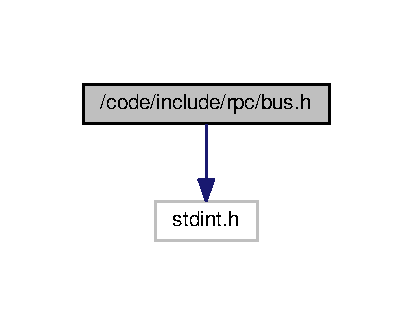
\includegraphics[width=208pt]{bus_8h__incl}
\end{center}
\end{figure}
This graph shows which files directly or indirectly include this file\+:
\nopagebreak
\begin{figure}[H]
\begin{center}
\leavevmode
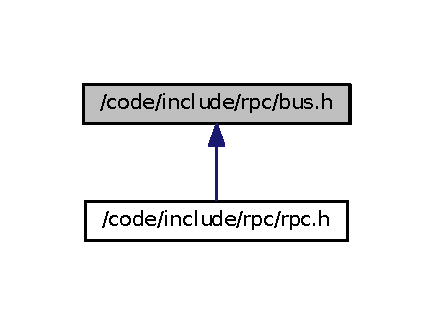
\includegraphics[width=350pt]{bus_8h__dep__incl}
\end{center}
\end{figure}
\subsection*{Classes}
\begin{DoxyCompactItemize}
\item 
struct \hyperlink{structrpc__bus__node}{rpc\+\_\+bus\+\_\+node}
\end{DoxyCompactItemize}
\subsection*{Macros}
\begin{DoxyCompactItemize}
\item 
\#define \hyperlink{bus_8h_aaa8f0d5a3405318f9df38fc2ae8dd587}{R\+P\+C\+\_\+\+B\+U\+S\+\_\+\+E\+V\+E\+N\+T\+\_\+\+H\+A\+N\+D\+L\+ER}(\+\_\+fn,  \+\_\+arg)
\end{DoxyCompactItemize}
\subsection*{Typedefs}
\begin{DoxyCompactItemize}
\item 
typedef void($^\wedge$ \hyperlink{bus_8h_a77cfaa0d7a20750369e9aba0e226a5b5}{rpc\+\_\+bus\+\_\+event\+\_\+handler\+\_\+t}) (\hyperlink{bus_8h_a38a66d3c4093e9ca458510dd2eea7ba7}{rpc\+\_\+bus\+\_\+event\+\_\+t} event, struct \hyperlink{structrpc__bus__node}{rpc\+\_\+bus\+\_\+node} $\ast$\+\_\+\+Nonnull node)
\end{DoxyCompactItemize}
\subsection*{Enumerations}
\begin{DoxyCompactItemize}
\item 
enum \hyperlink{bus_8h_a38a66d3c4093e9ca458510dd2eea7ba7}{rpc\+\_\+bus\+\_\+event\+\_\+t} \{ \hyperlink{bus_8h_a38a66d3c4093e9ca458510dd2eea7ba7a254ff6e09f83f70511fad76529666af5}{R\+P\+C\+\_\+\+B\+U\+S\+\_\+\+A\+T\+T\+A\+C\+H\+ED}, 
\hyperlink{bus_8h_a38a66d3c4093e9ca458510dd2eea7ba7a511c831e9b160756cb2bbcfc587427c6}{R\+P\+C\+\_\+\+B\+U\+S\+\_\+\+D\+E\+T\+A\+C\+H\+ED}
 \}
\end{DoxyCompactItemize}
\subsection*{Functions}
\begin{DoxyCompactItemize}
\item 
int \hyperlink{bus_8h_a845c8c255ac97bb03ac9ad1418eb66f0}{rpc\+\_\+bus\+\_\+open} (void)
\item 
int \hyperlink{bus_8h_a5fa0c254755deec118b2e3dcb4ec9bdf}{rpc\+\_\+bus\+\_\+close} (void)
\item 
int \hyperlink{bus_8h_ac4f30e57bd3b17725db2e517e7cf72a4}{rpc\+\_\+bus\+\_\+ping} (const char $\ast$\+\_\+\+Nonnull serial)
\item 
int \hyperlink{bus_8h_a7dfb66a85e5f3037635a95b693d39a97}{rpc\+\_\+bus\+\_\+enumerate} (struct \hyperlink{structrpc__bus__node}{rpc\+\_\+bus\+\_\+node} $\ast$\+\_\+\+Nullable $\ast$\+\_\+\+Nonnull result)
\item 
void \hyperlink{bus_8h_a7a0ada5e8a9c567b1e7d18297e1cde42}{rpc\+\_\+bus\+\_\+free\+\_\+result} (struct \hyperlink{structrpc__bus__node}{rpc\+\_\+bus\+\_\+node} $\ast$\+\_\+\+Nonnull result)
\item 
void \hyperlink{bus_8h_adbc9a5badea0314236b1ccabb060e090}{rpc\+\_\+bus\+\_\+register\+\_\+event\+\_\+handler} (\+\_\+\+Nonnull \hyperlink{bus_8h_a77cfaa0d7a20750369e9aba0e226a5b5}{rpc\+\_\+bus\+\_\+event\+\_\+handler\+\_\+t} handler)
\item 
void \hyperlink{bus_8h_ae6437acd78bb490baac4517ddffb0792}{rpc\+\_\+bus\+\_\+unregister\+\_\+event\+\_\+handler} (void)
\end{DoxyCompactItemize}


\subsection{Detailed Description}
Bus transport A\+PI 

\subsection{Macro Definition Documentation}
\mbox{\Hypertarget{bus_8h_aaa8f0d5a3405318f9df38fc2ae8dd587}\label{bus_8h_aaa8f0d5a3405318f9df38fc2ae8dd587}} 
\index{bus.\+h@{bus.\+h}!R\+P\+C\+\_\+\+B\+U\+S\+\_\+\+E\+V\+E\+N\+T\+\_\+\+H\+A\+N\+D\+L\+ER@{R\+P\+C\+\_\+\+B\+U\+S\+\_\+\+E\+V\+E\+N\+T\+\_\+\+H\+A\+N\+D\+L\+ER}}
\index{R\+P\+C\+\_\+\+B\+U\+S\+\_\+\+E\+V\+E\+N\+T\+\_\+\+H\+A\+N\+D\+L\+ER@{R\+P\+C\+\_\+\+B\+U\+S\+\_\+\+E\+V\+E\+N\+T\+\_\+\+H\+A\+N\+D\+L\+ER}!bus.\+h@{bus.\+h}}
\subsubsection{\texorpdfstring{R\+P\+C\+\_\+\+B\+U\+S\+\_\+\+E\+V\+E\+N\+T\+\_\+\+H\+A\+N\+D\+L\+ER}{RPC\_BUS\_EVENT\_HANDLER}}
{\footnotesize\ttfamily \#define R\+P\+C\+\_\+\+B\+U\+S\+\_\+\+E\+V\+E\+N\+T\+\_\+\+H\+A\+N\+D\+L\+ER(\begin{DoxyParamCaption}\item[{}]{\+\_\+fn,  }\item[{}]{\+\_\+arg }\end{DoxyParamCaption})}

{\bfseries Value\+:}
\begin{DoxyCode}
^(\hyperlink{bus_8h_a38a66d3c4093e9ca458510dd2eea7ba7}{rpc\_bus\_event\_t} \_event, \textcolor{keyword}{struct }\hyperlink{structrpc__bus__node}{rpc\_bus\_node} *\_node) \{      \(\backslash\)
            \_fn(\_arg, \_event, \_node);                   \(\backslash\)
    \}
\end{DoxyCode}
Converts function pointer to an \hyperlink{bus_8h_a38a66d3c4093e9ca458510dd2eea7ba7}{rpc\+\_\+bus\+\_\+event\+\_\+t} block type. 

Definition at line 73 of file bus.\+h.



\subsection{Typedef Documentation}
\mbox{\Hypertarget{bus_8h_a77cfaa0d7a20750369e9aba0e226a5b5}\label{bus_8h_a77cfaa0d7a20750369e9aba0e226a5b5}} 
\index{bus.\+h@{bus.\+h}!rpc\+\_\+bus\+\_\+event\+\_\+handler\+\_\+t@{rpc\+\_\+bus\+\_\+event\+\_\+handler\+\_\+t}}
\index{rpc\+\_\+bus\+\_\+event\+\_\+handler\+\_\+t@{rpc\+\_\+bus\+\_\+event\+\_\+handler\+\_\+t}!bus.\+h@{bus.\+h}}
\subsubsection{\texorpdfstring{rpc\+\_\+bus\+\_\+event\+\_\+handler\+\_\+t}{rpc\_bus\_event\_handler\_t}}
{\footnotesize\ttfamily typedef void($^\wedge$ rpc\+\_\+bus\+\_\+event\+\_\+handler\+\_\+t) (\hyperlink{bus_8h_a38a66d3c4093e9ca458510dd2eea7ba7}{rpc\+\_\+bus\+\_\+event\+\_\+t} event, struct \hyperlink{structrpc__bus__node}{rpc\+\_\+bus\+\_\+node} $\ast$\+\_\+\+Nonnull node)}

Hotplug event handler callback block type. 

Definition at line 67 of file bus.\+h.



\subsection{Enumeration Type Documentation}
\mbox{\Hypertarget{bus_8h_a38a66d3c4093e9ca458510dd2eea7ba7}\label{bus_8h_a38a66d3c4093e9ca458510dd2eea7ba7}} 
\index{bus.\+h@{bus.\+h}!rpc\+\_\+bus\+\_\+event\+\_\+t@{rpc\+\_\+bus\+\_\+event\+\_\+t}}
\index{rpc\+\_\+bus\+\_\+event\+\_\+t@{rpc\+\_\+bus\+\_\+event\+\_\+t}!bus.\+h@{bus.\+h}}
\subsubsection{\texorpdfstring{rpc\+\_\+bus\+\_\+event\+\_\+t}{rpc\_bus\_event\_t}}
{\footnotesize\ttfamily enum \hyperlink{bus_8h_a38a66d3c4093e9ca458510dd2eea7ba7}{rpc\+\_\+bus\+\_\+event\+\_\+t}}

Bus hot-\/plug event type. \begin{DoxyEnumFields}{Enumerator}
\raisebox{\heightof{T}}[0pt][0pt]{\index{R\+P\+C\+\_\+\+B\+U\+S\+\_\+\+A\+T\+T\+A\+C\+H\+ED@{R\+P\+C\+\_\+\+B\+U\+S\+\_\+\+A\+T\+T\+A\+C\+H\+ED}!bus.\+h@{bus.\+h}}\index{bus.\+h@{bus.\+h}!R\+P\+C\+\_\+\+B\+U\+S\+\_\+\+A\+T\+T\+A\+C\+H\+ED@{R\+P\+C\+\_\+\+B\+U\+S\+\_\+\+A\+T\+T\+A\+C\+H\+ED}}}\mbox{\Hypertarget{bus_8h_a38a66d3c4093e9ca458510dd2eea7ba7a254ff6e09f83f70511fad76529666af5}\label{bus_8h_a38a66d3c4093e9ca458510dd2eea7ba7a254ff6e09f83f70511fad76529666af5}} 
R\+P\+C\+\_\+\+B\+U\+S\+\_\+\+A\+T\+T\+A\+C\+H\+ED&Device attached to the system \\
\hline

\raisebox{\heightof{T}}[0pt][0pt]{\index{R\+P\+C\+\_\+\+B\+U\+S\+\_\+\+D\+E\+T\+A\+C\+H\+ED@{R\+P\+C\+\_\+\+B\+U\+S\+\_\+\+D\+E\+T\+A\+C\+H\+ED}!bus.\+h@{bus.\+h}}\index{bus.\+h@{bus.\+h}!R\+P\+C\+\_\+\+B\+U\+S\+\_\+\+D\+E\+T\+A\+C\+H\+ED@{R\+P\+C\+\_\+\+B\+U\+S\+\_\+\+D\+E\+T\+A\+C\+H\+ED}}}\mbox{\Hypertarget{bus_8h_a38a66d3c4093e9ca458510dd2eea7ba7a511c831e9b160756cb2bbcfc587427c6}\label{bus_8h_a38a66d3c4093e9ca458510dd2eea7ba7a511c831e9b160756cb2bbcfc587427c6}} 
R\+P\+C\+\_\+\+B\+U\+S\+\_\+\+D\+E\+T\+A\+C\+H\+ED&Device detached from the system \\
\hline

\end{DoxyEnumFields}


Definition at line 45 of file bus.\+h.



\subsection{Function Documentation}
\mbox{\Hypertarget{bus_8h_a5fa0c254755deec118b2e3dcb4ec9bdf}\label{bus_8h_a5fa0c254755deec118b2e3dcb4ec9bdf}} 
\index{bus.\+h@{bus.\+h}!rpc\+\_\+bus\+\_\+close@{rpc\+\_\+bus\+\_\+close}}
\index{rpc\+\_\+bus\+\_\+close@{rpc\+\_\+bus\+\_\+close}!bus.\+h@{bus.\+h}}
\subsubsection{\texorpdfstring{rpc\+\_\+bus\+\_\+close()}{rpc\_bus\_close()}}
{\footnotesize\ttfamily int rpc\+\_\+bus\+\_\+close (\begin{DoxyParamCaption}\item[{void}]{ }\end{DoxyParamCaption})}

Closes the librpc bus connection.

\begin{DoxyReturn}{Returns}
0 on success, -\/1 on error 
\end{DoxyReturn}
\begin{Desc}
\item[Examples\+: ]\par
\hyperlink{bus_8c-example}{bus.\+c}.\end{Desc}
\mbox{\Hypertarget{bus_8h_a7dfb66a85e5f3037635a95b693d39a97}\label{bus_8h_a7dfb66a85e5f3037635a95b693d39a97}} 
\index{bus.\+h@{bus.\+h}!rpc\+\_\+bus\+\_\+enumerate@{rpc\+\_\+bus\+\_\+enumerate}}
\index{rpc\+\_\+bus\+\_\+enumerate@{rpc\+\_\+bus\+\_\+enumerate}!bus.\+h@{bus.\+h}}
\subsubsection{\texorpdfstring{rpc\+\_\+bus\+\_\+enumerate()}{rpc\_bus\_enumerate()}}
{\footnotesize\ttfamily int rpc\+\_\+bus\+\_\+enumerate (\begin{DoxyParamCaption}\item[{struct \hyperlink{structrpc__bus__node}{rpc\+\_\+bus\+\_\+node} $\ast$\+\_\+\+Nullable $\ast$\+\_\+\+Nonnull}]{result }\end{DoxyParamCaption})}

Enumerates connected devices on the R\+PC bus.


\begin{DoxyParams}{Parameters}
{\em result} & Array of \hyperlink{structrpc__bus__node}{rpc\+\_\+bus\+\_\+node} elements \\
\hline
\end{DoxyParams}
\begin{DoxyReturn}{Returns}
0 on success, -\/1 on error 
\end{DoxyReturn}
\begin{Desc}
\item[Examples\+: ]\par
\hyperlink{bus_8c-example}{bus.\+c}.\end{Desc}
\mbox{\Hypertarget{bus_8h_a7a0ada5e8a9c567b1e7d18297e1cde42}\label{bus_8h_a7a0ada5e8a9c567b1e7d18297e1cde42}} 
\index{bus.\+h@{bus.\+h}!rpc\+\_\+bus\+\_\+free\+\_\+result@{rpc\+\_\+bus\+\_\+free\+\_\+result}}
\index{rpc\+\_\+bus\+\_\+free\+\_\+result@{rpc\+\_\+bus\+\_\+free\+\_\+result}!bus.\+h@{bus.\+h}}
\subsubsection{\texorpdfstring{rpc\+\_\+bus\+\_\+free\+\_\+result()}{rpc\_bus\_free\_result()}}
{\footnotesize\ttfamily void rpc\+\_\+bus\+\_\+free\+\_\+result (\begin{DoxyParamCaption}\item[{struct \hyperlink{structrpc__bus__node}{rpc\+\_\+bus\+\_\+node} $\ast$\+\_\+\+Nonnull}]{result }\end{DoxyParamCaption})}

Frees struct \hyperlink{structrpc__bus__node}{rpc\+\_\+bus\+\_\+node} array obtained in \hyperlink{bus_8h_a7dfb66a85e5f3037635a95b693d39a97}{rpc\+\_\+bus\+\_\+enumerate} call.


\begin{DoxyParams}{Parameters}
{\em result} & Array of struct \hyperlink{structrpc__bus__node}{rpc\+\_\+bus\+\_\+node} elements \\
\hline
\end{DoxyParams}
\begin{Desc}
\item[Examples\+: ]\par
\hyperlink{bus_8c-example}{bus.\+c}.\end{Desc}
\mbox{\Hypertarget{bus_8h_a845c8c255ac97bb03ac9ad1418eb66f0}\label{bus_8h_a845c8c255ac97bb03ac9ad1418eb66f0}} 
\index{bus.\+h@{bus.\+h}!rpc\+\_\+bus\+\_\+open@{rpc\+\_\+bus\+\_\+open}}
\index{rpc\+\_\+bus\+\_\+open@{rpc\+\_\+bus\+\_\+open}!bus.\+h@{bus.\+h}}
\subsubsection{\texorpdfstring{rpc\+\_\+bus\+\_\+open()}{rpc\_bus\_open()}}
{\footnotesize\ttfamily int rpc\+\_\+bus\+\_\+open (\begin{DoxyParamCaption}\item[{void}]{ }\end{DoxyParamCaption})}

Opens the librpc bus connection.

\begin{DoxyReturn}{Returns}
0 on success, -\/1 on error 
\end{DoxyReturn}
\begin{Desc}
\item[Examples\+: ]\par
\hyperlink{bus_8c-example}{bus.\+c}.\end{Desc}
\mbox{\Hypertarget{bus_8h_ac4f30e57bd3b17725db2e517e7cf72a4}\label{bus_8h_ac4f30e57bd3b17725db2e517e7cf72a4}} 
\index{bus.\+h@{bus.\+h}!rpc\+\_\+bus\+\_\+ping@{rpc\+\_\+bus\+\_\+ping}}
\index{rpc\+\_\+bus\+\_\+ping@{rpc\+\_\+bus\+\_\+ping}!bus.\+h@{bus.\+h}}
\subsubsection{\texorpdfstring{rpc\+\_\+bus\+\_\+ping()}{rpc\_bus\_ping()}}
{\footnotesize\ttfamily int rpc\+\_\+bus\+\_\+ping (\begin{DoxyParamCaption}\item[{const char $\ast$\+\_\+\+Nonnull}]{serial }\end{DoxyParamCaption})}

Checks whether a node with specified serial is reachable.


\begin{DoxyParams}{Parameters}
{\em serial} & Node serial number \\
\hline
\end{DoxyParams}
\begin{DoxyReturn}{Returns}
0 if reachable, -\/1 otherwise 
\end{DoxyReturn}
\begin{Desc}
\item[Examples\+: ]\par
\hyperlink{bus_8c-example}{bus.\+c}.\end{Desc}
\mbox{\Hypertarget{bus_8h_adbc9a5badea0314236b1ccabb060e090}\label{bus_8h_adbc9a5badea0314236b1ccabb060e090}} 
\index{bus.\+h@{bus.\+h}!rpc\+\_\+bus\+\_\+register\+\_\+event\+\_\+handler@{rpc\+\_\+bus\+\_\+register\+\_\+event\+\_\+handler}}
\index{rpc\+\_\+bus\+\_\+register\+\_\+event\+\_\+handler@{rpc\+\_\+bus\+\_\+register\+\_\+event\+\_\+handler}!bus.\+h@{bus.\+h}}
\subsubsection{\texorpdfstring{rpc\+\_\+bus\+\_\+register\+\_\+event\+\_\+handler()}{rpc\_bus\_register\_event\_handler()}}
{\footnotesize\ttfamily void rpc\+\_\+bus\+\_\+register\+\_\+event\+\_\+handler (\begin{DoxyParamCaption}\item[{\+\_\+\+Nonnull \hyperlink{bus_8h_a77cfaa0d7a20750369e9aba0e226a5b5}{rpc\+\_\+bus\+\_\+event\+\_\+handler\+\_\+t}}]{handler }\end{DoxyParamCaption})}

Configures an event handler block to be called whenever a bus event occurs.


\begin{DoxyParams}{Parameters}
{\em handler} & Bus event handler \\
\hline
\end{DoxyParams}
\mbox{\Hypertarget{bus_8h_ae6437acd78bb490baac4517ddffb0792}\label{bus_8h_ae6437acd78bb490baac4517ddffb0792}} 
\index{bus.\+h@{bus.\+h}!rpc\+\_\+bus\+\_\+unregister\+\_\+event\+\_\+handler@{rpc\+\_\+bus\+\_\+unregister\+\_\+event\+\_\+handler}}
\index{rpc\+\_\+bus\+\_\+unregister\+\_\+event\+\_\+handler@{rpc\+\_\+bus\+\_\+unregister\+\_\+event\+\_\+handler}!bus.\+h@{bus.\+h}}
\subsubsection{\texorpdfstring{rpc\+\_\+bus\+\_\+unregister\+\_\+event\+\_\+handler()}{rpc\_bus\_unregister\_event\_handler()}}
{\footnotesize\ttfamily void rpc\+\_\+bus\+\_\+unregister\+\_\+event\+\_\+handler (\begin{DoxyParamCaption}\item[{void}]{ }\end{DoxyParamCaption})}

Unsets the previously set event handler. If there was no handler previously configured, does nothing. 
\hypertarget{client_8h}{\section{/home/travis/build/twoporeguys/librpc/include/rpc/client.h File Reference}
\label{client_8h}\index{/home/travis/build/twoporeguys/librpc/include/rpc/client.\-h@{/home/travis/build/twoporeguys/librpc/include/rpc/client.\-h}}
}
{\ttfamily \#include $<$stdbool.\-h$>$}\\*
{\ttfamily \#include $<$rpc/connection.\-h$>$}\\*
Include dependency graph for client.\-h\-:
\nopagebreak
\begin{figure}[H]
\begin{center}
\leavevmode
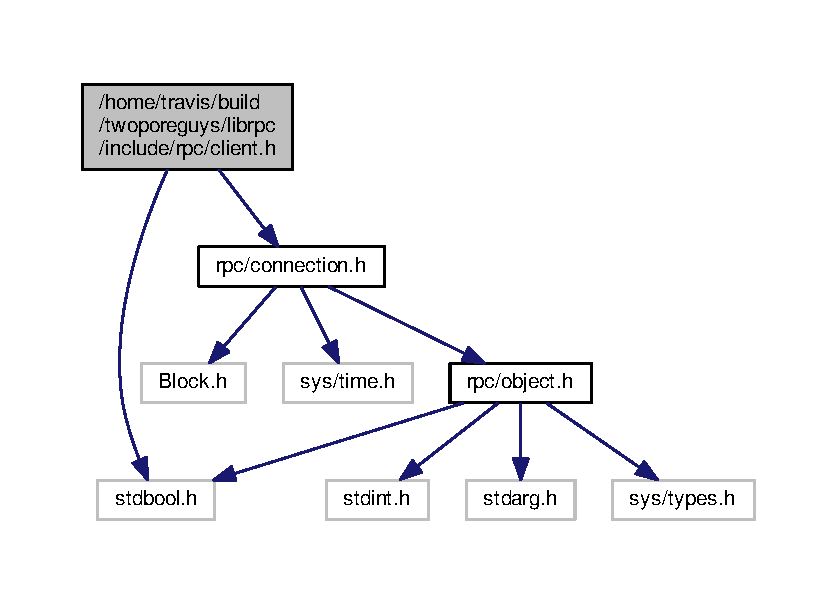
\includegraphics[width=350pt]{client_8h__incl}
\end{center}
\end{figure}
\subsection*{Typedefs}
\begin{DoxyCompactItemize}
\item 
\hypertarget{client_8h_a4f7230a0c2c07d27a07a88d407a06b70}{typedef struct rpc\-\_\-client $\ast$ {\bfseries rpc\-\_\-client\-\_\-t}}\label{client_8h_a4f7230a0c2c07d27a07a88d407a06b70}

\end{DoxyCompactItemize}
\subsection*{Functions}
\begin{DoxyCompactItemize}
\item 
rpc\-\_\-client\-\_\-t \hyperlink{client_8h_aa2ee510504eb2546129fd29733666c34}{rpc\-\_\-client\-\_\-create} (const char $\ast$uri, int flags)
\item 
rpc\-\_\-connection\-\_\-t \hyperlink{client_8h_a115d9a7fa40d9ec52a2fb553426fc202}{rpc\-\_\-client\-\_\-get\-\_\-connection} (rpc\-\_\-client\-\_\-t client)
\item 
void \hyperlink{client_8h_ababbc19eeaefeab208c5b6d80411ee77}{rpc\-\_\-client\-\_\-close} (rpc\-\_\-client\-\_\-t client)
\end{DoxyCompactItemize}


\subsection{Detailed Description}
R\-P\-C client A\-P\-I. 

Definition in file \hyperlink{client_8h_source}{client.\-h}.



\subsection{Function Documentation}
\hypertarget{client_8h_ababbc19eeaefeab208c5b6d80411ee77}{\index{client.\-h@{client.\-h}!rpc\-\_\-client\-\_\-close@{rpc\-\_\-client\-\_\-close}}
\index{rpc\-\_\-client\-\_\-close@{rpc\-\_\-client\-\_\-close}!client.h@{client.\-h}}
\subsubsection[{rpc\-\_\-client\-\_\-close}]{\setlength{\rightskip}{0pt plus 5cm}void rpc\-\_\-client\-\_\-close (
\begin{DoxyParamCaption}
\item[{rpc\-\_\-client\-\_\-t}]{client}
\end{DoxyParamCaption}
)}}\label{client_8h_ababbc19eeaefeab208c5b6d80411ee77}
Closes the connection and frees associated resources.


\begin{DoxyParams}{Parameters}
{\em client} & Client object \\
\hline
\end{DoxyParams}
\hypertarget{client_8h_aa2ee510504eb2546129fd29733666c34}{\index{client.\-h@{client.\-h}!rpc\-\_\-client\-\_\-create@{rpc\-\_\-client\-\_\-create}}
\index{rpc\-\_\-client\-\_\-create@{rpc\-\_\-client\-\_\-create}!client.h@{client.\-h}}
\subsubsection[{rpc\-\_\-client\-\_\-create}]{\setlength{\rightskip}{0pt plus 5cm}rpc\-\_\-client\-\_\-t rpc\-\_\-client\-\_\-create (
\begin{DoxyParamCaption}
\item[{const char $\ast$}]{uri, }
\item[{int}]{flags}
\end{DoxyParamCaption}
)}}\label{client_8h_aa2ee510504eb2546129fd29733666c34}
Creates a new, connected R\-P\-C client.

U\-R\-I parameter can take multiple forms\-:
\begin{DoxyItemize}
\item unix\-://$<$path$>$ connects to an Unix domain socket
\item tcp\-://$<$ip-\/address$>$\-:$<$port$>$ connects using a T\-C\-P socket
\item ws\-://$<$ip-\/address$>$\-:$<$port$>$/$<$path$>$ connects using a Web\-Socket
\item loopback\-://$<$id$>$ connects using a local transport
\end{DoxyItemize}


\begin{DoxyParams}{Parameters}
{\em uri} & Endpoint U\-R\-I \\
\hline
{\em flags} & Currently unused \\
\hline
\end{DoxyParams}
\begin{DoxyReturn}{Returns}
Connect R\-P\-C client object 
\end{DoxyReturn}
\hypertarget{client_8h_a115d9a7fa40d9ec52a2fb553426fc202}{\index{client.\-h@{client.\-h}!rpc\-\_\-client\-\_\-get\-\_\-connection@{rpc\-\_\-client\-\_\-get\-\_\-connection}}
\index{rpc\-\_\-client\-\_\-get\-\_\-connection@{rpc\-\_\-client\-\_\-get\-\_\-connection}!client.h@{client.\-h}}
\subsubsection[{rpc\-\_\-client\-\_\-get\-\_\-connection}]{\setlength{\rightskip}{0pt plus 5cm}rpc\-\_\-connection\-\_\-t rpc\-\_\-client\-\_\-get\-\_\-connection (
\begin{DoxyParamCaption}
\item[{rpc\-\_\-client\-\_\-t}]{client}
\end{DoxyParamCaption}
)}}\label{client_8h_a115d9a7fa40d9ec52a2fb553426fc202}
Gets the connection object from a client.


\begin{DoxyParams}{Parameters}
{\em client} & Client object to get the connection from \\
\hline
\end{DoxyParams}
\begin{DoxyReturn}{Returns}
Connection object 
\end{DoxyReturn}

\hypertarget{connection_8h}{}\section{/code/include/rpc/connection.h File Reference}
\label{connection_8h}\index{/code/include/rpc/connection.\+h@{/code/include/rpc/connection.\+h}}
{\ttfamily \#include $<$Block.\+h$>$}\\*
{\ttfamily \#include $<$sys/time.\+h$>$}\\*
{\ttfamily \#include $<$rpc/object.\+h$>$}\\*
Include dependency graph for connection.\+h\+:
\nopagebreak
\begin{figure}[H]
\begin{center}
\leavevmode
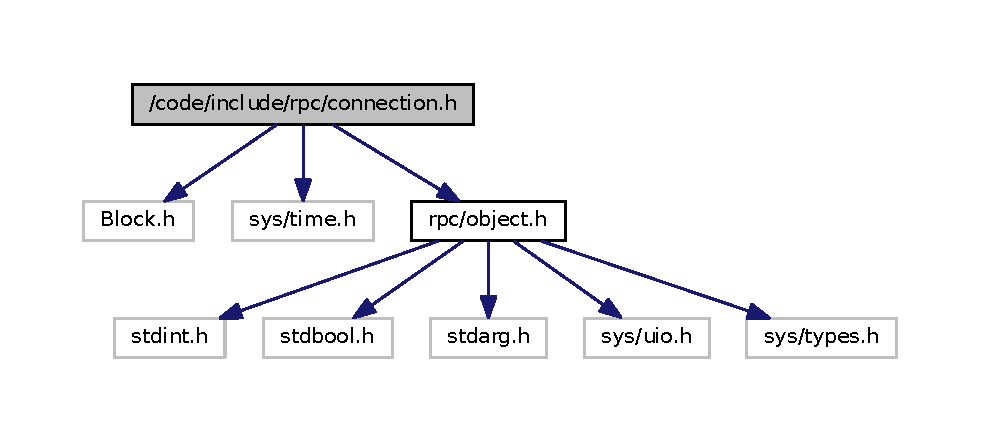
\includegraphics[width=350pt]{connection_8h__incl}
\end{center}
\end{figure}
This graph shows which files directly or indirectly include this file\+:
\nopagebreak
\begin{figure}[H]
\begin{center}
\leavevmode
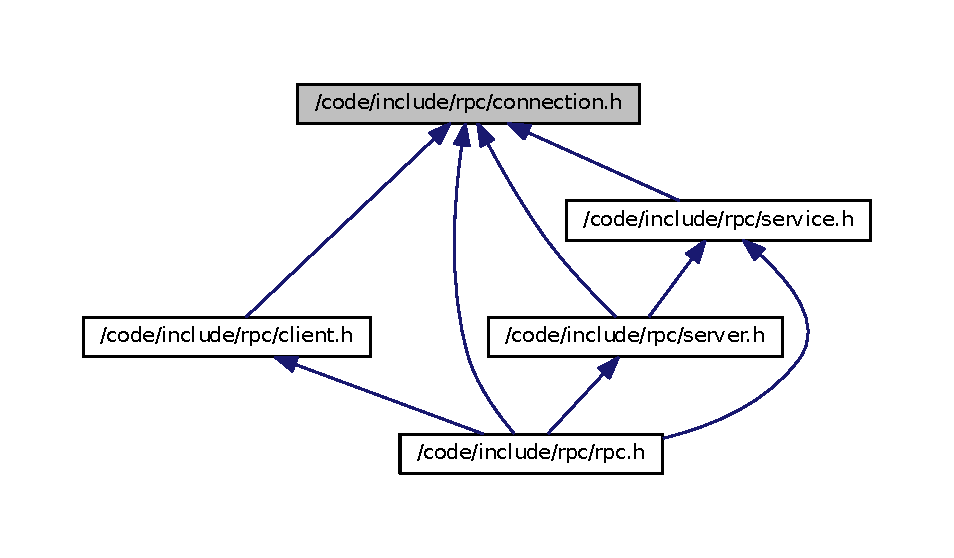
\includegraphics[width=350pt]{connection_8h__dep__incl}
\end{center}
\end{figure}
\subsection*{Macros}
\begin{DoxyCompactItemize}
\item 
\#define \hyperlink{connection_8h_a4f7704822a76a6f293f6abbb59bf41f3}{R\+P\+C\+\_\+\+H\+A\+N\+D\+L\+ER}(\+\_\+fn,  \+\_\+arg)
\item 
\#define \hyperlink{connection_8h_ac6630daf34229f9dd8a754b119e4a94d}{R\+P\+C\+\_\+\+E\+R\+R\+O\+R\+\_\+\+H\+A\+N\+D\+L\+ER}(\+\_\+fn,  \+\_\+arg)
\item 
\#define \hyperlink{connection_8h_a7512dc753949d75650bbec7527f9d0a6}{R\+P\+C\+\_\+\+C\+A\+L\+L\+B\+A\+CK}(\+\_\+fn,  \+\_\+arg)
\end{DoxyCompactItemize}
\subsection*{Typedefs}
\begin{DoxyCompactItemize}
\item 
typedef enum \hyperlink{connection_8h_a88bd06a910a4ce0b9046b9beb4af5ccd}{rpc\+\_\+error\+\_\+code} \hyperlink{connection_8h_a043170f29cb25827a88be4dab2313a91}{rpc\+\_\+error\+\_\+code\+\_\+t}
\item 
typedef enum \hyperlink{connection_8h_a22306445a7503bab94835382d07e0410}{rpc\+\_\+call\+\_\+status} \hyperlink{connection_8h_a5e44285dc90be1f6bc541504a3f6d929}{rpc\+\_\+call\+\_\+status\+\_\+t}
\item 
typedef struct rpc\+\_\+connection $\ast$ \hyperlink{connection_8h_a70838cb106c3464db299522c5fe2782d}{rpc\+\_\+connection\+\_\+t}
\item 
typedef struct rpc\+\_\+call $\ast$ \hyperlink{connection_8h_aeb6f25e395cc04930537960ef6b50106}{rpc\+\_\+call\+\_\+t}
\item 
typedef void($^\wedge$ \hyperlink{connection_8h_ae18f6c0163bc8460cee1b6332c83fe07}{rpc\+\_\+handler\+\_\+t}) (const char $\ast$path, const char $\ast$interface, const char $\ast$name, \hyperlink{object_8h_ab365f726b4975c0c8376b808d111d01b}{rpc\+\_\+object\+\_\+t} args)
\item 
typedef void($^\wedge$ \hyperlink{connection_8h_a4dfba30ff97d4c5c56a6787ecd1bb79a}{rpc\+\_\+error\+\_\+handler\+\_\+t}) (\hyperlink{connection_8h_a043170f29cb25827a88be4dab2313a91}{rpc\+\_\+error\+\_\+code\+\_\+t} code, \hyperlink{object_8h_ab365f726b4975c0c8376b808d111d01b}{rpc\+\_\+object\+\_\+t} args)
\item 
typedef bool($^\wedge$ \hyperlink{connection_8h_a659dfc386fa0add62a07c17662a29641}{rpc\+\_\+callback\+\_\+t}) (\hyperlink{object_8h_ab365f726b4975c0c8376b808d111d01b}{rpc\+\_\+object\+\_\+t} args, \hyperlink{connection_8h_a5e44285dc90be1f6bc541504a3f6d929}{rpc\+\_\+call\+\_\+status\+\_\+t} status)
\end{DoxyCompactItemize}
\subsection*{Enumerations}
\begin{DoxyCompactItemize}
\item 
enum \hyperlink{connection_8h_a88bd06a910a4ce0b9046b9beb4af5ccd}{rpc\+\_\+error\+\_\+code} \{ \\*
\hyperlink{connection_8h_a88bd06a910a4ce0b9046b9beb4af5ccda675a64c636ef92f53c398f7cf1e7b4f7}{R\+P\+C\+\_\+\+I\+N\+V\+A\+L\+I\+D\+\_\+\+R\+E\+S\+P\+O\+N\+SE} = 1, 
\hyperlink{connection_8h_a88bd06a910a4ce0b9046b9beb4af5ccda68a960230d093e43260efb62951a6d55}{R\+P\+C\+\_\+\+C\+O\+N\+N\+E\+C\+T\+I\+O\+N\+\_\+\+T\+I\+M\+E\+O\+UT}, 
\hyperlink{connection_8h_a88bd06a910a4ce0b9046b9beb4af5ccdab6000475e99b77735aac87708b4aacb0}{R\+P\+C\+\_\+\+C\+O\+N\+N\+E\+C\+T\+I\+O\+N\+\_\+\+C\+L\+O\+S\+ED}, 
\hyperlink{connection_8h_a88bd06a910a4ce0b9046b9beb4af5ccda51853f66b918b83f313c330c02452c70}{R\+P\+C\+\_\+\+C\+A\+L\+L\+\_\+\+T\+I\+M\+E\+O\+UT}, 
\\*
\hyperlink{connection_8h_a88bd06a910a4ce0b9046b9beb4af5ccda8efbac3939ec6e713c533b113ebb741d}{R\+P\+C\+\_\+\+S\+P\+U\+R\+I\+O\+U\+S\+\_\+\+R\+E\+S\+P\+O\+N\+SE}, 
\hyperlink{connection_8h_a88bd06a910a4ce0b9046b9beb4af5ccda27f60e17ed6dc1019e2beec97e597c9b}{R\+P\+C\+\_\+\+L\+O\+G\+O\+UT}, 
\hyperlink{connection_8h_a88bd06a910a4ce0b9046b9beb4af5ccda90324cd01756fadc8e9784079af790c1}{R\+P\+C\+\_\+\+O\+T\+H\+ER}
 \}
\item 
enum \hyperlink{connection_8h_a22306445a7503bab94835382d07e0410}{rpc\+\_\+call\+\_\+status} \{ \\*
\hyperlink{connection_8h_a22306445a7503bab94835382d07e0410a1773d93b43fed839dc871589691fdef1}{R\+P\+C\+\_\+\+C\+A\+L\+L\+\_\+\+I\+N\+\_\+\+P\+R\+O\+G\+R\+E\+SS}, 
\hyperlink{connection_8h_a22306445a7503bab94835382d07e0410ab6194e76e0430da03cedbe2541889e6f}{R\+P\+C\+\_\+\+C\+A\+L\+L\+\_\+\+M\+O\+R\+E\+\_\+\+A\+V\+A\+I\+L\+A\+B\+LE}, 
\hyperlink{connection_8h_a22306445a7503bab94835382d07e0410a251c1dd2588db7249fc6321f8be6988d}{R\+P\+C\+\_\+\+C\+A\+L\+L\+\_\+\+D\+O\+NE}, 
\hyperlink{connection_8h_a22306445a7503bab94835382d07e0410aa86df1455d84a8c7c3b4f918cb626856}{R\+P\+C\+\_\+\+C\+A\+L\+L\+\_\+\+E\+R\+R\+OR}, 
\\*
\hyperlink{connection_8h_a22306445a7503bab94835382d07e0410a6c33a14b8aa6d0797cb614b890e9c741}{R\+P\+C\+\_\+\+C\+A\+L\+L\+\_\+\+A\+B\+O\+R\+T\+ED}
 \}
\end{DoxyCompactItemize}
\subsection*{Functions}
\begin{DoxyCompactItemize}
\item 
\hyperlink{connection_8h_a70838cb106c3464db299522c5fe2782d}{rpc\+\_\+connection\+\_\+t} {\bfseries rpc\+\_\+connection\+\_\+create} (void $\ast$cookie, \hyperlink{object_8h_ab365f726b4975c0c8376b808d111d01b}{rpc\+\_\+object\+\_\+t} params)\hypertarget{connection_8h_a0382631023d9cf812d978e80d5814bc8}{}\label{connection_8h_a0382631023d9cf812d978e80d5814bc8}

\item 
int \hyperlink{connection_8h_a6d4de49f4d9121c4077e62b73064b99d}{rpc\+\_\+connection\+\_\+close} (\hyperlink{connection_8h_a70838cb106c3464db299522c5fe2782d}{rpc\+\_\+connection\+\_\+t} conn)
\item 
int \hyperlink{connection_8h_ae9e20b8d59848a4124c4150be552c623}{rpc\+\_\+connection\+\_\+subscribe\+\_\+event} (\hyperlink{connection_8h_a70838cb106c3464db299522c5fe2782d}{rpc\+\_\+connection\+\_\+t} conn, const char $\ast$path, const char $\ast$interface, const char $\ast$name)
\item 
int \hyperlink{connection_8h_a52a9651ed03823775ef6bb8716f1db03}{rpc\+\_\+connection\+\_\+unsubscribe\+\_\+event} (\hyperlink{connection_8h_a70838cb106c3464db299522c5fe2782d}{rpc\+\_\+connection\+\_\+t} conn, const char $\ast$path, const char $\ast$interface, const char $\ast$name)
\item 
void $\ast$ \hyperlink{connection_8h_a2d2006058675a9f55c48a116790132c8}{rpc\+\_\+connection\+\_\+register\+\_\+event\+\_\+handler} (\hyperlink{connection_8h_a70838cb106c3464db299522c5fe2782d}{rpc\+\_\+connection\+\_\+t} conn, const char $\ast$path, const char $\ast$interface, const char $\ast$name, \hyperlink{connection_8h_ae18f6c0163bc8460cee1b6332c83fe07}{rpc\+\_\+handler\+\_\+t} handler)
\item 
void \hyperlink{connection_8h_a8174aa9225c291138d5f409a1089f6cc}{rpc\+\_\+connection\+\_\+unregister\+\_\+event\+\_\+handler} (\hyperlink{connection_8h_a70838cb106c3464db299522c5fe2782d}{rpc\+\_\+connection\+\_\+t} conn, void $\ast$cookie)
\item 
\hyperlink{object_8h_ab365f726b4975c0c8376b808d111d01b}{rpc\+\_\+object\+\_\+t} \hyperlink{connection_8h_a4bb388f7cc19ce3d01577993fcf7dd63}{rpc\+\_\+connection\+\_\+call\+\_\+sync} (\hyperlink{connection_8h_a70838cb106c3464db299522c5fe2782d}{rpc\+\_\+connection\+\_\+t} conn, const char $\ast$path, const char $\ast$interface, const char $\ast$method,...)
\item 
\hyperlink{object_8h_ab365f726b4975c0c8376b808d111d01b}{rpc\+\_\+object\+\_\+t} \hyperlink{connection_8h_a62df11aec4a738cc80defd3408354721}{rpc\+\_\+connection\+\_\+call\+\_\+syncv} (\hyperlink{connection_8h_a70838cb106c3464db299522c5fe2782d}{rpc\+\_\+connection\+\_\+t} conn, const char $\ast$path, const char $\ast$interface, const char $\ast$method, va\+\_\+list ap)
\item 
\hyperlink{object_8h_ab365f726b4975c0c8376b808d111d01b}{rpc\+\_\+object\+\_\+t} \hyperlink{connection_8h_a0bbf25b18122ee854bc8f0016bc84eeb}{rpc\+\_\+connection\+\_\+call\+\_\+syncp} (\hyperlink{connection_8h_a70838cb106c3464db299522c5fe2782d}{rpc\+\_\+connection\+\_\+t} conn, const char $\ast$path, const char $\ast$interface, const char $\ast$method, const char $\ast$fmt,...)
\item 
\hyperlink{object_8h_ab365f726b4975c0c8376b808d111d01b}{rpc\+\_\+object\+\_\+t} \hyperlink{connection_8h_a0528a5ec56934aa35e9c51423b54c880}{rpc\+\_\+connection\+\_\+call\+\_\+syncpv} (\hyperlink{connection_8h_a70838cb106c3464db299522c5fe2782d}{rpc\+\_\+connection\+\_\+t} conn, const char $\ast$path, const char $\ast$interface, const char $\ast$method, const char $\ast$fmt, va\+\_\+list ap)
\item 
\hyperlink{object_8h_ab365f726b4975c0c8376b808d111d01b}{rpc\+\_\+object\+\_\+t} \hyperlink{connection_8h_a308c17c19fccdd57ae46739b860aea19}{rpc\+\_\+connection\+\_\+call\+\_\+simple} (\hyperlink{connection_8h_a70838cb106c3464db299522c5fe2782d}{rpc\+\_\+connection\+\_\+t} conn, const char $\ast$name, const char $\ast$fmt,...)
\item 
\hyperlink{connection_8h_aeb6f25e395cc04930537960ef6b50106}{rpc\+\_\+call\+\_\+t} \hyperlink{connection_8h_a2d2059a4a18c0bfb8d8482af47d34072}{rpc\+\_\+connection\+\_\+call} (\hyperlink{connection_8h_a70838cb106c3464db299522c5fe2782d}{rpc\+\_\+connection\+\_\+t} conn, const char $\ast$path, const char $\ast$interface, const char $\ast$name, \hyperlink{object_8h_ab365f726b4975c0c8376b808d111d01b}{rpc\+\_\+object\+\_\+t} args, \hyperlink{connection_8h_a659dfc386fa0add62a07c17662a29641}{rpc\+\_\+callback\+\_\+t} callback)
\item 
\hyperlink{object_8h_ab365f726b4975c0c8376b808d111d01b}{rpc\+\_\+object\+\_\+t} \hyperlink{connection_8h_a87b152a8ef73a75ac770a74283e05dc8}{rpc\+\_\+connection\+\_\+get\+\_\+property} (\hyperlink{connection_8h_a70838cb106c3464db299522c5fe2782d}{rpc\+\_\+connection\+\_\+t} conn, const char $\ast$path, const char $\ast$interface, const char $\ast$name)
\item 
\hyperlink{object_8h_ab365f726b4975c0c8376b808d111d01b}{rpc\+\_\+object\+\_\+t} \hyperlink{connection_8h_a6fa1783ffe617c0c0342d365ad9c28fa}{rpc\+\_\+connection\+\_\+set\+\_\+property} (\hyperlink{connection_8h_a70838cb106c3464db299522c5fe2782d}{rpc\+\_\+connection\+\_\+t} conn, const char $\ast$path, const char $\ast$interface, const char $\ast$name, \hyperlink{object_8h_ab365f726b4975c0c8376b808d111d01b}{rpc\+\_\+object\+\_\+t} value)
\item 
\hyperlink{object_8h_ab365f726b4975c0c8376b808d111d01b}{rpc\+\_\+object\+\_\+t} \hyperlink{connection_8h_aae34b6e1d7bffb1d6af187b1d893affa}{rpc\+\_\+connection\+\_\+set\+\_\+propertyp} (\hyperlink{connection_8h_a70838cb106c3464db299522c5fe2782d}{rpc\+\_\+connection\+\_\+t} conn, const char $\ast$path, const char $\ast$interface, const char $\ast$name, const char $\ast$fmt,...)
\item 
\hyperlink{object_8h_ab365f726b4975c0c8376b808d111d01b}{rpc\+\_\+object\+\_\+t} \hyperlink{connection_8h_aede502dc903184162fbe144c6a29968f}{rpc\+\_\+connection\+\_\+set\+\_\+propertypv} (\hyperlink{connection_8h_a70838cb106c3464db299522c5fe2782d}{rpc\+\_\+connection\+\_\+t} conn, const char $\ast$path, const char $\ast$interface, const char $\ast$name, const char $\ast$fmt, va\+\_\+list ap)
\item 
int \hyperlink{connection_8h_a4fe29725255d1cbfcfec6e719e7023df}{rpc\+\_\+connection\+\_\+send\+\_\+event} (\hyperlink{connection_8h_a70838cb106c3464db299522c5fe2782d}{rpc\+\_\+connection\+\_\+t} conn, const char $\ast$path, const char $\ast$interface, const char $\ast$name, \hyperlink{object_8h_ab365f726b4975c0c8376b808d111d01b}{rpc\+\_\+object\+\_\+t} args)
\item 
int \hyperlink{connection_8h_a2d9343c2c38625f9659358e0710ed0c7}{rpc\+\_\+connection\+\_\+ping} (\hyperlink{connection_8h_a70838cb106c3464db299522c5fe2782d}{rpc\+\_\+connection\+\_\+t} conn)
\item 
void \hyperlink{connection_8h_ae843166183a4bd6dbf5a58133b3fcaf3}{rpc\+\_\+connection\+\_\+set\+\_\+event\+\_\+handler} (\hyperlink{connection_8h_a70838cb106c3464db299522c5fe2782d}{rpc\+\_\+connection\+\_\+t} conn, \hyperlink{connection_8h_ae18f6c0163bc8460cee1b6332c83fe07}{rpc\+\_\+handler\+\_\+t} handler)
\item 
void \hyperlink{connection_8h_a8f332abcc5d0a80c86f8317c7dcc79ec}{rpc\+\_\+connection\+\_\+set\+\_\+error\+\_\+handler} (\hyperlink{connection_8h_a70838cb106c3464db299522c5fe2782d}{rpc\+\_\+connection\+\_\+t} conn, \hyperlink{connection_8h_a4dfba30ff97d4c5c56a6787ecd1bb79a}{rpc\+\_\+error\+\_\+handler\+\_\+t} handler)
\item 
const char $\ast$ \hyperlink{connection_8h_af8da8ac07f9e61dec2f9159032c4edf3}{rpc\+\_\+connection\+\_\+get\+\_\+remote\+\_\+address} (\hyperlink{connection_8h_a70838cb106c3464db299522c5fe2782d}{rpc\+\_\+connection\+\_\+t} conn)
\item 
bool \hyperlink{connection_8h_a581a8e0a711f89b5d41982fbd920561f}{rpc\+\_\+connection\+\_\+has\+\_\+credentials} (\hyperlink{connection_8h_a70838cb106c3464db299522c5fe2782d}{rpc\+\_\+connection\+\_\+t} conn)
\item 
uid\+\_\+t \hyperlink{connection_8h_ac8f47e2cabfdf027ae39d5e83ff0a52e}{rpc\+\_\+connection\+\_\+get\+\_\+remote\+\_\+uid} (\hyperlink{connection_8h_a70838cb106c3464db299522c5fe2782d}{rpc\+\_\+connection\+\_\+t} conn)
\item 
gid\+\_\+t \hyperlink{connection_8h_ac7e0dd50a2a28e6210b18bab731a1b52}{rpc\+\_\+connection\+\_\+get\+\_\+remote\+\_\+gid} (\hyperlink{connection_8h_a70838cb106c3464db299522c5fe2782d}{rpc\+\_\+connection\+\_\+t} conn)
\item 
pid\+\_\+t \hyperlink{connection_8h_aa9ececb9832fd40165451efc71e6d3d8}{rpc\+\_\+connection\+\_\+get\+\_\+remote\+\_\+pid} (\hyperlink{connection_8h_a70838cb106c3464db299522c5fe2782d}{rpc\+\_\+connection\+\_\+t} conn)
\item 
int \hyperlink{connection_8h_ae600ee03958915ee116e90e3e7795ec7}{rpc\+\_\+call\+\_\+wait} (\hyperlink{connection_8h_aeb6f25e395cc04930537960ef6b50106}{rpc\+\_\+call\+\_\+t} call)
\item 
int \hyperlink{connection_8h_a844f7384a38ef32d4d4b9d6994aed613}{rpc\+\_\+call\+\_\+continue} (\hyperlink{connection_8h_aeb6f25e395cc04930537960ef6b50106}{rpc\+\_\+call\+\_\+t} call, bool sync)
\item 
int \hyperlink{connection_8h_a17059d810db4d08d911e45d24704dacc}{rpc\+\_\+call\+\_\+abort} (\hyperlink{connection_8h_aeb6f25e395cc04930537960ef6b50106}{rpc\+\_\+call\+\_\+t} call)
\item 
int \hyperlink{connection_8h_a095af0b0676ae8ba03d5b9838e51f7fa}{rpc\+\_\+call\+\_\+timedwait} (\hyperlink{connection_8h_aeb6f25e395cc04930537960ef6b50106}{rpc\+\_\+call\+\_\+t} call, const struct timeval $\ast$ts)
\item 
int \hyperlink{connection_8h_a1a8f2d8cf42309295e425ca58bdfecbd}{rpc\+\_\+call\+\_\+success} (\hyperlink{connection_8h_aeb6f25e395cc04930537960ef6b50106}{rpc\+\_\+call\+\_\+t} call)
\item 
int \hyperlink{connection_8h_a109ba3b143a1931263d8716f3ac51cb0}{rpc\+\_\+call\+\_\+status} (\hyperlink{connection_8h_aeb6f25e395cc04930537960ef6b50106}{rpc\+\_\+call\+\_\+t} call)
\item 
\hyperlink{object_8h_ab365f726b4975c0c8376b808d111d01b}{rpc\+\_\+object\+\_\+t} \hyperlink{connection_8h_a6af73450be622a40f3cbc2b9425ca5dd}{rpc\+\_\+call\+\_\+result} (\hyperlink{connection_8h_aeb6f25e395cc04930537960ef6b50106}{rpc\+\_\+call\+\_\+t} call)
\item 
void \hyperlink{connection_8h_ace66aca5d1c46e97128a3e09dbce89d1}{rpc\+\_\+call\+\_\+free} (\hyperlink{connection_8h_aeb6f25e395cc04930537960ef6b50106}{rpc\+\_\+call\+\_\+t} call)
\end{DoxyCompactItemize}


\subsection{Detailed Description}
R\+PC connection A\+PI. 

\subsection{Macro Definition Documentation}
\index{connection.\+h@{connection.\+h}!R\+P\+C\+\_\+\+C\+A\+L\+L\+B\+A\+CK@{R\+P\+C\+\_\+\+C\+A\+L\+L\+B\+A\+CK}}
\index{R\+P\+C\+\_\+\+C\+A\+L\+L\+B\+A\+CK@{R\+P\+C\+\_\+\+C\+A\+L\+L\+B\+A\+CK}!connection.\+h@{connection.\+h}}
\subsubsection[{\texorpdfstring{R\+P\+C\+\_\+\+C\+A\+L\+L\+B\+A\+CK}{RPC_CALLBACK}}]{\setlength{\rightskip}{0pt plus 5cm}\#define R\+P\+C\+\_\+\+C\+A\+L\+L\+B\+A\+CK(
\begin{DoxyParamCaption}
\item[{}]{\+\_\+fn, }
\item[{}]{\+\_\+arg}
\end{DoxyParamCaption}
)}\hypertarget{connection_8h_a7512dc753949d75650bbec7527f9d0a6}{}\label{connection_8h_a7512dc753949d75650bbec7527f9d0a6}
{\bfseries Value\+:}
\begin{DoxyCode}
^(\hyperlink{object_8h_ab365f726b4975c0c8376b808d111d01b}{rpc\_object\_t} \_args, \hyperlink{connection_8h_a5e44285dc90be1f6bc541504a3f6d929}{rpc\_call\_status\_t} \_status) \{     \(\backslash\)
        return ((\textcolor{keywordtype}{bool})\_fn(\_arg, \_args, \_status));       \(\backslash\)
    \}
\end{DoxyCode}
Converts function pointer to a \hyperlink{connection_8h_a659dfc386fa0add62a07c17662a29641}{rpc\+\_\+callback\+\_\+t} block type. 

Definition at line 123 of file connection.\+h.

\index{connection.\+h@{connection.\+h}!R\+P\+C\+\_\+\+E\+R\+R\+O\+R\+\_\+\+H\+A\+N\+D\+L\+ER@{R\+P\+C\+\_\+\+E\+R\+R\+O\+R\+\_\+\+H\+A\+N\+D\+L\+ER}}
\index{R\+P\+C\+\_\+\+E\+R\+R\+O\+R\+\_\+\+H\+A\+N\+D\+L\+ER@{R\+P\+C\+\_\+\+E\+R\+R\+O\+R\+\_\+\+H\+A\+N\+D\+L\+ER}!connection.\+h@{connection.\+h}}
\subsubsection[{\texorpdfstring{R\+P\+C\+\_\+\+E\+R\+R\+O\+R\+\_\+\+H\+A\+N\+D\+L\+ER}{RPC_ERROR_HANDLER}}]{\setlength{\rightskip}{0pt plus 5cm}\#define R\+P\+C\+\_\+\+E\+R\+R\+O\+R\+\_\+\+H\+A\+N\+D\+L\+ER(
\begin{DoxyParamCaption}
\item[{}]{\+\_\+fn, }
\item[{}]{\+\_\+arg}
\end{DoxyParamCaption}
)}\hypertarget{connection_8h_ac6630daf34229f9dd8a754b119e4a94d}{}\label{connection_8h_ac6630daf34229f9dd8a754b119e4a94d}
{\bfseries Value\+:}
\begin{DoxyCode}
^(\hyperlink{connection_8h_a043170f29cb25827a88be4dab2313a91}{rpc\_error\_code\_t} \_code, \hyperlink{object_8h_ab365f726b4975c0c8376b808d111d01b}{rpc\_object\_t} \_args) \{         \(\backslash\)
        \_fn(\_arg, \_code, \_args);                \(\backslash\)
    \}
\end{DoxyCode}
Converts function pointer to a \hyperlink{connection_8h_a4dfba30ff97d4c5c56a6787ecd1bb79a}{rpc\+\_\+error\+\_\+handler\+\_\+t} block type. 

Definition at line 115 of file connection.\+h.

\index{connection.\+h@{connection.\+h}!R\+P\+C\+\_\+\+H\+A\+N\+D\+L\+ER@{R\+P\+C\+\_\+\+H\+A\+N\+D\+L\+ER}}
\index{R\+P\+C\+\_\+\+H\+A\+N\+D\+L\+ER@{R\+P\+C\+\_\+\+H\+A\+N\+D\+L\+ER}!connection.\+h@{connection.\+h}}
\subsubsection[{\texorpdfstring{R\+P\+C\+\_\+\+H\+A\+N\+D\+L\+ER}{RPC_HANDLER}}]{\setlength{\rightskip}{0pt plus 5cm}\#define R\+P\+C\+\_\+\+H\+A\+N\+D\+L\+ER(
\begin{DoxyParamCaption}
\item[{}]{\+\_\+fn, }
\item[{}]{\+\_\+arg}
\end{DoxyParamCaption}
)}\hypertarget{connection_8h_a4f7704822a76a6f293f6abbb59bf41f3}{}\label{connection_8h_a4f7704822a76a6f293f6abbb59bf41f3}
{\bfseries Value\+:}
\begin{DoxyCode}
^(\textcolor{keyword}{const} \textcolor{keywordtype}{char} *\_path, \textcolor{keyword}{const} \textcolor{keywordtype}{char} *\_iface, \textcolor{keyword}{const} \textcolor{keywordtype}{char} *\_name,     \hyperlink{object_8h_ab365f726b4975c0c8376b808d111d01b}{\(\backslash\)}
\hyperlink{object_8h_ab365f726b4975c0c8376b808d111d01b}{        rpc\_object\_t} \_args) \{                  \(\backslash\)
        \_fn(\_arg, \_path, \_iface, \_name, \_args);         \(\backslash\)
    \}
\end{DoxyCode}
Converts function pointer to a \hyperlink{connection_8h_ae18f6c0163bc8460cee1b6332c83fe07}{rpc\+\_\+handler\+\_\+t} block type. 

Definition at line 106 of file connection.\+h.



\subsection{Typedef Documentation}
\index{connection.\+h@{connection.\+h}!rpc\+\_\+call\+\_\+status\+\_\+t@{rpc\+\_\+call\+\_\+status\+\_\+t}}
\index{rpc\+\_\+call\+\_\+status\+\_\+t@{rpc\+\_\+call\+\_\+status\+\_\+t}!connection.\+h@{connection.\+h}}
\subsubsection[{\texorpdfstring{rpc\+\_\+call\+\_\+status\+\_\+t}{rpc_call_status_t}}]{\setlength{\rightskip}{0pt plus 5cm}typedef enum {\bf rpc\+\_\+call\+\_\+status}  {\bf rpc\+\_\+call\+\_\+status\+\_\+t}}\hypertarget{connection_8h_a5e44285dc90be1f6bc541504a3f6d929}{}\label{connection_8h_a5e44285dc90be1f6bc541504a3f6d929}
Enumerates possible remote procedure call status values. \index{connection.\+h@{connection.\+h}!rpc\+\_\+call\+\_\+t@{rpc\+\_\+call\+\_\+t}}
\index{rpc\+\_\+call\+\_\+t@{rpc\+\_\+call\+\_\+t}!connection.\+h@{connection.\+h}}
\subsubsection[{\texorpdfstring{rpc\+\_\+call\+\_\+t}{rpc_call_t}}]{\setlength{\rightskip}{0pt plus 5cm}typedef struct rpc\+\_\+call$\ast$ {\bf rpc\+\_\+call\+\_\+t}}\hypertarget{connection_8h_aeb6f25e395cc04930537960ef6b50106}{}\label{connection_8h_aeb6f25e395cc04930537960ef6b50106}
Definition of R\+PC call pointer. 

Definition at line 85 of file connection.\+h.

\index{connection.\+h@{connection.\+h}!rpc\+\_\+callback\+\_\+t@{rpc\+\_\+callback\+\_\+t}}
\index{rpc\+\_\+callback\+\_\+t@{rpc\+\_\+callback\+\_\+t}!connection.\+h@{connection.\+h}}
\subsubsection[{\texorpdfstring{rpc\+\_\+callback\+\_\+t}{rpc_callback_t}}]{\setlength{\rightskip}{0pt plus 5cm}typedef bool($^\wedge$ rpc\+\_\+callback\+\_\+t) ({\bf rpc\+\_\+object\+\_\+t} args, {\bf rpc\+\_\+call\+\_\+status\+\_\+t} status)}\hypertarget{connection_8h_a659dfc386fa0add62a07c17662a29641}{}\label{connection_8h_a659dfc386fa0add62a07c17662a29641}
Definition of R\+PC callback block type. 

Definition at line 101 of file connection.\+h.

\index{connection.\+h@{connection.\+h}!rpc\+\_\+connection\+\_\+t@{rpc\+\_\+connection\+\_\+t}}
\index{rpc\+\_\+connection\+\_\+t@{rpc\+\_\+connection\+\_\+t}!connection.\+h@{connection.\+h}}
\subsubsection[{\texorpdfstring{rpc\+\_\+connection\+\_\+t}{rpc_connection_t}}]{\setlength{\rightskip}{0pt plus 5cm}typedef struct rpc\+\_\+connection$\ast$ {\bf rpc\+\_\+connection\+\_\+t}}\hypertarget{connection_8h_a70838cb106c3464db299522c5fe2782d}{}\label{connection_8h_a70838cb106c3464db299522c5fe2782d}
Definition of R\+PC connection pointer. 

Definition at line 80 of file connection.\+h.

\index{connection.\+h@{connection.\+h}!rpc\+\_\+error\+\_\+code\+\_\+t@{rpc\+\_\+error\+\_\+code\+\_\+t}}
\index{rpc\+\_\+error\+\_\+code\+\_\+t@{rpc\+\_\+error\+\_\+code\+\_\+t}!connection.\+h@{connection.\+h}}
\subsubsection[{\texorpdfstring{rpc\+\_\+error\+\_\+code\+\_\+t}{rpc_error_code_t}}]{\setlength{\rightskip}{0pt plus 5cm}typedef enum {\bf rpc\+\_\+error\+\_\+code}  {\bf rpc\+\_\+error\+\_\+code\+\_\+t}}\hypertarget{connection_8h_a043170f29cb25827a88be4dab2313a91}{}\label{connection_8h_a043170f29cb25827a88be4dab2313a91}
Enumerates possible R\+PC error codes. \index{connection.\+h@{connection.\+h}!rpc\+\_\+error\+\_\+handler\+\_\+t@{rpc\+\_\+error\+\_\+handler\+\_\+t}}
\index{rpc\+\_\+error\+\_\+handler\+\_\+t@{rpc\+\_\+error\+\_\+handler\+\_\+t}!connection.\+h@{connection.\+h}}
\subsubsection[{\texorpdfstring{rpc\+\_\+error\+\_\+handler\+\_\+t}{rpc_error_handler_t}}]{\setlength{\rightskip}{0pt plus 5cm}typedef void($^\wedge$ rpc\+\_\+error\+\_\+handler\+\_\+t) ({\bf rpc\+\_\+error\+\_\+code\+\_\+t} code, {\bf rpc\+\_\+object\+\_\+t} args)}\hypertarget{connection_8h_a4dfba30ff97d4c5c56a6787ecd1bb79a}{}\label{connection_8h_a4dfba30ff97d4c5c56a6787ecd1bb79a}
Definition of R\+PC error handler block type. 

Definition at line 96 of file connection.\+h.

\index{connection.\+h@{connection.\+h}!rpc\+\_\+handler\+\_\+t@{rpc\+\_\+handler\+\_\+t}}
\index{rpc\+\_\+handler\+\_\+t@{rpc\+\_\+handler\+\_\+t}!connection.\+h@{connection.\+h}}
\subsubsection[{\texorpdfstring{rpc\+\_\+handler\+\_\+t}{rpc_handler_t}}]{\setlength{\rightskip}{0pt plus 5cm}typedef void($^\wedge$ rpc\+\_\+handler\+\_\+t) (const char $\ast$path, const char $\ast$interface, const char $\ast$name, {\bf rpc\+\_\+object\+\_\+t} args)}\hypertarget{connection_8h_ae18f6c0163bc8460cee1b6332c83fe07}{}\label{connection_8h_ae18f6c0163bc8460cee1b6332c83fe07}
Definition of R\+PC event handler block type. 

Definition at line 90 of file connection.\+h.



\subsection{Enumeration Type Documentation}
\index{connection.\+h@{connection.\+h}!rpc\+\_\+call\+\_\+status@{rpc\+\_\+call\+\_\+status}}
\index{rpc\+\_\+call\+\_\+status@{rpc\+\_\+call\+\_\+status}!connection.\+h@{connection.\+h}}
\subsubsection[{\texorpdfstring{rpc\+\_\+call\+\_\+status}{rpc_call_status}}]{\setlength{\rightskip}{0pt plus 5cm}enum {\bf rpc\+\_\+call\+\_\+status}}\hypertarget{connection_8h_a22306445a7503bab94835382d07e0410}{}\label{connection_8h_a22306445a7503bab94835382d07e0410}
Enumerates possible remote procedure call status values. \begin{Desc}
\item[Enumerator]\par
\begin{description}
\index{R\+P\+C\+\_\+\+C\+A\+L\+L\+\_\+\+I\+N\+\_\+\+P\+R\+O\+G\+R\+E\+SS@{R\+P\+C\+\_\+\+C\+A\+L\+L\+\_\+\+I\+N\+\_\+\+P\+R\+O\+G\+R\+E\+SS}!connection.\+h@{connection.\+h}}\index{connection.\+h@{connection.\+h}!R\+P\+C\+\_\+\+C\+A\+L\+L\+\_\+\+I\+N\+\_\+\+P\+R\+O\+G\+R\+E\+SS@{R\+P\+C\+\_\+\+C\+A\+L\+L\+\_\+\+I\+N\+\_\+\+P\+R\+O\+G\+R\+E\+SS}}\item[{\em 
R\+P\+C\+\_\+\+C\+A\+L\+L\+\_\+\+I\+N\+\_\+\+P\+R\+O\+G\+R\+E\+SS\hypertarget{connection_8h_a22306445a7503bab94835382d07e0410a1773d93b43fed839dc871589691fdef1}{}\label{connection_8h_a22306445a7503bab94835382d07e0410a1773d93b43fed839dc871589691fdef1}
}]Call in progress \index{R\+P\+C\+\_\+\+C\+A\+L\+L\+\_\+\+M\+O\+R\+E\+\_\+\+A\+V\+A\+I\+L\+A\+B\+LE@{R\+P\+C\+\_\+\+C\+A\+L\+L\+\_\+\+M\+O\+R\+E\+\_\+\+A\+V\+A\+I\+L\+A\+B\+LE}!connection.\+h@{connection.\+h}}\index{connection.\+h@{connection.\+h}!R\+P\+C\+\_\+\+C\+A\+L\+L\+\_\+\+M\+O\+R\+E\+\_\+\+A\+V\+A\+I\+L\+A\+B\+LE@{R\+P\+C\+\_\+\+C\+A\+L\+L\+\_\+\+M\+O\+R\+E\+\_\+\+A\+V\+A\+I\+L\+A\+B\+LE}}\item[{\em 
R\+P\+C\+\_\+\+C\+A\+L\+L\+\_\+\+M\+O\+R\+E\+\_\+\+A\+V\+A\+I\+L\+A\+B\+LE\hypertarget{connection_8h_a22306445a7503bab94835382d07e0410ab6194e76e0430da03cedbe2541889e6f}{}\label{connection_8h_a22306445a7503bab94835382d07e0410ab6194e76e0430da03cedbe2541889e6f}
}]Streaming response, more data available \index{R\+P\+C\+\_\+\+C\+A\+L\+L\+\_\+\+D\+O\+NE@{R\+P\+C\+\_\+\+C\+A\+L\+L\+\_\+\+D\+O\+NE}!connection.\+h@{connection.\+h}}\index{connection.\+h@{connection.\+h}!R\+P\+C\+\_\+\+C\+A\+L\+L\+\_\+\+D\+O\+NE@{R\+P\+C\+\_\+\+C\+A\+L\+L\+\_\+\+D\+O\+NE}}\item[{\em 
R\+P\+C\+\_\+\+C\+A\+L\+L\+\_\+\+D\+O\+NE\hypertarget{connection_8h_a22306445a7503bab94835382d07e0410a251c1dd2588db7249fc6321f8be6988d}{}\label{connection_8h_a22306445a7503bab94835382d07e0410a251c1dd2588db7249fc6321f8be6988d}
}]Call finished, response received \index{R\+P\+C\+\_\+\+C\+A\+L\+L\+\_\+\+E\+R\+R\+OR@{R\+P\+C\+\_\+\+C\+A\+L\+L\+\_\+\+E\+R\+R\+OR}!connection.\+h@{connection.\+h}}\index{connection.\+h@{connection.\+h}!R\+P\+C\+\_\+\+C\+A\+L\+L\+\_\+\+E\+R\+R\+OR@{R\+P\+C\+\_\+\+C\+A\+L\+L\+\_\+\+E\+R\+R\+OR}}\item[{\em 
R\+P\+C\+\_\+\+C\+A\+L\+L\+\_\+\+E\+R\+R\+OR\hypertarget{connection_8h_a22306445a7503bab94835382d07e0410aa86df1455d84a8c7c3b4f918cb626856}{}\label{connection_8h_a22306445a7503bab94835382d07e0410aa86df1455d84a8c7c3b4f918cb626856}
}]Call finished, error received \index{R\+P\+C\+\_\+\+C\+A\+L\+L\+\_\+\+A\+B\+O\+R\+T\+ED@{R\+P\+C\+\_\+\+C\+A\+L\+L\+\_\+\+A\+B\+O\+R\+T\+ED}!connection.\+h@{connection.\+h}}\index{connection.\+h@{connection.\+h}!R\+P\+C\+\_\+\+C\+A\+L\+L\+\_\+\+A\+B\+O\+R\+T\+ED@{R\+P\+C\+\_\+\+C\+A\+L\+L\+\_\+\+A\+B\+O\+R\+T\+ED}}\item[{\em 
R\+P\+C\+\_\+\+C\+A\+L\+L\+\_\+\+A\+B\+O\+R\+T\+ED\hypertarget{connection_8h_a22306445a7503bab94835382d07e0410a6c33a14b8aa6d0797cb614b890e9c741}{}\label{connection_8h_a22306445a7503bab94835382d07e0410a6c33a14b8aa6d0797cb614b890e9c741}
}]Call was aborted by the user \end{description}
\end{Desc}


Definition at line 68 of file connection.\+h.

\index{connection.\+h@{connection.\+h}!rpc\+\_\+error\+\_\+code@{rpc\+\_\+error\+\_\+code}}
\index{rpc\+\_\+error\+\_\+code@{rpc\+\_\+error\+\_\+code}!connection.\+h@{connection.\+h}}
\subsubsection[{\texorpdfstring{rpc\+\_\+error\+\_\+code}{rpc_error_code}}]{\setlength{\rightskip}{0pt plus 5cm}enum {\bf rpc\+\_\+error\+\_\+code}}\hypertarget{connection_8h_a88bd06a910a4ce0b9046b9beb4af5ccd}{}\label{connection_8h_a88bd06a910a4ce0b9046b9beb4af5ccd}
Enumerates possible R\+PC error codes. \begin{Desc}
\item[Enumerator]\par
\begin{description}
\index{R\+P\+C\+\_\+\+I\+N\+V\+A\+L\+I\+D\+\_\+\+R\+E\+S\+P\+O\+N\+SE@{R\+P\+C\+\_\+\+I\+N\+V\+A\+L\+I\+D\+\_\+\+R\+E\+S\+P\+O\+N\+SE}!connection.\+h@{connection.\+h}}\index{connection.\+h@{connection.\+h}!R\+P\+C\+\_\+\+I\+N\+V\+A\+L\+I\+D\+\_\+\+R\+E\+S\+P\+O\+N\+SE@{R\+P\+C\+\_\+\+I\+N\+V\+A\+L\+I\+D\+\_\+\+R\+E\+S\+P\+O\+N\+SE}}\item[{\em 
R\+P\+C\+\_\+\+I\+N\+V\+A\+L\+I\+D\+\_\+\+R\+E\+S\+P\+O\+N\+SE\hypertarget{connection_8h_a88bd06a910a4ce0b9046b9beb4af5ccda675a64c636ef92f53c398f7cf1e7b4f7}{}\label{connection_8h_a88bd06a910a4ce0b9046b9beb4af5ccda675a64c636ef92f53c398f7cf1e7b4f7}
}]Received unreadable response \index{R\+P\+C\+\_\+\+C\+O\+N\+N\+E\+C\+T\+I\+O\+N\+\_\+\+T\+I\+M\+E\+O\+UT@{R\+P\+C\+\_\+\+C\+O\+N\+N\+E\+C\+T\+I\+O\+N\+\_\+\+T\+I\+M\+E\+O\+UT}!connection.\+h@{connection.\+h}}\index{connection.\+h@{connection.\+h}!R\+P\+C\+\_\+\+C\+O\+N\+N\+E\+C\+T\+I\+O\+N\+\_\+\+T\+I\+M\+E\+O\+UT@{R\+P\+C\+\_\+\+C\+O\+N\+N\+E\+C\+T\+I\+O\+N\+\_\+\+T\+I\+M\+E\+O\+UT}}\item[{\em 
R\+P\+C\+\_\+\+C\+O\+N\+N\+E\+C\+T\+I\+O\+N\+\_\+\+T\+I\+M\+E\+O\+UT\hypertarget{connection_8h_a88bd06a910a4ce0b9046b9beb4af5ccda68a960230d093e43260efb62951a6d55}{}\label{connection_8h_a88bd06a910a4ce0b9046b9beb4af5ccda68a960230d093e43260efb62951a6d55}
}]Connection timed out \index{R\+P\+C\+\_\+\+C\+O\+N\+N\+E\+C\+T\+I\+O\+N\+\_\+\+C\+L\+O\+S\+ED@{R\+P\+C\+\_\+\+C\+O\+N\+N\+E\+C\+T\+I\+O\+N\+\_\+\+C\+L\+O\+S\+ED}!connection.\+h@{connection.\+h}}\index{connection.\+h@{connection.\+h}!R\+P\+C\+\_\+\+C\+O\+N\+N\+E\+C\+T\+I\+O\+N\+\_\+\+C\+L\+O\+S\+ED@{R\+P\+C\+\_\+\+C\+O\+N\+N\+E\+C\+T\+I\+O\+N\+\_\+\+C\+L\+O\+S\+ED}}\item[{\em 
R\+P\+C\+\_\+\+C\+O\+N\+N\+E\+C\+T\+I\+O\+N\+\_\+\+C\+L\+O\+S\+ED\hypertarget{connection_8h_a88bd06a910a4ce0b9046b9beb4af5ccdab6000475e99b77735aac87708b4aacb0}{}\label{connection_8h_a88bd06a910a4ce0b9046b9beb4af5ccdab6000475e99b77735aac87708b4aacb0}
}]Disconnect received \index{R\+P\+C\+\_\+\+C\+A\+L\+L\+\_\+\+T\+I\+M\+E\+O\+UT@{R\+P\+C\+\_\+\+C\+A\+L\+L\+\_\+\+T\+I\+M\+E\+O\+UT}!connection.\+h@{connection.\+h}}\index{connection.\+h@{connection.\+h}!R\+P\+C\+\_\+\+C\+A\+L\+L\+\_\+\+T\+I\+M\+E\+O\+UT@{R\+P\+C\+\_\+\+C\+A\+L\+L\+\_\+\+T\+I\+M\+E\+O\+UT}}\item[{\em 
R\+P\+C\+\_\+\+C\+A\+L\+L\+\_\+\+T\+I\+M\+E\+O\+UT\hypertarget{connection_8h_a88bd06a910a4ce0b9046b9beb4af5ccda51853f66b918b83f313c330c02452c70}{}\label{connection_8h_a88bd06a910a4ce0b9046b9beb4af5ccda51853f66b918b83f313c330c02452c70}
}]Request timed out \index{R\+P\+C\+\_\+\+S\+P\+U\+R\+I\+O\+U\+S\+\_\+\+R\+E\+S\+P\+O\+N\+SE@{R\+P\+C\+\_\+\+S\+P\+U\+R\+I\+O\+U\+S\+\_\+\+R\+E\+S\+P\+O\+N\+SE}!connection.\+h@{connection.\+h}}\index{connection.\+h@{connection.\+h}!R\+P\+C\+\_\+\+S\+P\+U\+R\+I\+O\+U\+S\+\_\+\+R\+E\+S\+P\+O\+N\+SE@{R\+P\+C\+\_\+\+S\+P\+U\+R\+I\+O\+U\+S\+\_\+\+R\+E\+S\+P\+O\+N\+SE}}\item[{\em 
R\+P\+C\+\_\+\+S\+P\+U\+R\+I\+O\+U\+S\+\_\+\+R\+E\+S\+P\+O\+N\+SE\hypertarget{connection_8h_a88bd06a910a4ce0b9046b9beb4af5ccda8efbac3939ec6e713c533b113ebb741d}{}\label{connection_8h_a88bd06a910a4ce0b9046b9beb4af5ccda8efbac3939ec6e713c533b113ebb741d}
}]Response to unknown request \index{R\+P\+C\+\_\+\+L\+O\+G\+O\+UT@{R\+P\+C\+\_\+\+L\+O\+G\+O\+UT}!connection.\+h@{connection.\+h}}\index{connection.\+h@{connection.\+h}!R\+P\+C\+\_\+\+L\+O\+G\+O\+UT@{R\+P\+C\+\_\+\+L\+O\+G\+O\+UT}}\item[{\em 
R\+P\+C\+\_\+\+L\+O\+G\+O\+UT\hypertarget{connection_8h_a88bd06a910a4ce0b9046b9beb4af5ccda27f60e17ed6dc1019e2beec97e597c9b}{}\label{connection_8h_a88bd06a910a4ce0b9046b9beb4af5ccda27f60e17ed6dc1019e2beec97e597c9b}
}]Logged out by server \index{R\+P\+C\+\_\+\+O\+T\+H\+ER@{R\+P\+C\+\_\+\+O\+T\+H\+ER}!connection.\+h@{connection.\+h}}\index{connection.\+h@{connection.\+h}!R\+P\+C\+\_\+\+O\+T\+H\+ER@{R\+P\+C\+\_\+\+O\+T\+H\+ER}}\item[{\em 
R\+P\+C\+\_\+\+O\+T\+H\+ER\hypertarget{connection_8h_a88bd06a910a4ce0b9046b9beb4af5ccda90324cd01756fadc8e9784079af790c1}{}\label{connection_8h_a88bd06a910a4ce0b9046b9beb4af5ccda90324cd01756fadc8e9784079af790c1}
}]Other or unknown reason \end{description}
\end{Desc}


Definition at line 54 of file connection.\+h.



\subsection{Function Documentation}
\index{connection.\+h@{connection.\+h}!rpc\+\_\+call\+\_\+abort@{rpc\+\_\+call\+\_\+abort}}
\index{rpc\+\_\+call\+\_\+abort@{rpc\+\_\+call\+\_\+abort}!connection.\+h@{connection.\+h}}
\subsubsection[{\texorpdfstring{rpc\+\_\+call\+\_\+abort(rpc\+\_\+call\+\_\+t call)}{rpc_call_abort(rpc_call_t call)}}]{\setlength{\rightskip}{0pt plus 5cm}int rpc\+\_\+call\+\_\+abort (
\begin{DoxyParamCaption}
\item[{{\bf rpc\+\_\+call\+\_\+t}}]{call}
\end{DoxyParamCaption}
)}\hypertarget{connection_8h_a17059d810db4d08d911e45d24704dacc}{}\label{connection_8h_a17059d810db4d08d911e45d24704dacc}
Aborts a pending call.


\begin{DoxyParams}{Parameters}
{\em call} & Call to be aborted \\
\hline
\end{DoxyParams}
\begin{DoxyReturn}{Returns}
Function status -\/ success is being reported as 0 
\end{DoxyReturn}
\index{connection.\+h@{connection.\+h}!rpc\+\_\+call\+\_\+continue@{rpc\+\_\+call\+\_\+continue}}
\index{rpc\+\_\+call\+\_\+continue@{rpc\+\_\+call\+\_\+continue}!connection.\+h@{connection.\+h}}
\subsubsection[{\texorpdfstring{rpc\+\_\+call\+\_\+continue(rpc\+\_\+call\+\_\+t call, bool sync)}{rpc_call_continue(rpc_call_t call, bool sync)}}]{\setlength{\rightskip}{0pt plus 5cm}int rpc\+\_\+call\+\_\+continue (
\begin{DoxyParamCaption}
\item[{{\bf rpc\+\_\+call\+\_\+t}}]{call, }
\item[{bool}]{sync}
\end{DoxyParamCaption}
)}\hypertarget{connection_8h_a844f7384a38ef32d4d4b9d6994aed613}{}\label{connection_8h_a844f7384a38ef32d4d4b9d6994aed613}
Requests a next chunk of a result from a call.

When sync is set to true the function waits until the call finishes and returns 1 if it has completed successfully -\/ otherwise the function returns 0.


\begin{DoxyParams}{Parameters}
{\em call} & Call to be continued \\
\hline
{\em sync} & Synchronous continue flag \\
\hline
\end{DoxyParams}
\begin{DoxyReturn}{Returns}
1 for successfully completed R\+PC when sync flag was set, otherwise 0 
\end{DoxyReturn}
\index{connection.\+h@{connection.\+h}!rpc\+\_\+call\+\_\+free@{rpc\+\_\+call\+\_\+free}}
\index{rpc\+\_\+call\+\_\+free@{rpc\+\_\+call\+\_\+free}!connection.\+h@{connection.\+h}}
\subsubsection[{\texorpdfstring{rpc\+\_\+call\+\_\+free(rpc\+\_\+call\+\_\+t call)}{rpc_call_free(rpc_call_t call)}}]{\setlength{\rightskip}{0pt plus 5cm}void rpc\+\_\+call\+\_\+free (
\begin{DoxyParamCaption}
\item[{{\bf rpc\+\_\+call\+\_\+t}}]{call}
\end{DoxyParamCaption}
)}\hypertarget{connection_8h_ace66aca5d1c46e97128a3e09dbce89d1}{}\label{connection_8h_ace66aca5d1c46e97128a3e09dbce89d1}
Frees a rpc\+\_\+call\+\_\+t object.


\begin{DoxyParams}{Parameters}
{\em call} & Call to free \\
\hline
\end{DoxyParams}
\index{connection.\+h@{connection.\+h}!rpc\+\_\+call\+\_\+result@{rpc\+\_\+call\+\_\+result}}
\index{rpc\+\_\+call\+\_\+result@{rpc\+\_\+call\+\_\+result}!connection.\+h@{connection.\+h}}
\subsubsection[{\texorpdfstring{rpc\+\_\+call\+\_\+result(rpc\+\_\+call\+\_\+t call)}{rpc_call_result(rpc_call_t call)}}]{\setlength{\rightskip}{0pt plus 5cm}{\bf rpc\+\_\+object\+\_\+t} rpc\+\_\+call\+\_\+result (
\begin{DoxyParamCaption}
\item[{{\bf rpc\+\_\+call\+\_\+t}}]{call}
\end{DoxyParamCaption}
)}\hypertarget{connection_8h_a6af73450be622a40f3cbc2b9425ca5dd}{}\label{connection_8h_a6af73450be622a40f3cbc2b9425ca5dd}
Returns a call result (or a current fragment).


\begin{DoxyParams}{Parameters}
{\em call} & Call to get result from \\
\hline
\end{DoxyParams}
\begin{DoxyReturn}{Returns}
Result 
\end{DoxyReturn}
\index{connection.\+h@{connection.\+h}!rpc\+\_\+call\+\_\+status@{rpc\+\_\+call\+\_\+status}}
\index{rpc\+\_\+call\+\_\+status@{rpc\+\_\+call\+\_\+status}!connection.\+h@{connection.\+h}}
\subsubsection[{\texorpdfstring{rpc\+\_\+call\+\_\+status(rpc\+\_\+call\+\_\+t call)}{rpc_call_status(rpc_call_t call)}}]{\setlength{\rightskip}{0pt plus 5cm}int {\bf rpc\+\_\+call\+\_\+status} (
\begin{DoxyParamCaption}
\item[{{\bf rpc\+\_\+call\+\_\+t}}]{call}
\end{DoxyParamCaption}
)}\hypertarget{connection_8h_a109ba3b143a1931263d8716f3ac51cb0}{}\label{connection_8h_a109ba3b143a1931263d8716f3ac51cb0}
Returns a current status of a given call as an integer value castable to rpc\+\_\+call\+\_\+status\+\_\+t.


\begin{DoxyParams}{Parameters}
{\em call} & Call to be checked \\
\hline
\end{DoxyParams}
\begin{DoxyReturn}{Returns}
Call status 
\end{DoxyReturn}
\index{connection.\+h@{connection.\+h}!rpc\+\_\+call\+\_\+success@{rpc\+\_\+call\+\_\+success}}
\index{rpc\+\_\+call\+\_\+success@{rpc\+\_\+call\+\_\+success}!connection.\+h@{connection.\+h}}
\subsubsection[{\texorpdfstring{rpc\+\_\+call\+\_\+success(rpc\+\_\+call\+\_\+t call)}{rpc_call_success(rpc_call_t call)}}]{\setlength{\rightskip}{0pt plus 5cm}int rpc\+\_\+call\+\_\+success (
\begin{DoxyParamCaption}
\item[{{\bf rpc\+\_\+call\+\_\+t}}]{call}
\end{DoxyParamCaption}
)}\hypertarget{connection_8h_a1a8f2d8cf42309295e425ca58bdfecbd}{}\label{connection_8h_a1a8f2d8cf42309295e425ca58bdfecbd}
Checks whether a call has been completed successfully.


\begin{DoxyParams}{Parameters}
{\em call} & Call to be checked \\
\hline
\end{DoxyParams}
\begin{DoxyReturn}{Returns}
1 when call was successfully completed, otherwise 0 
\end{DoxyReturn}
\index{connection.\+h@{connection.\+h}!rpc\+\_\+call\+\_\+timedwait@{rpc\+\_\+call\+\_\+timedwait}}
\index{rpc\+\_\+call\+\_\+timedwait@{rpc\+\_\+call\+\_\+timedwait}!connection.\+h@{connection.\+h}}
\subsubsection[{\texorpdfstring{rpc\+\_\+call\+\_\+timedwait(rpc\+\_\+call\+\_\+t call, const struct timeval $\ast$ts)}{rpc_call_timedwait(rpc_call_t call, const struct timeval *ts)}}]{\setlength{\rightskip}{0pt plus 5cm}int rpc\+\_\+call\+\_\+timedwait (
\begin{DoxyParamCaption}
\item[{{\bf rpc\+\_\+call\+\_\+t}}]{call, }
\item[{const struct timeval $\ast$}]{ts}
\end{DoxyParamCaption}
)}\hypertarget{connection_8h_a095af0b0676ae8ba03d5b9838e51f7fa}{}\label{connection_8h_a095af0b0676ae8ba03d5b9838e51f7fa}
Waits for a call to change status.

If a timeout specified by a ts argument occurs, before a call changes its status, function returns -\/1 value.


\begin{DoxyParams}{Parameters}
{\em call} & Call to wait on \\
\hline
{\em ts} & Timeout value \\
\hline
\end{DoxyParams}
\begin{DoxyReturn}{Returns}
0 on success, -\/1 on failure or timeout 
\end{DoxyReturn}
\index{connection.\+h@{connection.\+h}!rpc\+\_\+call\+\_\+wait@{rpc\+\_\+call\+\_\+wait}}
\index{rpc\+\_\+call\+\_\+wait@{rpc\+\_\+call\+\_\+wait}!connection.\+h@{connection.\+h}}
\subsubsection[{\texorpdfstring{rpc\+\_\+call\+\_\+wait(rpc\+\_\+call\+\_\+t call)}{rpc_call_wait(rpc_call_t call)}}]{\setlength{\rightskip}{0pt plus 5cm}int rpc\+\_\+call\+\_\+wait (
\begin{DoxyParamCaption}
\item[{{\bf rpc\+\_\+call\+\_\+t}}]{call}
\end{DoxyParamCaption}
)}\hypertarget{connection_8h_ae600ee03958915ee116e90e3e7795ec7}{}\label{connection_8h_ae600ee03958915ee116e90e3e7795ec7}
Waits for a call to change status.


\begin{DoxyParams}{Parameters}
{\em call} & Call to wait on. \\
\hline
\end{DoxyParams}
\begin{DoxyReturn}{Returns}
0 on success, -\/1 on failure. 
\end{DoxyReturn}
\index{connection.\+h@{connection.\+h}!rpc\+\_\+connection\+\_\+call@{rpc\+\_\+connection\+\_\+call}}
\index{rpc\+\_\+connection\+\_\+call@{rpc\+\_\+connection\+\_\+call}!connection.\+h@{connection.\+h}}
\subsubsection[{\texorpdfstring{rpc\+\_\+connection\+\_\+call(rpc\+\_\+connection\+\_\+t conn, const char $\ast$path, const char $\ast$interface, const char $\ast$name, rpc\+\_\+object\+\_\+t args, rpc\+\_\+callback\+\_\+t callback)}{rpc_connection_call(rpc_connection_t conn, const char *path, const char *interface, const char *name, rpc_object_t args, rpc_callback_t callback)}}]{\setlength{\rightskip}{0pt plus 5cm}{\bf rpc\+\_\+call\+\_\+t} rpc\+\_\+connection\+\_\+call (
\begin{DoxyParamCaption}
\item[{{\bf rpc\+\_\+connection\+\_\+t}}]{conn, }
\item[{const char $\ast$}]{path, }
\item[{const char $\ast$}]{interface, }
\item[{const char $\ast$}]{name, }
\item[{{\bf rpc\+\_\+object\+\_\+t}}]{args, }
\item[{{\bf rpc\+\_\+callback\+\_\+t}}]{callback}
\end{DoxyParamCaption}
)}\hypertarget{connection_8h_a2d2059a4a18c0bfb8d8482af47d34072}{}\label{connection_8h_a2d2059a4a18c0bfb8d8482af47d34072}
Performs a R\+PC method call using a given connection.

Function returns immediately without waiting for a R\+PC completion and returns rpc\+\_\+call\+\_\+t object representing the ongoing call.

Function supports a callback argument of rpc\+\_\+callback\+\_\+t type, which is a pointer to a function to be called on R\+PC completion. Can be set to N\+U\+LL when that functionality is not needed by the caller.


\begin{DoxyParams}{Parameters}
{\em conn} & Connection to do a call on \\
\hline
{\em name} & Name of a method to be called \\
\hline
{\em args} & Variable length R\+PC method arguments list \\
\hline
{\em callback} & Callback function pointer to be called on R\+PC completion \\
\hline
\end{DoxyParams}
\begin{DoxyReturn}{Returns}
R\+PC call object 
\end{DoxyReturn}
\index{connection.\+h@{connection.\+h}!rpc\+\_\+connection\+\_\+call\+\_\+simple@{rpc\+\_\+connection\+\_\+call\+\_\+simple}}
\index{rpc\+\_\+connection\+\_\+call\+\_\+simple@{rpc\+\_\+connection\+\_\+call\+\_\+simple}!connection.\+h@{connection.\+h}}
\subsubsection[{\texorpdfstring{rpc\+\_\+connection\+\_\+call\+\_\+simple(rpc\+\_\+connection\+\_\+t conn, const char $\ast$name, const char $\ast$fmt,...)}{rpc_connection_call_simple(rpc_connection_t conn, const char *name, const char *fmt,...)}}]{\setlength{\rightskip}{0pt plus 5cm}{\bf rpc\+\_\+object\+\_\+t} rpc\+\_\+connection\+\_\+call\+\_\+simple (
\begin{DoxyParamCaption}
\item[{{\bf rpc\+\_\+connection\+\_\+t}}]{conn, }
\item[{const char $\ast$}]{name, }
\item[{const char $\ast$}]{fmt, }
\item[{}]{...}
\end{DoxyParamCaption}
)}\hypertarget{connection_8h_a308c17c19fccdd57ae46739b860aea19}{}\label{connection_8h_a308c17c19fccdd57ae46739b860aea19}
Performs a synchronous R\+PC function call using a given connection.

Function blocks until a result is ready and returns it, or cancels and returns a N\+U\+LL pointer if a timeout has occurred.

This function can be only used to call pure functions (not operating on objects, that is, like \hyperlink{connection_8h_a0bbf25b18122ee854bc8f0016bc84eeb}{rpc\+\_\+connection\+\_\+call\+\_\+syncp()} but with path and interface parameters set to N\+U\+LL).


\begin{DoxyParams}{Parameters}
{\em name} & \\
\hline
{\em fmt} & \\
\hline
{\em ...} & \\
\hline
\end{DoxyParams}
\begin{DoxyReturn}{Returns}

\end{DoxyReturn}
\index{connection.\+h@{connection.\+h}!rpc\+\_\+connection\+\_\+call\+\_\+sync@{rpc\+\_\+connection\+\_\+call\+\_\+sync}}
\index{rpc\+\_\+connection\+\_\+call\+\_\+sync@{rpc\+\_\+connection\+\_\+call\+\_\+sync}!connection.\+h@{connection.\+h}}
\subsubsection[{\texorpdfstring{rpc\+\_\+connection\+\_\+call\+\_\+sync(rpc\+\_\+connection\+\_\+t conn, const char $\ast$path, const char $\ast$interface, const char $\ast$method,...)}{rpc_connection_call_sync(rpc_connection_t conn, const char *path, const char *interface, const char *method,...)}}]{\setlength{\rightskip}{0pt plus 5cm}{\bf rpc\+\_\+object\+\_\+t} rpc\+\_\+connection\+\_\+call\+\_\+sync (
\begin{DoxyParamCaption}
\item[{{\bf rpc\+\_\+connection\+\_\+t}}]{conn, }
\item[{const char $\ast$}]{path, }
\item[{const char $\ast$}]{interface, }
\item[{const char $\ast$}]{method, }
\item[{}]{...}
\end{DoxyParamCaption}
)}\hypertarget{connection_8h_a4bb388f7cc19ce3d01577993fcf7dd63}{}\label{connection_8h_a4bb388f7cc19ce3d01577993fcf7dd63}
Performs a synchronous R\+PC method call using a given connection.

Function blocks until a result is ready and returns it, or cancels and returns a N\+U\+LL pointer if a timeout has occurred.

Method call arguments need to be rpc\+\_\+object\+\_\+t instances, followed with a N\+U\+LL, denoting end of variable argument list.


\begin{DoxyParams}{Parameters}
{\em conn} & Connection to do a call on \\
\hline
{\em method} & Name of a method to be called \\
\hline
{\em ...} & Called method arguments \\
\hline
\end{DoxyParams}
\begin{DoxyReturn}{Returns}
Result of the call 
\end{DoxyReturn}
\index{connection.\+h@{connection.\+h}!rpc\+\_\+connection\+\_\+call\+\_\+syncp@{rpc\+\_\+connection\+\_\+call\+\_\+syncp}}
\index{rpc\+\_\+connection\+\_\+call\+\_\+syncp@{rpc\+\_\+connection\+\_\+call\+\_\+syncp}!connection.\+h@{connection.\+h}}
\subsubsection[{\texorpdfstring{rpc\+\_\+connection\+\_\+call\+\_\+syncp(rpc\+\_\+connection\+\_\+t conn, const char $\ast$path, const char $\ast$interface, const char $\ast$method, const char $\ast$fmt,...)}{rpc_connection_call_syncp(rpc_connection_t conn, const char *path, const char *interface, const char *method, const char *fmt,...)}}]{\setlength{\rightskip}{0pt plus 5cm}{\bf rpc\+\_\+object\+\_\+t} rpc\+\_\+connection\+\_\+call\+\_\+syncp (
\begin{DoxyParamCaption}
\item[{{\bf rpc\+\_\+connection\+\_\+t}}]{conn, }
\item[{const char $\ast$}]{path, }
\item[{const char $\ast$}]{interface, }
\item[{const char $\ast$}]{method, }
\item[{const char $\ast$}]{fmt, }
\item[{}]{...}
\end{DoxyParamCaption}
)}\hypertarget{connection_8h_a0bbf25b18122ee854bc8f0016bc84eeb}{}\label{connection_8h_a0bbf25b18122ee854bc8f0016bc84eeb}
Performs a synchronous R\+PC method call using a given connection.

This function is similar to \hyperlink{connection_8h_a4bb388f7cc19ce3d01577993fcf7dd63}{rpc\+\_\+connection\+\_\+call\+\_\+sync()}, but instead of taking rpc\+\_\+object\+\_\+t arguments, it accepts a format string and a list of values to pack, in format used by the \hyperlink{object_8h_a8a8454f12dcde323f5daba961febea97}{rpc\+\_\+object\+\_\+pack()} function.


\begin{DoxyParams}{Parameters}
{\em conn} & Connection to do a call on \\
\hline
{\em method} & Name of a method to be called \\
\hline
{\em fmt} & Format strin \\
\hline
{\em ...} & Called method arguments \\
\hline
\end{DoxyParams}
\begin{DoxyReturn}{Returns}
Result of the call 
\end{DoxyReturn}
\index{connection.\+h@{connection.\+h}!rpc\+\_\+connection\+\_\+call\+\_\+syncpv@{rpc\+\_\+connection\+\_\+call\+\_\+syncpv}}
\index{rpc\+\_\+connection\+\_\+call\+\_\+syncpv@{rpc\+\_\+connection\+\_\+call\+\_\+syncpv}!connection.\+h@{connection.\+h}}
\subsubsection[{\texorpdfstring{rpc\+\_\+connection\+\_\+call\+\_\+syncpv(rpc\+\_\+connection\+\_\+t conn, const char $\ast$path, const char $\ast$interface, const char $\ast$method, const char $\ast$fmt, va\+\_\+list ap)}{rpc_connection_call_syncpv(rpc_connection_t conn, const char *path, const char *interface, const char *method, const char *fmt, va_list ap)}}]{\setlength{\rightskip}{0pt plus 5cm}{\bf rpc\+\_\+object\+\_\+t} rpc\+\_\+connection\+\_\+call\+\_\+syncpv (
\begin{DoxyParamCaption}
\item[{{\bf rpc\+\_\+connection\+\_\+t}}]{conn, }
\item[{const char $\ast$}]{path, }
\item[{const char $\ast$}]{interface, }
\item[{const char $\ast$}]{method, }
\item[{const char $\ast$}]{fmt, }
\item[{va\+\_\+list}]{ap}
\end{DoxyParamCaption}
)}\hypertarget{connection_8h_a0528a5ec56934aa35e9c51423b54c880}{}\label{connection_8h_a0528a5ec56934aa35e9c51423b54c880}

\begin{DoxyParams}{Parameters}
{\em conn} & \\
\hline
{\em path} & \\
\hline
{\em interface} & \\
\hline
{\em method} & \\
\hline
{\em fmt} & \\
\hline
{\em ap} & \\
\hline
\end{DoxyParams}
\begin{DoxyReturn}{Returns}

\end{DoxyReturn}
\index{connection.\+h@{connection.\+h}!rpc\+\_\+connection\+\_\+call\+\_\+syncv@{rpc\+\_\+connection\+\_\+call\+\_\+syncv}}
\index{rpc\+\_\+connection\+\_\+call\+\_\+syncv@{rpc\+\_\+connection\+\_\+call\+\_\+syncv}!connection.\+h@{connection.\+h}}
\subsubsection[{\texorpdfstring{rpc\+\_\+connection\+\_\+call\+\_\+syncv(rpc\+\_\+connection\+\_\+t conn, const char $\ast$path, const char $\ast$interface, const char $\ast$method, va\+\_\+list ap)}{rpc_connection_call_syncv(rpc_connection_t conn, const char *path, const char *interface, const char *method, va_list ap)}}]{\setlength{\rightskip}{0pt plus 5cm}{\bf rpc\+\_\+object\+\_\+t} rpc\+\_\+connection\+\_\+call\+\_\+syncv (
\begin{DoxyParamCaption}
\item[{{\bf rpc\+\_\+connection\+\_\+t}}]{conn, }
\item[{const char $\ast$}]{path, }
\item[{const char $\ast$}]{interface, }
\item[{const char $\ast$}]{method, }
\item[{va\+\_\+list}]{ap}
\end{DoxyParamCaption}
)}\hypertarget{connection_8h_a62df11aec4a738cc80defd3408354721}{}\label{connection_8h_a62df11aec4a738cc80defd3408354721}
Performs a synchronous R\+PC method call using a given connection.

Function blocks until a result is ready and returns it, or cancels and returns a N\+U\+LL pointer if a timeout has occurred.

Instead of variable arguments length in \hyperlink{connection_8h_a2d2059a4a18c0bfb8d8482af47d34072}{rpc\+\_\+connection\+\_\+call()} example, this function takes previously assembled variable arguments list structure as its argument.


\begin{DoxyParams}{Parameters}
{\em conn} & Connection to do a call on \\
\hline
{\em method} & Name of a method to be called \\
\hline
{\em ap} & Variable arguments list structure describing a method arguments \\
\hline
\end{DoxyParams}
\begin{DoxyReturn}{Returns}
Result of the call 
\end{DoxyReturn}
\index{connection.\+h@{connection.\+h}!rpc\+\_\+connection\+\_\+close@{rpc\+\_\+connection\+\_\+close}}
\index{rpc\+\_\+connection\+\_\+close@{rpc\+\_\+connection\+\_\+close}!connection.\+h@{connection.\+h}}
\subsubsection[{\texorpdfstring{rpc\+\_\+connection\+\_\+close(rpc\+\_\+connection\+\_\+t conn)}{rpc_connection_close(rpc_connection_t conn)}}]{\setlength{\rightskip}{0pt plus 5cm}int rpc\+\_\+connection\+\_\+close (
\begin{DoxyParamCaption}
\item[{{\bf rpc\+\_\+connection\+\_\+t}}]{conn}
\end{DoxyParamCaption}
)}\hypertarget{connection_8h_a6d4de49f4d9121c4077e62b73064b99d}{}\label{connection_8h_a6d4de49f4d9121c4077e62b73064b99d}
Closes the connection and frees all resources associated with it.


\begin{DoxyParams}{Parameters}
{\em conn} & Connection to close \\
\hline
\end{DoxyParams}
\begin{DoxyReturn}{Returns}
0 on success, -\/1 on failure 
\end{DoxyReturn}
\index{connection.\+h@{connection.\+h}!rpc\+\_\+connection\+\_\+get\+\_\+property@{rpc\+\_\+connection\+\_\+get\+\_\+property}}
\index{rpc\+\_\+connection\+\_\+get\+\_\+property@{rpc\+\_\+connection\+\_\+get\+\_\+property}!connection.\+h@{connection.\+h}}
\subsubsection[{\texorpdfstring{rpc\+\_\+connection\+\_\+get\+\_\+property(rpc\+\_\+connection\+\_\+t conn, const char $\ast$path, const char $\ast$interface, const char $\ast$name)}{rpc_connection_get_property(rpc_connection_t conn, const char *path, const char *interface, const char *name)}}]{\setlength{\rightskip}{0pt plus 5cm}{\bf rpc\+\_\+object\+\_\+t} rpc\+\_\+connection\+\_\+get\+\_\+property (
\begin{DoxyParamCaption}
\item[{{\bf rpc\+\_\+connection\+\_\+t}}]{conn, }
\item[{const char $\ast$}]{path, }
\item[{const char $\ast$}]{interface, }
\item[{const char $\ast$}]{name}
\end{DoxyParamCaption}
)}\hypertarget{connection_8h_a87b152a8ef73a75ac770a74283e05dc8}{}\label{connection_8h_a87b152a8ef73a75ac770a74283e05dc8}

\begin{DoxyParams}{Parameters}
{\em conn} & \\
\hline
{\em path} & \\
\hline
{\em interface} & \\
\hline
{\em name} & \\
\hline
\end{DoxyParams}
\begin{DoxyReturn}{Returns}

\end{DoxyReturn}
\index{connection.\+h@{connection.\+h}!rpc\+\_\+connection\+\_\+get\+\_\+remote\+\_\+address@{rpc\+\_\+connection\+\_\+get\+\_\+remote\+\_\+address}}
\index{rpc\+\_\+connection\+\_\+get\+\_\+remote\+\_\+address@{rpc\+\_\+connection\+\_\+get\+\_\+remote\+\_\+address}!connection.\+h@{connection.\+h}}
\subsubsection[{\texorpdfstring{rpc\+\_\+connection\+\_\+get\+\_\+remote\+\_\+address(rpc\+\_\+connection\+\_\+t conn)}{rpc_connection_get_remote_address(rpc_connection_t conn)}}]{\setlength{\rightskip}{0pt plus 5cm}const char$\ast$ rpc\+\_\+connection\+\_\+get\+\_\+remote\+\_\+address (
\begin{DoxyParamCaption}
\item[{{\bf rpc\+\_\+connection\+\_\+t}}]{conn}
\end{DoxyParamCaption}
)}\hypertarget{connection_8h_af8da8ac07f9e61dec2f9159032c4edf3}{}\label{connection_8h_af8da8ac07f9e61dec2f9159032c4edf3}

\begin{DoxyParams}{Parameters}
{\em conn} & \\
\hline
\end{DoxyParams}
\begin{DoxyReturn}{Returns}

\end{DoxyReturn}
\index{connection.\+h@{connection.\+h}!rpc\+\_\+connection\+\_\+get\+\_\+remote\+\_\+gid@{rpc\+\_\+connection\+\_\+get\+\_\+remote\+\_\+gid}}
\index{rpc\+\_\+connection\+\_\+get\+\_\+remote\+\_\+gid@{rpc\+\_\+connection\+\_\+get\+\_\+remote\+\_\+gid}!connection.\+h@{connection.\+h}}
\subsubsection[{\texorpdfstring{rpc\+\_\+connection\+\_\+get\+\_\+remote\+\_\+gid(rpc\+\_\+connection\+\_\+t conn)}{rpc_connection_get_remote_gid(rpc_connection_t conn)}}]{\setlength{\rightskip}{0pt plus 5cm}gid\+\_\+t rpc\+\_\+connection\+\_\+get\+\_\+remote\+\_\+gid (
\begin{DoxyParamCaption}
\item[{{\bf rpc\+\_\+connection\+\_\+t}}]{conn}
\end{DoxyParamCaption}
)}\hypertarget{connection_8h_ac7e0dd50a2a28e6210b18bab731a1b52}{}\label{connection_8h_ac7e0dd50a2a28e6210b18bab731a1b52}

\begin{DoxyParams}{Parameters}
{\em conn} & \\
\hline
\end{DoxyParams}
\begin{DoxyReturn}{Returns}

\end{DoxyReturn}
\index{connection.\+h@{connection.\+h}!rpc\+\_\+connection\+\_\+get\+\_\+remote\+\_\+pid@{rpc\+\_\+connection\+\_\+get\+\_\+remote\+\_\+pid}}
\index{rpc\+\_\+connection\+\_\+get\+\_\+remote\+\_\+pid@{rpc\+\_\+connection\+\_\+get\+\_\+remote\+\_\+pid}!connection.\+h@{connection.\+h}}
\subsubsection[{\texorpdfstring{rpc\+\_\+connection\+\_\+get\+\_\+remote\+\_\+pid(rpc\+\_\+connection\+\_\+t conn)}{rpc_connection_get_remote_pid(rpc_connection_t conn)}}]{\setlength{\rightskip}{0pt plus 5cm}pid\+\_\+t rpc\+\_\+connection\+\_\+get\+\_\+remote\+\_\+pid (
\begin{DoxyParamCaption}
\item[{{\bf rpc\+\_\+connection\+\_\+t}}]{conn}
\end{DoxyParamCaption}
)}\hypertarget{connection_8h_aa9ececb9832fd40165451efc71e6d3d8}{}\label{connection_8h_aa9ececb9832fd40165451efc71e6d3d8}

\begin{DoxyParams}{Parameters}
{\em conn} & \\
\hline
\end{DoxyParams}
\begin{DoxyReturn}{Returns}

\end{DoxyReturn}
\index{connection.\+h@{connection.\+h}!rpc\+\_\+connection\+\_\+get\+\_\+remote\+\_\+uid@{rpc\+\_\+connection\+\_\+get\+\_\+remote\+\_\+uid}}
\index{rpc\+\_\+connection\+\_\+get\+\_\+remote\+\_\+uid@{rpc\+\_\+connection\+\_\+get\+\_\+remote\+\_\+uid}!connection.\+h@{connection.\+h}}
\subsubsection[{\texorpdfstring{rpc\+\_\+connection\+\_\+get\+\_\+remote\+\_\+uid(rpc\+\_\+connection\+\_\+t conn)}{rpc_connection_get_remote_uid(rpc_connection_t conn)}}]{\setlength{\rightskip}{0pt plus 5cm}uid\+\_\+t rpc\+\_\+connection\+\_\+get\+\_\+remote\+\_\+uid (
\begin{DoxyParamCaption}
\item[{{\bf rpc\+\_\+connection\+\_\+t}}]{conn}
\end{DoxyParamCaption}
)}\hypertarget{connection_8h_ac8f47e2cabfdf027ae39d5e83ff0a52e}{}\label{connection_8h_ac8f47e2cabfdf027ae39d5e83ff0a52e}

\begin{DoxyParams}{Parameters}
{\em conn} & \\
\hline
\end{DoxyParams}
\begin{DoxyReturn}{Returns}

\end{DoxyReturn}
\index{connection.\+h@{connection.\+h}!rpc\+\_\+connection\+\_\+has\+\_\+credentials@{rpc\+\_\+connection\+\_\+has\+\_\+credentials}}
\index{rpc\+\_\+connection\+\_\+has\+\_\+credentials@{rpc\+\_\+connection\+\_\+has\+\_\+credentials}!connection.\+h@{connection.\+h}}
\subsubsection[{\texorpdfstring{rpc\+\_\+connection\+\_\+has\+\_\+credentials(rpc\+\_\+connection\+\_\+t conn)}{rpc_connection_has_credentials(rpc_connection_t conn)}}]{\setlength{\rightskip}{0pt plus 5cm}bool rpc\+\_\+connection\+\_\+has\+\_\+credentials (
\begin{DoxyParamCaption}
\item[{{\bf rpc\+\_\+connection\+\_\+t}}]{conn}
\end{DoxyParamCaption}
)}\hypertarget{connection_8h_a581a8e0a711f89b5d41982fbd920561f}{}\label{connection_8h_a581a8e0a711f89b5d41982fbd920561f}
Returns true if a connection has associated remote credentials information.


\begin{DoxyParams}{Parameters}
{\em conn} & Connection handle \\
\hline
\end{DoxyParams}
\begin{DoxyReturn}{Returns}
true if credentials information is available, otherwise false 
\end{DoxyReturn}
\index{connection.\+h@{connection.\+h}!rpc\+\_\+connection\+\_\+ping@{rpc\+\_\+connection\+\_\+ping}}
\index{rpc\+\_\+connection\+\_\+ping@{rpc\+\_\+connection\+\_\+ping}!connection.\+h@{connection.\+h}}
\subsubsection[{\texorpdfstring{rpc\+\_\+connection\+\_\+ping(rpc\+\_\+connection\+\_\+t conn)}{rpc_connection_ping(rpc_connection_t conn)}}]{\setlength{\rightskip}{0pt plus 5cm}int rpc\+\_\+connection\+\_\+ping (
\begin{DoxyParamCaption}
\item[{{\bf rpc\+\_\+connection\+\_\+t}}]{conn}
\end{DoxyParamCaption}
)}\hypertarget{connection_8h_a2d9343c2c38625f9659358e0710ed0c7}{}\label{connection_8h_a2d9343c2c38625f9659358e0710ed0c7}
Ping the other end of a connection. \index{connection.\+h@{connection.\+h}!rpc\+\_\+connection\+\_\+register\+\_\+event\+\_\+handler@{rpc\+\_\+connection\+\_\+register\+\_\+event\+\_\+handler}}
\index{rpc\+\_\+connection\+\_\+register\+\_\+event\+\_\+handler@{rpc\+\_\+connection\+\_\+register\+\_\+event\+\_\+handler}!connection.\+h@{connection.\+h}}
\subsubsection[{\texorpdfstring{rpc\+\_\+connection\+\_\+register\+\_\+event\+\_\+handler(rpc\+\_\+connection\+\_\+t conn, const char $\ast$path, const char $\ast$interface, const char $\ast$name, rpc\+\_\+handler\+\_\+t handler)}{rpc_connection_register_event_handler(rpc_connection_t conn, const char *path, const char *interface, const char *name, rpc_handler_t handler)}}]{\setlength{\rightskip}{0pt plus 5cm}void$\ast$ rpc\+\_\+connection\+\_\+register\+\_\+event\+\_\+handler (
\begin{DoxyParamCaption}
\item[{{\bf rpc\+\_\+connection\+\_\+t}}]{conn, }
\item[{const char $\ast$}]{path, }
\item[{const char $\ast$}]{interface, }
\item[{const char $\ast$}]{name, }
\item[{{\bf rpc\+\_\+handler\+\_\+t}}]{handler}
\end{DoxyParamCaption}
)}\hypertarget{connection_8h_a2d2006058675a9f55c48a116790132c8}{}\label{connection_8h_a2d2006058675a9f55c48a116790132c8}
Registers an event handler block for an event of a given name.

Each time an event occurs, a handler block is going to be called.


\begin{DoxyParams}{Parameters}
{\em conn} & Connection to register an event handler for \\
\hline
{\em name} & Name of an event to be handled \\
\hline
{\em handler} & Event handler of rpc\+\_\+handler\+\_\+t type \\
\hline
\end{DoxyParams}
\index{connection.\+h@{connection.\+h}!rpc\+\_\+connection\+\_\+send\+\_\+event@{rpc\+\_\+connection\+\_\+send\+\_\+event}}
\index{rpc\+\_\+connection\+\_\+send\+\_\+event@{rpc\+\_\+connection\+\_\+send\+\_\+event}!connection.\+h@{connection.\+h}}
\subsubsection[{\texorpdfstring{rpc\+\_\+connection\+\_\+send\+\_\+event(rpc\+\_\+connection\+\_\+t conn, const char $\ast$path, const char $\ast$interface, const char $\ast$name, rpc\+\_\+object\+\_\+t args)}{rpc_connection_send_event(rpc_connection_t conn, const char *path, const char *interface, const char *name, rpc_object_t args)}}]{\setlength{\rightskip}{0pt plus 5cm}int rpc\+\_\+connection\+\_\+send\+\_\+event (
\begin{DoxyParamCaption}
\item[{{\bf rpc\+\_\+connection\+\_\+t}}]{conn, }
\item[{const char $\ast$}]{path, }
\item[{const char $\ast$}]{interface, }
\item[{const char $\ast$}]{name, }
\item[{{\bf rpc\+\_\+object\+\_\+t}}]{args}
\end{DoxyParamCaption}
)}\hypertarget{connection_8h_a4fe29725255d1cbfcfec6e719e7023df}{}\label{connection_8h_a4fe29725255d1cbfcfec6e719e7023df}
Sends an event.


\begin{DoxyParams}{Parameters}
{\em conn} & Connection to send event across \\
\hline
{\em name} & Event name \\
\hline
{\em args} & Event arguments or N\+U\+LL \\
\hline
\end{DoxyParams}
\begin{DoxyReturn}{Returns}
0 on success, -\/1 on failure 
\end{DoxyReturn}
\index{connection.\+h@{connection.\+h}!rpc\+\_\+connection\+\_\+set\+\_\+error\+\_\+handler@{rpc\+\_\+connection\+\_\+set\+\_\+error\+\_\+handler}}
\index{rpc\+\_\+connection\+\_\+set\+\_\+error\+\_\+handler@{rpc\+\_\+connection\+\_\+set\+\_\+error\+\_\+handler}!connection.\+h@{connection.\+h}}
\subsubsection[{\texorpdfstring{rpc\+\_\+connection\+\_\+set\+\_\+error\+\_\+handler(rpc\+\_\+connection\+\_\+t conn, rpc\+\_\+error\+\_\+handler\+\_\+t handler)}{rpc_connection_set_error_handler(rpc_connection_t conn, rpc_error_handler_t handler)}}]{\setlength{\rightskip}{0pt plus 5cm}void rpc\+\_\+connection\+\_\+set\+\_\+error\+\_\+handler (
\begin{DoxyParamCaption}
\item[{{\bf rpc\+\_\+connection\+\_\+t}}]{conn, }
\item[{{\bf rpc\+\_\+error\+\_\+handler\+\_\+t}}]{handler}
\end{DoxyParamCaption}
)}\hypertarget{connection_8h_a8f332abcc5d0a80c86f8317c7dcc79ec}{}\label{connection_8h_a8f332abcc5d0a80c86f8317c7dcc79ec}
Sets global error handler for a connection.


\begin{DoxyParams}{Parameters}
{\em conn} & Connection to set error handler for \\
\hline
{\em handler} & Error handler block \\
\hline
\end{DoxyParams}
\index{connection.\+h@{connection.\+h}!rpc\+\_\+connection\+\_\+set\+\_\+event\+\_\+handler@{rpc\+\_\+connection\+\_\+set\+\_\+event\+\_\+handler}}
\index{rpc\+\_\+connection\+\_\+set\+\_\+event\+\_\+handler@{rpc\+\_\+connection\+\_\+set\+\_\+event\+\_\+handler}!connection.\+h@{connection.\+h}}
\subsubsection[{\texorpdfstring{rpc\+\_\+connection\+\_\+set\+\_\+event\+\_\+handler(rpc\+\_\+connection\+\_\+t conn, rpc\+\_\+handler\+\_\+t handler)}{rpc_connection_set_event_handler(rpc_connection_t conn, rpc_handler_t handler)}}]{\setlength{\rightskip}{0pt plus 5cm}void rpc\+\_\+connection\+\_\+set\+\_\+event\+\_\+handler (
\begin{DoxyParamCaption}
\item[{{\bf rpc\+\_\+connection\+\_\+t}}]{conn, }
\item[{{\bf rpc\+\_\+handler\+\_\+t}}]{handler}
\end{DoxyParamCaption}
)}\hypertarget{connection_8h_ae843166183a4bd6dbf5a58133b3fcaf3}{}\label{connection_8h_ae843166183a4bd6dbf5a58133b3fcaf3}
Sets global event handler for a connection.


\begin{DoxyParams}{Parameters}
{\em conn} & Connection to set event handler for \\
\hline
{\em handler} & Handler block \\
\hline
\end{DoxyParams}
\index{connection.\+h@{connection.\+h}!rpc\+\_\+connection\+\_\+set\+\_\+property@{rpc\+\_\+connection\+\_\+set\+\_\+property}}
\index{rpc\+\_\+connection\+\_\+set\+\_\+property@{rpc\+\_\+connection\+\_\+set\+\_\+property}!connection.\+h@{connection.\+h}}
\subsubsection[{\texorpdfstring{rpc\+\_\+connection\+\_\+set\+\_\+property(rpc\+\_\+connection\+\_\+t conn, const char $\ast$path, const char $\ast$interface, const char $\ast$name, rpc\+\_\+object\+\_\+t value)}{rpc_connection_set_property(rpc_connection_t conn, const char *path, const char *interface, const char *name, rpc_object_t value)}}]{\setlength{\rightskip}{0pt plus 5cm}{\bf rpc\+\_\+object\+\_\+t} rpc\+\_\+connection\+\_\+set\+\_\+property (
\begin{DoxyParamCaption}
\item[{{\bf rpc\+\_\+connection\+\_\+t}}]{conn, }
\item[{const char $\ast$}]{path, }
\item[{const char $\ast$}]{interface, }
\item[{const char $\ast$}]{name, }
\item[{{\bf rpc\+\_\+object\+\_\+t}}]{value}
\end{DoxyParamCaption}
)}\hypertarget{connection_8h_a6fa1783ffe617c0c0342d365ad9c28fa}{}\label{connection_8h_a6fa1783ffe617c0c0342d365ad9c28fa}

\begin{DoxyParams}{Parameters}
{\em conn} & \\
\hline
{\em path} & \\
\hline
{\em interface} & \\
\hline
{\em name} & \\
\hline
{\em value} & \\
\hline
\end{DoxyParams}
\begin{DoxyReturn}{Returns}

\end{DoxyReturn}
\index{connection.\+h@{connection.\+h}!rpc\+\_\+connection\+\_\+set\+\_\+propertyp@{rpc\+\_\+connection\+\_\+set\+\_\+propertyp}}
\index{rpc\+\_\+connection\+\_\+set\+\_\+propertyp@{rpc\+\_\+connection\+\_\+set\+\_\+propertyp}!connection.\+h@{connection.\+h}}
\subsubsection[{\texorpdfstring{rpc\+\_\+connection\+\_\+set\+\_\+propertyp(rpc\+\_\+connection\+\_\+t conn, const char $\ast$path, const char $\ast$interface, const char $\ast$name, const char $\ast$fmt,...)}{rpc_connection_set_propertyp(rpc_connection_t conn, const char *path, const char *interface, const char *name, const char *fmt,...)}}]{\setlength{\rightskip}{0pt plus 5cm}{\bf rpc\+\_\+object\+\_\+t} rpc\+\_\+connection\+\_\+set\+\_\+propertyp (
\begin{DoxyParamCaption}
\item[{{\bf rpc\+\_\+connection\+\_\+t}}]{conn, }
\item[{const char $\ast$}]{path, }
\item[{const char $\ast$}]{interface, }
\item[{const char $\ast$}]{name, }
\item[{const char $\ast$}]{fmt, }
\item[{}]{...}
\end{DoxyParamCaption}
)}\hypertarget{connection_8h_aae34b6e1d7bffb1d6af187b1d893affa}{}\label{connection_8h_aae34b6e1d7bffb1d6af187b1d893affa}

\begin{DoxyParams}{Parameters}
{\em conn} & \\
\hline
{\em path} & \\
\hline
{\em interface} & \\
\hline
{\em name} & \\
\hline
{\em fmt} & \\
\hline
{\em ...} & \\
\hline
\end{DoxyParams}
\begin{DoxyReturn}{Returns}

\end{DoxyReturn}
\index{connection.\+h@{connection.\+h}!rpc\+\_\+connection\+\_\+set\+\_\+propertypv@{rpc\+\_\+connection\+\_\+set\+\_\+propertypv}}
\index{rpc\+\_\+connection\+\_\+set\+\_\+propertypv@{rpc\+\_\+connection\+\_\+set\+\_\+propertypv}!connection.\+h@{connection.\+h}}
\subsubsection[{\texorpdfstring{rpc\+\_\+connection\+\_\+set\+\_\+propertypv(rpc\+\_\+connection\+\_\+t conn, const char $\ast$path, const char $\ast$interface, const char $\ast$name, const char $\ast$fmt, va\+\_\+list ap)}{rpc_connection_set_propertypv(rpc_connection_t conn, const char *path, const char *interface, const char *name, const char *fmt, va_list ap)}}]{\setlength{\rightskip}{0pt plus 5cm}{\bf rpc\+\_\+object\+\_\+t} rpc\+\_\+connection\+\_\+set\+\_\+propertypv (
\begin{DoxyParamCaption}
\item[{{\bf rpc\+\_\+connection\+\_\+t}}]{conn, }
\item[{const char $\ast$}]{path, }
\item[{const char $\ast$}]{interface, }
\item[{const char $\ast$}]{name, }
\item[{const char $\ast$}]{fmt, }
\item[{va\+\_\+list}]{ap}
\end{DoxyParamCaption}
)}\hypertarget{connection_8h_aede502dc903184162fbe144c6a29968f}{}\label{connection_8h_aede502dc903184162fbe144c6a29968f}

\begin{DoxyParams}{Parameters}
{\em conn} & \\
\hline
{\em path} & \\
\hline
{\em interface} & \\
\hline
{\em name} & \\
\hline
{\em fmt} & \\
\hline
{\em ap} & \\
\hline
\end{DoxyParams}
\begin{DoxyReturn}{Returns}

\end{DoxyReturn}
\index{connection.\+h@{connection.\+h}!rpc\+\_\+connection\+\_\+subscribe\+\_\+event@{rpc\+\_\+connection\+\_\+subscribe\+\_\+event}}
\index{rpc\+\_\+connection\+\_\+subscribe\+\_\+event@{rpc\+\_\+connection\+\_\+subscribe\+\_\+event}!connection.\+h@{connection.\+h}}
\subsubsection[{\texorpdfstring{rpc\+\_\+connection\+\_\+subscribe\+\_\+event(rpc\+\_\+connection\+\_\+t conn, const char $\ast$path, const char $\ast$interface, const char $\ast$name)}{rpc_connection_subscribe_event(rpc_connection_t conn, const char *path, const char *interface, const char *name)}}]{\setlength{\rightskip}{0pt plus 5cm}int rpc\+\_\+connection\+\_\+subscribe\+\_\+event (
\begin{DoxyParamCaption}
\item[{{\bf rpc\+\_\+connection\+\_\+t}}]{conn, }
\item[{const char $\ast$}]{path, }
\item[{const char $\ast$}]{interface, }
\item[{const char $\ast$}]{name}
\end{DoxyParamCaption}
)}\hypertarget{connection_8h_ae9e20b8d59848a4124c4150be552c623}{}\label{connection_8h_ae9e20b8d59848a4124c4150be552c623}
Subscribes for an event.

This function can be called multiple times on a single event name -\/ subsequent calls will not send a subscribe message to the server, but instead increment internal reference count for a subscription.

Calls to \hyperlink{connection_8h_ae9e20b8d59848a4124c4150be552c623}{rpc\+\_\+connection\+\_\+subscribe\+\_\+event()} must be paired with \hyperlink{connection_8h_a52a9651ed03823775ef6bb8716f1db03}{rpc\+\_\+connection\+\_\+unsubscribe\+\_\+event()}.


\begin{DoxyParams}{Parameters}
{\em conn} & Connection to subscribe on \\
\hline
{\em name} & Event name \\
\hline
\end{DoxyParams}
\begin{DoxyReturn}{Returns}
0 on success, -\/1 on failure 
\end{DoxyReturn}
\index{connection.\+h@{connection.\+h}!rpc\+\_\+connection\+\_\+unregister\+\_\+event\+\_\+handler@{rpc\+\_\+connection\+\_\+unregister\+\_\+event\+\_\+handler}}
\index{rpc\+\_\+connection\+\_\+unregister\+\_\+event\+\_\+handler@{rpc\+\_\+connection\+\_\+unregister\+\_\+event\+\_\+handler}!connection.\+h@{connection.\+h}}
\subsubsection[{\texorpdfstring{rpc\+\_\+connection\+\_\+unregister\+\_\+event\+\_\+handler(rpc\+\_\+connection\+\_\+t conn, void $\ast$cookie)}{rpc_connection_unregister_event_handler(rpc_connection_t conn, void *cookie)}}]{\setlength{\rightskip}{0pt plus 5cm}void rpc\+\_\+connection\+\_\+unregister\+\_\+event\+\_\+handler (
\begin{DoxyParamCaption}
\item[{{\bf rpc\+\_\+connection\+\_\+t}}]{conn, }
\item[{void $\ast$}]{cookie}
\end{DoxyParamCaption}
)}\hypertarget{connection_8h_a8174aa9225c291138d5f409a1089f6cc}{}\label{connection_8h_a8174aa9225c291138d5f409a1089f6cc}
Cancels further execution of a given event handler block for ongoing events of a given name.


\begin{DoxyParams}{Parameters}
{\em conn} & Connection to remove event handler from \\
\hline
{\em cookie} & Void pointer to event handler itself \\
\hline
\end{DoxyParams}
\index{connection.\+h@{connection.\+h}!rpc\+\_\+connection\+\_\+unsubscribe\+\_\+event@{rpc\+\_\+connection\+\_\+unsubscribe\+\_\+event}}
\index{rpc\+\_\+connection\+\_\+unsubscribe\+\_\+event@{rpc\+\_\+connection\+\_\+unsubscribe\+\_\+event}!connection.\+h@{connection.\+h}}
\subsubsection[{\texorpdfstring{rpc\+\_\+connection\+\_\+unsubscribe\+\_\+event(rpc\+\_\+connection\+\_\+t conn, const char $\ast$path, const char $\ast$interface, const char $\ast$name)}{rpc_connection_unsubscribe_event(rpc_connection_t conn, const char *path, const char *interface, const char *name)}}]{\setlength{\rightskip}{0pt plus 5cm}int rpc\+\_\+connection\+\_\+unsubscribe\+\_\+event (
\begin{DoxyParamCaption}
\item[{{\bf rpc\+\_\+connection\+\_\+t}}]{conn, }
\item[{const char $\ast$}]{path, }
\item[{const char $\ast$}]{interface, }
\item[{const char $\ast$}]{name}
\end{DoxyParamCaption}
)}\hypertarget{connection_8h_a52a9651ed03823775ef6bb8716f1db03}{}\label{connection_8h_a52a9651ed03823775ef6bb8716f1db03}
Undoes previous event subscription.

This function may either\+:
\begin{DoxyItemize}
\item decrement reference count of subscription for given event
\item send unsubscribe message to the server (when subscription reference count reached value of 0)
\end{DoxyItemize}


\begin{DoxyParams}{Parameters}
{\em conn} & Connection to undo the subscription on \\
\hline
{\em name} & Event name \\
\hline
\end{DoxyParams}
\begin{DoxyReturn}{Returns}
0 on success, -\/1 on failure 
\end{DoxyReturn}

\hypertarget{discovery_8h}{\section{/home/travis/build/twoporeguys/librpc/include/rpc/discovery.h File Reference}
\label{discovery_8h}\index{/home/travis/build/twoporeguys/librpc/include/rpc/discovery.\-h@{/home/travis/build/twoporeguys/librpc/include/rpc/discovery.\-h}}
}
{\ttfamily \#include $<$rpc/service.\-h$>$}\\*
Include dependency graph for discovery.\-h\-:
\nopagebreak
\begin{figure}[H]
\begin{center}
\leavevmode
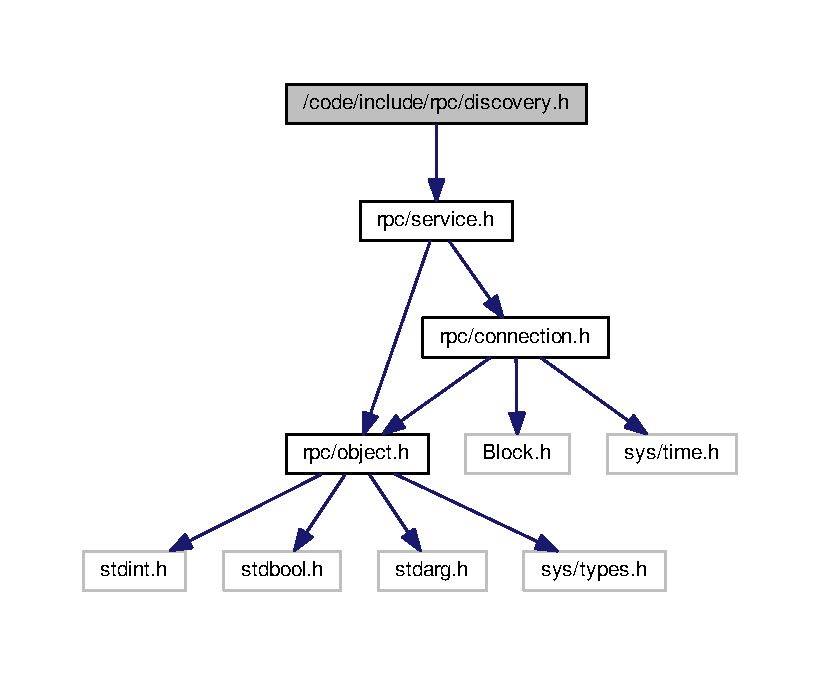
\includegraphics[width=350pt]{discovery_8h__incl}
\end{center}
\end{figure}
\subsection*{Functions}
\begin{DoxyCompactItemize}
\item 
int \hyperlink{discovery_8h_a282ce669d70603a2a80f99c3dc926d8f}{rpc\-\_\-discovery\-\_\-register} (rpc\-\_\-context\-\_\-t context)
\item 
int \hyperlink{discovery_8h_aef4a5ebeff7f32031a8ef8be116205bc}{rpc\-\_\-discovery\-\_\-destroy} (rpc\-\_\-context\-\_\-t context)
\end{DoxyCompactItemize}


\subsection{Detailed Description}
Helpers for creating auto-\/discoverable services. 

Definition in file \hyperlink{discovery_8h_source}{discovery.\-h}.



\subsection{Function Documentation}
\hypertarget{discovery_8h_aef4a5ebeff7f32031a8ef8be116205bc}{\index{discovery.\-h@{discovery.\-h}!rpc\-\_\-discovery\-\_\-destroy@{rpc\-\_\-discovery\-\_\-destroy}}
\index{rpc\-\_\-discovery\-\_\-destroy@{rpc\-\_\-discovery\-\_\-destroy}!discovery.h@{discovery.\-h}}
\subsubsection[{rpc\-\_\-discovery\-\_\-destroy}]{\setlength{\rightskip}{0pt plus 5cm}int rpc\-\_\-discovery\-\_\-destroy (
\begin{DoxyParamCaption}
\item[{rpc\-\_\-context\-\_\-t}]{context}
\end{DoxyParamCaption}
)}}\label{discovery_8h_aef4a5ebeff7f32031a8ef8be116205bc}
Uninstalls previously installed discovery service.


\begin{DoxyParams}{Parameters}
{\em context} & R\-P\-C context to uninstall discovery service from \\
\hline
\end{DoxyParams}
\begin{DoxyReturn}{Returns}
0 on success, -\/1 on failure 
\end{DoxyReturn}
\hypertarget{discovery_8h_a282ce669d70603a2a80f99c3dc926d8f}{\index{discovery.\-h@{discovery.\-h}!rpc\-\_\-discovery\-\_\-register@{rpc\-\_\-discovery\-\_\-register}}
\index{rpc\-\_\-discovery\-\_\-register@{rpc\-\_\-discovery\-\_\-register}!discovery.h@{discovery.\-h}}
\subsubsection[{rpc\-\_\-discovery\-\_\-register}]{\setlength{\rightskip}{0pt plus 5cm}int rpc\-\_\-discovery\-\_\-register (
\begin{DoxyParamCaption}
\item[{rpc\-\_\-context\-\_\-t}]{context}
\end{DoxyParamCaption}
)}}\label{discovery_8h_a282ce669d70603a2a80f99c3dc926d8f}
Installs discovery service on an R\-P\-C context.


\begin{DoxyParams}{Parameters}
{\em context} & R\-P\-C context to install on \\
\hline
\end{DoxyParams}
\begin{DoxyReturn}{Returns}
0 on success, -\/1 on failure 
\end{DoxyReturn}

\hypertarget{object_8h}{}\section{/code/include/rpc/object.h File Reference}
\label{object_8h}\index{/code/include/rpc/object.\+h@{/code/include/rpc/object.\+h}}
{\ttfamily \#include $<$stdint.\+h$>$}\newline
{\ttfamily \#include $<$stdbool.\+h$>$}\newline
{\ttfamily \#include $<$stdarg.\+h$>$}\newline
{\ttfamily \#include $<$sys/uio.\+h$>$}\newline
{\ttfamily \#include $<$sys/types.\+h$>$}\newline
Include dependency graph for object.\+h\+:
\nopagebreak
\begin{figure}[H]
\begin{center}
\leavevmode
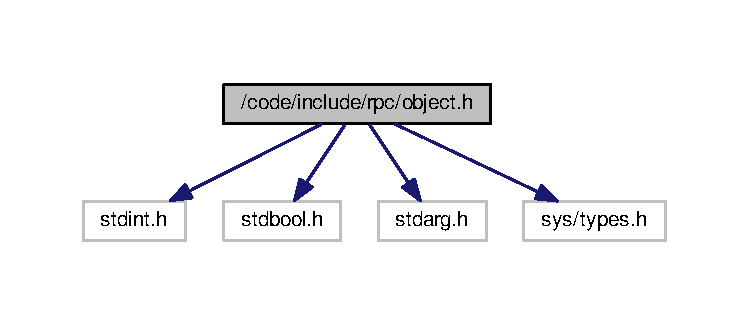
\includegraphics[width=350pt]{object_8h__incl}
\end{center}
\end{figure}
This graph shows which files directly or indirectly include this file\+:
\nopagebreak
\begin{figure}[H]
\begin{center}
\leavevmode
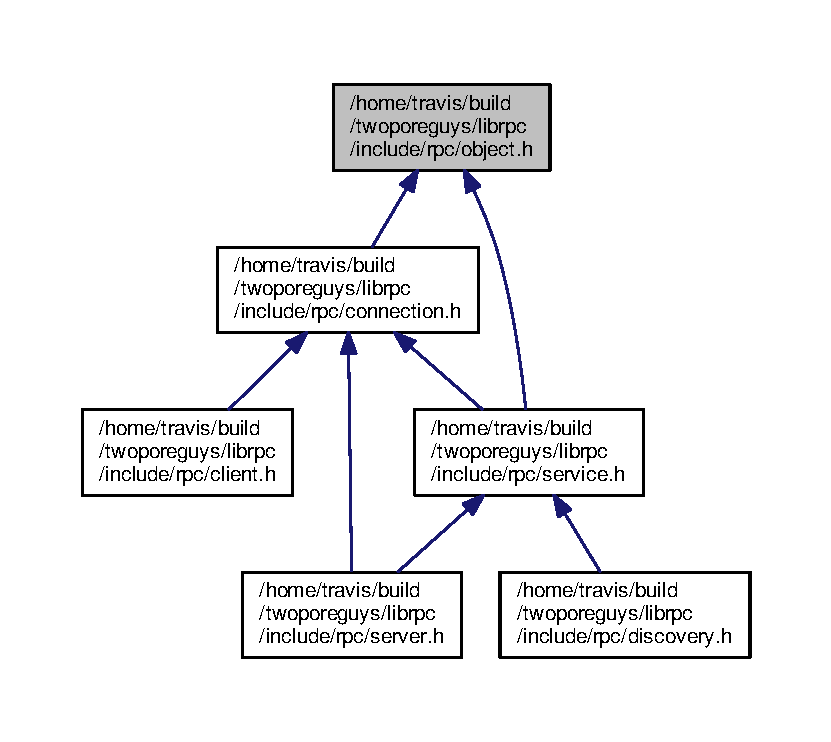
\includegraphics[width=350pt]{object_8h__dep__incl}
\end{center}
\end{figure}
\subsection*{Macros}
\begin{DoxyCompactItemize}
\item 
\#define \hyperlink{object_8h_a33c2b5ad21d20059d031e6a390021822}{R\+P\+C\+\_\+\+A\+R\+R\+A\+Y\+\_\+\+A\+P\+P\+L\+I\+ER}(\+\_\+fn,  \+\_\+arg)
\item 
\#define \hyperlink{object_8h_a814f85a172b4dae9c201063cad92514e}{R\+P\+C\+\_\+\+D\+I\+C\+T\+I\+O\+N\+A\+R\+Y\+\_\+\+A\+P\+P\+L\+I\+ER}(\+\_\+fn,  \+\_\+arg)
\item 
\#define \hyperlink{object_8h_af7b40854202a0a6708b0611b4fdf9121}{R\+P\+C\+\_\+\+A\+R\+R\+A\+Y\+\_\+\+C\+MP}(\+\_\+fn,  \+\_\+arg)
\item 
\#define \hyperlink{object_8h_a470d0e93b159810ff425aec90f47c817}{R\+P\+C\+\_\+\+B\+I\+N\+A\+R\+Y\+\_\+\+D\+E\+S\+T\+R\+U\+C\+T\+OR}(\+\_\+fn)
\item 
\#define \hyperlink{object_8h_a5b9fa1b598d399f5eacdbf2a8f86fd41}{R\+P\+C\+\_\+\+B\+I\+N\+A\+R\+Y\+\_\+\+D\+E\+S\+T\+R\+U\+C\+T\+O\+R\+\_\+\+A\+RG}(\+\_\+fn,  \+\_\+arg)
\item 
\#define \hyperlink{object_8h_aa125ec0a73c4c9953b07e5da1712573e}{rpc\+\_\+is\+\_\+error}(\+\_\+object)~(\hyperlink{object_8h_aa1f69b6cfaa4ae287272d76da16b005d}{rpc\+\_\+get\+\_\+type}(\+\_\+object) == \hyperlink{object_8h_a40ea3143863f0a2b47446ccaf655638ea7c63246a7c7bc5912d499fb117358506}{R\+P\+C\+\_\+\+T\+Y\+P\+E\+\_\+\+E\+R\+R\+OR})
\item 
\#define \hyperlink{object_8h_aac19be935f72b35eeb2851bc509eabb2}{rpc\+\_\+release}(\+\_\+object)
\item 
\#define \hyperlink{object_8h_a541e997e04e48fe86df08ae323516490}{rpc\+\_\+swap}(\+\_\+old,  \+\_\+new)
\item 
\#define \hyperlink{object_8h_aa2468583d15995a2451e3f2072631086}{rpc\+\_\+auto\+\_\+object\+\_\+t}~\+\_\+\+\_\+attribute\+\_\+\+\_\+((cleanup(\+\_\+\+\_\+rpc\+\_\+raii\+\_\+release))) \hyperlink{object_8h_ab365f726b4975c0c8376b808d111d01b}{rpc\+\_\+object\+\_\+t}
\end{DoxyCompactItemize}
\subsection*{Typedefs}
\begin{DoxyCompactItemize}
\item 
typedef struct rpc\+\_\+object $\ast$ \hyperlink{object_8h_ab365f726b4975c0c8376b808d111d01b}{rpc\+\_\+object\+\_\+t}
\item 
typedef bool($^\wedge$ \hyperlink{object_8h_a8a8f170096f2ea0286aecef9cabc79a7}{rpc\+\_\+array\+\_\+applier\+\_\+t}) (size\+\_\+t index, \+\_\+\+Nonnull \hyperlink{object_8h_ab365f726b4975c0c8376b808d111d01b}{rpc\+\_\+object\+\_\+t} value)
\item 
\mbox{\Hypertarget{object_8h_a93d201419f9a91a3126161a94fd1cb69}\label{object_8h_a93d201419f9a91a3126161a94fd1cb69}} 
typedef \+\_\+\+Nonnull \hyperlink{object_8h_ab365f726b4975c0c8376b808d111d01b}{rpc\+\_\+object\+\_\+t}($^\wedge$ {\bfseries rpc\+\_\+array\+\_\+mapper\+\_\+t}) (size\+\_\+t index, \+\_\+\+Nonnull \hyperlink{object_8h_ab365f726b4975c0c8376b808d111d01b}{rpc\+\_\+object\+\_\+t} value)
\item 
typedef bool($^\wedge$ \hyperlink{object_8h_a245b0bc0367303ab8083913323ae40ae}{rpc\+\_\+dictionary\+\_\+applier\+\_\+t}) (const char $\ast$\+\_\+\+Nonnull key, \+\_\+\+Nonnull \hyperlink{object_8h_ab365f726b4975c0c8376b808d111d01b}{rpc\+\_\+object\+\_\+t} value)
\item 
\mbox{\Hypertarget{object_8h_afdc48fdf7bc068a588f59d0d307e5041}\label{object_8h_afdc48fdf7bc068a588f59d0d307e5041}} 
typedef \+\_\+\+Nonnull \hyperlink{object_8h_ab365f726b4975c0c8376b808d111d01b}{rpc\+\_\+object\+\_\+t}($^\wedge$ {\bfseries rpc\+\_\+dictionary\+\_\+mapper\+\_\+t}) (const char $\ast$\+\_\+\+Nonnull key, \+\_\+\+Nonnull \hyperlink{object_8h_ab365f726b4975c0c8376b808d111d01b}{rpc\+\_\+object\+\_\+t} value)
\item 
typedef int($^\wedge$ \hyperlink{object_8h_a29f4de14614637dc5848764170dcd186}{rpc\+\_\+array\+\_\+cmp\+\_\+t}) (\+\_\+\+Nonnull \hyperlink{object_8h_ab365f726b4975c0c8376b808d111d01b}{rpc\+\_\+object\+\_\+t} o1, \+\_\+\+Nonnull \hyperlink{object_8h_ab365f726b4975c0c8376b808d111d01b}{rpc\+\_\+object\+\_\+t} o2)
\item 
typedef void($^\wedge$ \hyperlink{object_8h_af9a3ce2bd5f1b2c442a37baceccc4790}{rpc\+\_\+binary\+\_\+destructor\+\_\+t}) (void $\ast$\+\_\+\+Nullable)
\end{DoxyCompactItemize}
\subsection*{Enumerations}
\begin{DoxyCompactItemize}
\item 
enum \hyperlink{object_8h_a40ea3143863f0a2b47446ccaf655638e}{rpc\+\_\+type\+\_\+t} \{ \newline
\hyperlink{object_8h_a40ea3143863f0a2b47446ccaf655638ea71dacfbd072b09e8cbb22055447b660d}{R\+P\+C\+\_\+\+T\+Y\+P\+E\+\_\+\+N\+U\+LL}, 
\hyperlink{object_8h_a40ea3143863f0a2b47446ccaf655638ea318fdf911250c3ae135bb51839ff033d}{R\+P\+C\+\_\+\+T\+Y\+P\+E\+\_\+\+B\+O\+OL}, 
\hyperlink{object_8h_a40ea3143863f0a2b47446ccaf655638ea12702811680ffcd89bee08bf546e37f6}{R\+P\+C\+\_\+\+T\+Y\+P\+E\+\_\+\+U\+I\+N\+T64}, 
\hyperlink{object_8h_a40ea3143863f0a2b47446ccaf655638ea1f5294f7ab642ef8e693a2728d0ad31a}{R\+P\+C\+\_\+\+T\+Y\+P\+E\+\_\+\+I\+N\+T64}, 
\newline
\hyperlink{object_8h_a40ea3143863f0a2b47446ccaf655638ea81f15a333335dc830b45d39600491796}{R\+P\+C\+\_\+\+T\+Y\+P\+E\+\_\+\+D\+O\+U\+B\+LE}, 
\hyperlink{object_8h_a40ea3143863f0a2b47446ccaf655638ea8526a0ec0f1f9f9b06dac23b1c6aecb1}{R\+P\+C\+\_\+\+T\+Y\+P\+E\+\_\+\+D\+A\+TE}, 
\hyperlink{object_8h_a40ea3143863f0a2b47446ccaf655638ea8689ddb6d2be1e10f55b946fc89c7383}{R\+P\+C\+\_\+\+T\+Y\+P\+E\+\_\+\+S\+T\+R\+I\+NG}, 
\hyperlink{object_8h_a40ea3143863f0a2b47446ccaf655638ea25c2db26d03cddd947fd0b9486c66858}{R\+P\+C\+\_\+\+T\+Y\+P\+E\+\_\+\+B\+I\+N\+A\+RY}, 
\newline
\hyperlink{object_8h_a40ea3143863f0a2b47446ccaf655638ea7035c0eb69dd595be19d90a2e3c48ea9}{R\+P\+C\+\_\+\+T\+Y\+P\+E\+\_\+\+FD}, 
\hyperlink{object_8h_a40ea3143863f0a2b47446ccaf655638ea5dd9c67e5ca75573ddac3129e5430386}{R\+P\+C\+\_\+\+T\+Y\+P\+E\+\_\+\+D\+I\+C\+T\+I\+O\+N\+A\+RY}, 
\hyperlink{object_8h_a40ea3143863f0a2b47446ccaf655638eab4f0a2ba87efaf952a1008c0771d7f5a}{R\+P\+C\+\_\+\+T\+Y\+P\+E\+\_\+\+A\+R\+R\+AY}, 
\hyperlink{object_8h_a40ea3143863f0a2b47446ccaf655638ea7c63246a7c7bc5912d499fb117358506}{R\+P\+C\+\_\+\+T\+Y\+P\+E\+\_\+\+E\+R\+R\+OR}
 \}
\end{DoxyCompactItemize}
\subsection*{Functions}
\begin{DoxyCompactItemize}
\item 
\+\_\+\+Nonnull \hyperlink{object_8h_ab365f726b4975c0c8376b808d111d01b}{rpc\+\_\+object\+\_\+t} \hyperlink{object_8h_a38666db12609d1a1f5c856a7f3f0a03a}{rpc\+\_\+retain} (\+\_\+\+Nonnull \hyperlink{object_8h_ab365f726b4975c0c8376b808d111d01b}{rpc\+\_\+object\+\_\+t} object)
\item 
int \hyperlink{object_8h_aef96805793fdeeb98b88d03890d034ba}{rpc\+\_\+release\+\_\+impl} (\+\_\+\+Nonnull \hyperlink{object_8h_ab365f726b4975c0c8376b808d111d01b}{rpc\+\_\+object\+\_\+t} object)
\item 
int \hyperlink{object_8h_a304648476e1f6a68cd9c2521a7703824}{rpc\+\_\+get\+\_\+refcount} (\+\_\+\+Nullable \hyperlink{object_8h_ab365f726b4975c0c8376b808d111d01b}{rpc\+\_\+object\+\_\+t} object)
\item 
int \hyperlink{object_8h_a9ec7986f5515c359eb4ce86b7d9afa64}{rpc\+\_\+get\+\_\+count} (bool all)
\item 
size\+\_\+t \hyperlink{object_8h_a7cfb70b97eaa92aec1888ff177b3100d}{rpc\+\_\+get\+\_\+line\+\_\+number} (\+\_\+\+Nonnull \hyperlink{object_8h_ab365f726b4975c0c8376b808d111d01b}{rpc\+\_\+object\+\_\+t} object)
\item 
size\+\_\+t \hyperlink{object_8h_ac2b74c41ca419b2daca6ffb7123a1fb7}{rpc\+\_\+get\+\_\+column\+\_\+number} (\+\_\+\+Nonnull \hyperlink{object_8h_ab365f726b4975c0c8376b808d111d01b}{rpc\+\_\+object\+\_\+t} object)
\item 
\+\_\+\+Nonnull \hyperlink{object_8h_ab365f726b4975c0c8376b808d111d01b}{rpc\+\_\+object\+\_\+t} \hyperlink{object_8h_a14ffadb854f6dfe280235c819ba92030}{rpc\+\_\+copy} (\+\_\+\+Nonnull \hyperlink{object_8h_ab365f726b4975c0c8376b808d111d01b}{rpc\+\_\+object\+\_\+t} object)
\item 
int \hyperlink{object_8h_aecda48bd48de2015e2c698c5903d5b9e}{rpc\+\_\+cmp} (\+\_\+\+Nullable \hyperlink{object_8h_ab365f726b4975c0c8376b808d111d01b}{rpc\+\_\+object\+\_\+t} o1, \+\_\+\+Nullable \hyperlink{object_8h_ab365f726b4975c0c8376b808d111d01b}{rpc\+\_\+object\+\_\+t} o2)
\item 
bool \hyperlink{object_8h_a549898ba27326cf9141c97f20cab20d5}{rpc\+\_\+equal} (\+\_\+\+Nullable \hyperlink{object_8h_ab365f726b4975c0c8376b808d111d01b}{rpc\+\_\+object\+\_\+t} o1, \+\_\+\+Nullable \hyperlink{object_8h_ab365f726b4975c0c8376b808d111d01b}{rpc\+\_\+object\+\_\+t} o2)
\item 
size\+\_\+t \hyperlink{object_8h_a3720cffe268a0d3b90a8d7b292325c5c}{rpc\+\_\+hash} (\+\_\+\+Nonnull \hyperlink{object_8h_ab365f726b4975c0c8376b808d111d01b}{rpc\+\_\+object\+\_\+t} object)
\item 
char $\ast$\+\_\+\+Nonnull \hyperlink{object_8h_ac3266a5b20add52514c1b2c70a4a5878}{rpc\+\_\+copy\+\_\+description} (\+\_\+\+Nonnull \hyperlink{object_8h_ab365f726b4975c0c8376b808d111d01b}{rpc\+\_\+object\+\_\+t} object)
\item 
\hyperlink{object_8h_a40ea3143863f0a2b47446ccaf655638e}{rpc\+\_\+type\+\_\+t} \hyperlink{object_8h_aa1f69b6cfaa4ae287272d76da16b005d}{rpc\+\_\+get\+\_\+type} (\+\_\+\+Nonnull \hyperlink{object_8h_ab365f726b4975c0c8376b808d111d01b}{rpc\+\_\+object\+\_\+t} object)
\item 
const char $\ast$\+\_\+\+Nullable \hyperlink{object_8h_a9627e5627f82660af36d6c626aebabbd}{rpc\+\_\+get\+\_\+type\+\_\+name} (\hyperlink{object_8h_a40ea3143863f0a2b47446ccaf655638e}{rpc\+\_\+type\+\_\+t} type)
\item 
\+\_\+\+Nullable \hyperlink{object_8h_ab365f726b4975c0c8376b808d111d01b}{rpc\+\_\+object\+\_\+t} \hyperlink{object_8h_a45800949eb1b61b3af02051c780244fe}{rpc\+\_\+get\+\_\+last\+\_\+error} (void)
\item 
\+\_\+\+Nullable \hyperlink{object_8h_ab365f726b4975c0c8376b808d111d01b}{rpc\+\_\+object\+\_\+t} \hyperlink{object_8h_a8a8454f12dcde323f5daba961febea97}{rpc\+\_\+object\+\_\+pack} (const char $\ast$\+\_\+\+Nonnull fmt,...)
\item 
\+\_\+\+Nullable \hyperlink{object_8h_ab365f726b4975c0c8376b808d111d01b}{rpc\+\_\+object\+\_\+t} \hyperlink{object_8h_a3c15ce52778038cf6bbfe191cf30fe71}{rpc\+\_\+object\+\_\+vpack} (const char $\ast$\+\_\+\+Nonnull fmt, va\+\_\+list ap)
\item 
int \hyperlink{object_8h_a6ff01b9e6d71ba03e2dff76ede7366f6}{rpc\+\_\+object\+\_\+unpack} (\+\_\+\+Nonnull \hyperlink{object_8h_ab365f726b4975c0c8376b808d111d01b}{rpc\+\_\+object\+\_\+t}, const char $\ast$\+\_\+\+Nonnull fmt,...)
\item 
int \hyperlink{object_8h_aacdca2e75cc35de88ff0282c17dda05d}{rpc\+\_\+object\+\_\+vunpack} (\+\_\+\+Nonnull \hyperlink{object_8h_ab365f726b4975c0c8376b808d111d01b}{rpc\+\_\+object\+\_\+t}, const char $\ast$\+\_\+\+Nonnull fmt, va\+\_\+list ap)
\item 
\+\_\+\+Nonnull \hyperlink{object_8h_ab365f726b4975c0c8376b808d111d01b}{rpc\+\_\+object\+\_\+t} \hyperlink{object_8h_af71ab5e00bfb82e6733e59c42e3ed157}{rpc\+\_\+null\+\_\+create} (void)
\item 
\+\_\+\+Nonnull \hyperlink{object_8h_ab365f726b4975c0c8376b808d111d01b}{rpc\+\_\+object\+\_\+t} \hyperlink{object_8h_af1b839aeabfc9be778224c3d191cafdc}{rpc\+\_\+bool\+\_\+create} (bool value)
\item 
bool \hyperlink{object_8h_ac2298d4c51a389269922f24ac4a398e2}{rpc\+\_\+bool\+\_\+get\+\_\+value} (\+\_\+\+Nonnull \hyperlink{object_8h_ab365f726b4975c0c8376b808d111d01b}{rpc\+\_\+object\+\_\+t} xbool)
\item 
\+\_\+\+Nonnull \hyperlink{object_8h_ab365f726b4975c0c8376b808d111d01b}{rpc\+\_\+object\+\_\+t} \hyperlink{object_8h_a8c515bb8b1add8dbe86e615f048182a2}{rpc\+\_\+int64\+\_\+create} (int64\+\_\+t value)
\item 
int64\+\_\+t \hyperlink{object_8h_a0be879b57e12261e08ca893eecefe408}{rpc\+\_\+int64\+\_\+get\+\_\+value} (\+\_\+\+Nonnull \hyperlink{object_8h_ab365f726b4975c0c8376b808d111d01b}{rpc\+\_\+object\+\_\+t} xint)
\item 
\+\_\+\+Nonnull \hyperlink{object_8h_ab365f726b4975c0c8376b808d111d01b}{rpc\+\_\+object\+\_\+t} \hyperlink{object_8h_ad7dd5248202a7efab7a64dfece626efe}{rpc\+\_\+uint64\+\_\+create} (uint64\+\_\+t value)
\item 
uint64\+\_\+t \hyperlink{object_8h_aeba41bff814c285e2160b105eb83c8aa}{rpc\+\_\+uint64\+\_\+get\+\_\+value} (\+\_\+\+Nonnull \hyperlink{object_8h_ab365f726b4975c0c8376b808d111d01b}{rpc\+\_\+object\+\_\+t} xuint)
\item 
\+\_\+\+Nonnull \hyperlink{object_8h_ab365f726b4975c0c8376b808d111d01b}{rpc\+\_\+object\+\_\+t} \hyperlink{object_8h_ac4969a4bcf0cac08d29ae0e55d201c4b}{rpc\+\_\+double\+\_\+create} (double value)
\item 
double \hyperlink{object_8h_a64d3e83ce3cfe82b583f2e471f9cd2c1}{rpc\+\_\+double\+\_\+get\+\_\+value} (\+\_\+\+Nonnull \hyperlink{object_8h_ab365f726b4975c0c8376b808d111d01b}{rpc\+\_\+object\+\_\+t} xdouble)
\item 
\+\_\+\+Nonnull \hyperlink{object_8h_ab365f726b4975c0c8376b808d111d01b}{rpc\+\_\+object\+\_\+t} \hyperlink{object_8h_ad82b3e29d3480a85002f057a1090f55a}{rpc\+\_\+date\+\_\+create} (int64\+\_\+t interval)
\item 
\+\_\+\+Nonnull \hyperlink{object_8h_ab365f726b4975c0c8376b808d111d01b}{rpc\+\_\+object\+\_\+t} \hyperlink{object_8h_a4dea860dff672ec333ff08de73867ec9}{rpc\+\_\+date\+\_\+create\+\_\+from\+\_\+current} (void)
\item 
int64\+\_\+t \hyperlink{object_8h_aaa0b31994b3093e3e183ef9f0f1e6940}{rpc\+\_\+date\+\_\+get\+\_\+value} (\+\_\+\+Nonnull \hyperlink{object_8h_ab365f726b4975c0c8376b808d111d01b}{rpc\+\_\+object\+\_\+t} xdate)
\item 
\+\_\+\+Nonnull \hyperlink{object_8h_ab365f726b4975c0c8376b808d111d01b}{rpc\+\_\+object\+\_\+t} \hyperlink{object_8h_acf509ab42ce47d0b4c0ce1951c0c11af}{rpc\+\_\+data\+\_\+create} (const void $\ast$\+\_\+\+Nullable bytes, size\+\_\+t length, \+\_\+\+Nullable \hyperlink{object_8h_af9a3ce2bd5f1b2c442a37baceccc4790}{rpc\+\_\+binary\+\_\+destructor\+\_\+t} destructor)
\item 
\+\_\+\+Nonnull \hyperlink{object_8h_ab365f726b4975c0c8376b808d111d01b}{rpc\+\_\+object\+\_\+t} \hyperlink{object_8h_a81716cdca66934bee041b7fdefad94e7}{rpc\+\_\+data\+\_\+create\+\_\+iov} (struct iovec $\ast$\+\_\+\+Nonnull iov, size\+\_\+t niov)
\item 
size\+\_\+t \hyperlink{object_8h_a668d3befabd7ae069e381f0cf7ab6f15}{rpc\+\_\+data\+\_\+get\+\_\+length} (\+\_\+\+Nonnull \hyperlink{object_8h_ab365f726b4975c0c8376b808d111d01b}{rpc\+\_\+object\+\_\+t} xdata)
\item 
const void $\ast$\+\_\+\+Nullable \hyperlink{object_8h_a73259e1914dbb4c18a995768a7d3930b}{rpc\+\_\+data\+\_\+get\+\_\+bytes\+\_\+ptr} (\+\_\+\+Nonnull \hyperlink{object_8h_ab365f726b4975c0c8376b808d111d01b}{rpc\+\_\+object\+\_\+t} xdata)
\item 
size\+\_\+t \hyperlink{object_8h_ab5d1feb11fc902658b7fe53bf7cc1627}{rpc\+\_\+data\+\_\+get\+\_\+bytes} (\+\_\+\+Nonnull \hyperlink{object_8h_ab365f726b4975c0c8376b808d111d01b}{rpc\+\_\+object\+\_\+t} xdata, void $\ast$\+\_\+\+Nonnull buffer, size\+\_\+t off, size\+\_\+t length)
\item 
\+\_\+\+Nonnull \hyperlink{object_8h_ab365f726b4975c0c8376b808d111d01b}{rpc\+\_\+object\+\_\+t} \hyperlink{object_8h_ae7ba5d4d5a269764aaac74170be2884c}{rpc\+\_\+string\+\_\+create} (const char $\ast$\+\_\+\+Nonnull string)
\item 
\+\_\+\+Nonnull \hyperlink{object_8h_ab365f726b4975c0c8376b808d111d01b}{rpc\+\_\+object\+\_\+t} \hyperlink{object_8h_a227a4ec7bd24bd07dd68678d4900340e}{rpc\+\_\+string\+\_\+create\+\_\+len} (const char $\ast$\+\_\+\+Nonnull string, size\+\_\+t length)
\item 
\+\_\+\+Nonnull \hyperlink{object_8h_ab365f726b4975c0c8376b808d111d01b}{rpc\+\_\+object\+\_\+t} \hyperlink{object_8h_a90b42194b061a3f7c010cfbd67e43e06}{rpc\+\_\+string\+\_\+create\+\_\+with\+\_\+format} (const char $\ast$\+\_\+\+Nonnull fmt,...)
\item 
\+\_\+\+Nonnull \hyperlink{object_8h_ab365f726b4975c0c8376b808d111d01b}{rpc\+\_\+object\+\_\+t} \hyperlink{object_8h_a2ee591e97432340d93de769e723c6f92}{rpc\+\_\+string\+\_\+create\+\_\+with\+\_\+format\+\_\+and\+\_\+arguments} (const char $\ast$\+\_\+\+Nonnull fmt, va\+\_\+list ap)
\item 
size\+\_\+t \hyperlink{object_8h_a1fe4187920e3b5b436f1b76773e5cc3c}{rpc\+\_\+string\+\_\+get\+\_\+length} (\+\_\+\+Nonnull \hyperlink{object_8h_ab365f726b4975c0c8376b808d111d01b}{rpc\+\_\+object\+\_\+t} xstring)
\item 
const char $\ast$\+\_\+\+Nullable \hyperlink{object_8h_a04a698c1f5f736ef71bc81ccf91be52d}{rpc\+\_\+string\+\_\+get\+\_\+string\+\_\+ptr} (\+\_\+\+Nonnull \hyperlink{object_8h_ab365f726b4975c0c8376b808d111d01b}{rpc\+\_\+object\+\_\+t} xstring)
\item 
\+\_\+\+Nonnull \hyperlink{object_8h_ab365f726b4975c0c8376b808d111d01b}{rpc\+\_\+object\+\_\+t} \hyperlink{object_8h_aa2e6228045667b4e13b9897cfd2dc072}{rpc\+\_\+fd\+\_\+create} (int fd)
\item 
int \hyperlink{object_8h_a1c9845210494039bf2e3c27027efaa55}{rpc\+\_\+fd\+\_\+dup} (\+\_\+\+Nonnull \hyperlink{object_8h_ab365f726b4975c0c8376b808d111d01b}{rpc\+\_\+object\+\_\+t} xfd)
\item 
int \hyperlink{object_8h_a2aafc3a2617aee1a4437d417ba33b807}{rpc\+\_\+fd\+\_\+get\+\_\+value} (\+\_\+\+Nonnull \hyperlink{object_8h_ab365f726b4975c0c8376b808d111d01b}{rpc\+\_\+object\+\_\+t} xfd)
\item 
\+\_\+\+Nonnull \hyperlink{object_8h_ab365f726b4975c0c8376b808d111d01b}{rpc\+\_\+object\+\_\+t} \hyperlink{object_8h_ae543b86020ed2e2e8fd483c38e31552a}{rpc\+\_\+array\+\_\+create} (void)
\item 
\+\_\+\+Nonnull \hyperlink{object_8h_ab365f726b4975c0c8376b808d111d01b}{rpc\+\_\+object\+\_\+t} \hyperlink{object_8h_aa295b053a235f3c3a03470da644b36f5}{rpc\+\_\+array\+\_\+create\+\_\+ex} (const \+\_\+\+Nonnull \hyperlink{object_8h_ab365f726b4975c0c8376b808d111d01b}{rpc\+\_\+object\+\_\+t} $\ast$\+\_\+\+Nonnull objects, size\+\_\+t count, bool steal)
\item 
void \hyperlink{object_8h_af53ea18b86140d9570a7133ac9beda82}{rpc\+\_\+array\+\_\+set\+\_\+value} (\+\_\+\+Nonnull \hyperlink{object_8h_ab365f726b4975c0c8376b808d111d01b}{rpc\+\_\+object\+\_\+t} array, size\+\_\+t index, \+\_\+\+Nullable \hyperlink{object_8h_ab365f726b4975c0c8376b808d111d01b}{rpc\+\_\+object\+\_\+t} value)
\item 
void \hyperlink{object_8h_a6cce558875dd3007c4939ddf48d8eeb5}{rpc\+\_\+array\+\_\+steal\+\_\+value} (\+\_\+\+Nonnull \hyperlink{object_8h_ab365f726b4975c0c8376b808d111d01b}{rpc\+\_\+object\+\_\+t} array, size\+\_\+t index, \+\_\+\+Nullable \hyperlink{object_8h_ab365f726b4975c0c8376b808d111d01b}{rpc\+\_\+object\+\_\+t} value)
\item 
void \hyperlink{object_8h_a849e9e86878d651edbcbb861fdb6a44b}{rpc\+\_\+array\+\_\+remove\+\_\+index} (\+\_\+\+Nonnull \hyperlink{object_8h_ab365f726b4975c0c8376b808d111d01b}{rpc\+\_\+object\+\_\+t} array, size\+\_\+t index)
\item 
void \hyperlink{object_8h_a325a04c3c3f91ebbece34b5e816e1032}{rpc\+\_\+array\+\_\+remove\+\_\+all} (\+\_\+\+Nonnull \hyperlink{object_8h_ab365f726b4975c0c8376b808d111d01b}{rpc\+\_\+object\+\_\+t} array)
\item 
void \hyperlink{object_8h_ad7facdb473b73004ea3829ba6bf48b83}{rpc\+\_\+array\+\_\+append\+\_\+value} (\+\_\+\+Nonnull \hyperlink{object_8h_ab365f726b4975c0c8376b808d111d01b}{rpc\+\_\+object\+\_\+t} array, \+\_\+\+Nonnull \hyperlink{object_8h_ab365f726b4975c0c8376b808d111d01b}{rpc\+\_\+object\+\_\+t} value)
\item 
void \hyperlink{object_8h_ad880c9b3591ff9be8ed8127afe3af72c}{rpc\+\_\+array\+\_\+append\+\_\+stolen\+\_\+value} (\+\_\+\+Nonnull \hyperlink{object_8h_ab365f726b4975c0c8376b808d111d01b}{rpc\+\_\+object\+\_\+t} array, \+\_\+\+Nonnull \hyperlink{object_8h_ab365f726b4975c0c8376b808d111d01b}{rpc\+\_\+object\+\_\+t} value)
\item 
\+\_\+\+Nullable \hyperlink{object_8h_ab365f726b4975c0c8376b808d111d01b}{rpc\+\_\+object\+\_\+t} \hyperlink{object_8h_acb9f788d4b87668b12c0b2b7ea561ec4}{rpc\+\_\+array\+\_\+get\+\_\+value} (\+\_\+\+Nonnull \hyperlink{object_8h_ab365f726b4975c0c8376b808d111d01b}{rpc\+\_\+object\+\_\+t} array, size\+\_\+t index)
\item 
size\+\_\+t \hyperlink{object_8h_a1c0ce68df7e7805bc19cf2eb219b0c96}{rpc\+\_\+array\+\_\+get\+\_\+count} (\+\_\+\+Nonnull \hyperlink{object_8h_ab365f726b4975c0c8376b808d111d01b}{rpc\+\_\+object\+\_\+t} array)
\item 
bool \hyperlink{object_8h_ac2329e9bc24d6d55b1b9ee030cea4e33}{rpc\+\_\+array\+\_\+apply} (\+\_\+\+Nonnull \hyperlink{object_8h_ab365f726b4975c0c8376b808d111d01b}{rpc\+\_\+object\+\_\+t} array, \+\_\+\+Nonnull \hyperlink{object_8h_a8a8f170096f2ea0286aecef9cabc79a7}{rpc\+\_\+array\+\_\+applier\+\_\+t} applier)
\item 
void \hyperlink{object_8h_af435318648f57712e627636a37f39372}{rpc\+\_\+array\+\_\+map} (\+\_\+\+Nonnull \hyperlink{object_8h_ab365f726b4975c0c8376b808d111d01b}{rpc\+\_\+object\+\_\+t} array, \+\_\+\+Nonnull rpc\+\_\+array\+\_\+mapper\+\_\+t mapper)
\item 
bool \hyperlink{object_8h_a5ea27ad4516e4192959de93db8bb45fa}{rpc\+\_\+array\+\_\+contains} (\+\_\+\+Nonnull \hyperlink{object_8h_ab365f726b4975c0c8376b808d111d01b}{rpc\+\_\+object\+\_\+t} array, \+\_\+\+Nonnull \hyperlink{object_8h_ab365f726b4975c0c8376b808d111d01b}{rpc\+\_\+object\+\_\+t} value)
\item 
bool \hyperlink{object_8h_ad83e5f334c3a9cfc983052be3e1fd2f9}{rpc\+\_\+array\+\_\+reverse\+\_\+apply} (\+\_\+\+Nonnull \hyperlink{object_8h_ab365f726b4975c0c8376b808d111d01b}{rpc\+\_\+object\+\_\+t} array, \+\_\+\+Nonnull \hyperlink{object_8h_a8a8f170096f2ea0286aecef9cabc79a7}{rpc\+\_\+array\+\_\+applier\+\_\+t} applier)
\item 
void \hyperlink{object_8h_a51ae0094f462c3af8823cdcba9131a5c}{rpc\+\_\+array\+\_\+sort} (\+\_\+\+Nonnull \hyperlink{object_8h_ab365f726b4975c0c8376b808d111d01b}{rpc\+\_\+object\+\_\+t} array, \+\_\+\+Nonnull \hyperlink{object_8h_a29f4de14614637dc5848764170dcd186}{rpc\+\_\+array\+\_\+cmp\+\_\+t} comparator)
\item 
\+\_\+\+Nonnull \hyperlink{object_8h_ab365f726b4975c0c8376b808d111d01b}{rpc\+\_\+object\+\_\+t} \hyperlink{object_8h_a6380e4e29867c57b5d5a69453a1221a4}{rpc\+\_\+array\+\_\+slice} (\+\_\+\+Nonnull \hyperlink{object_8h_ab365f726b4975c0c8376b808d111d01b}{rpc\+\_\+object\+\_\+t} array, size\+\_\+t start, ssize\+\_\+t len)
\item 
void \hyperlink{object_8h_ae64c6fed59094098027ded1ef538d375}{rpc\+\_\+array\+\_\+set\+\_\+bool} (\+\_\+\+Nonnull \hyperlink{object_8h_ab365f726b4975c0c8376b808d111d01b}{rpc\+\_\+object\+\_\+t} array, size\+\_\+t index, bool value)
\item 
void \hyperlink{object_8h_a2ae7c934dfe460fb860a196c572a22fb}{rpc\+\_\+array\+\_\+set\+\_\+int64} (\+\_\+\+Nonnull \hyperlink{object_8h_ab365f726b4975c0c8376b808d111d01b}{rpc\+\_\+object\+\_\+t} array, size\+\_\+t index, int64\+\_\+t value)
\item 
void \hyperlink{object_8h_a0d1299bb26d314bc66ae5881854e2bc6}{rpc\+\_\+array\+\_\+set\+\_\+uint64} (\+\_\+\+Nonnull \hyperlink{object_8h_ab365f726b4975c0c8376b808d111d01b}{rpc\+\_\+object\+\_\+t} array, size\+\_\+t index, uint64\+\_\+t value)
\item 
void \hyperlink{object_8h_a332af319e18eff8af830ccb4b5403351}{rpc\+\_\+array\+\_\+set\+\_\+double} (\+\_\+\+Nonnull \hyperlink{object_8h_ab365f726b4975c0c8376b808d111d01b}{rpc\+\_\+object\+\_\+t} array, size\+\_\+t index, double value)
\item 
void \hyperlink{object_8h_ad66c086eb95c68c552eb97253a1133c2}{rpc\+\_\+array\+\_\+set\+\_\+date} (\+\_\+\+Nonnull \hyperlink{object_8h_ab365f726b4975c0c8376b808d111d01b}{rpc\+\_\+object\+\_\+t} array, size\+\_\+t index, int64\+\_\+t value)
\item 
void \hyperlink{object_8h_a6b45dfb1fec47c8f3e7ea1bc0aa079f8}{rpc\+\_\+array\+\_\+set\+\_\+data} (\+\_\+\+Nonnull \hyperlink{object_8h_ab365f726b4975c0c8376b808d111d01b}{rpc\+\_\+object\+\_\+t} array, size\+\_\+t index, const void $\ast$\+\_\+\+Nullable bytes, size\+\_\+t length)
\item 
void \hyperlink{object_8h_a5c3515b51666d170e3984fc455041212}{rpc\+\_\+array\+\_\+set\+\_\+string} (\+\_\+\+Nonnull \hyperlink{object_8h_ab365f726b4975c0c8376b808d111d01b}{rpc\+\_\+object\+\_\+t} array, size\+\_\+t index, const char $\ast$\+\_\+\+Nonnull value)
\item 
void \hyperlink{object_8h_aa02fab0439778874d23d04a8b28b5145}{rpc\+\_\+array\+\_\+set\+\_\+fd} (\+\_\+\+Nonnull \hyperlink{object_8h_ab365f726b4975c0c8376b808d111d01b}{rpc\+\_\+object\+\_\+t} array, size\+\_\+t index, int value)
\item 
bool \hyperlink{object_8h_a201b7b860b53d529a32ae39b9d36e9af}{rpc\+\_\+array\+\_\+get\+\_\+bool} (\+\_\+\+Nonnull \hyperlink{object_8h_ab365f726b4975c0c8376b808d111d01b}{rpc\+\_\+object\+\_\+t} array, size\+\_\+t index)
\item 
int64\+\_\+t \hyperlink{object_8h_acad326352e89266883cf0f387cc60b23}{rpc\+\_\+array\+\_\+get\+\_\+int64} (\+\_\+\+Nonnull \hyperlink{object_8h_ab365f726b4975c0c8376b808d111d01b}{rpc\+\_\+object\+\_\+t} array, size\+\_\+t index)
\item 
uint64\+\_\+t \hyperlink{object_8h_a160f2347882c19b5d7c2e9c2b9d38ed7}{rpc\+\_\+array\+\_\+get\+\_\+uint64} (\+\_\+\+Nonnull \hyperlink{object_8h_ab365f726b4975c0c8376b808d111d01b}{rpc\+\_\+object\+\_\+t} array, size\+\_\+t index)
\item 
double \hyperlink{object_8h_aa8c1e3b70cdb55ff329b18769a1d42ae}{rpc\+\_\+array\+\_\+get\+\_\+double} (\+\_\+\+Nonnull \hyperlink{object_8h_ab365f726b4975c0c8376b808d111d01b}{rpc\+\_\+object\+\_\+t} array, size\+\_\+t index)
\item 
int64\+\_\+t \hyperlink{object_8h_ac8d5f4da00e7f5792a245259d14d9695}{rpc\+\_\+array\+\_\+get\+\_\+date} (\+\_\+\+Nonnull \hyperlink{object_8h_ab365f726b4975c0c8376b808d111d01b}{rpc\+\_\+object\+\_\+t} array, size\+\_\+t index)
\item 
const void $\ast$\+\_\+\+Nullable \hyperlink{object_8h_a0296e282242c13a4bc293d7c94e5b045}{rpc\+\_\+array\+\_\+get\+\_\+data} (\+\_\+\+Nonnull \hyperlink{object_8h_ab365f726b4975c0c8376b808d111d01b}{rpc\+\_\+object\+\_\+t} array, size\+\_\+t index, size\+\_\+t $\ast$\+\_\+\+Nullable length)
\item 
const char $\ast$\+\_\+\+Nullable \hyperlink{object_8h_a98483eea7ea6929d45d04b987a4c8f1c}{rpc\+\_\+array\+\_\+get\+\_\+string} (\+\_\+\+Nonnull \hyperlink{object_8h_ab365f726b4975c0c8376b808d111d01b}{rpc\+\_\+object\+\_\+t} array, size\+\_\+t index)
\item 
int \hyperlink{object_8h_aeac7c0ce4dad298b73204485fd87c9bf}{rpc\+\_\+array\+\_\+get\+\_\+fd} (\+\_\+\+Nonnull \hyperlink{object_8h_ab365f726b4975c0c8376b808d111d01b}{rpc\+\_\+object\+\_\+t} array, size\+\_\+t index)
\item 
int \hyperlink{object_8h_ace1549f30196cfeb56df7c3f8defdde3}{rpc\+\_\+array\+\_\+dup\+\_\+fd} (\+\_\+\+Nonnull \hyperlink{object_8h_ab365f726b4975c0c8376b808d111d01b}{rpc\+\_\+object\+\_\+t} array, size\+\_\+t index)
\item 
\+\_\+\+Nonnull \hyperlink{object_8h_ab365f726b4975c0c8376b808d111d01b}{rpc\+\_\+object\+\_\+t} \hyperlink{object_8h_a73972595ec8446bff84ef2b039ca9c25}{rpc\+\_\+error\+\_\+create} (int code, const char $\ast$\+\_\+\+Nonnull msg, \+\_\+\+Nullable \hyperlink{object_8h_ab365f726b4975c0c8376b808d111d01b}{rpc\+\_\+object\+\_\+t} extra)
\item 
\+\_\+\+Nonnull \hyperlink{object_8h_ab365f726b4975c0c8376b808d111d01b}{rpc\+\_\+object\+\_\+t} \hyperlink{object_8h_a158d631a26ec3aad80f745b6164f2281}{rpc\+\_\+error\+\_\+create\+\_\+with\+\_\+stack} (int code, const char $\ast$\+\_\+\+Nonnull msg, \+\_\+\+Nullable \hyperlink{object_8h_ab365f726b4975c0c8376b808d111d01b}{rpc\+\_\+object\+\_\+t} extra, \+\_\+\+Nullable \hyperlink{object_8h_ab365f726b4975c0c8376b808d111d01b}{rpc\+\_\+object\+\_\+t} stack)
\item 
int \hyperlink{object_8h_a0dd0c2fb523cd36216a93bbacb68f934}{rpc\+\_\+error\+\_\+get\+\_\+code} (\+\_\+\+Nonnull \hyperlink{object_8h_ab365f726b4975c0c8376b808d111d01b}{rpc\+\_\+object\+\_\+t} error)
\item 
const char $\ast$\+\_\+\+Nullable \hyperlink{object_8h_ac35bbbc0527c6590bdf50e55e7f08b6e}{rpc\+\_\+error\+\_\+get\+\_\+message} (\+\_\+\+Nonnull \hyperlink{object_8h_ab365f726b4975c0c8376b808d111d01b}{rpc\+\_\+object\+\_\+t} error)
\item 
\+\_\+\+Nullable \hyperlink{object_8h_ab365f726b4975c0c8376b808d111d01b}{rpc\+\_\+object\+\_\+t} \hyperlink{object_8h_a57e48ece0a70e0e8847e5c6d6c2effe7}{rpc\+\_\+error\+\_\+get\+\_\+extra} (\+\_\+\+Nonnull \hyperlink{object_8h_ab365f726b4975c0c8376b808d111d01b}{rpc\+\_\+object\+\_\+t} error)
\item 
void \hyperlink{object_8h_adb9bda2bdfc31587cebe0814b00e757e}{rpc\+\_\+error\+\_\+set\+\_\+extra} (\+\_\+\+Nonnull \hyperlink{object_8h_ab365f726b4975c0c8376b808d111d01b}{rpc\+\_\+object\+\_\+t} error, \+\_\+\+Nonnull \hyperlink{object_8h_ab365f726b4975c0c8376b808d111d01b}{rpc\+\_\+object\+\_\+t} extra)
\item 
\+\_\+\+Nullable \hyperlink{object_8h_ab365f726b4975c0c8376b808d111d01b}{rpc\+\_\+object\+\_\+t} \hyperlink{object_8h_a039cff664d5a098865b7d14bd9fe8df7}{rpc\+\_\+error\+\_\+get\+\_\+stack} (\+\_\+\+Nonnull \hyperlink{object_8h_ab365f726b4975c0c8376b808d111d01b}{rpc\+\_\+object\+\_\+t} error)
\item 
\+\_\+\+Nonnull \hyperlink{object_8h_ab365f726b4975c0c8376b808d111d01b}{rpc\+\_\+object\+\_\+t} \hyperlink{object_8h_afab55864a729d5a19cb3036ff468046f}{rpc\+\_\+dictionary\+\_\+create} (void)
\item 
\+\_\+\+Nonnull \hyperlink{object_8h_ab365f726b4975c0c8376b808d111d01b}{rpc\+\_\+object\+\_\+t} \hyperlink{object_8h_ad940b136f96d573d2a01fc3303e302fc}{rpc\+\_\+dictionary\+\_\+create\+\_\+ex} (const char $\ast$const \+\_\+\+Nonnull $\ast$\+\_\+\+Nullable keys, const \+\_\+\+Nonnull \hyperlink{object_8h_ab365f726b4975c0c8376b808d111d01b}{rpc\+\_\+object\+\_\+t} $\ast$\+\_\+\+Nullable values, size\+\_\+t count, bool steal)
\item 
void \hyperlink{object_8h_a8a2eec6c6555c32a026c7ffce3037104}{rpc\+\_\+dictionary\+\_\+set\+\_\+value} (\+\_\+\+Nonnull \hyperlink{object_8h_ab365f726b4975c0c8376b808d111d01b}{rpc\+\_\+object\+\_\+t} dictionary, const char $\ast$\+\_\+\+Nonnull key, \+\_\+\+Nonnull \hyperlink{object_8h_ab365f726b4975c0c8376b808d111d01b}{rpc\+\_\+object\+\_\+t} value)
\item 
void \hyperlink{object_8h_a5c456a17e640d9f5a4ea72673b78d4f4}{rpc\+\_\+dictionary\+\_\+steal\+\_\+value} (\+\_\+\+Nonnull \hyperlink{object_8h_ab365f726b4975c0c8376b808d111d01b}{rpc\+\_\+object\+\_\+t} dictionary, const char $\ast$\+\_\+\+Nonnull key, \hyperlink{object_8h_ab365f726b4975c0c8376b808d111d01b}{rpc\+\_\+object\+\_\+t} \+\_\+\+Nonnull value)
\item 
void \hyperlink{object_8h_a809922bf9bb78c07e718cdccf6e23f69}{rpc\+\_\+dictionary\+\_\+remove\+\_\+key} (\+\_\+\+Nonnull \hyperlink{object_8h_ab365f726b4975c0c8376b808d111d01b}{rpc\+\_\+object\+\_\+t} dictionary, const char $\ast$\+\_\+\+Nonnull key)
\item 
void \hyperlink{object_8h_a5e60b69b0ddbf4fcbb64cd2b026b15e0}{rpc\+\_\+dictionary\+\_\+remove\+\_\+all} (\+\_\+\+Nonnull \hyperlink{object_8h_ab365f726b4975c0c8376b808d111d01b}{rpc\+\_\+object\+\_\+t} dictionary)
\item 
\+\_\+\+Nullable \hyperlink{object_8h_ab365f726b4975c0c8376b808d111d01b}{rpc\+\_\+object\+\_\+t} \hyperlink{object_8h_a68527552083ab1b528ac878934a7dd6d}{rpc\+\_\+dictionary\+\_\+detach\+\_\+key} (\+\_\+\+Nonnull \hyperlink{object_8h_ab365f726b4975c0c8376b808d111d01b}{rpc\+\_\+object\+\_\+t} dictionary, const char $\ast$\+\_\+\+Nonnull key)
\item 
\+\_\+\+Nullable \hyperlink{object_8h_ab365f726b4975c0c8376b808d111d01b}{rpc\+\_\+object\+\_\+t} \hyperlink{object_8h_a68196ca5ce6f36467d561f68f354d9a8}{rpc\+\_\+dictionary\+\_\+get\+\_\+value} (\+\_\+\+Nonnull \hyperlink{object_8h_ab365f726b4975c0c8376b808d111d01b}{rpc\+\_\+object\+\_\+t} dictionary, const char $\ast$\+\_\+\+Nonnull key)
\item 
size\+\_\+t \hyperlink{object_8h_af0de65c6c5ba1df6eb4990a82255320f}{rpc\+\_\+dictionary\+\_\+get\+\_\+count} (\+\_\+\+Nonnull \hyperlink{object_8h_ab365f726b4975c0c8376b808d111d01b}{rpc\+\_\+object\+\_\+t} dictionary)
\item 
bool \hyperlink{object_8h_ad8bf4d9f442120957c117f05f0c73b09}{rpc\+\_\+dictionary\+\_\+apply} (\+\_\+\+Nonnull \hyperlink{object_8h_ab365f726b4975c0c8376b808d111d01b}{rpc\+\_\+object\+\_\+t} dictionary, \+\_\+\+Nonnull \hyperlink{object_8h_a245b0bc0367303ab8083913323ae40ae}{rpc\+\_\+dictionary\+\_\+applier\+\_\+t} applier)
\item 
void \hyperlink{object_8h_aacab90466cf3ca53bb9e8d1c17e0f276}{rpc\+\_\+dictionary\+\_\+map} (\+\_\+\+Nonnull \hyperlink{object_8h_ab365f726b4975c0c8376b808d111d01b}{rpc\+\_\+object\+\_\+t} dictionary, \+\_\+\+Nonnull rpc\+\_\+dictionary\+\_\+mapper\+\_\+t mapper)
\item 
bool \hyperlink{object_8h_ad74e5f8bf8200e7f72b7195ad0fe935a}{rpc\+\_\+dictionary\+\_\+has\+\_\+key} (\+\_\+\+Nonnull \hyperlink{object_8h_ab365f726b4975c0c8376b808d111d01b}{rpc\+\_\+object\+\_\+t} dictionary, const char $\ast$\+\_\+\+Nonnull key)
\item 
void \hyperlink{object_8h_a94a808172b4617dba212fce223572e23}{rpc\+\_\+dictionary\+\_\+set\+\_\+bool} (\+\_\+\+Nonnull \hyperlink{object_8h_ab365f726b4975c0c8376b808d111d01b}{rpc\+\_\+object\+\_\+t} dictionary, const char $\ast$\+\_\+\+Nonnull key, bool value)
\item 
void \hyperlink{object_8h_a356e54020a6a3328dc70a9b3320268d7}{rpc\+\_\+dictionary\+\_\+set\+\_\+int64} (\+\_\+\+Nonnull \hyperlink{object_8h_ab365f726b4975c0c8376b808d111d01b}{rpc\+\_\+object\+\_\+t} dictionary, const char $\ast$\+\_\+\+Nonnull key, int64\+\_\+t value)
\item 
void \hyperlink{object_8h_ac343145e444e1208a2b1131dc019be9a}{rpc\+\_\+dictionary\+\_\+set\+\_\+uint64} (\+\_\+\+Nonnull \hyperlink{object_8h_ab365f726b4975c0c8376b808d111d01b}{rpc\+\_\+object\+\_\+t} dictionary, const char $\ast$\+\_\+\+Nonnull key, uint64\+\_\+t value)
\item 
void \hyperlink{object_8h_aa31901ee8c50bc3e72230c65debc5add}{rpc\+\_\+dictionary\+\_\+set\+\_\+double} (\+\_\+\+Nonnull \hyperlink{object_8h_ab365f726b4975c0c8376b808d111d01b}{rpc\+\_\+object\+\_\+t} dictionary, const char $\ast$\+\_\+\+Nonnull key, double value)
\item 
void \hyperlink{object_8h_a45514a6ff0b19cc75b51b75e77e26964}{rpc\+\_\+dictionary\+\_\+set\+\_\+date} (\+\_\+\+Nonnull \hyperlink{object_8h_ab365f726b4975c0c8376b808d111d01b}{rpc\+\_\+object\+\_\+t} dictionary, const char $\ast$\+\_\+\+Nonnull key, int64\+\_\+t value)
\item 
void \hyperlink{object_8h_ad958dd608377f8d5f6b79fb838579d80}{rpc\+\_\+dictionary\+\_\+set\+\_\+data} (\+\_\+\+Nonnull \hyperlink{object_8h_ab365f726b4975c0c8376b808d111d01b}{rpc\+\_\+object\+\_\+t} dictionary, const char $\ast$\+\_\+\+Nonnull key, const void $\ast$\+\_\+\+Nonnull value, size\+\_\+t length)
\item 
void \hyperlink{object_8h_a90574f06a2efd033092a76b60ad70119}{rpc\+\_\+dictionary\+\_\+set\+\_\+string} (\+\_\+\+Nonnull \hyperlink{object_8h_ab365f726b4975c0c8376b808d111d01b}{rpc\+\_\+object\+\_\+t} dictionary, const char $\ast$\+\_\+\+Nonnull key, const char $\ast$\+\_\+\+Nonnull value)
\item 
void \hyperlink{object_8h_a412641648820f75df1f4c6f79fd4abc5}{rpc\+\_\+dictionary\+\_\+set\+\_\+fd} (\+\_\+\+Nonnull \hyperlink{object_8h_ab365f726b4975c0c8376b808d111d01b}{rpc\+\_\+object\+\_\+t} dictionary, const char $\ast$\+\_\+\+Nonnull key, int value)
\item 
bool \hyperlink{object_8h_a0214342ef77d6ea9aef20d50ed021229}{rpc\+\_\+dictionary\+\_\+get\+\_\+bool} (\+\_\+\+Nonnull \hyperlink{object_8h_ab365f726b4975c0c8376b808d111d01b}{rpc\+\_\+object\+\_\+t} dictionary, const char $\ast$\+\_\+\+Nonnull key)
\item 
int64\+\_\+t \hyperlink{object_8h_aff1b34fe84396f2c390fdb2c3ae9e6f3}{rpc\+\_\+dictionary\+\_\+get\+\_\+int64} (\+\_\+\+Nonnull \hyperlink{object_8h_ab365f726b4975c0c8376b808d111d01b}{rpc\+\_\+object\+\_\+t} dictionary, const char $\ast$\+\_\+\+Nonnull key)
\item 
uint64\+\_\+t \hyperlink{object_8h_af8a49453115eac9008f4a8c326fc2a48}{rpc\+\_\+dictionary\+\_\+get\+\_\+uint64} (\+\_\+\+Nonnull \hyperlink{object_8h_ab365f726b4975c0c8376b808d111d01b}{rpc\+\_\+object\+\_\+t} dictionary, const char $\ast$\+\_\+\+Nonnull key)
\item 
double \hyperlink{object_8h_a379693f7efd271046d109dc86a080a36}{rpc\+\_\+dictionary\+\_\+get\+\_\+double} (\+\_\+\+Nonnull \hyperlink{object_8h_ab365f726b4975c0c8376b808d111d01b}{rpc\+\_\+object\+\_\+t} dictionary, const char $\ast$\+\_\+\+Nonnull key)
\item 
int64\+\_\+t \hyperlink{object_8h_ad432974da41d001bb5cef7562274dc71}{rpc\+\_\+dictionary\+\_\+get\+\_\+date} (\+\_\+\+Nonnull \hyperlink{object_8h_ab365f726b4975c0c8376b808d111d01b}{rpc\+\_\+object\+\_\+t} dictionary, const char $\ast$\+\_\+\+Nonnull key)
\item 
const void $\ast$\+\_\+\+Nullable \hyperlink{object_8h_a51e243e669d0ae09c0d01eca869da2f7}{rpc\+\_\+dictionary\+\_\+get\+\_\+data} (\+\_\+\+Nonnull \hyperlink{object_8h_ab365f726b4975c0c8376b808d111d01b}{rpc\+\_\+object\+\_\+t} dictionary, const char $\ast$\+\_\+\+Nonnull key, size\+\_\+t $\ast$\+\_\+\+Nullable length)
\item 
const char $\ast$\+\_\+\+Nullable \hyperlink{object_8h_a1d35c7ce4fcef9100661092730601422}{rpc\+\_\+dictionary\+\_\+get\+\_\+string} (\+\_\+\+Nonnull \hyperlink{object_8h_ab365f726b4975c0c8376b808d111d01b}{rpc\+\_\+object\+\_\+t} dictionary, const char $\ast$\+\_\+\+Nonnull key)
\item 
int \hyperlink{object_8h_aac340e7a62ab629fb8aedcc5958b99b9}{rpc\+\_\+dictionary\+\_\+get\+\_\+fd} (\+\_\+\+Nonnull \hyperlink{object_8h_ab365f726b4975c0c8376b808d111d01b}{rpc\+\_\+object\+\_\+t} dictionary, const char $\ast$\+\_\+\+Nonnull key)
\item 
int \hyperlink{object_8h_a120334575ef9e27138842d8686bb1d59}{rpc\+\_\+dictionary\+\_\+dup\+\_\+fd} (\+\_\+\+Nonnull \hyperlink{object_8h_ab365f726b4975c0c8376b808d111d01b}{rpc\+\_\+object\+\_\+t} dictionary, const char $\ast$\+\_\+\+Nonnull key)
\end{DoxyCompactItemize}


\subsection{Detailed Description}
Object model (boxed types) A\+PI. 

\subsection{Macro Definition Documentation}
\mbox{\Hypertarget{object_8h_a33c2b5ad21d20059d031e6a390021822}\label{object_8h_a33c2b5ad21d20059d031e6a390021822}} 
\index{object.\+h@{object.\+h}!R\+P\+C\+\_\+\+A\+R\+R\+A\+Y\+\_\+\+A\+P\+P\+L\+I\+ER@{R\+P\+C\+\_\+\+A\+R\+R\+A\+Y\+\_\+\+A\+P\+P\+L\+I\+ER}}
\index{R\+P\+C\+\_\+\+A\+R\+R\+A\+Y\+\_\+\+A\+P\+P\+L\+I\+ER@{R\+P\+C\+\_\+\+A\+R\+R\+A\+Y\+\_\+\+A\+P\+P\+L\+I\+ER}!object.\+h@{object.\+h}}
\subsubsection{\texorpdfstring{R\+P\+C\+\_\+\+A\+R\+R\+A\+Y\+\_\+\+A\+P\+P\+L\+I\+ER}{RPC\_ARRAY\_APPLIER}}
{\footnotesize\ttfamily \#define R\+P\+C\+\_\+\+A\+R\+R\+A\+Y\+\_\+\+A\+P\+P\+L\+I\+ER(\begin{DoxyParamCaption}\item[{}]{\+\_\+fn,  }\item[{}]{\+\_\+arg }\end{DoxyParamCaption})}

{\bfseries Value\+:}
\begin{DoxyCode}
^(\textcolor{keywordtype}{size\_t} \_index, \hyperlink{object_8h_ab365f726b4975c0c8376b808d111d01b}{rpc\_object\_t} \_value) \{             \(\backslash\)
                return ((\textcolor{keywordtype}{bool})\_fn(\_arg, \_index, \_value));       \(\backslash\)
        \}
\end{DoxyCode}
Converts function pointer to an rpc\+\_\+array\+\_\+applier\+\_\+t block type. 

Definition at line 142 of file object.\+h.

\mbox{\Hypertarget{object_8h_af7b40854202a0a6708b0611b4fdf9121}\label{object_8h_af7b40854202a0a6708b0611b4fdf9121}} 
\index{object.\+h@{object.\+h}!R\+P\+C\+\_\+\+A\+R\+R\+A\+Y\+\_\+\+C\+MP@{R\+P\+C\+\_\+\+A\+R\+R\+A\+Y\+\_\+\+C\+MP}}
\index{R\+P\+C\+\_\+\+A\+R\+R\+A\+Y\+\_\+\+C\+MP@{R\+P\+C\+\_\+\+A\+R\+R\+A\+Y\+\_\+\+C\+MP}!object.\+h@{object.\+h}}
\subsubsection{\texorpdfstring{R\+P\+C\+\_\+\+A\+R\+R\+A\+Y\+\_\+\+C\+MP}{RPC\_ARRAY\_CMP}}
{\footnotesize\ttfamily \#define R\+P\+C\+\_\+\+A\+R\+R\+A\+Y\+\_\+\+C\+MP(\begin{DoxyParamCaption}\item[{}]{\+\_\+fn,  }\item[{}]{\+\_\+arg }\end{DoxyParamCaption})}

{\bfseries Value\+:}
\begin{DoxyCode}
^(\hyperlink{object_8h_ab365f726b4975c0c8376b808d111d01b}{rpc\_object\_t} \_o1, \hyperlink{object_8h_ab365f726b4975c0c8376b808d111d01b}{rpc\_object\_t} \_o2) \{             \(\backslash\)
                return ((\textcolor{keywordtype}{int})\_fn(\_arg, \_o1, \_o2));          \(\backslash\)
        \}
\end{DoxyCode}
Converts function pointer to an rpc\+\_\+array\+\_\+cmp\+\_\+t block type. 

Definition at line 158 of file object.\+h.

\mbox{\Hypertarget{object_8h_aa2468583d15995a2451e3f2072631086}\label{object_8h_aa2468583d15995a2451e3f2072631086}} 
\index{object.\+h@{object.\+h}!rpc\+\_\+auto\+\_\+object\+\_\+t@{rpc\+\_\+auto\+\_\+object\+\_\+t}}
\index{rpc\+\_\+auto\+\_\+object\+\_\+t@{rpc\+\_\+auto\+\_\+object\+\_\+t}!object.\+h@{object.\+h}}
\subsubsection{\texorpdfstring{rpc\+\_\+auto\+\_\+object\+\_\+t}{rpc\_auto\_object\_t}}
{\footnotesize\ttfamily \#define rpc\+\_\+auto\+\_\+object\+\_\+t~\+\_\+\+\_\+attribute\+\_\+\+\_\+((cleanup(\+\_\+\+\_\+rpc\+\_\+raii\+\_\+release))) \hyperlink{object_8h_ab365f726b4975c0c8376b808d111d01b}{rpc\+\_\+object\+\_\+t}}

R\+A\+II version of \hyperlink{object_8h_ab365f726b4975c0c8376b808d111d01b}{rpc\+\_\+object\+\_\+t}. Automatically released when goes out of scope. 

Definition at line 1681 of file object.\+h.

\mbox{\Hypertarget{object_8h_a470d0e93b159810ff425aec90f47c817}\label{object_8h_a470d0e93b159810ff425aec90f47c817}} 
\index{object.\+h@{object.\+h}!R\+P\+C\+\_\+\+B\+I\+N\+A\+R\+Y\+\_\+\+D\+E\+S\+T\+R\+U\+C\+T\+OR@{R\+P\+C\+\_\+\+B\+I\+N\+A\+R\+Y\+\_\+\+D\+E\+S\+T\+R\+U\+C\+T\+OR}}
\index{R\+P\+C\+\_\+\+B\+I\+N\+A\+R\+Y\+\_\+\+D\+E\+S\+T\+R\+U\+C\+T\+OR@{R\+P\+C\+\_\+\+B\+I\+N\+A\+R\+Y\+\_\+\+D\+E\+S\+T\+R\+U\+C\+T\+OR}!object.\+h@{object.\+h}}
\subsubsection{\texorpdfstring{R\+P\+C\+\_\+\+B\+I\+N\+A\+R\+Y\+\_\+\+D\+E\+S\+T\+R\+U\+C\+T\+OR}{RPC\_BINARY\_DESTRUCTOR}}
{\footnotesize\ttfamily \#define R\+P\+C\+\_\+\+B\+I\+N\+A\+R\+Y\+\_\+\+D\+E\+S\+T\+R\+U\+C\+T\+OR(\begin{DoxyParamCaption}\item[{}]{\+\_\+fn }\end{DoxyParamCaption})}

{\bfseries Value\+:}
\begin{DoxyCode}
^(\textcolor{keywordtype}{void} *block) \{                        \(\backslash\)
        \_fn(block);                     \(\backslash\)
    \}
\end{DoxyCode}
Converts function pointer to an rpc\+\_\+binary\+\_\+destructor\+\_\+t block type. 

Definition at line 166 of file object.\+h.

\mbox{\Hypertarget{object_8h_a5b9fa1b598d399f5eacdbf2a8f86fd41}\label{object_8h_a5b9fa1b598d399f5eacdbf2a8f86fd41}} 
\index{object.\+h@{object.\+h}!R\+P\+C\+\_\+\+B\+I\+N\+A\+R\+Y\+\_\+\+D\+E\+S\+T\+R\+U\+C\+T\+O\+R\+\_\+\+A\+RG@{R\+P\+C\+\_\+\+B\+I\+N\+A\+R\+Y\+\_\+\+D\+E\+S\+T\+R\+U\+C\+T\+O\+R\+\_\+\+A\+RG}}
\index{R\+P\+C\+\_\+\+B\+I\+N\+A\+R\+Y\+\_\+\+D\+E\+S\+T\+R\+U\+C\+T\+O\+R\+\_\+\+A\+RG@{R\+P\+C\+\_\+\+B\+I\+N\+A\+R\+Y\+\_\+\+D\+E\+S\+T\+R\+U\+C\+T\+O\+R\+\_\+\+A\+RG}!object.\+h@{object.\+h}}
\subsubsection{\texorpdfstring{R\+P\+C\+\_\+\+B\+I\+N\+A\+R\+Y\+\_\+\+D\+E\+S\+T\+R\+U\+C\+T\+O\+R\+\_\+\+A\+RG}{RPC\_BINARY\_DESTRUCTOR\_ARG}}
{\footnotesize\ttfamily \#define R\+P\+C\+\_\+\+B\+I\+N\+A\+R\+Y\+\_\+\+D\+E\+S\+T\+R\+U\+C\+T\+O\+R\+\_\+\+A\+RG(\begin{DoxyParamCaption}\item[{}]{\+\_\+fn,  }\item[{}]{\+\_\+arg }\end{DoxyParamCaption})}

{\bfseries Value\+:}
\begin{DoxyCode}
^(\textcolor{keywordtype}{void} *\_block) \{                       \(\backslash\)
        \_fn(\_arg, \_block);                  \(\backslash\)
    \}
\end{DoxyCode}
Same as \hyperlink{object_8h_a470d0e93b159810ff425aec90f47c817}{R\+P\+C\+\_\+\+B\+I\+N\+A\+R\+Y\+\_\+\+D\+E\+S\+T\+R\+U\+C\+T\+OR}, but accepts an auxiliary {\ttfamily arg}. 

Definition at line 174 of file object.\+h.

\mbox{\Hypertarget{object_8h_a814f85a172b4dae9c201063cad92514e}\label{object_8h_a814f85a172b4dae9c201063cad92514e}} 
\index{object.\+h@{object.\+h}!R\+P\+C\+\_\+\+D\+I\+C\+T\+I\+O\+N\+A\+R\+Y\+\_\+\+A\+P\+P\+L\+I\+ER@{R\+P\+C\+\_\+\+D\+I\+C\+T\+I\+O\+N\+A\+R\+Y\+\_\+\+A\+P\+P\+L\+I\+ER}}
\index{R\+P\+C\+\_\+\+D\+I\+C\+T\+I\+O\+N\+A\+R\+Y\+\_\+\+A\+P\+P\+L\+I\+ER@{R\+P\+C\+\_\+\+D\+I\+C\+T\+I\+O\+N\+A\+R\+Y\+\_\+\+A\+P\+P\+L\+I\+ER}!object.\+h@{object.\+h}}
\subsubsection{\texorpdfstring{R\+P\+C\+\_\+\+D\+I\+C\+T\+I\+O\+N\+A\+R\+Y\+\_\+\+A\+P\+P\+L\+I\+ER}{RPC\_DICTIONARY\_APPLIER}}
{\footnotesize\ttfamily \#define R\+P\+C\+\_\+\+D\+I\+C\+T\+I\+O\+N\+A\+R\+Y\+\_\+\+A\+P\+P\+L\+I\+ER(\begin{DoxyParamCaption}\item[{}]{\+\_\+fn,  }\item[{}]{\+\_\+arg }\end{DoxyParamCaption})}

{\bfseries Value\+:}
\begin{DoxyCode}
^(\textcolor{keyword}{const} \textcolor{keywordtype}{char} *\_key, \hyperlink{object_8h_ab365f726b4975c0c8376b808d111d01b}{rpc\_object\_t} \_value) \{          \(\backslash\)
                return ((\textcolor{keywordtype}{bool})\_fn(\_arg, \_key, \_value));         \(\backslash\)
        \}
\end{DoxyCode}
Converts function pointer to an rpc\+\_\+dictionary\+\_\+applier\+\_\+t block type. 

Definition at line 150 of file object.\+h.

\mbox{\Hypertarget{object_8h_aa125ec0a73c4c9953b07e5da1712573e}\label{object_8h_aa125ec0a73c4c9953b07e5da1712573e}} 
\index{object.\+h@{object.\+h}!rpc\+\_\+is\+\_\+error@{rpc\+\_\+is\+\_\+error}}
\index{rpc\+\_\+is\+\_\+error@{rpc\+\_\+is\+\_\+error}!object.\+h@{object.\+h}}
\subsubsection{\texorpdfstring{rpc\+\_\+is\+\_\+error}{rpc\_is\_error}}
{\footnotesize\ttfamily \#define rpc\+\_\+is\+\_\+error(\begin{DoxyParamCaption}\item[{}]{\+\_\+object }\end{DoxyParamCaption})~(\hyperlink{object_8h_aa1f69b6cfaa4ae287272d76da16b005d}{rpc\+\_\+get\+\_\+type}(\+\_\+object) == \hyperlink{object_8h_a40ea3143863f0a2b47446ccaf655638ea7c63246a7c7bc5912d499fb117358506}{R\+P\+C\+\_\+\+T\+Y\+P\+E\+\_\+\+E\+R\+R\+OR})}

Checks if an object is of type R\+P\+C\+\_\+\+T\+Y\+P\+E\+\_\+\+E\+R\+R\+OR.


\begin{DoxyParams}{Parameters}
{\em object} & Object to check. \\
\hline
\end{DoxyParams}


Definition at line 316 of file object.\+h.

\mbox{\Hypertarget{object_8h_aac19be935f72b35eeb2851bc509eabb2}\label{object_8h_aac19be935f72b35eeb2851bc509eabb2}} 
\index{object.\+h@{object.\+h}!rpc\+\_\+release@{rpc\+\_\+release}}
\index{rpc\+\_\+release@{rpc\+\_\+release}!object.\+h@{object.\+h}}
\subsubsection{\texorpdfstring{rpc\+\_\+release}{rpc\_release}}
{\footnotesize\ttfamily \#define rpc\+\_\+release(\begin{DoxyParamCaption}\item[{}]{\+\_\+object }\end{DoxyParamCaption})}

{\bfseries Value\+:}
\begin{DoxyCode}
\textcolor{keywordflow}{do} \{                                \(\backslash\)
        if (\hyperlink{object_8h_aef96805793fdeeb98b88d03890d034ba}{rpc\_release\_impl}(\_object) == 0)         \(\backslash\)
            (\_object) = NULL;               \(\backslash\)
    \} \textcolor{keywordflow}{while}(0)
\end{DoxyCode}
Decrements reference count of an object.

Also sets it to N\+U\+LL if as a result of the operation reference count dropped to 0 and the object was freed.


\begin{DoxyParams}{Parameters}
{\em \+\_\+object} & Object to release. \\
\hline
\end{DoxyParams}
\begin{Desc}
\item[Examples\+: ]\par
\hyperlink{client_8c-example}{client.\+c}, \hyperlink{fd-client_8c-example}{fd-\/client.\+c}, \hyperlink{loopback_8c-example}{loopback.\+c}, and \hyperlink{query_8c-example}{query.\+c}.\end{Desc}


Definition at line 326 of file object.\+h.

\mbox{\Hypertarget{object_8h_a541e997e04e48fe86df08ae323516490}\label{object_8h_a541e997e04e48fe86df08ae323516490}} 
\index{object.\+h@{object.\+h}!rpc\+\_\+swap@{rpc\+\_\+swap}}
\index{rpc\+\_\+swap@{rpc\+\_\+swap}!object.\+h@{object.\+h}}
\subsubsection{\texorpdfstring{rpc\+\_\+swap}{rpc\_swap}}
{\footnotesize\ttfamily \#define rpc\+\_\+swap(\begin{DoxyParamCaption}\item[{}]{\+\_\+old,  }\item[{}]{\+\_\+new }\end{DoxyParamCaption})}

{\bfseries Value\+:}
\begin{DoxyCode}
\textcolor{keywordflow}{do} \{                                \(\backslash\)
        rpc\_release(\_old);                  \(\backslash\)
        (\_old) = (\_new);                    \(\backslash\)
    \} \textcolor{keywordflow}{while} (0)
\end{DoxyCode}
Swaps {\ttfamily \+\_\+old} object with  object.

Releases {\ttfamily \+\_\+old} before replacing it with {\ttfamily \+\_\+new}. 

Definition at line 337 of file object.\+h.



\subsection{Typedef Documentation}
\mbox{\Hypertarget{object_8h_a8a8f170096f2ea0286aecef9cabc79a7}\label{object_8h_a8a8f170096f2ea0286aecef9cabc79a7}} 
\index{object.\+h@{object.\+h}!rpc\+\_\+array\+\_\+applier\+\_\+t@{rpc\+\_\+array\+\_\+applier\+\_\+t}}
\index{rpc\+\_\+array\+\_\+applier\+\_\+t@{rpc\+\_\+array\+\_\+applier\+\_\+t}!object.\+h@{object.\+h}}
\subsubsection{\texorpdfstring{rpc\+\_\+array\+\_\+applier\+\_\+t}{rpc\_array\_applier\_t}}
{\footnotesize\ttfamily typedef bool($^\wedge$ rpc\+\_\+array\+\_\+applier\+\_\+t) (size\+\_\+t index, \+\_\+\+Nonnull \hyperlink{object_8h_ab365f726b4975c0c8376b808d111d01b}{rpc\+\_\+object\+\_\+t} value)}

Definition of array applier block type.

Body of block is being executed for each of the array\textquotesingle{}s elements, until generator reaches end of the array, or until applier block returns false.


\begin{DoxyParams}{Parameters}
{\em index} & Currently processed index. \\
\hline
{\em value} & Object stored at currently processed index. \\
\hline
\end{DoxyParams}
\begin{DoxyReturn}{Returns}
Continue iteration signal. 
\end{DoxyReturn}


Definition at line 85 of file object.\+h.

\mbox{\Hypertarget{object_8h_a29f4de14614637dc5848764170dcd186}\label{object_8h_a29f4de14614637dc5848764170dcd186}} 
\index{object.\+h@{object.\+h}!rpc\+\_\+array\+\_\+cmp\+\_\+t@{rpc\+\_\+array\+\_\+cmp\+\_\+t}}
\index{rpc\+\_\+array\+\_\+cmp\+\_\+t@{rpc\+\_\+array\+\_\+cmp\+\_\+t}!object.\+h@{object.\+h}}
\subsubsection{\texorpdfstring{rpc\+\_\+array\+\_\+cmp\+\_\+t}{rpc\_array\_cmp\_t}}
{\footnotesize\ttfamily typedef int($^\wedge$ rpc\+\_\+array\+\_\+cmp\+\_\+t) (\+\_\+\+Nonnull \hyperlink{object_8h_ab365f726b4975c0c8376b808d111d01b}{rpc\+\_\+object\+\_\+t} o1, \+\_\+\+Nonnull \hyperlink{object_8h_ab365f726b4975c0c8376b808d111d01b}{rpc\+\_\+object\+\_\+t} o2)}

Definition of array compare block type.

Body of block is being executed for pairs of array\textquotesingle{}s members during sort operation.

The block should return a negative integer if the first value comes before the second, 0 if they are equal, or a positive integer if the first value comes after the second.


\begin{DoxyParams}{Parameters}
{\em o1} & A value. \\
\hline
{\em o2} & A value to compare with. \\
\hline
\end{DoxyParams}
\begin{DoxyReturn}{Returns}
Negative value if a $<$ b; zero if a = b; positive value if a $>$ b. 
\end{DoxyReturn}


Definition at line 127 of file object.\+h.

\mbox{\Hypertarget{object_8h_af9a3ce2bd5f1b2c442a37baceccc4790}\label{object_8h_af9a3ce2bd5f1b2c442a37baceccc4790}} 
\index{object.\+h@{object.\+h}!rpc\+\_\+binary\+\_\+destructor\+\_\+t@{rpc\+\_\+binary\+\_\+destructor\+\_\+t}}
\index{rpc\+\_\+binary\+\_\+destructor\+\_\+t@{rpc\+\_\+binary\+\_\+destructor\+\_\+t}!object.\+h@{object.\+h}}
\subsubsection{\texorpdfstring{rpc\+\_\+binary\+\_\+destructor\+\_\+t}{rpc\_binary\_destructor\_t}}
{\footnotesize\ttfamily typedef void($^\wedge$ rpc\+\_\+binary\+\_\+destructor\+\_\+t) (void $\ast$\+\_\+\+Nullable)}

Definition of binary block destructor type.

This block is called every time an rpc\+\_\+object\+\_\+t of type B\+I\+N\+A\+RY is about to be freed. It must free the data buffer associated with the object. 

Definition at line 137 of file object.\+h.

\mbox{\Hypertarget{object_8h_a245b0bc0367303ab8083913323ae40ae}\label{object_8h_a245b0bc0367303ab8083913323ae40ae}} 
\index{object.\+h@{object.\+h}!rpc\+\_\+dictionary\+\_\+applier\+\_\+t@{rpc\+\_\+dictionary\+\_\+applier\+\_\+t}}
\index{rpc\+\_\+dictionary\+\_\+applier\+\_\+t@{rpc\+\_\+dictionary\+\_\+applier\+\_\+t}!object.\+h@{object.\+h}}
\subsubsection{\texorpdfstring{rpc\+\_\+dictionary\+\_\+applier\+\_\+t}{rpc\_dictionary\_applier\_t}}
{\footnotesize\ttfamily typedef bool($^\wedge$ rpc\+\_\+dictionary\+\_\+applier\+\_\+t) (const char $\ast$\+\_\+\+Nonnull key, \+\_\+\+Nonnull \hyperlink{object_8h_ab365f726b4975c0c8376b808d111d01b}{rpc\+\_\+object\+\_\+t} value)}

Definition of dictionary applier block type.

Body of block is being executed for each of the dictionary\textquotesingle{}s elements, until generator reaches end of the dictionary, or until applier block returns false.


\begin{DoxyParams}{Parameters}
{\em key} & Currently processed key. \\
\hline
{\em value} & Object stored at currently processed key. \\
\hline
\end{DoxyParams}
\begin{DoxyReturn}{Returns}
Continue iteration signal. 
\end{DoxyReturn}


Definition at line 104 of file object.\+h.

\mbox{\Hypertarget{object_8h_ab365f726b4975c0c8376b808d111d01b}\label{object_8h_ab365f726b4975c0c8376b808d111d01b}} 
\index{object.\+h@{object.\+h}!rpc\+\_\+object\+\_\+t@{rpc\+\_\+object\+\_\+t}}
\index{rpc\+\_\+object\+\_\+t@{rpc\+\_\+object\+\_\+t}!object.\+h@{object.\+h}}
\subsubsection{\texorpdfstring{rpc\+\_\+object\+\_\+t}{rpc\_object\_t}}
{\footnotesize\ttfamily typedef struct rpc\+\_\+object$\ast$ \hyperlink{object_8h_ab365f726b4975c0c8376b808d111d01b}{rpc\+\_\+object\+\_\+t}}

Definition of data object pointer. 

Definition at line 73 of file object.\+h.



\subsection{Enumeration Type Documentation}
\mbox{\Hypertarget{object_8h_a40ea3143863f0a2b47446ccaf655638e}\label{object_8h_a40ea3143863f0a2b47446ccaf655638e}} 
\index{object.\+h@{object.\+h}!rpc\+\_\+type\+\_\+t@{rpc\+\_\+type\+\_\+t}}
\index{rpc\+\_\+type\+\_\+t@{rpc\+\_\+type\+\_\+t}!object.\+h@{object.\+h}}
\subsubsection{\texorpdfstring{rpc\+\_\+type\+\_\+t}{rpc\_type\_t}}
{\footnotesize\ttfamily enum \hyperlink{object_8h_a40ea3143863f0a2b47446ccaf655638e}{rpc\+\_\+type\+\_\+t}}

Enumerates the possible types of an rpc\+\_\+object\+\_\+t. \begin{DoxyEnumFields}{Enumerator}
\raisebox{\heightof{T}}[0pt][0pt]{\index{R\+P\+C\+\_\+\+T\+Y\+P\+E\+\_\+\+N\+U\+LL@{R\+P\+C\+\_\+\+T\+Y\+P\+E\+\_\+\+N\+U\+LL}!object.\+h@{object.\+h}}\index{object.\+h@{object.\+h}!R\+P\+C\+\_\+\+T\+Y\+P\+E\+\_\+\+N\+U\+LL@{R\+P\+C\+\_\+\+T\+Y\+P\+E\+\_\+\+N\+U\+LL}}}\mbox{\Hypertarget{object_8h_a40ea3143863f0a2b47446ccaf655638ea71dacfbd072b09e8cbb22055447b660d}\label{object_8h_a40ea3143863f0a2b47446ccaf655638ea71dacfbd072b09e8cbb22055447b660d}} 
R\+P\+C\+\_\+\+T\+Y\+P\+E\+\_\+\+N\+U\+LL&null type \\
\hline

\raisebox{\heightof{T}}[0pt][0pt]{\index{R\+P\+C\+\_\+\+T\+Y\+P\+E\+\_\+\+B\+O\+OL@{R\+P\+C\+\_\+\+T\+Y\+P\+E\+\_\+\+B\+O\+OL}!object.\+h@{object.\+h}}\index{object.\+h@{object.\+h}!R\+P\+C\+\_\+\+T\+Y\+P\+E\+\_\+\+B\+O\+OL@{R\+P\+C\+\_\+\+T\+Y\+P\+E\+\_\+\+B\+O\+OL}}}\mbox{\Hypertarget{object_8h_a40ea3143863f0a2b47446ccaf655638ea318fdf911250c3ae135bb51839ff033d}\label{object_8h_a40ea3143863f0a2b47446ccaf655638ea318fdf911250c3ae135bb51839ff033d}} 
R\+P\+C\+\_\+\+T\+Y\+P\+E\+\_\+\+B\+O\+OL&boolean type \\
\hline

\raisebox{\heightof{T}}[0pt][0pt]{\index{R\+P\+C\+\_\+\+T\+Y\+P\+E\+\_\+\+U\+I\+N\+T64@{R\+P\+C\+\_\+\+T\+Y\+P\+E\+\_\+\+U\+I\+N\+T64}!object.\+h@{object.\+h}}\index{object.\+h@{object.\+h}!R\+P\+C\+\_\+\+T\+Y\+P\+E\+\_\+\+U\+I\+N\+T64@{R\+P\+C\+\_\+\+T\+Y\+P\+E\+\_\+\+U\+I\+N\+T64}}}\mbox{\Hypertarget{object_8h_a40ea3143863f0a2b47446ccaf655638ea12702811680ffcd89bee08bf546e37f6}\label{object_8h_a40ea3143863f0a2b47446ccaf655638ea12702811680ffcd89bee08bf546e37f6}} 
R\+P\+C\+\_\+\+T\+Y\+P\+E\+\_\+\+U\+I\+N\+T64&unsigned 64-\/bit integer type \\
\hline

\raisebox{\heightof{T}}[0pt][0pt]{\index{R\+P\+C\+\_\+\+T\+Y\+P\+E\+\_\+\+I\+N\+T64@{R\+P\+C\+\_\+\+T\+Y\+P\+E\+\_\+\+I\+N\+T64}!object.\+h@{object.\+h}}\index{object.\+h@{object.\+h}!R\+P\+C\+\_\+\+T\+Y\+P\+E\+\_\+\+I\+N\+T64@{R\+P\+C\+\_\+\+T\+Y\+P\+E\+\_\+\+I\+N\+T64}}}\mbox{\Hypertarget{object_8h_a40ea3143863f0a2b47446ccaf655638ea1f5294f7ab642ef8e693a2728d0ad31a}\label{object_8h_a40ea3143863f0a2b47446ccaf655638ea1f5294f7ab642ef8e693a2728d0ad31a}} 
R\+P\+C\+\_\+\+T\+Y\+P\+E\+\_\+\+I\+N\+T64&signed 64-\/bit integer type \\
\hline

\raisebox{\heightof{T}}[0pt][0pt]{\index{R\+P\+C\+\_\+\+T\+Y\+P\+E\+\_\+\+D\+O\+U\+B\+LE@{R\+P\+C\+\_\+\+T\+Y\+P\+E\+\_\+\+D\+O\+U\+B\+LE}!object.\+h@{object.\+h}}\index{object.\+h@{object.\+h}!R\+P\+C\+\_\+\+T\+Y\+P\+E\+\_\+\+D\+O\+U\+B\+LE@{R\+P\+C\+\_\+\+T\+Y\+P\+E\+\_\+\+D\+O\+U\+B\+LE}}}\mbox{\Hypertarget{object_8h_a40ea3143863f0a2b47446ccaf655638ea81f15a333335dc830b45d39600491796}\label{object_8h_a40ea3143863f0a2b47446ccaf655638ea81f15a333335dc830b45d39600491796}} 
R\+P\+C\+\_\+\+T\+Y\+P\+E\+\_\+\+D\+O\+U\+B\+LE&double precision floating-\/point type \\
\hline

\raisebox{\heightof{T}}[0pt][0pt]{\index{R\+P\+C\+\_\+\+T\+Y\+P\+E\+\_\+\+D\+A\+TE@{R\+P\+C\+\_\+\+T\+Y\+P\+E\+\_\+\+D\+A\+TE}!object.\+h@{object.\+h}}\index{object.\+h@{object.\+h}!R\+P\+C\+\_\+\+T\+Y\+P\+E\+\_\+\+D\+A\+TE@{R\+P\+C\+\_\+\+T\+Y\+P\+E\+\_\+\+D\+A\+TE}}}\mbox{\Hypertarget{object_8h_a40ea3143863f0a2b47446ccaf655638ea8526a0ec0f1f9f9b06dac23b1c6aecb1}\label{object_8h_a40ea3143863f0a2b47446ccaf655638ea8526a0ec0f1f9f9b06dac23b1c6aecb1}} 
R\+P\+C\+\_\+\+T\+Y\+P\+E\+\_\+\+D\+A\+TE&date type (represented as 64-\/bit timestamp \\
\hline

\raisebox{\heightof{T}}[0pt][0pt]{\index{R\+P\+C\+\_\+\+T\+Y\+P\+E\+\_\+\+S\+T\+R\+I\+NG@{R\+P\+C\+\_\+\+T\+Y\+P\+E\+\_\+\+S\+T\+R\+I\+NG}!object.\+h@{object.\+h}}\index{object.\+h@{object.\+h}!R\+P\+C\+\_\+\+T\+Y\+P\+E\+\_\+\+S\+T\+R\+I\+NG@{R\+P\+C\+\_\+\+T\+Y\+P\+E\+\_\+\+S\+T\+R\+I\+NG}}}\mbox{\Hypertarget{object_8h_a40ea3143863f0a2b47446ccaf655638ea8689ddb6d2be1e10f55b946fc89c7383}\label{object_8h_a40ea3143863f0a2b47446ccaf655638ea8689ddb6d2be1e10f55b946fc89c7383}} 
R\+P\+C\+\_\+\+T\+Y\+P\+E\+\_\+\+S\+T\+R\+I\+NG&string type \\
\hline

\raisebox{\heightof{T}}[0pt][0pt]{\index{R\+P\+C\+\_\+\+T\+Y\+P\+E\+\_\+\+B\+I\+N\+A\+RY@{R\+P\+C\+\_\+\+T\+Y\+P\+E\+\_\+\+B\+I\+N\+A\+RY}!object.\+h@{object.\+h}}\index{object.\+h@{object.\+h}!R\+P\+C\+\_\+\+T\+Y\+P\+E\+\_\+\+B\+I\+N\+A\+RY@{R\+P\+C\+\_\+\+T\+Y\+P\+E\+\_\+\+B\+I\+N\+A\+RY}}}\mbox{\Hypertarget{object_8h_a40ea3143863f0a2b47446ccaf655638ea25c2db26d03cddd947fd0b9486c66858}\label{object_8h_a40ea3143863f0a2b47446ccaf655638ea25c2db26d03cddd947fd0b9486c66858}} 
R\+P\+C\+\_\+\+T\+Y\+P\+E\+\_\+\+B\+I\+N\+A\+RY&binary data type \\
\hline

\raisebox{\heightof{T}}[0pt][0pt]{\index{R\+P\+C\+\_\+\+T\+Y\+P\+E\+\_\+\+FD@{R\+P\+C\+\_\+\+T\+Y\+P\+E\+\_\+\+FD}!object.\+h@{object.\+h}}\index{object.\+h@{object.\+h}!R\+P\+C\+\_\+\+T\+Y\+P\+E\+\_\+\+FD@{R\+P\+C\+\_\+\+T\+Y\+P\+E\+\_\+\+FD}}}\mbox{\Hypertarget{object_8h_a40ea3143863f0a2b47446ccaf655638ea7035c0eb69dd595be19d90a2e3c48ea9}\label{object_8h_a40ea3143863f0a2b47446ccaf655638ea7035c0eb69dd595be19d90a2e3c48ea9}} 
R\+P\+C\+\_\+\+T\+Y\+P\+E\+\_\+\+FD&file descriptor type \\
\hline

\raisebox{\heightof{T}}[0pt][0pt]{\index{R\+P\+C\+\_\+\+T\+Y\+P\+E\+\_\+\+D\+I\+C\+T\+I\+O\+N\+A\+RY@{R\+P\+C\+\_\+\+T\+Y\+P\+E\+\_\+\+D\+I\+C\+T\+I\+O\+N\+A\+RY}!object.\+h@{object.\+h}}\index{object.\+h@{object.\+h}!R\+P\+C\+\_\+\+T\+Y\+P\+E\+\_\+\+D\+I\+C\+T\+I\+O\+N\+A\+RY@{R\+P\+C\+\_\+\+T\+Y\+P\+E\+\_\+\+D\+I\+C\+T\+I\+O\+N\+A\+RY}}}\mbox{\Hypertarget{object_8h_a40ea3143863f0a2b47446ccaf655638ea5dd9c67e5ca75573ddac3129e5430386}\label{object_8h_a40ea3143863f0a2b47446ccaf655638ea5dd9c67e5ca75573ddac3129e5430386}} 
R\+P\+C\+\_\+\+T\+Y\+P\+E\+\_\+\+D\+I\+C\+T\+I\+O\+N\+A\+RY&dictionary type \\
\hline

\raisebox{\heightof{T}}[0pt][0pt]{\index{R\+P\+C\+\_\+\+T\+Y\+P\+E\+\_\+\+A\+R\+R\+AY@{R\+P\+C\+\_\+\+T\+Y\+P\+E\+\_\+\+A\+R\+R\+AY}!object.\+h@{object.\+h}}\index{object.\+h@{object.\+h}!R\+P\+C\+\_\+\+T\+Y\+P\+E\+\_\+\+A\+R\+R\+AY@{R\+P\+C\+\_\+\+T\+Y\+P\+E\+\_\+\+A\+R\+R\+AY}}}\mbox{\Hypertarget{object_8h_a40ea3143863f0a2b47446ccaf655638eab4f0a2ba87efaf952a1008c0771d7f5a}\label{object_8h_a40ea3143863f0a2b47446ccaf655638eab4f0a2ba87efaf952a1008c0771d7f5a}} 
R\+P\+C\+\_\+\+T\+Y\+P\+E\+\_\+\+A\+R\+R\+AY&array type \\
\hline

\raisebox{\heightof{T}}[0pt][0pt]{\index{R\+P\+C\+\_\+\+T\+Y\+P\+E\+\_\+\+E\+R\+R\+OR@{R\+P\+C\+\_\+\+T\+Y\+P\+E\+\_\+\+E\+R\+R\+OR}!object.\+h@{object.\+h}}\index{object.\+h@{object.\+h}!R\+P\+C\+\_\+\+T\+Y\+P\+E\+\_\+\+E\+R\+R\+OR@{R\+P\+C\+\_\+\+T\+Y\+P\+E\+\_\+\+E\+R\+R\+OR}}}\mbox{\Hypertarget{object_8h_a40ea3143863f0a2b47446ccaf655638ea7c63246a7c7bc5912d499fb117358506}\label{object_8h_a40ea3143863f0a2b47446ccaf655638ea7c63246a7c7bc5912d499fb117358506}} 
R\+P\+C\+\_\+\+T\+Y\+P\+E\+\_\+\+E\+R\+R\+OR&error type \\
\hline

\end{DoxyEnumFields}


Definition at line 52 of file object.\+h.



\subsection{Function Documentation}
\mbox{\Hypertarget{object_8h_ad880c9b3591ff9be8ed8127afe3af72c}\label{object_8h_ad880c9b3591ff9be8ed8127afe3af72c}} 
\index{object.\+h@{object.\+h}!rpc\+\_\+array\+\_\+append\+\_\+stolen\+\_\+value@{rpc\+\_\+array\+\_\+append\+\_\+stolen\+\_\+value}}
\index{rpc\+\_\+array\+\_\+append\+\_\+stolen\+\_\+value@{rpc\+\_\+array\+\_\+append\+\_\+stolen\+\_\+value}!object.\+h@{object.\+h}}
\subsubsection{\texorpdfstring{rpc\+\_\+array\+\_\+append\+\_\+stolen\+\_\+value()}{rpc\_array\_append\_stolen\_value()}}
{\footnotesize\ttfamily void rpc\+\_\+array\+\_\+append\+\_\+stolen\+\_\+value (\begin{DoxyParamCaption}\item[{\+\_\+\+Nonnull \hyperlink{object_8h_ab365f726b4975c0c8376b808d111d01b}{rpc\+\_\+object\+\_\+t}}]{array,  }\item[{\+\_\+\+Nonnull \hyperlink{object_8h_ab365f726b4975c0c8376b808d111d01b}{rpc\+\_\+object\+\_\+t}}]{value }\end{DoxyParamCaption})}

Appends an object at the end of a provided array.


\begin{DoxyParams}{Parameters}
{\em array} & Input array. \\
\hline
{\em value} & Object to be appended. \\
\hline
\end{DoxyParams}
\mbox{\Hypertarget{object_8h_ad7facdb473b73004ea3829ba6bf48b83}\label{object_8h_ad7facdb473b73004ea3829ba6bf48b83}} 
\index{object.\+h@{object.\+h}!rpc\+\_\+array\+\_\+append\+\_\+value@{rpc\+\_\+array\+\_\+append\+\_\+value}}
\index{rpc\+\_\+array\+\_\+append\+\_\+value@{rpc\+\_\+array\+\_\+append\+\_\+value}!object.\+h@{object.\+h}}
\subsubsection{\texorpdfstring{rpc\+\_\+array\+\_\+append\+\_\+value()}{rpc\_array\_append\_value()}}
{\footnotesize\ttfamily void rpc\+\_\+array\+\_\+append\+\_\+value (\begin{DoxyParamCaption}\item[{\+\_\+\+Nonnull \hyperlink{object_8h_ab365f726b4975c0c8376b808d111d01b}{rpc\+\_\+object\+\_\+t}}]{array,  }\item[{\+\_\+\+Nonnull \hyperlink{object_8h_ab365f726b4975c0c8376b808d111d01b}{rpc\+\_\+object\+\_\+t}}]{value }\end{DoxyParamCaption})}

Appends an object at the end of a provided array and increments object\textquotesingle{}s refcount.


\begin{DoxyParams}{Parameters}
{\em array} & Input array. \\
\hline
{\em value} & Object to be appended. \\
\hline
\end{DoxyParams}
\mbox{\Hypertarget{object_8h_ac2329e9bc24d6d55b1b9ee030cea4e33}\label{object_8h_ac2329e9bc24d6d55b1b9ee030cea4e33}} 
\index{object.\+h@{object.\+h}!rpc\+\_\+array\+\_\+apply@{rpc\+\_\+array\+\_\+apply}}
\index{rpc\+\_\+array\+\_\+apply@{rpc\+\_\+array\+\_\+apply}!object.\+h@{object.\+h}}
\subsubsection{\texorpdfstring{rpc\+\_\+array\+\_\+apply()}{rpc\_array\_apply()}}
{\footnotesize\ttfamily bool rpc\+\_\+array\+\_\+apply (\begin{DoxyParamCaption}\item[{\+\_\+\+Nonnull \hyperlink{object_8h_ab365f726b4975c0c8376b808d111d01b}{rpc\+\_\+object\+\_\+t}}]{array,  }\item[{\+\_\+\+Nonnull \hyperlink{object_8h_a8a8f170096f2ea0286aecef9cabc79a7}{rpc\+\_\+array\+\_\+applier\+\_\+t}}]{applier }\end{DoxyParamCaption})}

Iterates over a given array. For each of elements executes an applier block, providing a current index and a current value an an applier block\textquotesingle{}s arguments.

If an applier returns false, iteration is terminated and the function returns true (terminated). Otherwise the function iterates to the end of an input array and returns false (finished).


\begin{DoxyParams}{Parameters}
{\em array} & Input array. \\
\hline
{\em applier} & Block of code to be executed for each array element. \\
\hline
\end{DoxyParams}
\begin{DoxyReturn}{Returns}
Iteration terminated (true)/finished (false) boolean flag. 
\end{DoxyReturn}
\mbox{\Hypertarget{object_8h_a5ea27ad4516e4192959de93db8bb45fa}\label{object_8h_a5ea27ad4516e4192959de93db8bb45fa}} 
\index{object.\+h@{object.\+h}!rpc\+\_\+array\+\_\+contains@{rpc\+\_\+array\+\_\+contains}}
\index{rpc\+\_\+array\+\_\+contains@{rpc\+\_\+array\+\_\+contains}!object.\+h@{object.\+h}}
\subsubsection{\texorpdfstring{rpc\+\_\+array\+\_\+contains()}{rpc\_array\_contains()}}
{\footnotesize\ttfamily bool rpc\+\_\+array\+\_\+contains (\begin{DoxyParamCaption}\item[{\+\_\+\+Nonnull \hyperlink{object_8h_ab365f726b4975c0c8376b808d111d01b}{rpc\+\_\+object\+\_\+t}}]{array,  }\item[{\+\_\+\+Nonnull \hyperlink{object_8h_ab365f726b4975c0c8376b808d111d01b}{rpc\+\_\+object\+\_\+t}}]{value }\end{DoxyParamCaption})}

Checks if an entry with the same value as provided in the second argument of the function exists in a given array.

The function returns boolean result of that check.


\begin{DoxyParams}{Parameters}
{\em array} & Array to be searched. \\
\hline
{\em value} & R\+PC object representing value of a searched object. \\
\hline
\end{DoxyParams}
\begin{DoxyReturn}{Returns}
Boolean result of the search operation. 
\end{DoxyReturn}
\mbox{\Hypertarget{object_8h_ae543b86020ed2e2e8fd483c38e31552a}\label{object_8h_ae543b86020ed2e2e8fd483c38e31552a}} 
\index{object.\+h@{object.\+h}!rpc\+\_\+array\+\_\+create@{rpc\+\_\+array\+\_\+create}}
\index{rpc\+\_\+array\+\_\+create@{rpc\+\_\+array\+\_\+create}!object.\+h@{object.\+h}}
\subsubsection{\texorpdfstring{rpc\+\_\+array\+\_\+create()}{rpc\_array\_create()}}
{\footnotesize\ttfamily \+\_\+\+Nonnull \hyperlink{object_8h_ab365f726b4975c0c8376b808d111d01b}{rpc\+\_\+object\+\_\+t} rpc\+\_\+array\+\_\+create (\begin{DoxyParamCaption}\item[{void}]{ }\end{DoxyParamCaption})}

Creates a new, empty array of objects.

\begin{DoxyReturn}{Returns}
Empty array. 
\end{DoxyReturn}
\begin{Desc}
\item[Examples\+: ]\par
\hyperlink{client_8c-example}{client.\+c}.\end{Desc}
\mbox{\Hypertarget{object_8h_aa295b053a235f3c3a03470da644b36f5}\label{object_8h_aa295b053a235f3c3a03470da644b36f5}} 
\index{object.\+h@{object.\+h}!rpc\+\_\+array\+\_\+create\+\_\+ex@{rpc\+\_\+array\+\_\+create\+\_\+ex}}
\index{rpc\+\_\+array\+\_\+create\+\_\+ex@{rpc\+\_\+array\+\_\+create\+\_\+ex}!object.\+h@{object.\+h}}
\subsubsection{\texorpdfstring{rpc\+\_\+array\+\_\+create\+\_\+ex()}{rpc\_array\_create\_ex()}}
{\footnotesize\ttfamily \+\_\+\+Nonnull \hyperlink{object_8h_ab365f726b4975c0c8376b808d111d01b}{rpc\+\_\+object\+\_\+t} rpc\+\_\+array\+\_\+create\+\_\+ex (\begin{DoxyParamCaption}\item[{const \+\_\+\+Nonnull \hyperlink{object_8h_ab365f726b4975c0c8376b808d111d01b}{rpc\+\_\+object\+\_\+t} $\ast$\+\_\+\+Nonnull}]{objects,  }\item[{size\+\_\+t}]{count,  }\item[{bool}]{steal }\end{DoxyParamCaption})}

Creates a new array of objects, optionally populating it with data.


\begin{DoxyParams}{Parameters}
{\em objects} & Array of objects to insert. \\
\hline
{\em count} & Number of items in {\ttfamily objects}. \\
\hline
{\em steal} & Reference vs. reference and increment refcount of elements in {\ttfamily objects}. \\
\hline
\end{DoxyParams}
\begin{DoxyReturn}{Returns}
Newly created object. 
\end{DoxyReturn}
\mbox{\Hypertarget{object_8h_ace1549f30196cfeb56df7c3f8defdde3}\label{object_8h_ace1549f30196cfeb56df7c3f8defdde3}} 
\index{object.\+h@{object.\+h}!rpc\+\_\+array\+\_\+dup\+\_\+fd@{rpc\+\_\+array\+\_\+dup\+\_\+fd}}
\index{rpc\+\_\+array\+\_\+dup\+\_\+fd@{rpc\+\_\+array\+\_\+dup\+\_\+fd}!object.\+h@{object.\+h}}
\subsubsection{\texorpdfstring{rpc\+\_\+array\+\_\+dup\+\_\+fd()}{rpc\_array\_dup\_fd()}}
{\footnotesize\ttfamily int rpc\+\_\+array\+\_\+dup\+\_\+fd (\begin{DoxyParamCaption}\item[{\+\_\+\+Nonnull \hyperlink{object_8h_ab365f726b4975c0c8376b808d111d01b}{rpc\+\_\+object\+\_\+t}}]{array,  }\item[{size\+\_\+t}]{index }\end{DoxyParamCaption})}

Duplicates a file descriptor from a given index of an input array.

If a selected index does not exist, or object being held at a given index has a type different from expected (R\+P\+C\+\_\+\+T\+Y\+P\+E\+\_\+\+FD), then the function returns 0.


\begin{DoxyParams}{Parameters}
{\em array} & Input array. \\
\hline
{\em index} & File descriptor\textquotesingle{}s index. \\
\hline
\end{DoxyParams}
\begin{DoxyReturn}{Returns}
Duplicated file descriptor (integer). 
\end{DoxyReturn}
\mbox{\Hypertarget{object_8h_a201b7b860b53d529a32ae39b9d36e9af}\label{object_8h_a201b7b860b53d529a32ae39b9d36e9af}} 
\index{object.\+h@{object.\+h}!rpc\+\_\+array\+\_\+get\+\_\+bool@{rpc\+\_\+array\+\_\+get\+\_\+bool}}
\index{rpc\+\_\+array\+\_\+get\+\_\+bool@{rpc\+\_\+array\+\_\+get\+\_\+bool}!object.\+h@{object.\+h}}
\subsubsection{\texorpdfstring{rpc\+\_\+array\+\_\+get\+\_\+bool()}{rpc\_array\_get\_bool()}}
{\footnotesize\ttfamily bool rpc\+\_\+array\+\_\+get\+\_\+bool (\begin{DoxyParamCaption}\item[{\+\_\+\+Nonnull \hyperlink{object_8h_ab365f726b4975c0c8376b808d111d01b}{rpc\+\_\+object\+\_\+t}}]{array,  }\item[{size\+\_\+t}]{index }\end{DoxyParamCaption})}

Returns a value from a given index of an input array.

If a selected index does not exist, or object being held at a given index has a type different from expected (R\+P\+C\+\_\+\+T\+Y\+P\+E\+\_\+\+B\+O\+OL), then the function returns false.


\begin{DoxyParams}{Parameters}
{\em array} & Input array. \\
\hline
{\em index} & Index storing an output value. \\
\hline
\end{DoxyParams}
\begin{DoxyReturn}{Returns}
Boolean value. 
\end{DoxyReturn}
\mbox{\Hypertarget{object_8h_a1c0ce68df7e7805bc19cf2eb219b0c96}\label{object_8h_a1c0ce68df7e7805bc19cf2eb219b0c96}} 
\index{object.\+h@{object.\+h}!rpc\+\_\+array\+\_\+get\+\_\+count@{rpc\+\_\+array\+\_\+get\+\_\+count}}
\index{rpc\+\_\+array\+\_\+get\+\_\+count@{rpc\+\_\+array\+\_\+get\+\_\+count}!object.\+h@{object.\+h}}
\subsubsection{\texorpdfstring{rpc\+\_\+array\+\_\+get\+\_\+count()}{rpc\_array\_get\_count()}}
{\footnotesize\ttfamily size\+\_\+t rpc\+\_\+array\+\_\+get\+\_\+count (\begin{DoxyParamCaption}\item[{\+\_\+\+Nonnull \hyperlink{object_8h_ab365f726b4975c0c8376b808d111d01b}{rpc\+\_\+object\+\_\+t}}]{array }\end{DoxyParamCaption})}

Returns a number of elements in a provided array.


\begin{DoxyParams}{Parameters}
{\em array} & Input array. \\
\hline
\end{DoxyParams}
\begin{DoxyReturn}{Returns}
Number of elements held by an input array. 
\end{DoxyReturn}
\mbox{\Hypertarget{object_8h_a0296e282242c13a4bc293d7c94e5b045}\label{object_8h_a0296e282242c13a4bc293d7c94e5b045}} 
\index{object.\+h@{object.\+h}!rpc\+\_\+array\+\_\+get\+\_\+data@{rpc\+\_\+array\+\_\+get\+\_\+data}}
\index{rpc\+\_\+array\+\_\+get\+\_\+data@{rpc\+\_\+array\+\_\+get\+\_\+data}!object.\+h@{object.\+h}}
\subsubsection{\texorpdfstring{rpc\+\_\+array\+\_\+get\+\_\+data()}{rpc\_array\_get\_data()}}
{\footnotesize\ttfamily const void$\ast$ \+\_\+\+Nullable rpc\+\_\+array\+\_\+get\+\_\+data (\begin{DoxyParamCaption}\item[{\+\_\+\+Nonnull \hyperlink{object_8h_ab365f726b4975c0c8376b808d111d01b}{rpc\+\_\+object\+\_\+t}}]{array,  }\item[{size\+\_\+t}]{index,  }\item[{size\+\_\+t $\ast$\+\_\+\+Nullable}]{length }\end{DoxyParamCaption})}

Returns a value from a given index of an input array.

If a selected index does not exist, or object being held at a given index has a type different from expected (R\+P\+C\+\_\+\+T\+Y\+P\+E\+\_\+\+B\+I\+N\+A\+RY), then the function returns N\+U\+LL.


\begin{DoxyParams}{Parameters}
{\em array} & Input array. \\
\hline
{\em index} & Output value\textquotesingle{}s index. \\
\hline
{\em length} & Size of an output buffer. \\
\hline
\end{DoxyParams}
\begin{DoxyReturn}{Returns}
Binary output buffer pointer. 
\end{DoxyReturn}
\mbox{\Hypertarget{object_8h_ac8d5f4da00e7f5792a245259d14d9695}\label{object_8h_ac8d5f4da00e7f5792a245259d14d9695}} 
\index{object.\+h@{object.\+h}!rpc\+\_\+array\+\_\+get\+\_\+date@{rpc\+\_\+array\+\_\+get\+\_\+date}}
\index{rpc\+\_\+array\+\_\+get\+\_\+date@{rpc\+\_\+array\+\_\+get\+\_\+date}!object.\+h@{object.\+h}}
\subsubsection{\texorpdfstring{rpc\+\_\+array\+\_\+get\+\_\+date()}{rpc\_array\_get\_date()}}
{\footnotesize\ttfamily int64\+\_\+t rpc\+\_\+array\+\_\+get\+\_\+date (\begin{DoxyParamCaption}\item[{\+\_\+\+Nonnull \hyperlink{object_8h_ab365f726b4975c0c8376b808d111d01b}{rpc\+\_\+object\+\_\+t}}]{array,  }\item[{size\+\_\+t}]{index }\end{DoxyParamCaption})}

Returns a value from a given index of an input array.

If a selected index does not exist, or object being held at a given index has a type different from expected (R\+P\+C\+\_\+\+T\+Y\+P\+E\+\_\+\+D\+A\+TE), then the function returns 0.


\begin{DoxyParams}{Parameters}
{\em array} & Input array. \\
\hline
{\em index} & Index storing an output value. \\
\hline
\end{DoxyParams}
\begin{DoxyReturn}{Returns}
Integer representing a U\+N\+IX timestamp. 
\end{DoxyReturn}
\mbox{\Hypertarget{object_8h_aa8c1e3b70cdb55ff329b18769a1d42ae}\label{object_8h_aa8c1e3b70cdb55ff329b18769a1d42ae}} 
\index{object.\+h@{object.\+h}!rpc\+\_\+array\+\_\+get\+\_\+double@{rpc\+\_\+array\+\_\+get\+\_\+double}}
\index{rpc\+\_\+array\+\_\+get\+\_\+double@{rpc\+\_\+array\+\_\+get\+\_\+double}!object.\+h@{object.\+h}}
\subsubsection{\texorpdfstring{rpc\+\_\+array\+\_\+get\+\_\+double()}{rpc\_array\_get\_double()}}
{\footnotesize\ttfamily double rpc\+\_\+array\+\_\+get\+\_\+double (\begin{DoxyParamCaption}\item[{\+\_\+\+Nonnull \hyperlink{object_8h_ab365f726b4975c0c8376b808d111d01b}{rpc\+\_\+object\+\_\+t}}]{array,  }\item[{size\+\_\+t}]{index }\end{DoxyParamCaption})}

Returns a value from a given index of an input array.

If a selected index does not exist, or object being held at a given index has a type different from expected (R\+P\+C\+\_\+\+T\+Y\+P\+E\+\_\+\+D\+O\+U\+B\+LE), then the function returns 0.


\begin{DoxyParams}{Parameters}
{\em array} & Input array. \\
\hline
{\em index} & Index storing an output value. \\
\hline
\end{DoxyParams}
\begin{DoxyReturn}{Returns}
Double value. 
\end{DoxyReturn}
\mbox{\Hypertarget{object_8h_aeac7c0ce4dad298b73204485fd87c9bf}\label{object_8h_aeac7c0ce4dad298b73204485fd87c9bf}} 
\index{object.\+h@{object.\+h}!rpc\+\_\+array\+\_\+get\+\_\+fd@{rpc\+\_\+array\+\_\+get\+\_\+fd}}
\index{rpc\+\_\+array\+\_\+get\+\_\+fd@{rpc\+\_\+array\+\_\+get\+\_\+fd}!object.\+h@{object.\+h}}
\subsubsection{\texorpdfstring{rpc\+\_\+array\+\_\+get\+\_\+fd()}{rpc\_array\_get\_fd()}}
{\footnotesize\ttfamily int rpc\+\_\+array\+\_\+get\+\_\+fd (\begin{DoxyParamCaption}\item[{\+\_\+\+Nonnull \hyperlink{object_8h_ab365f726b4975c0c8376b808d111d01b}{rpc\+\_\+object\+\_\+t}}]{array,  }\item[{size\+\_\+t}]{index }\end{DoxyParamCaption})}

Returns a value from a given index of an input array.

If a selected index does not exist, or object being held at a given index has a type different from expected (R\+P\+C\+\_\+\+T\+Y\+P\+E\+\_\+\+FD), then the function returns 0.


\begin{DoxyParams}{Parameters}
{\em array} & Input array. \\
\hline
{\em index} & Index storing an output value. \\
\hline
\end{DoxyParams}
\begin{DoxyReturn}{Returns}
File descriptor value (integer). 
\end{DoxyReturn}
\mbox{\Hypertarget{object_8h_acad326352e89266883cf0f387cc60b23}\label{object_8h_acad326352e89266883cf0f387cc60b23}} 
\index{object.\+h@{object.\+h}!rpc\+\_\+array\+\_\+get\+\_\+int64@{rpc\+\_\+array\+\_\+get\+\_\+int64}}
\index{rpc\+\_\+array\+\_\+get\+\_\+int64@{rpc\+\_\+array\+\_\+get\+\_\+int64}!object.\+h@{object.\+h}}
\subsubsection{\texorpdfstring{rpc\+\_\+array\+\_\+get\+\_\+int64()}{rpc\_array\_get\_int64()}}
{\footnotesize\ttfamily int64\+\_\+t rpc\+\_\+array\+\_\+get\+\_\+int64 (\begin{DoxyParamCaption}\item[{\+\_\+\+Nonnull \hyperlink{object_8h_ab365f726b4975c0c8376b808d111d01b}{rpc\+\_\+object\+\_\+t}}]{array,  }\item[{size\+\_\+t}]{index }\end{DoxyParamCaption})}

Returns a value from a given index of an input array.

If a selected index does not exist, or object being held at a given index has a type different from expected (R\+P\+C\+\_\+\+T\+Y\+P\+E\+\_\+\+I\+N\+T64), then the function returns 0.


\begin{DoxyParams}{Parameters}
{\em array} & Input array. \\
\hline
{\em index} & Index storing an output value. \\
\hline
\end{DoxyParams}
\begin{DoxyReturn}{Returns}
64-\/bit signed integer value. 
\end{DoxyReturn}
\mbox{\Hypertarget{object_8h_a98483eea7ea6929d45d04b987a4c8f1c}\label{object_8h_a98483eea7ea6929d45d04b987a4c8f1c}} 
\index{object.\+h@{object.\+h}!rpc\+\_\+array\+\_\+get\+\_\+string@{rpc\+\_\+array\+\_\+get\+\_\+string}}
\index{rpc\+\_\+array\+\_\+get\+\_\+string@{rpc\+\_\+array\+\_\+get\+\_\+string}!object.\+h@{object.\+h}}
\subsubsection{\texorpdfstring{rpc\+\_\+array\+\_\+get\+\_\+string()}{rpc\_array\_get\_string()}}
{\footnotesize\ttfamily const char$\ast$ \+\_\+\+Nullable rpc\+\_\+array\+\_\+get\+\_\+string (\begin{DoxyParamCaption}\item[{\+\_\+\+Nonnull \hyperlink{object_8h_ab365f726b4975c0c8376b808d111d01b}{rpc\+\_\+object\+\_\+t}}]{array,  }\item[{size\+\_\+t}]{index }\end{DoxyParamCaption})}

Returns a value from a given index of an input array.

If a selected index does not exist, or object being held at a given index has a type different from expected (R\+P\+C\+\_\+\+T\+Y\+P\+E\+\_\+\+S\+T\+R\+I\+NG), then the function returns N\+U\+LL.


\begin{DoxyParams}{Parameters}
{\em array} & Input array. \\
\hline
{\em index} & Index storing an output value. \\
\hline
\end{DoxyParams}
\begin{DoxyReturn}{Returns}
String value. 
\end{DoxyReturn}
\begin{Desc}
\item[Examples\+: ]\par
\hyperlink{server_8c-example}{server.\+c}.\end{Desc}
\mbox{\Hypertarget{object_8h_a160f2347882c19b5d7c2e9c2b9d38ed7}\label{object_8h_a160f2347882c19b5d7c2e9c2b9d38ed7}} 
\index{object.\+h@{object.\+h}!rpc\+\_\+array\+\_\+get\+\_\+uint64@{rpc\+\_\+array\+\_\+get\+\_\+uint64}}
\index{rpc\+\_\+array\+\_\+get\+\_\+uint64@{rpc\+\_\+array\+\_\+get\+\_\+uint64}!object.\+h@{object.\+h}}
\subsubsection{\texorpdfstring{rpc\+\_\+array\+\_\+get\+\_\+uint64()}{rpc\_array\_get\_uint64()}}
{\footnotesize\ttfamily uint64\+\_\+t rpc\+\_\+array\+\_\+get\+\_\+uint64 (\begin{DoxyParamCaption}\item[{\+\_\+\+Nonnull \hyperlink{object_8h_ab365f726b4975c0c8376b808d111d01b}{rpc\+\_\+object\+\_\+t}}]{array,  }\item[{size\+\_\+t}]{index }\end{DoxyParamCaption})}

Returns a value from a given index of an input array.

If a selected index does not exist, or object being held at a given index has a type different from expected (R\+P\+C\+\_\+\+T\+Y\+P\+E\+\_\+\+U\+I\+N\+T64), then the function returns 0.


\begin{DoxyParams}{Parameters}
{\em array} & Input array. \\
\hline
{\em index} & Index storing an output value. \\
\hline
\end{DoxyParams}
\begin{DoxyReturn}{Returns}
64-\/bit unsigned integer value. 
\end{DoxyReturn}
\mbox{\Hypertarget{object_8h_acb9f788d4b87668b12c0b2b7ea561ec4}\label{object_8h_acb9f788d4b87668b12c0b2b7ea561ec4}} 
\index{object.\+h@{object.\+h}!rpc\+\_\+array\+\_\+get\+\_\+value@{rpc\+\_\+array\+\_\+get\+\_\+value}}
\index{rpc\+\_\+array\+\_\+get\+\_\+value@{rpc\+\_\+array\+\_\+get\+\_\+value}!object.\+h@{object.\+h}}
\subsubsection{\texorpdfstring{rpc\+\_\+array\+\_\+get\+\_\+value()}{rpc\_array\_get\_value()}}
{\footnotesize\ttfamily \+\_\+\+Nullable \hyperlink{object_8h_ab365f726b4975c0c8376b808d111d01b}{rpc\+\_\+object\+\_\+t} rpc\+\_\+array\+\_\+get\+\_\+value (\begin{DoxyParamCaption}\item[{\+\_\+\+Nonnull \hyperlink{object_8h_ab365f726b4975c0c8376b808d111d01b}{rpc\+\_\+object\+\_\+t}}]{array,  }\item[{size\+\_\+t}]{index }\end{DoxyParamCaption})}

Returns an object held by a provided array at a given index.

If a given index does not exist, then the function returns N\+U\+LL.


\begin{DoxyParams}{Parameters}
{\em array} & Input array. \\
\hline
{\em index} & Index of an object to be returned. \\
\hline
\end{DoxyParams}
\begin{DoxyReturn}{Returns}
Object at a given index. 
\end{DoxyReturn}
\mbox{\Hypertarget{object_8h_af435318648f57712e627636a37f39372}\label{object_8h_af435318648f57712e627636a37f39372}} 
\index{object.\+h@{object.\+h}!rpc\+\_\+array\+\_\+map@{rpc\+\_\+array\+\_\+map}}
\index{rpc\+\_\+array\+\_\+map@{rpc\+\_\+array\+\_\+map}!object.\+h@{object.\+h}}
\subsubsection{\texorpdfstring{rpc\+\_\+array\+\_\+map()}{rpc\_array\_map()}}
{\footnotesize\ttfamily void rpc\+\_\+array\+\_\+map (\begin{DoxyParamCaption}\item[{\+\_\+\+Nonnull \hyperlink{object_8h_ab365f726b4975c0c8376b808d111d01b}{rpc\+\_\+object\+\_\+t}}]{array,  }\item[{\+\_\+\+Nonnull rpc\+\_\+array\+\_\+mapper\+\_\+t}]{mapper }\end{DoxyParamCaption})}

Iterates over a given array and replaces each element of said array with a result of mapper block.


\begin{DoxyParams}{Parameters}
{\em array} & Input array \\
\hline
{\em mapper} & Block of code to be executed for each array element \\
\hline
\end{DoxyParams}
\mbox{\Hypertarget{object_8h_a325a04c3c3f91ebbece34b5e816e1032}\label{object_8h_a325a04c3c3f91ebbece34b5e816e1032}} 
\index{object.\+h@{object.\+h}!rpc\+\_\+array\+\_\+remove\+\_\+all@{rpc\+\_\+array\+\_\+remove\+\_\+all}}
\index{rpc\+\_\+array\+\_\+remove\+\_\+all@{rpc\+\_\+array\+\_\+remove\+\_\+all}!object.\+h@{object.\+h}}
\subsubsection{\texorpdfstring{rpc\+\_\+array\+\_\+remove\+\_\+all()}{rpc\_array\_remove\_all()}}
{\footnotesize\ttfamily void rpc\+\_\+array\+\_\+remove\+\_\+all (\begin{DoxyParamCaption}\item[{\+\_\+\+Nonnull \hyperlink{object_8h_ab365f726b4975c0c8376b808d111d01b}{rpc\+\_\+object\+\_\+t}}]{array }\end{DoxyParamCaption})}

Removes all objects from a provided array.


\begin{DoxyParams}{Parameters}
{\em array} & Input array. \\
\hline
\end{DoxyParams}
\mbox{\Hypertarget{object_8h_a849e9e86878d651edbcbb861fdb6a44b}\label{object_8h_a849e9e86878d651edbcbb861fdb6a44b}} 
\index{object.\+h@{object.\+h}!rpc\+\_\+array\+\_\+remove\+\_\+index@{rpc\+\_\+array\+\_\+remove\+\_\+index}}
\index{rpc\+\_\+array\+\_\+remove\+\_\+index@{rpc\+\_\+array\+\_\+remove\+\_\+index}!object.\+h@{object.\+h}}
\subsubsection{\texorpdfstring{rpc\+\_\+array\+\_\+remove\+\_\+index()}{rpc\_array\_remove\_index()}}
{\footnotesize\ttfamily void rpc\+\_\+array\+\_\+remove\+\_\+index (\begin{DoxyParamCaption}\item[{\+\_\+\+Nonnull \hyperlink{object_8h_ab365f726b4975c0c8376b808d111d01b}{rpc\+\_\+object\+\_\+t}}]{array,  }\item[{size\+\_\+t}]{index }\end{DoxyParamCaption})}

Removes an object from a given index of a provided array.


\begin{DoxyParams}{Parameters}
{\em array} & Input array. \\
\hline
{\em index} & Index to be removed. \\
\hline
\end{DoxyParams}
\mbox{\Hypertarget{object_8h_ad83e5f334c3a9cfc983052be3e1fd2f9}\label{object_8h_ad83e5f334c3a9cfc983052be3e1fd2f9}} 
\index{object.\+h@{object.\+h}!rpc\+\_\+array\+\_\+reverse\+\_\+apply@{rpc\+\_\+array\+\_\+reverse\+\_\+apply}}
\index{rpc\+\_\+array\+\_\+reverse\+\_\+apply@{rpc\+\_\+array\+\_\+reverse\+\_\+apply}!object.\+h@{object.\+h}}
\subsubsection{\texorpdfstring{rpc\+\_\+array\+\_\+reverse\+\_\+apply()}{rpc\_array\_reverse\_apply()}}
{\footnotesize\ttfamily bool rpc\+\_\+array\+\_\+reverse\+\_\+apply (\begin{DoxyParamCaption}\item[{\+\_\+\+Nonnull \hyperlink{object_8h_ab365f726b4975c0c8376b808d111d01b}{rpc\+\_\+object\+\_\+t}}]{array,  }\item[{\+\_\+\+Nonnull \hyperlink{object_8h_a8a8f170096f2ea0286aecef9cabc79a7}{rpc\+\_\+array\+\_\+applier\+\_\+t}}]{applier }\end{DoxyParamCaption})}

Iterates over a given array in reversed order (starting from its end). Besides of that the function is acting exactly the same as rpc\+\_\+array\+\_\+apply.


\begin{DoxyParams}{Parameters}
{\em array} & Input array. \\
\hline
{\em applier} & Block of code to be executed for each of an array\textquotesingle{}s elements. \\
\hline
\end{DoxyParams}
\begin{DoxyReturn}{Returns}
Iteration terminated (true)/finished (false) boolean flag. 
\end{DoxyReturn}
\mbox{\Hypertarget{object_8h_ae64c6fed59094098027ded1ef538d375}\label{object_8h_ae64c6fed59094098027ded1ef538d375}} 
\index{object.\+h@{object.\+h}!rpc\+\_\+array\+\_\+set\+\_\+bool@{rpc\+\_\+array\+\_\+set\+\_\+bool}}
\index{rpc\+\_\+array\+\_\+set\+\_\+bool@{rpc\+\_\+array\+\_\+set\+\_\+bool}!object.\+h@{object.\+h}}
\subsubsection{\texorpdfstring{rpc\+\_\+array\+\_\+set\+\_\+bool()}{rpc\_array\_set\_bool()}}
{\footnotesize\ttfamily void rpc\+\_\+array\+\_\+set\+\_\+bool (\begin{DoxyParamCaption}\item[{\+\_\+\+Nonnull \hyperlink{object_8h_ab365f726b4975c0c8376b808d111d01b}{rpc\+\_\+object\+\_\+t}}]{array,  }\item[{size\+\_\+t}]{index,  }\item[{bool}]{value }\end{DoxyParamCaption})}

Sets a selected index of an input array to a newly created R\+PC object holding a given boolean value.

If a selected index is larger than an input array size, then a gap between a last existing index and a requested index is filled with N\+U\+LL objects.


\begin{DoxyParams}{Parameters}
{\em array} & Input array. \\
\hline
{\em index} & Index to store an input value. \\
\hline
{\em value} & Input value (boolean). \\
\hline
\end{DoxyParams}
\mbox{\Hypertarget{object_8h_a6b45dfb1fec47c8f3e7ea1bc0aa079f8}\label{object_8h_a6b45dfb1fec47c8f3e7ea1bc0aa079f8}} 
\index{object.\+h@{object.\+h}!rpc\+\_\+array\+\_\+set\+\_\+data@{rpc\+\_\+array\+\_\+set\+\_\+data}}
\index{rpc\+\_\+array\+\_\+set\+\_\+data@{rpc\+\_\+array\+\_\+set\+\_\+data}!object.\+h@{object.\+h}}
\subsubsection{\texorpdfstring{rpc\+\_\+array\+\_\+set\+\_\+data()}{rpc\_array\_set\_data()}}
{\footnotesize\ttfamily void rpc\+\_\+array\+\_\+set\+\_\+data (\begin{DoxyParamCaption}\item[{\+\_\+\+Nonnull \hyperlink{object_8h_ab365f726b4975c0c8376b808d111d01b}{rpc\+\_\+object\+\_\+t}}]{array,  }\item[{size\+\_\+t}]{index,  }\item[{const void $\ast$\+\_\+\+Nullable}]{bytes,  }\item[{size\+\_\+t}]{length }\end{DoxyParamCaption})}

Sets a selected index of an input array to a newly created R\+PC object holding a given binary data of a specified length.

If a selected index is larger than an input array size, then a gap between a last existing index and a requested index is filled with N\+U\+LL objects.


\begin{DoxyParams}{Parameters}
{\em array} & Input array. \\
\hline
{\em index} & Index to store an input value. \\
\hline
{\em bytes} & Input binary data buffer. \\
\hline
{\em length} & Size of an input data buffer. \\
\hline
\end{DoxyParams}
\mbox{\Hypertarget{object_8h_ad66c086eb95c68c552eb97253a1133c2}\label{object_8h_ad66c086eb95c68c552eb97253a1133c2}} 
\index{object.\+h@{object.\+h}!rpc\+\_\+array\+\_\+set\+\_\+date@{rpc\+\_\+array\+\_\+set\+\_\+date}}
\index{rpc\+\_\+array\+\_\+set\+\_\+date@{rpc\+\_\+array\+\_\+set\+\_\+date}!object.\+h@{object.\+h}}
\subsubsection{\texorpdfstring{rpc\+\_\+array\+\_\+set\+\_\+date()}{rpc\_array\_set\_date()}}
{\footnotesize\ttfamily void rpc\+\_\+array\+\_\+set\+\_\+date (\begin{DoxyParamCaption}\item[{\+\_\+\+Nonnull \hyperlink{object_8h_ab365f726b4975c0c8376b808d111d01b}{rpc\+\_\+object\+\_\+t}}]{array,  }\item[{size\+\_\+t}]{index,  }\item[{int64\+\_\+t}]{value }\end{DoxyParamCaption})}

Sets a selected index of an input array to a newly created R\+PC object holding a given U\+N\+IX timestamp value represented as an integer.

If a selected index is larger than an input array size, then a gap between a last existing index and a requested index is filled with N\+U\+LL objects.


\begin{DoxyParams}{Parameters}
{\em array} & Input array. \\
\hline
{\em index} & Index to store an input value. \\
\hline
{\em value} & Input value (U\+N\+IX timestamp represented as an integer). \\
\hline
\end{DoxyParams}
\mbox{\Hypertarget{object_8h_a332af319e18eff8af830ccb4b5403351}\label{object_8h_a332af319e18eff8af830ccb4b5403351}} 
\index{object.\+h@{object.\+h}!rpc\+\_\+array\+\_\+set\+\_\+double@{rpc\+\_\+array\+\_\+set\+\_\+double}}
\index{rpc\+\_\+array\+\_\+set\+\_\+double@{rpc\+\_\+array\+\_\+set\+\_\+double}!object.\+h@{object.\+h}}
\subsubsection{\texorpdfstring{rpc\+\_\+array\+\_\+set\+\_\+double()}{rpc\_array\_set\_double()}}
{\footnotesize\ttfamily void rpc\+\_\+array\+\_\+set\+\_\+double (\begin{DoxyParamCaption}\item[{\+\_\+\+Nonnull \hyperlink{object_8h_ab365f726b4975c0c8376b808d111d01b}{rpc\+\_\+object\+\_\+t}}]{array,  }\item[{size\+\_\+t}]{index,  }\item[{double}]{value }\end{DoxyParamCaption})}

Sets a selected index of an input array to a newly created R\+PC object holding a given double value.

If a selected index is larger than an input array size, then a gap between a last existing index and a requested index is filled with N\+U\+LL objects.


\begin{DoxyParams}{Parameters}
{\em array} & Input array. \\
\hline
{\em index} & Index to store an input value. \\
\hline
{\em value} & Input value (double). \\
\hline
\end{DoxyParams}
\mbox{\Hypertarget{object_8h_aa02fab0439778874d23d04a8b28b5145}\label{object_8h_aa02fab0439778874d23d04a8b28b5145}} 
\index{object.\+h@{object.\+h}!rpc\+\_\+array\+\_\+set\+\_\+fd@{rpc\+\_\+array\+\_\+set\+\_\+fd}}
\index{rpc\+\_\+array\+\_\+set\+\_\+fd@{rpc\+\_\+array\+\_\+set\+\_\+fd}!object.\+h@{object.\+h}}
\subsubsection{\texorpdfstring{rpc\+\_\+array\+\_\+set\+\_\+fd()}{rpc\_array\_set\_fd()}}
{\footnotesize\ttfamily void rpc\+\_\+array\+\_\+set\+\_\+fd (\begin{DoxyParamCaption}\item[{\+\_\+\+Nonnull \hyperlink{object_8h_ab365f726b4975c0c8376b808d111d01b}{rpc\+\_\+object\+\_\+t}}]{array,  }\item[{size\+\_\+t}]{index,  }\item[{int}]{value }\end{DoxyParamCaption})}

Sets a selected index of an input array to a newly created R\+PC object holding a given file descriptor value.

If a selected index is larger than an input array size, then a gap between a last existing index and a requested index is filled with N\+U\+LL objects.


\begin{DoxyParams}{Parameters}
{\em array} & Input array. \\
\hline
{\em index} & Index to store an input value. \\
\hline
{\em value} & Input file descriptor (integer). \\
\hline
\end{DoxyParams}
\mbox{\Hypertarget{object_8h_a2ae7c934dfe460fb860a196c572a22fb}\label{object_8h_a2ae7c934dfe460fb860a196c572a22fb}} 
\index{object.\+h@{object.\+h}!rpc\+\_\+array\+\_\+set\+\_\+int64@{rpc\+\_\+array\+\_\+set\+\_\+int64}}
\index{rpc\+\_\+array\+\_\+set\+\_\+int64@{rpc\+\_\+array\+\_\+set\+\_\+int64}!object.\+h@{object.\+h}}
\subsubsection{\texorpdfstring{rpc\+\_\+array\+\_\+set\+\_\+int64()}{rpc\_array\_set\_int64()}}
{\footnotesize\ttfamily void rpc\+\_\+array\+\_\+set\+\_\+int64 (\begin{DoxyParamCaption}\item[{\+\_\+\+Nonnull \hyperlink{object_8h_ab365f726b4975c0c8376b808d111d01b}{rpc\+\_\+object\+\_\+t}}]{array,  }\item[{size\+\_\+t}]{index,  }\item[{int64\+\_\+t}]{value }\end{DoxyParamCaption})}

Sets a selected index of an input array to a newly created R\+PC object holding a given 64-\/bit signed integer value.

If a selected index is larger than an input array size, then a gap between a last existing index and a requested index is filled with N\+U\+LL objects.


\begin{DoxyParams}{Parameters}
{\em array} & Input array. \\
\hline
{\em index} & Index to store an input value. \\
\hline
{\em value} & Input value (64-\/bit signed integer). \\
\hline
\end{DoxyParams}
\mbox{\Hypertarget{object_8h_a5c3515b51666d170e3984fc455041212}\label{object_8h_a5c3515b51666d170e3984fc455041212}} 
\index{object.\+h@{object.\+h}!rpc\+\_\+array\+\_\+set\+\_\+string@{rpc\+\_\+array\+\_\+set\+\_\+string}}
\index{rpc\+\_\+array\+\_\+set\+\_\+string@{rpc\+\_\+array\+\_\+set\+\_\+string}!object.\+h@{object.\+h}}
\subsubsection{\texorpdfstring{rpc\+\_\+array\+\_\+set\+\_\+string()}{rpc\_array\_set\_string()}}
{\footnotesize\ttfamily void rpc\+\_\+array\+\_\+set\+\_\+string (\begin{DoxyParamCaption}\item[{\+\_\+\+Nonnull \hyperlink{object_8h_ab365f726b4975c0c8376b808d111d01b}{rpc\+\_\+object\+\_\+t}}]{array,  }\item[{size\+\_\+t}]{index,  }\item[{const char $\ast$\+\_\+\+Nonnull}]{value }\end{DoxyParamCaption})}

Sets a selected index of an input array to a newly created R\+PC object holding a given string value.

If a selected index is larger than an input array size, then a gap between a last existing index and a requested index is filled with N\+U\+LL objects.


\begin{DoxyParams}{Parameters}
{\em array} & Input array. \\
\hline
{\em index} & Index to store an input value. \\
\hline
{\em value} & Input string (null byte terminated constant character pointer). \\
\hline
\end{DoxyParams}
\mbox{\Hypertarget{object_8h_a0d1299bb26d314bc66ae5881854e2bc6}\label{object_8h_a0d1299bb26d314bc66ae5881854e2bc6}} 
\index{object.\+h@{object.\+h}!rpc\+\_\+array\+\_\+set\+\_\+uint64@{rpc\+\_\+array\+\_\+set\+\_\+uint64}}
\index{rpc\+\_\+array\+\_\+set\+\_\+uint64@{rpc\+\_\+array\+\_\+set\+\_\+uint64}!object.\+h@{object.\+h}}
\subsubsection{\texorpdfstring{rpc\+\_\+array\+\_\+set\+\_\+uint64()}{rpc\_array\_set\_uint64()}}
{\footnotesize\ttfamily void rpc\+\_\+array\+\_\+set\+\_\+uint64 (\begin{DoxyParamCaption}\item[{\+\_\+\+Nonnull \hyperlink{object_8h_ab365f726b4975c0c8376b808d111d01b}{rpc\+\_\+object\+\_\+t}}]{array,  }\item[{size\+\_\+t}]{index,  }\item[{uint64\+\_\+t}]{value }\end{DoxyParamCaption})}

Sets a selected index of an input array to a newly created R\+PC object holding a given 64-\/bit unsigned integer value.

If a selected index is larger than an input array size, then a gap between a last existing index and a requested index is filled with N\+U\+LL objects.


\begin{DoxyParams}{Parameters}
{\em array} & Input array. \\
\hline
{\em index} & Index to store an input value. \\
\hline
{\em value} & Input value (64-\/bit unsigned integer). \\
\hline
\end{DoxyParams}
\mbox{\Hypertarget{object_8h_af53ea18b86140d9570a7133ac9beda82}\label{object_8h_af53ea18b86140d9570a7133ac9beda82}} 
\index{object.\+h@{object.\+h}!rpc\+\_\+array\+\_\+set\+\_\+value@{rpc\+\_\+array\+\_\+set\+\_\+value}}
\index{rpc\+\_\+array\+\_\+set\+\_\+value@{rpc\+\_\+array\+\_\+set\+\_\+value}!object.\+h@{object.\+h}}
\subsubsection{\texorpdfstring{rpc\+\_\+array\+\_\+set\+\_\+value()}{rpc\_array\_set\_value()}}
{\footnotesize\ttfamily void rpc\+\_\+array\+\_\+set\+\_\+value (\begin{DoxyParamCaption}\item[{\+\_\+\+Nonnull \hyperlink{object_8h_ab365f726b4975c0c8376b808d111d01b}{rpc\+\_\+object\+\_\+t}}]{array,  }\item[{size\+\_\+t}]{index,  }\item[{\+\_\+\+Nullable \hyperlink{object_8h_ab365f726b4975c0c8376b808d111d01b}{rpc\+\_\+object\+\_\+t}}]{value }\end{DoxyParamCaption})}

Inserts an object to {\ttfamily array} at {\ttfamily index} and increments {\ttfamily value} refcount.

If {\ttfamily index} is bigger than the array itself, gap will be filled with null objects.

If {\ttfamily index} is already occupied, then a new object takes place of an old object and the refcount of an old object is decremented.

If {\ttfamily array} is N\+U\+LL, then this function removes an old object from {\ttfamily index}.


\begin{DoxyParams}{Parameters}
{\em array} & Input array. \\
\hline
{\em value} & Value to be inserted. \\
\hline
{\em index} & Target index for a newly inserted value. \\
\hline
\end{DoxyParams}
\mbox{\Hypertarget{object_8h_a6380e4e29867c57b5d5a69453a1221a4}\label{object_8h_a6380e4e29867c57b5d5a69453a1221a4}} 
\index{object.\+h@{object.\+h}!rpc\+\_\+array\+\_\+slice@{rpc\+\_\+array\+\_\+slice}}
\index{rpc\+\_\+array\+\_\+slice@{rpc\+\_\+array\+\_\+slice}!object.\+h@{object.\+h}}
\subsubsection{\texorpdfstring{rpc\+\_\+array\+\_\+slice()}{rpc\_array\_slice()}}
{\footnotesize\ttfamily \+\_\+\+Nonnull \hyperlink{object_8h_ab365f726b4975c0c8376b808d111d01b}{rpc\+\_\+object\+\_\+t} rpc\+\_\+array\+\_\+slice (\begin{DoxyParamCaption}\item[{\+\_\+\+Nonnull \hyperlink{object_8h_ab365f726b4975c0c8376b808d111d01b}{rpc\+\_\+object\+\_\+t}}]{array,  }\item[{size\+\_\+t}]{start,  }\item[{ssize\+\_\+t}]{len }\end{DoxyParamCaption})}

Takes an input array and copies a selected number of its elements, starting from a given index, creating an output array.

If a copy size is set to -\/1, then an output array is being created from input array\textquotesingle{}s elements from a start index to the end of an input array.

If during a copy operation, the end of an input array is reached before size requirement is satisfied, then a copy operation is terminated and the function returns an array smaller than a requested size.


\begin{DoxyParams}{Parameters}
{\em array} & Input array. \\
\hline
{\em start} & Copy start index. \\
\hline
{\em len} & Requested copy size. \\
\hline
\end{DoxyParams}
\begin{DoxyReturn}{Returns}
Newly created array containing elements copied from an input array. 
\end{DoxyReturn}
\mbox{\Hypertarget{object_8h_a51ae0094f462c3af8823cdcba9131a5c}\label{object_8h_a51ae0094f462c3af8823cdcba9131a5c}} 
\index{object.\+h@{object.\+h}!rpc\+\_\+array\+\_\+sort@{rpc\+\_\+array\+\_\+sort}}
\index{rpc\+\_\+array\+\_\+sort@{rpc\+\_\+array\+\_\+sort}!object.\+h@{object.\+h}}
\subsubsection{\texorpdfstring{rpc\+\_\+array\+\_\+sort()}{rpc\_array\_sort()}}
{\footnotesize\ttfamily void rpc\+\_\+array\+\_\+sort (\begin{DoxyParamCaption}\item[{\+\_\+\+Nonnull \hyperlink{object_8h_ab365f726b4975c0c8376b808d111d01b}{rpc\+\_\+object\+\_\+t}}]{array,  }\item[{\+\_\+\+Nonnull \hyperlink{object_8h_a29f4de14614637dc5848764170dcd186}{rpc\+\_\+array\+\_\+cmp\+\_\+t}}]{comparator }\end{DoxyParamCaption})}

Sorts contents of a given array using provided comparator code block.

The desired behavior of the comparator block is described in rpc\+\_\+array\+\_\+cmp\+\_\+t type\textquotesingle{}s documentation.


\begin{DoxyParams}{Parameters}
{\em array} & Array to be sorted. \\
\hline
{\em comparator} & Comparator to be used during sort operation. \\
\hline
\end{DoxyParams}
\mbox{\Hypertarget{object_8h_a6cce558875dd3007c4939ddf48d8eeb5}\label{object_8h_a6cce558875dd3007c4939ddf48d8eeb5}} 
\index{object.\+h@{object.\+h}!rpc\+\_\+array\+\_\+steal\+\_\+value@{rpc\+\_\+array\+\_\+steal\+\_\+value}}
\index{rpc\+\_\+array\+\_\+steal\+\_\+value@{rpc\+\_\+array\+\_\+steal\+\_\+value}!object.\+h@{object.\+h}}
\subsubsection{\texorpdfstring{rpc\+\_\+array\+\_\+steal\+\_\+value()}{rpc\_array\_steal\_value()}}
{\footnotesize\ttfamily void rpc\+\_\+array\+\_\+steal\+\_\+value (\begin{DoxyParamCaption}\item[{\+\_\+\+Nonnull \hyperlink{object_8h_ab365f726b4975c0c8376b808d111d01b}{rpc\+\_\+object\+\_\+t}}]{array,  }\item[{size\+\_\+t}]{index,  }\item[{\+\_\+\+Nullable \hyperlink{object_8h_ab365f726b4975c0c8376b808d111d01b}{rpc\+\_\+object\+\_\+t}}]{value }\end{DoxyParamCaption})}

Inserts an object to an input array at a given index.

If an index is bigger than an array itself, gap will be filled with null objects.

If an index is already occupied, then a new object takes place of an old object and the refcount of an old object is decremented.

If an object is N\+U\+LL, then this function removes an old object from a given index.


\begin{DoxyParams}{Parameters}
{\em array} & Input array. \\
\hline
{\em value} & Value to be inserted. \\
\hline
{\em index} & Target index for a newly inserted value. \\
\hline
\end{DoxyParams}
\mbox{\Hypertarget{object_8h_af1b839aeabfc9be778224c3d191cafdc}\label{object_8h_af1b839aeabfc9be778224c3d191cafdc}} 
\index{object.\+h@{object.\+h}!rpc\+\_\+bool\+\_\+create@{rpc\+\_\+bool\+\_\+create}}
\index{rpc\+\_\+bool\+\_\+create@{rpc\+\_\+bool\+\_\+create}!object.\+h@{object.\+h}}
\subsubsection{\texorpdfstring{rpc\+\_\+bool\+\_\+create()}{rpc\_bool\_create()}}
{\footnotesize\ttfamily \+\_\+\+Nonnull \hyperlink{object_8h_ab365f726b4975c0c8376b808d111d01b}{rpc\+\_\+object\+\_\+t} rpc\+\_\+bool\+\_\+create (\begin{DoxyParamCaption}\item[{bool}]{value }\end{DoxyParamCaption})}

Creates an rpc\+\_\+object\+\_\+t holding boolean value.


\begin{DoxyParams}{Parameters}
{\em value} & Value of the object (true or false). \\
\hline
\end{DoxyParams}
\begin{DoxyReturn}{Returns}
Newly created object. 
\end{DoxyReturn}
\begin{Desc}
\item[Examples\+: ]\par
\hyperlink{query_8c-example}{query.\+c}.\end{Desc}
\mbox{\Hypertarget{object_8h_ac2298d4c51a389269922f24ac4a398e2}\label{object_8h_ac2298d4c51a389269922f24ac4a398e2}} 
\index{object.\+h@{object.\+h}!rpc\+\_\+bool\+\_\+get\+\_\+value@{rpc\+\_\+bool\+\_\+get\+\_\+value}}
\index{rpc\+\_\+bool\+\_\+get\+\_\+value@{rpc\+\_\+bool\+\_\+get\+\_\+value}!object.\+h@{object.\+h}}
\subsubsection{\texorpdfstring{rpc\+\_\+bool\+\_\+get\+\_\+value()}{rpc\_bool\_get\_value()}}
{\footnotesize\ttfamily bool rpc\+\_\+bool\+\_\+get\+\_\+value (\begin{DoxyParamCaption}\item[{\+\_\+\+Nonnull \hyperlink{object_8h_ab365f726b4975c0c8376b808d111d01b}{rpc\+\_\+object\+\_\+t}}]{xbool }\end{DoxyParamCaption})}

Returns a boolean value of an object.

If rpc\+\_\+object\+\_\+t passed as the first argument if not of R\+P\+C\+\_\+\+T\+Y\+P\+E\+\_\+\+B\+O\+OL type, the function returns false.


\begin{DoxyParams}{Parameters}
{\em xbool} & Object to read the value from. \\
\hline
\end{DoxyParams}
\begin{DoxyReturn}{Returns}
Boolean value of the object (true or false). 
\end{DoxyReturn}
\mbox{\Hypertarget{object_8h_aecda48bd48de2015e2c698c5903d5b9e}\label{object_8h_aecda48bd48de2015e2c698c5903d5b9e}} 
\index{object.\+h@{object.\+h}!rpc\+\_\+cmp@{rpc\+\_\+cmp}}
\index{rpc\+\_\+cmp@{rpc\+\_\+cmp}!object.\+h@{object.\+h}}
\subsubsection{\texorpdfstring{rpc\+\_\+cmp()}{rpc\_cmp()}}
{\footnotesize\ttfamily int rpc\+\_\+cmp (\begin{DoxyParamCaption}\item[{\+\_\+\+Nullable \hyperlink{object_8h_ab365f726b4975c0c8376b808d111d01b}{rpc\+\_\+object\+\_\+t}}]{o1,  }\item[{\+\_\+\+Nullable \hyperlink{object_8h_ab365f726b4975c0c8376b808d111d01b}{rpc\+\_\+object\+\_\+t}}]{o2 }\end{DoxyParamCaption})}

Compares objects provided as the function arguments and returns the comparison result.

The function returns negative value if object passed in first argument is smaller than the object passed in the second argument.

The function returns zero if object passed in first argument is equal to the object passed in the second argument.

The function returns positive value if object passed in first argument is greater than the object passed in the second argument.


\begin{DoxyParams}{Parameters}
{\em o1} & Object to be compared. \\
\hline
{\em o2} & Object to be compared. \\
\hline
\end{DoxyParams}
\begin{DoxyReturn}{Returns}
Negative value -\/ o1 $<$ o2, zero -\/ o1 = o2, positive value -\/ o1 $>$ o2 
\end{DoxyReturn}
\mbox{\Hypertarget{object_8h_a14ffadb854f6dfe280235c819ba92030}\label{object_8h_a14ffadb854f6dfe280235c819ba92030}} 
\index{object.\+h@{object.\+h}!rpc\+\_\+copy@{rpc\+\_\+copy}}
\index{rpc\+\_\+copy@{rpc\+\_\+copy}!object.\+h@{object.\+h}}
\subsubsection{\texorpdfstring{rpc\+\_\+copy()}{rpc\_copy()}}
{\footnotesize\ttfamily \+\_\+\+Nonnull \hyperlink{object_8h_ab365f726b4975c0c8376b808d111d01b}{rpc\+\_\+object\+\_\+t} rpc\+\_\+copy (\begin{DoxyParamCaption}\item[{\+\_\+\+Nonnull \hyperlink{object_8h_ab365f726b4975c0c8376b808d111d01b}{rpc\+\_\+object\+\_\+t}}]{object }\end{DoxyParamCaption})}

Creates and returns independent copy of an object.


\begin{DoxyParams}{Parameters}
{\em object} & Object to be copied. \\
\hline
\end{DoxyParams}
\begin{DoxyReturn}{Returns}
Copy of an provided as the function argument. 
\end{DoxyReturn}
\mbox{\Hypertarget{object_8h_ac3266a5b20add52514c1b2c70a4a5878}\label{object_8h_ac3266a5b20add52514c1b2c70a4a5878}} 
\index{object.\+h@{object.\+h}!rpc\+\_\+copy\+\_\+description@{rpc\+\_\+copy\+\_\+description}}
\index{rpc\+\_\+copy\+\_\+description@{rpc\+\_\+copy\+\_\+description}!object.\+h@{object.\+h}}
\subsubsection{\texorpdfstring{rpc\+\_\+copy\+\_\+description()}{rpc\_copy\_description()}}
{\footnotesize\ttfamily char$\ast$ \+\_\+\+Nonnull rpc\+\_\+copy\+\_\+description (\begin{DoxyParamCaption}\item[{\+\_\+\+Nonnull \hyperlink{object_8h_ab365f726b4975c0c8376b808d111d01b}{rpc\+\_\+object\+\_\+t}}]{object }\end{DoxyParamCaption})}

Creates and returns null byte terminated human readable string representation of an object.

Caller has to take care of releasing resources held by returned value when it\textquotesingle{}s not needed anymore.


\begin{DoxyParams}{Parameters}
{\em object} & Object to be represented as a human readable string. \\
\hline
\end{DoxyParams}
\begin{DoxyReturn}{Returns}
String description. 
\end{DoxyReturn}
\begin{Desc}
\item[Examples\+: ]\par
\hyperlink{error-backtrace_8c-example}{error-\/backtrace.\+c}, \hyperlink{libdispatch_8c-example}{libdispatch.\+c}, \hyperlink{pack-unpack_8c-example}{pack-\/unpack.\+c}, \hyperlink{query_8c-example}{query.\+c}, \hyperlink{shm-client_8c-example}{shm-\/client.\+c}, and \hyperlink{validation_8c-example}{validation.\+c}.\end{Desc}
\mbox{\Hypertarget{object_8h_acf509ab42ce47d0b4c0ce1951c0c11af}\label{object_8h_acf509ab42ce47d0b4c0ce1951c0c11af}} 
\index{object.\+h@{object.\+h}!rpc\+\_\+data\+\_\+create@{rpc\+\_\+data\+\_\+create}}
\index{rpc\+\_\+data\+\_\+create@{rpc\+\_\+data\+\_\+create}!object.\+h@{object.\+h}}
\subsubsection{\texorpdfstring{rpc\+\_\+data\+\_\+create()}{rpc\_data\_create()}}
{\footnotesize\ttfamily \+\_\+\+Nonnull \hyperlink{object_8h_ab365f726b4975c0c8376b808d111d01b}{rpc\+\_\+object\+\_\+t} rpc\+\_\+data\+\_\+create (\begin{DoxyParamCaption}\item[{const void $\ast$\+\_\+\+Nullable}]{bytes,  }\item[{size\+\_\+t}]{length,  }\item[{\+\_\+\+Nullable \hyperlink{object_8h_af9a3ce2bd5f1b2c442a37baceccc4790}{rpc\+\_\+binary\+\_\+destructor\+\_\+t}}]{destructor }\end{DoxyParamCaption})}

Creates an R\+PC object holding a binary data.


\begin{DoxyParams}{Parameters}
{\em bytes} & Pointer to data buffer (void pointer). \\
\hline
{\em length} & Length of the data buffer. \\
\hline
{\em destructor} & Block to call once reference count drops to 0 (or N\+U\+LL) \\
\hline
\end{DoxyParams}
\begin{DoxyReturn}{Returns}
Newly created object. 
\end{DoxyReturn}
\mbox{\Hypertarget{object_8h_a81716cdca66934bee041b7fdefad94e7}\label{object_8h_a81716cdca66934bee041b7fdefad94e7}} 
\index{object.\+h@{object.\+h}!rpc\+\_\+data\+\_\+create\+\_\+iov@{rpc\+\_\+data\+\_\+create\+\_\+iov}}
\index{rpc\+\_\+data\+\_\+create\+\_\+iov@{rpc\+\_\+data\+\_\+create\+\_\+iov}!object.\+h@{object.\+h}}
\subsubsection{\texorpdfstring{rpc\+\_\+data\+\_\+create\+\_\+iov()}{rpc\_data\_create\_iov()}}
{\footnotesize\ttfamily \+\_\+\+Nonnull \hyperlink{object_8h_ab365f726b4975c0c8376b808d111d01b}{rpc\+\_\+object\+\_\+t} rpc\+\_\+data\+\_\+create\+\_\+iov (\begin{DoxyParamCaption}\item[{struct iovec $\ast$\+\_\+\+Nonnull}]{iov,  }\item[{size\+\_\+t}]{niov }\end{DoxyParamCaption})}

The same as rpc\+\_\+data\+\_\+create, but takes iovec list as an argument and copies it into a new continuous data buffer.


\begin{DoxyParams}{Parameters}
{\em iov} & List of iovec to be copied. \\
\hline
{\em niov} & Number of iovec in the iovec list. \\
\hline
\end{DoxyParams}
\begin{DoxyReturn}{Returns}
Newly created object. 
\end{DoxyReturn}
\mbox{\Hypertarget{object_8h_ab5d1feb11fc902658b7fe53bf7cc1627}\label{object_8h_ab5d1feb11fc902658b7fe53bf7cc1627}} 
\index{object.\+h@{object.\+h}!rpc\+\_\+data\+\_\+get\+\_\+bytes@{rpc\+\_\+data\+\_\+get\+\_\+bytes}}
\index{rpc\+\_\+data\+\_\+get\+\_\+bytes@{rpc\+\_\+data\+\_\+get\+\_\+bytes}!object.\+h@{object.\+h}}
\subsubsection{\texorpdfstring{rpc\+\_\+data\+\_\+get\+\_\+bytes()}{rpc\_data\_get\_bytes()}}
{\footnotesize\ttfamily size\+\_\+t rpc\+\_\+data\+\_\+get\+\_\+bytes (\begin{DoxyParamCaption}\item[{\+\_\+\+Nonnull \hyperlink{object_8h_ab365f726b4975c0c8376b808d111d01b}{rpc\+\_\+object\+\_\+t}}]{xdata,  }\item[{void $\ast$\+\_\+\+Nonnull}]{buffer,  }\item[{size\+\_\+t}]{off,  }\item[{size\+\_\+t}]{length }\end{DoxyParamCaption})}

Creates a copy of a slice of a internal data buffer of a provided object.


\begin{DoxyParams}{Parameters}
{\em xdata} & Input object. \\
\hline
{\em buffer} & Output buffer. \\
\hline
{\em off} & Start offset for the copy operation. \\
\hline
{\em length} & Requested size of a copy. \\
\hline
\end{DoxyParams}
\begin{DoxyReturn}{Returns}
Size of a copied data. 
\end{DoxyReturn}
\mbox{\Hypertarget{object_8h_a73259e1914dbb4c18a995768a7d3930b}\label{object_8h_a73259e1914dbb4c18a995768a7d3930b}} 
\index{object.\+h@{object.\+h}!rpc\+\_\+data\+\_\+get\+\_\+bytes\+\_\+ptr@{rpc\+\_\+data\+\_\+get\+\_\+bytes\+\_\+ptr}}
\index{rpc\+\_\+data\+\_\+get\+\_\+bytes\+\_\+ptr@{rpc\+\_\+data\+\_\+get\+\_\+bytes\+\_\+ptr}!object.\+h@{object.\+h}}
\subsubsection{\texorpdfstring{rpc\+\_\+data\+\_\+get\+\_\+bytes\+\_\+ptr()}{rpc\_data\_get\_bytes\_ptr()}}
{\footnotesize\ttfamily const void$\ast$ \+\_\+\+Nullable rpc\+\_\+data\+\_\+get\+\_\+bytes\+\_\+ptr (\begin{DoxyParamCaption}\item[{\+\_\+\+Nonnull \hyperlink{object_8h_ab365f726b4975c0c8376b808d111d01b}{rpc\+\_\+object\+\_\+t}}]{xdata }\end{DoxyParamCaption})}

Returns the pointer to internal binary data buffer of a provided object.


\begin{DoxyParams}{Parameters}
{\em xdata} & Input object \\
\hline
\end{DoxyParams}
\begin{DoxyReturn}{Returns}
Pointer to an object\textquotesingle{}s data buffer (void pointer). 
\end{DoxyReturn}
\mbox{\Hypertarget{object_8h_a668d3befabd7ae069e381f0cf7ab6f15}\label{object_8h_a668d3befabd7ae069e381f0cf7ab6f15}} 
\index{object.\+h@{object.\+h}!rpc\+\_\+data\+\_\+get\+\_\+length@{rpc\+\_\+data\+\_\+get\+\_\+length}}
\index{rpc\+\_\+data\+\_\+get\+\_\+length@{rpc\+\_\+data\+\_\+get\+\_\+length}!object.\+h@{object.\+h}}
\subsubsection{\texorpdfstring{rpc\+\_\+data\+\_\+get\+\_\+length()}{rpc\_data\_get\_length()}}
{\footnotesize\ttfamily size\+\_\+t rpc\+\_\+data\+\_\+get\+\_\+length (\begin{DoxyParamCaption}\item[{\+\_\+\+Nonnull \hyperlink{object_8h_ab365f726b4975c0c8376b808d111d01b}{rpc\+\_\+object\+\_\+t}}]{xdata }\end{DoxyParamCaption})}

Returns the length of internal binary data buffer of a provided object.


\begin{DoxyParams}{Parameters}
{\em xdata} & Input object \\
\hline
\end{DoxyParams}
\begin{DoxyReturn}{Returns}
Size of an object\textquotesingle{}s data buffer. 
\end{DoxyReturn}
\mbox{\Hypertarget{object_8h_ad82b3e29d3480a85002f057a1090f55a}\label{object_8h_ad82b3e29d3480a85002f057a1090f55a}} 
\index{object.\+h@{object.\+h}!rpc\+\_\+date\+\_\+create@{rpc\+\_\+date\+\_\+create}}
\index{rpc\+\_\+date\+\_\+create@{rpc\+\_\+date\+\_\+create}!object.\+h@{object.\+h}}
\subsubsection{\texorpdfstring{rpc\+\_\+date\+\_\+create()}{rpc\_date\_create()}}
{\footnotesize\ttfamily \+\_\+\+Nonnull \hyperlink{object_8h_ab365f726b4975c0c8376b808d111d01b}{rpc\+\_\+object\+\_\+t} rpc\+\_\+date\+\_\+create (\begin{DoxyParamCaption}\item[{int64\+\_\+t}]{interval }\end{DoxyParamCaption})}

Creates an R\+PC object holding a date.


\begin{DoxyParams}{Parameters}
{\em interval} & Value of the object (signed 64-\/bit integer). \\
\hline
\end{DoxyParams}
\begin{DoxyReturn}{Returns}
Newly created object. 
\end{DoxyReturn}
\mbox{\Hypertarget{object_8h_a4dea860dff672ec333ff08de73867ec9}\label{object_8h_a4dea860dff672ec333ff08de73867ec9}} 
\index{object.\+h@{object.\+h}!rpc\+\_\+date\+\_\+create\+\_\+from\+\_\+current@{rpc\+\_\+date\+\_\+create\+\_\+from\+\_\+current}}
\index{rpc\+\_\+date\+\_\+create\+\_\+from\+\_\+current@{rpc\+\_\+date\+\_\+create\+\_\+from\+\_\+current}!object.\+h@{object.\+h}}
\subsubsection{\texorpdfstring{rpc\+\_\+date\+\_\+create\+\_\+from\+\_\+current()}{rpc\_date\_create\_from\_current()}}
{\footnotesize\ttfamily \+\_\+\+Nonnull \hyperlink{object_8h_ab365f726b4975c0c8376b808d111d01b}{rpc\+\_\+object\+\_\+t} rpc\+\_\+date\+\_\+create\+\_\+from\+\_\+current (\begin{DoxyParamCaption}\item[{void}]{ }\end{DoxyParamCaption})}

Creates an R\+PC object holding a date from current U\+TC time.

\begin{DoxyReturn}{Returns}
Newly created object. 
\end{DoxyReturn}
\mbox{\Hypertarget{object_8h_aaa0b31994b3093e3e183ef9f0f1e6940}\label{object_8h_aaa0b31994b3093e3e183ef9f0f1e6940}} 
\index{object.\+h@{object.\+h}!rpc\+\_\+date\+\_\+get\+\_\+value@{rpc\+\_\+date\+\_\+get\+\_\+value}}
\index{rpc\+\_\+date\+\_\+get\+\_\+value@{rpc\+\_\+date\+\_\+get\+\_\+value}!object.\+h@{object.\+h}}
\subsubsection{\texorpdfstring{rpc\+\_\+date\+\_\+get\+\_\+value()}{rpc\_date\_get\_value()}}
{\footnotesize\ttfamily int64\+\_\+t rpc\+\_\+date\+\_\+get\+\_\+value (\begin{DoxyParamCaption}\item[{\+\_\+\+Nonnull \hyperlink{object_8h_ab365f726b4975c0c8376b808d111d01b}{rpc\+\_\+object\+\_\+t}}]{xdate }\end{DoxyParamCaption})}

Returns an integer value of an object (U\+N\+IX timestamp).

If rpc\+\_\+object\+\_\+t passed as the first argument if not of R\+P\+C\+\_\+\+T\+Y\+P\+E\+\_\+\+D\+A\+TE type, the function returns 0.


\begin{DoxyParams}{Parameters}
{\em xdate} & Object to read the value from. \\
\hline
\end{DoxyParams}
\begin{DoxyReturn}{Returns}
Integer U\+N\+IX timestamp value of the object. 
\end{DoxyReturn}
\mbox{\Hypertarget{object_8h_ad8bf4d9f442120957c117f05f0c73b09}\label{object_8h_ad8bf4d9f442120957c117f05f0c73b09}} 
\index{object.\+h@{object.\+h}!rpc\+\_\+dictionary\+\_\+apply@{rpc\+\_\+dictionary\+\_\+apply}}
\index{rpc\+\_\+dictionary\+\_\+apply@{rpc\+\_\+dictionary\+\_\+apply}!object.\+h@{object.\+h}}
\subsubsection{\texorpdfstring{rpc\+\_\+dictionary\+\_\+apply()}{rpc\_dictionary\_apply()}}
{\footnotesize\ttfamily bool rpc\+\_\+dictionary\+\_\+apply (\begin{DoxyParamCaption}\item[{\+\_\+\+Nonnull \hyperlink{object_8h_ab365f726b4975c0c8376b808d111d01b}{rpc\+\_\+object\+\_\+t}}]{dictionary,  }\item[{\+\_\+\+Nonnull \hyperlink{object_8h_a245b0bc0367303ab8083913323ae40ae}{rpc\+\_\+dictionary\+\_\+applier\+\_\+t}}]{applier }\end{DoxyParamCaption})}

Iterates over a given dictionary. For each of elements executes an applier block, providing a current key and a current value as an applier block\textquotesingle{}s arguments.

If an applier returns false, iteration is terminated and the function returns true (terminated). Otherwise the function iterates to the end of an input array and returns false (finished).


\begin{DoxyParams}{Parameters}
{\em dictionary} & Input dictionary. \\
\hline
{\em applier} & Block to be executed for each of an dictionary\textquotesingle{}s elements. \\
\hline
\end{DoxyParams}
\begin{DoxyReturn}{Returns}
Iteration terminated (true)/finished (false) boolean flag. 
\end{DoxyReturn}
\mbox{\Hypertarget{object_8h_afab55864a729d5a19cb3036ff468046f}\label{object_8h_afab55864a729d5a19cb3036ff468046f}} 
\index{object.\+h@{object.\+h}!rpc\+\_\+dictionary\+\_\+create@{rpc\+\_\+dictionary\+\_\+create}}
\index{rpc\+\_\+dictionary\+\_\+create@{rpc\+\_\+dictionary\+\_\+create}!object.\+h@{object.\+h}}
\subsubsection{\texorpdfstring{rpc\+\_\+dictionary\+\_\+create()}{rpc\_dictionary\_create()}}
{\footnotesize\ttfamily \+\_\+\+Nonnull \hyperlink{object_8h_ab365f726b4975c0c8376b808d111d01b}{rpc\+\_\+object\+\_\+t} rpc\+\_\+dictionary\+\_\+create (\begin{DoxyParamCaption}\item[{void}]{ }\end{DoxyParamCaption})}

Creates a new, empty dictionary of objects.

\begin{DoxyReturn}{Returns}
Empty dictionary. 
\end{DoxyReturn}
\mbox{\Hypertarget{object_8h_ad940b136f96d573d2a01fc3303e302fc}\label{object_8h_ad940b136f96d573d2a01fc3303e302fc}} 
\index{object.\+h@{object.\+h}!rpc\+\_\+dictionary\+\_\+create\+\_\+ex@{rpc\+\_\+dictionary\+\_\+create\+\_\+ex}}
\index{rpc\+\_\+dictionary\+\_\+create\+\_\+ex@{rpc\+\_\+dictionary\+\_\+create\+\_\+ex}!object.\+h@{object.\+h}}
\subsubsection{\texorpdfstring{rpc\+\_\+dictionary\+\_\+create\+\_\+ex()}{rpc\_dictionary\_create\_ex()}}
{\footnotesize\ttfamily \+\_\+\+Nonnull \hyperlink{object_8h_ab365f726b4975c0c8376b808d111d01b}{rpc\+\_\+object\+\_\+t} rpc\+\_\+dictionary\+\_\+create\+\_\+ex (\begin{DoxyParamCaption}\item[{const char $\ast$const \+\_\+\+Nonnull $\ast$\+\_\+\+Nullable}]{keys,  }\item[{const \+\_\+\+Nonnull \hyperlink{object_8h_ab365f726b4975c0c8376b808d111d01b}{rpc\+\_\+object\+\_\+t} $\ast$\+\_\+\+Nullable}]{values,  }\item[{size\+\_\+t}]{count,  }\item[{bool}]{steal }\end{DoxyParamCaption})}

Creates a new dictionary of objects, optionally populating it with data.


\begin{DoxyParams}{Parameters}
{\em keys} & Array of keys associated with values to insert. \\
\hline
{\em values} & Array of objects to insert. \\
\hline
{\em count} & Number of items in values. \\
\hline
{\em steal} & Reference vs. reference and increment refcount of elements in values. \\
\hline
\end{DoxyParams}
\begin{DoxyReturn}{Returns}
Newly created object. 
\end{DoxyReturn}
\begin{Desc}
\item[Examples\+: ]\par
\hyperlink{pack-unpack_8c-example}{pack-\/unpack.\+c}.\end{Desc}
\mbox{\Hypertarget{object_8h_a68527552083ab1b528ac878934a7dd6d}\label{object_8h_a68527552083ab1b528ac878934a7dd6d}} 
\index{object.\+h@{object.\+h}!rpc\+\_\+dictionary\+\_\+detach\+\_\+key@{rpc\+\_\+dictionary\+\_\+detach\+\_\+key}}
\index{rpc\+\_\+dictionary\+\_\+detach\+\_\+key@{rpc\+\_\+dictionary\+\_\+detach\+\_\+key}!object.\+h@{object.\+h}}
\subsubsection{\texorpdfstring{rpc\+\_\+dictionary\+\_\+detach\+\_\+key()}{rpc\_dictionary\_detach\_key()}}
{\footnotesize\ttfamily \+\_\+\+Nullable \hyperlink{object_8h_ab365f726b4975c0c8376b808d111d01b}{rpc\+\_\+object\+\_\+t} rpc\+\_\+dictionary\+\_\+detach\+\_\+key (\begin{DoxyParamCaption}\item[{\+\_\+\+Nonnull \hyperlink{object_8h_ab365f726b4975c0c8376b808d111d01b}{rpc\+\_\+object\+\_\+t}}]{dictionary,  }\item[{const char $\ast$\+\_\+\+Nonnull}]{key }\end{DoxyParamCaption})}

Removes a key from dictionary and returns it.


\begin{DoxyParams}{Parameters}
{\em dictionary} & Input dictionary \\
\hline
{\em key} & Key to be detached \\
\hline
\end{DoxyParams}
\begin{DoxyReturn}{Returns}
Detached object 
\end{DoxyReturn}
\mbox{\Hypertarget{object_8h_a120334575ef9e27138842d8686bb1d59}\label{object_8h_a120334575ef9e27138842d8686bb1d59}} 
\index{object.\+h@{object.\+h}!rpc\+\_\+dictionary\+\_\+dup\+\_\+fd@{rpc\+\_\+dictionary\+\_\+dup\+\_\+fd}}
\index{rpc\+\_\+dictionary\+\_\+dup\+\_\+fd@{rpc\+\_\+dictionary\+\_\+dup\+\_\+fd}!object.\+h@{object.\+h}}
\subsubsection{\texorpdfstring{rpc\+\_\+dictionary\+\_\+dup\+\_\+fd()}{rpc\_dictionary\_dup\_fd()}}
{\footnotesize\ttfamily int rpc\+\_\+dictionary\+\_\+dup\+\_\+fd (\begin{DoxyParamCaption}\item[{\+\_\+\+Nonnull \hyperlink{object_8h_ab365f726b4975c0c8376b808d111d01b}{rpc\+\_\+object\+\_\+t}}]{dictionary,  }\item[{const char $\ast$\+\_\+\+Nonnull}]{key }\end{DoxyParamCaption})}

Duplicates a file descriptor from a given key of an input dictionary.

If a selected key does not exist, or object being held at a given key has a type different from expected (R\+P\+C\+\_\+\+T\+Y\+P\+E\+\_\+\+FD), then the function returns 0.


\begin{DoxyParams}{Parameters}
{\em dictionary} & Input dictionary. \\
\hline
{\em key} & File descriptor\textquotesingle{}s key. \\
\hline
\end{DoxyParams}
\begin{DoxyReturn}{Returns}
Duplicated file descriptor (integer). 
\end{DoxyReturn}
\mbox{\Hypertarget{object_8h_a0214342ef77d6ea9aef20d50ed021229}\label{object_8h_a0214342ef77d6ea9aef20d50ed021229}} 
\index{object.\+h@{object.\+h}!rpc\+\_\+dictionary\+\_\+get\+\_\+bool@{rpc\+\_\+dictionary\+\_\+get\+\_\+bool}}
\index{rpc\+\_\+dictionary\+\_\+get\+\_\+bool@{rpc\+\_\+dictionary\+\_\+get\+\_\+bool}!object.\+h@{object.\+h}}
\subsubsection{\texorpdfstring{rpc\+\_\+dictionary\+\_\+get\+\_\+bool()}{rpc\_dictionary\_get\_bool()}}
{\footnotesize\ttfamily bool rpc\+\_\+dictionary\+\_\+get\+\_\+bool (\begin{DoxyParamCaption}\item[{\+\_\+\+Nonnull \hyperlink{object_8h_ab365f726b4975c0c8376b808d111d01b}{rpc\+\_\+object\+\_\+t}}]{dictionary,  }\item[{const char $\ast$\+\_\+\+Nonnull}]{key }\end{DoxyParamCaption})}

Returns a value from a given key of an input dictionary.

If a selected key does not exist, or object being held at a given key has a type different from expected (R\+P\+C\+\_\+\+T\+Y\+P\+E\+\_\+\+B\+O\+OL), then the function returns false.


\begin{DoxyParams}{Parameters}
{\em dictionary} & Input dictionary. \\
\hline
{\em key} & Key storing an output value. \\
\hline
\end{DoxyParams}
\begin{DoxyReturn}{Returns}
Boolean value. 
\end{DoxyReturn}
\mbox{\Hypertarget{object_8h_af0de65c6c5ba1df6eb4990a82255320f}\label{object_8h_af0de65c6c5ba1df6eb4990a82255320f}} 
\index{object.\+h@{object.\+h}!rpc\+\_\+dictionary\+\_\+get\+\_\+count@{rpc\+\_\+dictionary\+\_\+get\+\_\+count}}
\index{rpc\+\_\+dictionary\+\_\+get\+\_\+count@{rpc\+\_\+dictionary\+\_\+get\+\_\+count}!object.\+h@{object.\+h}}
\subsubsection{\texorpdfstring{rpc\+\_\+dictionary\+\_\+get\+\_\+count()}{rpc\_dictionary\_get\_count()}}
{\footnotesize\ttfamily size\+\_\+t rpc\+\_\+dictionary\+\_\+get\+\_\+count (\begin{DoxyParamCaption}\item[{\+\_\+\+Nonnull \hyperlink{object_8h_ab365f726b4975c0c8376b808d111d01b}{rpc\+\_\+object\+\_\+t}}]{dictionary }\end{DoxyParamCaption})}

Returns a number of elements in a provided dictionary.


\begin{DoxyParams}{Parameters}
{\em dictionary} & Input dictionary. \\
\hline
\end{DoxyParams}
\begin{DoxyReturn}{Returns}
Number of elements held by an input dictionary. 
\end{DoxyReturn}
\mbox{\Hypertarget{object_8h_a51e243e669d0ae09c0d01eca869da2f7}\label{object_8h_a51e243e669d0ae09c0d01eca869da2f7}} 
\index{object.\+h@{object.\+h}!rpc\+\_\+dictionary\+\_\+get\+\_\+data@{rpc\+\_\+dictionary\+\_\+get\+\_\+data}}
\index{rpc\+\_\+dictionary\+\_\+get\+\_\+data@{rpc\+\_\+dictionary\+\_\+get\+\_\+data}!object.\+h@{object.\+h}}
\subsubsection{\texorpdfstring{rpc\+\_\+dictionary\+\_\+get\+\_\+data()}{rpc\_dictionary\_get\_data()}}
{\footnotesize\ttfamily const void$\ast$ \+\_\+\+Nullable rpc\+\_\+dictionary\+\_\+get\+\_\+data (\begin{DoxyParamCaption}\item[{\+\_\+\+Nonnull \hyperlink{object_8h_ab365f726b4975c0c8376b808d111d01b}{rpc\+\_\+object\+\_\+t}}]{dictionary,  }\item[{const char $\ast$\+\_\+\+Nonnull}]{key,  }\item[{size\+\_\+t $\ast$\+\_\+\+Nullable}]{length }\end{DoxyParamCaption})}

Returns a value from a given key of an input dictionary.

If a selected key does not exist, or object being held at a given key has a type different from expected (R\+P\+C\+\_\+\+T\+Y\+P\+E\+\_\+\+B\+I\+N\+A\+RY), then the function returns N\+U\+LL.


\begin{DoxyParams}{Parameters}
{\em dictionary} & Input dictionary. \\
\hline
{\em key} & Output value\textquotesingle{}s key. \\
\hline
{\em length} & Size of an output buffer. \\
\hline
\end{DoxyParams}
\begin{DoxyReturn}{Returns}
Binary output buffer pointer. 
\end{DoxyReturn}
\mbox{\Hypertarget{object_8h_ad432974da41d001bb5cef7562274dc71}\label{object_8h_ad432974da41d001bb5cef7562274dc71}} 
\index{object.\+h@{object.\+h}!rpc\+\_\+dictionary\+\_\+get\+\_\+date@{rpc\+\_\+dictionary\+\_\+get\+\_\+date}}
\index{rpc\+\_\+dictionary\+\_\+get\+\_\+date@{rpc\+\_\+dictionary\+\_\+get\+\_\+date}!object.\+h@{object.\+h}}
\subsubsection{\texorpdfstring{rpc\+\_\+dictionary\+\_\+get\+\_\+date()}{rpc\_dictionary\_get\_date()}}
{\footnotesize\ttfamily int64\+\_\+t rpc\+\_\+dictionary\+\_\+get\+\_\+date (\begin{DoxyParamCaption}\item[{\+\_\+\+Nonnull \hyperlink{object_8h_ab365f726b4975c0c8376b808d111d01b}{rpc\+\_\+object\+\_\+t}}]{dictionary,  }\item[{const char $\ast$\+\_\+\+Nonnull}]{key }\end{DoxyParamCaption})}

Returns a value from a given key of an input dictionary.

If a selected key does not exist, or object being held at a given key has a type different from expected (R\+P\+C\+\_\+\+T\+Y\+P\+E\+\_\+\+D\+A\+TE), then the function returns 0.


\begin{DoxyParams}{Parameters}
{\em dictionary} & Input dictionary. \\
\hline
{\em key} & Key storing an output value. \\
\hline
\end{DoxyParams}
\begin{DoxyReturn}{Returns}
Integer representing a U\+N\+IX timestamp. 
\end{DoxyReturn}
\mbox{\Hypertarget{object_8h_a379693f7efd271046d109dc86a080a36}\label{object_8h_a379693f7efd271046d109dc86a080a36}} 
\index{object.\+h@{object.\+h}!rpc\+\_\+dictionary\+\_\+get\+\_\+double@{rpc\+\_\+dictionary\+\_\+get\+\_\+double}}
\index{rpc\+\_\+dictionary\+\_\+get\+\_\+double@{rpc\+\_\+dictionary\+\_\+get\+\_\+double}!object.\+h@{object.\+h}}
\subsubsection{\texorpdfstring{rpc\+\_\+dictionary\+\_\+get\+\_\+double()}{rpc\_dictionary\_get\_double()}}
{\footnotesize\ttfamily double rpc\+\_\+dictionary\+\_\+get\+\_\+double (\begin{DoxyParamCaption}\item[{\+\_\+\+Nonnull \hyperlink{object_8h_ab365f726b4975c0c8376b808d111d01b}{rpc\+\_\+object\+\_\+t}}]{dictionary,  }\item[{const char $\ast$\+\_\+\+Nonnull}]{key }\end{DoxyParamCaption})}

Returns a value from a given key of an input dictionary.

If a selected key does not exist, or object being held at a given key has a type different from expected (R\+P\+C\+\_\+\+T\+Y\+P\+E\+\_\+\+D\+O\+U\+B\+LE), then the function returns 0.


\begin{DoxyParams}{Parameters}
{\em dictionary} & Input dictionary. \\
\hline
{\em key} & Key storing an output value. \\
\hline
\end{DoxyParams}
\begin{DoxyReturn}{Returns}
Double value. 
\end{DoxyReturn}
\mbox{\Hypertarget{object_8h_aac340e7a62ab629fb8aedcc5958b99b9}\label{object_8h_aac340e7a62ab629fb8aedcc5958b99b9}} 
\index{object.\+h@{object.\+h}!rpc\+\_\+dictionary\+\_\+get\+\_\+fd@{rpc\+\_\+dictionary\+\_\+get\+\_\+fd}}
\index{rpc\+\_\+dictionary\+\_\+get\+\_\+fd@{rpc\+\_\+dictionary\+\_\+get\+\_\+fd}!object.\+h@{object.\+h}}
\subsubsection{\texorpdfstring{rpc\+\_\+dictionary\+\_\+get\+\_\+fd()}{rpc\_dictionary\_get\_fd()}}
{\footnotesize\ttfamily int rpc\+\_\+dictionary\+\_\+get\+\_\+fd (\begin{DoxyParamCaption}\item[{\+\_\+\+Nonnull \hyperlink{object_8h_ab365f726b4975c0c8376b808d111d01b}{rpc\+\_\+object\+\_\+t}}]{dictionary,  }\item[{const char $\ast$\+\_\+\+Nonnull}]{key }\end{DoxyParamCaption})}

Returns a value from a given key of an input dictionary.

If a selected key does not exist, or object being held at a given key has a type different from expected (R\+P\+C\+\_\+\+T\+Y\+P\+E\+\_\+\+FD), then the function returns 0.


\begin{DoxyParams}{Parameters}
{\em dictionary} & Input dictionary. \\
\hline
{\em key} & Key storing an output value. \\
\hline
\end{DoxyParams}
\begin{DoxyReturn}{Returns}
File descriptor value (integer). 
\end{DoxyReturn}
\mbox{\Hypertarget{object_8h_aff1b34fe84396f2c390fdb2c3ae9e6f3}\label{object_8h_aff1b34fe84396f2c390fdb2c3ae9e6f3}} 
\index{object.\+h@{object.\+h}!rpc\+\_\+dictionary\+\_\+get\+\_\+int64@{rpc\+\_\+dictionary\+\_\+get\+\_\+int64}}
\index{rpc\+\_\+dictionary\+\_\+get\+\_\+int64@{rpc\+\_\+dictionary\+\_\+get\+\_\+int64}!object.\+h@{object.\+h}}
\subsubsection{\texorpdfstring{rpc\+\_\+dictionary\+\_\+get\+\_\+int64()}{rpc\_dictionary\_get\_int64()}}
{\footnotesize\ttfamily int64\+\_\+t rpc\+\_\+dictionary\+\_\+get\+\_\+int64 (\begin{DoxyParamCaption}\item[{\+\_\+\+Nonnull \hyperlink{object_8h_ab365f726b4975c0c8376b808d111d01b}{rpc\+\_\+object\+\_\+t}}]{dictionary,  }\item[{const char $\ast$\+\_\+\+Nonnull}]{key }\end{DoxyParamCaption})}

Returns a value from a given key of an input dictionary.

If a selected key does not exist, or object being held at a given key has a type different from expected (R\+P\+C\+\_\+\+T\+Y\+P\+E\+\_\+\+I\+N\+T64), then the function returns 0.


\begin{DoxyParams}{Parameters}
{\em dictionary} & Input dictionary. \\
\hline
{\em key} & Key storing an output value. \\
\hline
\end{DoxyParams}
\begin{DoxyReturn}{Returns}
64-\/bit signed integer value. 
\end{DoxyReturn}
\mbox{\Hypertarget{object_8h_a1d35c7ce4fcef9100661092730601422}\label{object_8h_a1d35c7ce4fcef9100661092730601422}} 
\index{object.\+h@{object.\+h}!rpc\+\_\+dictionary\+\_\+get\+\_\+string@{rpc\+\_\+dictionary\+\_\+get\+\_\+string}}
\index{rpc\+\_\+dictionary\+\_\+get\+\_\+string@{rpc\+\_\+dictionary\+\_\+get\+\_\+string}!object.\+h@{object.\+h}}
\subsubsection{\texorpdfstring{rpc\+\_\+dictionary\+\_\+get\+\_\+string()}{rpc\_dictionary\_get\_string()}}
{\footnotesize\ttfamily const char$\ast$ \+\_\+\+Nullable rpc\+\_\+dictionary\+\_\+get\+\_\+string (\begin{DoxyParamCaption}\item[{\+\_\+\+Nonnull \hyperlink{object_8h_ab365f726b4975c0c8376b808d111d01b}{rpc\+\_\+object\+\_\+t}}]{dictionary,  }\item[{const char $\ast$\+\_\+\+Nonnull}]{key }\end{DoxyParamCaption})}

Returns a value from a given key of an input dictionary.

If a selected key does not exist, or object being held at a given key has a type different from expected (R\+P\+C\+\_\+\+T\+Y\+P\+E\+\_\+\+S\+T\+R\+I\+NG), then the function returns N\+U\+LL.


\begin{DoxyParams}{Parameters}
{\em dictionary} & Input dictionary. \\
\hline
{\em key} & Key storing an output value. \\
\hline
\end{DoxyParams}
\begin{DoxyReturn}{Returns}
String value. 
\end{DoxyReturn}
\mbox{\Hypertarget{object_8h_af8a49453115eac9008f4a8c326fc2a48}\label{object_8h_af8a49453115eac9008f4a8c326fc2a48}} 
\index{object.\+h@{object.\+h}!rpc\+\_\+dictionary\+\_\+get\+\_\+uint64@{rpc\+\_\+dictionary\+\_\+get\+\_\+uint64}}
\index{rpc\+\_\+dictionary\+\_\+get\+\_\+uint64@{rpc\+\_\+dictionary\+\_\+get\+\_\+uint64}!object.\+h@{object.\+h}}
\subsubsection{\texorpdfstring{rpc\+\_\+dictionary\+\_\+get\+\_\+uint64()}{rpc\_dictionary\_get\_uint64()}}
{\footnotesize\ttfamily uint64\+\_\+t rpc\+\_\+dictionary\+\_\+get\+\_\+uint64 (\begin{DoxyParamCaption}\item[{\+\_\+\+Nonnull \hyperlink{object_8h_ab365f726b4975c0c8376b808d111d01b}{rpc\+\_\+object\+\_\+t}}]{dictionary,  }\item[{const char $\ast$\+\_\+\+Nonnull}]{key }\end{DoxyParamCaption})}

Returns a value from a given key of an input dictionary.

If a selected key does not exist, or object being held at a given key has a type different from expected (R\+P\+C\+\_\+\+T\+Y\+P\+E\+\_\+\+U\+I\+N\+T64), then the function returns 0.


\begin{DoxyParams}{Parameters}
{\em dictionary} & Input dictionary. \\
\hline
{\em key} & Key storing an output value. \\
\hline
\end{DoxyParams}
\begin{DoxyReturn}{Returns}
64-\/bit unsigned integer value. 
\end{DoxyReturn}
\mbox{\Hypertarget{object_8h_a68196ca5ce6f36467d561f68f354d9a8}\label{object_8h_a68196ca5ce6f36467d561f68f354d9a8}} 
\index{object.\+h@{object.\+h}!rpc\+\_\+dictionary\+\_\+get\+\_\+value@{rpc\+\_\+dictionary\+\_\+get\+\_\+value}}
\index{rpc\+\_\+dictionary\+\_\+get\+\_\+value@{rpc\+\_\+dictionary\+\_\+get\+\_\+value}!object.\+h@{object.\+h}}
\subsubsection{\texorpdfstring{rpc\+\_\+dictionary\+\_\+get\+\_\+value()}{rpc\_dictionary\_get\_value()}}
{\footnotesize\ttfamily \+\_\+\+Nullable \hyperlink{object_8h_ab365f726b4975c0c8376b808d111d01b}{rpc\+\_\+object\+\_\+t} rpc\+\_\+dictionary\+\_\+get\+\_\+value (\begin{DoxyParamCaption}\item[{\+\_\+\+Nonnull \hyperlink{object_8h_ab365f726b4975c0c8376b808d111d01b}{rpc\+\_\+object\+\_\+t}}]{dictionary,  }\item[{const char $\ast$\+\_\+\+Nonnull}]{key }\end{DoxyParamCaption})}

Returns an object held by a provided dictionary at a given key.

If a given key does not exist, then the function returns N\+U\+LL.


\begin{DoxyParams}{Parameters}
{\em dictionary} & Input dictionary. \\
\hline
{\em key} & Key of an object to be returned. \\
\hline
\end{DoxyParams}
\begin{DoxyReturn}{Returns}
Object at a given key. 
\end{DoxyReturn}
\mbox{\Hypertarget{object_8h_ad74e5f8bf8200e7f72b7195ad0fe935a}\label{object_8h_ad74e5f8bf8200e7f72b7195ad0fe935a}} 
\index{object.\+h@{object.\+h}!rpc\+\_\+dictionary\+\_\+has\+\_\+key@{rpc\+\_\+dictionary\+\_\+has\+\_\+key}}
\index{rpc\+\_\+dictionary\+\_\+has\+\_\+key@{rpc\+\_\+dictionary\+\_\+has\+\_\+key}!object.\+h@{object.\+h}}
\subsubsection{\texorpdfstring{rpc\+\_\+dictionary\+\_\+has\+\_\+key()}{rpc\_dictionary\_has\_key()}}
{\footnotesize\ttfamily bool rpc\+\_\+dictionary\+\_\+has\+\_\+key (\begin{DoxyParamCaption}\item[{\+\_\+\+Nonnull \hyperlink{object_8h_ab365f726b4975c0c8376b808d111d01b}{rpc\+\_\+object\+\_\+t}}]{dictionary,  }\item[{const char $\ast$\+\_\+\+Nonnull}]{key }\end{DoxyParamCaption})}

Checks if an input dictionary does have a given key set.


\begin{DoxyParams}{Parameters}
{\em dictionary} & Input dictionary. \\
\hline
{\em key} & Key to be tested. \\
\hline
\end{DoxyParams}
\begin{DoxyReturn}{Returns}
Boolean check result. 
\end{DoxyReturn}
\mbox{\Hypertarget{object_8h_aacab90466cf3ca53bb9e8d1c17e0f276}\label{object_8h_aacab90466cf3ca53bb9e8d1c17e0f276}} 
\index{object.\+h@{object.\+h}!rpc\+\_\+dictionary\+\_\+map@{rpc\+\_\+dictionary\+\_\+map}}
\index{rpc\+\_\+dictionary\+\_\+map@{rpc\+\_\+dictionary\+\_\+map}!object.\+h@{object.\+h}}
\subsubsection{\texorpdfstring{rpc\+\_\+dictionary\+\_\+map()}{rpc\_dictionary\_map()}}
{\footnotesize\ttfamily void rpc\+\_\+dictionary\+\_\+map (\begin{DoxyParamCaption}\item[{\+\_\+\+Nonnull \hyperlink{object_8h_ab365f726b4975c0c8376b808d111d01b}{rpc\+\_\+object\+\_\+t}}]{dictionary,  }\item[{\+\_\+\+Nonnull rpc\+\_\+dictionary\+\_\+mapper\+\_\+t}]{mapper }\end{DoxyParamCaption})}


\begin{DoxyParams}{Parameters}
{\em dictionary} & \\
\hline
{\em mapper} & \\
\hline
\end{DoxyParams}
\mbox{\Hypertarget{object_8h_a5e60b69b0ddbf4fcbb64cd2b026b15e0}\label{object_8h_a5e60b69b0ddbf4fcbb64cd2b026b15e0}} 
\index{object.\+h@{object.\+h}!rpc\+\_\+dictionary\+\_\+remove\+\_\+all@{rpc\+\_\+dictionary\+\_\+remove\+\_\+all}}
\index{rpc\+\_\+dictionary\+\_\+remove\+\_\+all@{rpc\+\_\+dictionary\+\_\+remove\+\_\+all}!object.\+h@{object.\+h}}
\subsubsection{\texorpdfstring{rpc\+\_\+dictionary\+\_\+remove\+\_\+all()}{rpc\_dictionary\_remove\_all()}}
{\footnotesize\ttfamily void rpc\+\_\+dictionary\+\_\+remove\+\_\+all (\begin{DoxyParamCaption}\item[{\+\_\+\+Nonnull \hyperlink{object_8h_ab365f726b4975c0c8376b808d111d01b}{rpc\+\_\+object\+\_\+t}}]{dictionary }\end{DoxyParamCaption})}

Removes all keys and their associated values from a dictionary.


\begin{DoxyParams}{Parameters}
{\em dictionary} & Input dictionary. \\
\hline
\end{DoxyParams}
\mbox{\Hypertarget{object_8h_a809922bf9bb78c07e718cdccf6e23f69}\label{object_8h_a809922bf9bb78c07e718cdccf6e23f69}} 
\index{object.\+h@{object.\+h}!rpc\+\_\+dictionary\+\_\+remove\+\_\+key@{rpc\+\_\+dictionary\+\_\+remove\+\_\+key}}
\index{rpc\+\_\+dictionary\+\_\+remove\+\_\+key@{rpc\+\_\+dictionary\+\_\+remove\+\_\+key}!object.\+h@{object.\+h}}
\subsubsection{\texorpdfstring{rpc\+\_\+dictionary\+\_\+remove\+\_\+key()}{rpc\_dictionary\_remove\_key()}}
{\footnotesize\ttfamily void rpc\+\_\+dictionary\+\_\+remove\+\_\+key (\begin{DoxyParamCaption}\item[{\+\_\+\+Nonnull \hyperlink{object_8h_ab365f726b4975c0c8376b808d111d01b}{rpc\+\_\+object\+\_\+t}}]{dictionary,  }\item[{const char $\ast$\+\_\+\+Nonnull}]{key }\end{DoxyParamCaption})}

Removes an object from a given key of a provided dictionary.


\begin{DoxyParams}{Parameters}
{\em dictionary} & Input dictionary. \\
\hline
{\em key} & Key to be removed. \\
\hline
\end{DoxyParams}
\mbox{\Hypertarget{object_8h_a94a808172b4617dba212fce223572e23}\label{object_8h_a94a808172b4617dba212fce223572e23}} 
\index{object.\+h@{object.\+h}!rpc\+\_\+dictionary\+\_\+set\+\_\+bool@{rpc\+\_\+dictionary\+\_\+set\+\_\+bool}}
\index{rpc\+\_\+dictionary\+\_\+set\+\_\+bool@{rpc\+\_\+dictionary\+\_\+set\+\_\+bool}!object.\+h@{object.\+h}}
\subsubsection{\texorpdfstring{rpc\+\_\+dictionary\+\_\+set\+\_\+bool()}{rpc\_dictionary\_set\_bool()}}
{\footnotesize\ttfamily void rpc\+\_\+dictionary\+\_\+set\+\_\+bool (\begin{DoxyParamCaption}\item[{\+\_\+\+Nonnull \hyperlink{object_8h_ab365f726b4975c0c8376b808d111d01b}{rpc\+\_\+object\+\_\+t}}]{dictionary,  }\item[{const char $\ast$\+\_\+\+Nonnull}]{key,  }\item[{bool}]{value }\end{DoxyParamCaption})}

Sets a selected key of an input dictionary to a newly created R\+PC object holding a given boolean value.


\begin{DoxyParams}{Parameters}
{\em dictionary} & Input dictionary. \\
\hline
{\em key} & Key to store an input value. \\
\hline
{\em value} & Input value (boolean). \\
\hline
\end{DoxyParams}
\mbox{\Hypertarget{object_8h_ad958dd608377f8d5f6b79fb838579d80}\label{object_8h_ad958dd608377f8d5f6b79fb838579d80}} 
\index{object.\+h@{object.\+h}!rpc\+\_\+dictionary\+\_\+set\+\_\+data@{rpc\+\_\+dictionary\+\_\+set\+\_\+data}}
\index{rpc\+\_\+dictionary\+\_\+set\+\_\+data@{rpc\+\_\+dictionary\+\_\+set\+\_\+data}!object.\+h@{object.\+h}}
\subsubsection{\texorpdfstring{rpc\+\_\+dictionary\+\_\+set\+\_\+data()}{rpc\_dictionary\_set\_data()}}
{\footnotesize\ttfamily void rpc\+\_\+dictionary\+\_\+set\+\_\+data (\begin{DoxyParamCaption}\item[{\+\_\+\+Nonnull \hyperlink{object_8h_ab365f726b4975c0c8376b808d111d01b}{rpc\+\_\+object\+\_\+t}}]{dictionary,  }\item[{const char $\ast$\+\_\+\+Nonnull}]{key,  }\item[{const void $\ast$\+\_\+\+Nonnull}]{value,  }\item[{size\+\_\+t}]{length }\end{DoxyParamCaption})}

Sets a selected key of an input dictionary to a newly created R\+PC object holding a given binary data of a specified length.


\begin{DoxyParams}{Parameters}
{\em dictionary} & Input dictionary. \\
\hline
{\em key} & Key to store an input value. \\
\hline
{\em value} & Input binary data buffer. \\
\hline
{\em length} & Size of an input data buffer. \\
\hline
\end{DoxyParams}
\mbox{\Hypertarget{object_8h_a45514a6ff0b19cc75b51b75e77e26964}\label{object_8h_a45514a6ff0b19cc75b51b75e77e26964}} 
\index{object.\+h@{object.\+h}!rpc\+\_\+dictionary\+\_\+set\+\_\+date@{rpc\+\_\+dictionary\+\_\+set\+\_\+date}}
\index{rpc\+\_\+dictionary\+\_\+set\+\_\+date@{rpc\+\_\+dictionary\+\_\+set\+\_\+date}!object.\+h@{object.\+h}}
\subsubsection{\texorpdfstring{rpc\+\_\+dictionary\+\_\+set\+\_\+date()}{rpc\_dictionary\_set\_date()}}
{\footnotesize\ttfamily void rpc\+\_\+dictionary\+\_\+set\+\_\+date (\begin{DoxyParamCaption}\item[{\+\_\+\+Nonnull \hyperlink{object_8h_ab365f726b4975c0c8376b808d111d01b}{rpc\+\_\+object\+\_\+t}}]{dictionary,  }\item[{const char $\ast$\+\_\+\+Nonnull}]{key,  }\item[{int64\+\_\+t}]{value }\end{DoxyParamCaption})}

Sets a selected key of an input dictionary to a newly created R\+PC object holding a given U\+N\+IX timestamp value represented as an integer.


\begin{DoxyParams}{Parameters}
{\em dictionary} & Input dictionary. \\
\hline
{\em key} & Key to store an input value. \\
\hline
{\em value} & Input value (U\+N\+IX timestamp represented as an integer). \\
\hline
\end{DoxyParams}
\mbox{\Hypertarget{object_8h_aa31901ee8c50bc3e72230c65debc5add}\label{object_8h_aa31901ee8c50bc3e72230c65debc5add}} 
\index{object.\+h@{object.\+h}!rpc\+\_\+dictionary\+\_\+set\+\_\+double@{rpc\+\_\+dictionary\+\_\+set\+\_\+double}}
\index{rpc\+\_\+dictionary\+\_\+set\+\_\+double@{rpc\+\_\+dictionary\+\_\+set\+\_\+double}!object.\+h@{object.\+h}}
\subsubsection{\texorpdfstring{rpc\+\_\+dictionary\+\_\+set\+\_\+double()}{rpc\_dictionary\_set\_double()}}
{\footnotesize\ttfamily void rpc\+\_\+dictionary\+\_\+set\+\_\+double (\begin{DoxyParamCaption}\item[{\+\_\+\+Nonnull \hyperlink{object_8h_ab365f726b4975c0c8376b808d111d01b}{rpc\+\_\+object\+\_\+t}}]{dictionary,  }\item[{const char $\ast$\+\_\+\+Nonnull}]{key,  }\item[{double}]{value }\end{DoxyParamCaption})}

Sets a selected key of an input dictionary to a newly created R\+PC object holding a given double value.


\begin{DoxyParams}{Parameters}
{\em dictionary} & Input dictionary. \\
\hline
{\em key} & Key to store an input value. \\
\hline
{\em value} & Input value (double). \\
\hline
\end{DoxyParams}
\mbox{\Hypertarget{object_8h_a412641648820f75df1f4c6f79fd4abc5}\label{object_8h_a412641648820f75df1f4c6f79fd4abc5}} 
\index{object.\+h@{object.\+h}!rpc\+\_\+dictionary\+\_\+set\+\_\+fd@{rpc\+\_\+dictionary\+\_\+set\+\_\+fd}}
\index{rpc\+\_\+dictionary\+\_\+set\+\_\+fd@{rpc\+\_\+dictionary\+\_\+set\+\_\+fd}!object.\+h@{object.\+h}}
\subsubsection{\texorpdfstring{rpc\+\_\+dictionary\+\_\+set\+\_\+fd()}{rpc\_dictionary\_set\_fd()}}
{\footnotesize\ttfamily void rpc\+\_\+dictionary\+\_\+set\+\_\+fd (\begin{DoxyParamCaption}\item[{\+\_\+\+Nonnull \hyperlink{object_8h_ab365f726b4975c0c8376b808d111d01b}{rpc\+\_\+object\+\_\+t}}]{dictionary,  }\item[{const char $\ast$\+\_\+\+Nonnull}]{key,  }\item[{int}]{value }\end{DoxyParamCaption})}

Sets a selected key of an input dictionary to a newly created R\+PC object holding a given file descriptor value.


\begin{DoxyParams}{Parameters}
{\em dictionary} & Input dictionary. \\
\hline
{\em key} & Key to store an input value. \\
\hline
{\em value} & Input file descriptor (integer). \\
\hline
\end{DoxyParams}
\mbox{\Hypertarget{object_8h_a356e54020a6a3328dc70a9b3320268d7}\label{object_8h_a356e54020a6a3328dc70a9b3320268d7}} 
\index{object.\+h@{object.\+h}!rpc\+\_\+dictionary\+\_\+set\+\_\+int64@{rpc\+\_\+dictionary\+\_\+set\+\_\+int64}}
\index{rpc\+\_\+dictionary\+\_\+set\+\_\+int64@{rpc\+\_\+dictionary\+\_\+set\+\_\+int64}!object.\+h@{object.\+h}}
\subsubsection{\texorpdfstring{rpc\+\_\+dictionary\+\_\+set\+\_\+int64()}{rpc\_dictionary\_set\_int64()}}
{\footnotesize\ttfamily void rpc\+\_\+dictionary\+\_\+set\+\_\+int64 (\begin{DoxyParamCaption}\item[{\+\_\+\+Nonnull \hyperlink{object_8h_ab365f726b4975c0c8376b808d111d01b}{rpc\+\_\+object\+\_\+t}}]{dictionary,  }\item[{const char $\ast$\+\_\+\+Nonnull}]{key,  }\item[{int64\+\_\+t}]{value }\end{DoxyParamCaption})}

Sets a selected key of an input dictionary to a newly created R\+PC object holding a given 64-\/bit signed integer value.


\begin{DoxyParams}{Parameters}
{\em dictionary} & Input dictionary. \\
\hline
{\em key} & Key to store an input value. \\
\hline
{\em value} & Input value (64-\/bit signed integer). \\
\hline
\end{DoxyParams}
\mbox{\Hypertarget{object_8h_a90574f06a2efd033092a76b60ad70119}\label{object_8h_a90574f06a2efd033092a76b60ad70119}} 
\index{object.\+h@{object.\+h}!rpc\+\_\+dictionary\+\_\+set\+\_\+string@{rpc\+\_\+dictionary\+\_\+set\+\_\+string}}
\index{rpc\+\_\+dictionary\+\_\+set\+\_\+string@{rpc\+\_\+dictionary\+\_\+set\+\_\+string}!object.\+h@{object.\+h}}
\subsubsection{\texorpdfstring{rpc\+\_\+dictionary\+\_\+set\+\_\+string()}{rpc\_dictionary\_set\_string()}}
{\footnotesize\ttfamily void rpc\+\_\+dictionary\+\_\+set\+\_\+string (\begin{DoxyParamCaption}\item[{\+\_\+\+Nonnull \hyperlink{object_8h_ab365f726b4975c0c8376b808d111d01b}{rpc\+\_\+object\+\_\+t}}]{dictionary,  }\item[{const char $\ast$\+\_\+\+Nonnull}]{key,  }\item[{const char $\ast$\+\_\+\+Nonnull}]{value }\end{DoxyParamCaption})}

Sets a selected key of an input dictionary to a newly created R\+PC object holding a given string value.


\begin{DoxyParams}{Parameters}
{\em dictionary} & Input dictionary. \\
\hline
{\em key} & Key to store an input value. \\
\hline
{\em value} & Input string (null byte terminated constant character pointer). \\
\hline
\end{DoxyParams}
\mbox{\Hypertarget{object_8h_ac343145e444e1208a2b1131dc019be9a}\label{object_8h_ac343145e444e1208a2b1131dc019be9a}} 
\index{object.\+h@{object.\+h}!rpc\+\_\+dictionary\+\_\+set\+\_\+uint64@{rpc\+\_\+dictionary\+\_\+set\+\_\+uint64}}
\index{rpc\+\_\+dictionary\+\_\+set\+\_\+uint64@{rpc\+\_\+dictionary\+\_\+set\+\_\+uint64}!object.\+h@{object.\+h}}
\subsubsection{\texorpdfstring{rpc\+\_\+dictionary\+\_\+set\+\_\+uint64()}{rpc\_dictionary\_set\_uint64()}}
{\footnotesize\ttfamily void rpc\+\_\+dictionary\+\_\+set\+\_\+uint64 (\begin{DoxyParamCaption}\item[{\+\_\+\+Nonnull \hyperlink{object_8h_ab365f726b4975c0c8376b808d111d01b}{rpc\+\_\+object\+\_\+t}}]{dictionary,  }\item[{const char $\ast$\+\_\+\+Nonnull}]{key,  }\item[{uint64\+\_\+t}]{value }\end{DoxyParamCaption})}

Sets a selected key of an input dictionary to a newly created R\+PC object holding a given 64-\/bit unsigned integer value.


\begin{DoxyParams}{Parameters}
{\em dictionary} & Input dictionary. \\
\hline
{\em key} & Key to store an input value. \\
\hline
{\em value} & Input value (64-\/bit unsigned integer). \\
\hline
\end{DoxyParams}
\mbox{\Hypertarget{object_8h_a8a2eec6c6555c32a026c7ffce3037104}\label{object_8h_a8a2eec6c6555c32a026c7ffce3037104}} 
\index{object.\+h@{object.\+h}!rpc\+\_\+dictionary\+\_\+set\+\_\+value@{rpc\+\_\+dictionary\+\_\+set\+\_\+value}}
\index{rpc\+\_\+dictionary\+\_\+set\+\_\+value@{rpc\+\_\+dictionary\+\_\+set\+\_\+value}!object.\+h@{object.\+h}}
\subsubsection{\texorpdfstring{rpc\+\_\+dictionary\+\_\+set\+\_\+value()}{rpc\_dictionary\_set\_value()}}
{\footnotesize\ttfamily void rpc\+\_\+dictionary\+\_\+set\+\_\+value (\begin{DoxyParamCaption}\item[{\+\_\+\+Nonnull \hyperlink{object_8h_ab365f726b4975c0c8376b808d111d01b}{rpc\+\_\+object\+\_\+t}}]{dictionary,  }\item[{const char $\ast$\+\_\+\+Nonnull}]{key,  }\item[{\+\_\+\+Nonnull \hyperlink{object_8h_ab365f726b4975c0c8376b808d111d01b}{rpc\+\_\+object\+\_\+t}}]{value }\end{DoxyParamCaption})}

Inserts an object to an input dictionary at a given key and increments object\textquotesingle{}s refcount.

If a key is already occupied, then a new object takes place of an old object and the refcount of an old object is decremented.

If an object is N\+U\+LL, then this function removes an old object stored at a given key.


\begin{DoxyParams}{Parameters}
{\em dictionary} & Input dictionary. \\
\hline
{\em key} & Key to store a value. \\
\hline
{\em value} & Value to be inserted. \\
\hline
\end{DoxyParams}
\mbox{\Hypertarget{object_8h_a5c456a17e640d9f5a4ea72673b78d4f4}\label{object_8h_a5c456a17e640d9f5a4ea72673b78d4f4}} 
\index{object.\+h@{object.\+h}!rpc\+\_\+dictionary\+\_\+steal\+\_\+value@{rpc\+\_\+dictionary\+\_\+steal\+\_\+value}}
\index{rpc\+\_\+dictionary\+\_\+steal\+\_\+value@{rpc\+\_\+dictionary\+\_\+steal\+\_\+value}!object.\+h@{object.\+h}}
\subsubsection{\texorpdfstring{rpc\+\_\+dictionary\+\_\+steal\+\_\+value()}{rpc\_dictionary\_steal\_value()}}
{\footnotesize\ttfamily void rpc\+\_\+dictionary\+\_\+steal\+\_\+value (\begin{DoxyParamCaption}\item[{\+\_\+\+Nonnull \hyperlink{object_8h_ab365f726b4975c0c8376b808d111d01b}{rpc\+\_\+object\+\_\+t}}]{dictionary,  }\item[{const char $\ast$\+\_\+\+Nonnull}]{key,  }\item[{\hyperlink{object_8h_ab365f726b4975c0c8376b808d111d01b}{rpc\+\_\+object\+\_\+t} \+\_\+\+Nonnull}]{value }\end{DoxyParamCaption})}

Inserts an object to an input dictionary at a given key.

If a key is already occupied, then a new object takes place of an old object and the refcount of an old object is decremented.

If an object is N\+U\+LL, then this function removes an old object stored at a given key.


\begin{DoxyParams}{Parameters}
{\em dictionary} & Input dictionary. \\
\hline
{\em key} & Key to store a value. \\
\hline
{\em value} & Value to be inserted. \\
\hline
\end{DoxyParams}
\mbox{\Hypertarget{object_8h_ac4969a4bcf0cac08d29ae0e55d201c4b}\label{object_8h_ac4969a4bcf0cac08d29ae0e55d201c4b}} 
\index{object.\+h@{object.\+h}!rpc\+\_\+double\+\_\+create@{rpc\+\_\+double\+\_\+create}}
\index{rpc\+\_\+double\+\_\+create@{rpc\+\_\+double\+\_\+create}!object.\+h@{object.\+h}}
\subsubsection{\texorpdfstring{rpc\+\_\+double\+\_\+create()}{rpc\_double\_create()}}
{\footnotesize\ttfamily \+\_\+\+Nonnull \hyperlink{object_8h_ab365f726b4975c0c8376b808d111d01b}{rpc\+\_\+object\+\_\+t} rpc\+\_\+double\+\_\+create (\begin{DoxyParamCaption}\item[{double}]{value }\end{DoxyParamCaption})}

Creates an R\+PC object holding a double value.


\begin{DoxyParams}{Parameters}
{\em value} & Value of the object (double). \\
\hline
\end{DoxyParams}
\begin{DoxyReturn}{Returns}
Newly created object. 
\end{DoxyReturn}
\mbox{\Hypertarget{object_8h_a64d3e83ce3cfe82b583f2e471f9cd2c1}\label{object_8h_a64d3e83ce3cfe82b583f2e471f9cd2c1}} 
\index{object.\+h@{object.\+h}!rpc\+\_\+double\+\_\+get\+\_\+value@{rpc\+\_\+double\+\_\+get\+\_\+value}}
\index{rpc\+\_\+double\+\_\+get\+\_\+value@{rpc\+\_\+double\+\_\+get\+\_\+value}!object.\+h@{object.\+h}}
\subsubsection{\texorpdfstring{rpc\+\_\+double\+\_\+get\+\_\+value()}{rpc\_double\_get\_value()}}
{\footnotesize\ttfamily double rpc\+\_\+double\+\_\+get\+\_\+value (\begin{DoxyParamCaption}\item[{\+\_\+\+Nonnull \hyperlink{object_8h_ab365f726b4975c0c8376b808d111d01b}{rpc\+\_\+object\+\_\+t}}]{xdouble }\end{DoxyParamCaption})}

Returns a double value of an object.

If rpc\+\_\+object\+\_\+t passed as the first argument if not of R\+P\+C\+\_\+\+T\+Y\+P\+E\+\_\+\+D\+O\+U\+B\+LE type, the function returns 0.


\begin{DoxyParams}{Parameters}
{\em xdouble} & Object to read the value from. \\
\hline
\end{DoxyParams}
\begin{DoxyReturn}{Returns}
Double value of the object. 
\end{DoxyReturn}
\mbox{\Hypertarget{object_8h_a549898ba27326cf9141c97f20cab20d5}\label{object_8h_a549898ba27326cf9141c97f20cab20d5}} 
\index{object.\+h@{object.\+h}!rpc\+\_\+equal@{rpc\+\_\+equal}}
\index{rpc\+\_\+equal@{rpc\+\_\+equal}!object.\+h@{object.\+h}}
\subsubsection{\texorpdfstring{rpc\+\_\+equal()}{rpc\_equal()}}
{\footnotesize\ttfamily bool rpc\+\_\+equal (\begin{DoxyParamCaption}\item[{\+\_\+\+Nullable \hyperlink{object_8h_ab365f726b4975c0c8376b808d111d01b}{rpc\+\_\+object\+\_\+t}}]{o1,  }\item[{\+\_\+\+Nullable \hyperlink{object_8h_ab365f726b4975c0c8376b808d111d01b}{rpc\+\_\+object\+\_\+t}}]{o2 }\end{DoxyParamCaption})}

Compares objects provided as the function arguments and returns true if they are equivalent, otherwise returns false.


\begin{DoxyParams}{Parameters}
{\em o1} & Object to be compared. \\
\hline
{\em o2} & Object to be compared. \\
\hline
\end{DoxyParams}
\begin{DoxyReturn}{Returns}
Comparison result. 
\end{DoxyReturn}
\mbox{\Hypertarget{object_8h_a73972595ec8446bff84ef2b039ca9c25}\label{object_8h_a73972595ec8446bff84ef2b039ca9c25}} 
\index{object.\+h@{object.\+h}!rpc\+\_\+error\+\_\+create@{rpc\+\_\+error\+\_\+create}}
\index{rpc\+\_\+error\+\_\+create@{rpc\+\_\+error\+\_\+create}!object.\+h@{object.\+h}}
\subsubsection{\texorpdfstring{rpc\+\_\+error\+\_\+create()}{rpc\_error\_create()}}
{\footnotesize\ttfamily \+\_\+\+Nonnull \hyperlink{object_8h_ab365f726b4975c0c8376b808d111d01b}{rpc\+\_\+object\+\_\+t} rpc\+\_\+error\+\_\+create (\begin{DoxyParamCaption}\item[{int}]{code,  }\item[{const char $\ast$\+\_\+\+Nonnull}]{msg,  }\item[{\+\_\+\+Nullable \hyperlink{object_8h_ab365f726b4975c0c8376b808d111d01b}{rpc\+\_\+object\+\_\+t}}]{extra }\end{DoxyParamCaption})}

Creates an R\+PC object representing an error condition with automatically extracted stack trace.

It can hold data about numerical error code, string describing the actual error in human readable format and extra auxiliary data.

Extra is an optional argument and can be safely set to N\+U\+LL when not needed.


\begin{DoxyParams}{Parameters}
{\em code} & Numerical error code. \\
\hline
{\em msg} & String representing an actual error description. \\
\hline
{\em extra} & Extra data (optional). \\
\hline
\end{DoxyParams}
\begin{DoxyReturn}{Returns}
Newly created object. 
\end{DoxyReturn}
\begin{Desc}
\item[Examples\+: ]\par
\hyperlink{error-backtrace_8c-example}{error-\/backtrace.\+c}.\end{Desc}
\mbox{\Hypertarget{object_8h_a158d631a26ec3aad80f745b6164f2281}\label{object_8h_a158d631a26ec3aad80f745b6164f2281}} 
\index{object.\+h@{object.\+h}!rpc\+\_\+error\+\_\+create\+\_\+with\+\_\+stack@{rpc\+\_\+error\+\_\+create\+\_\+with\+\_\+stack}}
\index{rpc\+\_\+error\+\_\+create\+\_\+with\+\_\+stack@{rpc\+\_\+error\+\_\+create\+\_\+with\+\_\+stack}!object.\+h@{object.\+h}}
\subsubsection{\texorpdfstring{rpc\+\_\+error\+\_\+create\+\_\+with\+\_\+stack()}{rpc\_error\_create\_with\_stack()}}
{\footnotesize\ttfamily \+\_\+\+Nonnull \hyperlink{object_8h_ab365f726b4975c0c8376b808d111d01b}{rpc\+\_\+object\+\_\+t} rpc\+\_\+error\+\_\+create\+\_\+with\+\_\+stack (\begin{DoxyParamCaption}\item[{int}]{code,  }\item[{const char $\ast$\+\_\+\+Nonnull}]{msg,  }\item[{\+\_\+\+Nullable \hyperlink{object_8h_ab365f726b4975c0c8376b808d111d01b}{rpc\+\_\+object\+\_\+t}}]{extra,  }\item[{\+\_\+\+Nullable \hyperlink{object_8h_ab365f726b4975c0c8376b808d111d01b}{rpc\+\_\+object\+\_\+t}}]{stack }\end{DoxyParamCaption})}

Creates an R\+PC object representing an error condition with externally provided extracted stack trace.

It can hold data about numerical error code, string describing the actual error in human readable format and extra auxiliary data.

Extra is an optional argument and can be safely set to N\+U\+LL when not needed.


\begin{DoxyParams}{Parameters}
{\em code} & Numerical error code. \\
\hline
{\em msg} & String representing an actual error description. \\
\hline
{\em extra} & Extra data (optional). \\
\hline
{\em stack} & Externally provided stack trace of an error. \\
\hline
\end{DoxyParams}
\begin{DoxyReturn}{Returns}
Newly created object. 
\end{DoxyReturn}
\mbox{\Hypertarget{object_8h_a0dd0c2fb523cd36216a93bbacb68f934}\label{object_8h_a0dd0c2fb523cd36216a93bbacb68f934}} 
\index{object.\+h@{object.\+h}!rpc\+\_\+error\+\_\+get\+\_\+code@{rpc\+\_\+error\+\_\+get\+\_\+code}}
\index{rpc\+\_\+error\+\_\+get\+\_\+code@{rpc\+\_\+error\+\_\+get\+\_\+code}!object.\+h@{object.\+h}}
\subsubsection{\texorpdfstring{rpc\+\_\+error\+\_\+get\+\_\+code()}{rpc\_error\_get\_code()}}
{\footnotesize\ttfamily int rpc\+\_\+error\+\_\+get\+\_\+code (\begin{DoxyParamCaption}\item[{\+\_\+\+Nonnull \hyperlink{object_8h_ab365f726b4975c0c8376b808d111d01b}{rpc\+\_\+object\+\_\+t}}]{error }\end{DoxyParamCaption})}

Returns numerical error code of a provided error object.


\begin{DoxyParams}{Parameters}
{\em error} & Input error object. \\
\hline
\end{DoxyParams}
\begin{DoxyReturn}{Returns}
Numerical error code. 
\end{DoxyReturn}
\mbox{\Hypertarget{object_8h_a57e48ece0a70e0e8847e5c6d6c2effe7}\label{object_8h_a57e48ece0a70e0e8847e5c6d6c2effe7}} 
\index{object.\+h@{object.\+h}!rpc\+\_\+error\+\_\+get\+\_\+extra@{rpc\+\_\+error\+\_\+get\+\_\+extra}}
\index{rpc\+\_\+error\+\_\+get\+\_\+extra@{rpc\+\_\+error\+\_\+get\+\_\+extra}!object.\+h@{object.\+h}}
\subsubsection{\texorpdfstring{rpc\+\_\+error\+\_\+get\+\_\+extra()}{rpc\_error\_get\_extra()}}
{\footnotesize\ttfamily \+\_\+\+Nullable \hyperlink{object_8h_ab365f726b4975c0c8376b808d111d01b}{rpc\+\_\+object\+\_\+t} rpc\+\_\+error\+\_\+get\+\_\+extra (\begin{DoxyParamCaption}\item[{\+\_\+\+Nonnull \hyperlink{object_8h_ab365f726b4975c0c8376b808d111d01b}{rpc\+\_\+object\+\_\+t}}]{error }\end{DoxyParamCaption})}

Returns an extra (auxiliary data) set during creation of a provided provided error object.


\begin{DoxyParams}{Parameters}
{\em error} & Input error object. \\
\hline
\end{DoxyParams}
\begin{DoxyReturn}{Returns}
Extra data attached to an error. 
\end{DoxyReturn}
\mbox{\Hypertarget{object_8h_ac35bbbc0527c6590bdf50e55e7f08b6e}\label{object_8h_ac35bbbc0527c6590bdf50e55e7f08b6e}} 
\index{object.\+h@{object.\+h}!rpc\+\_\+error\+\_\+get\+\_\+message@{rpc\+\_\+error\+\_\+get\+\_\+message}}
\index{rpc\+\_\+error\+\_\+get\+\_\+message@{rpc\+\_\+error\+\_\+get\+\_\+message}!object.\+h@{object.\+h}}
\subsubsection{\texorpdfstring{rpc\+\_\+error\+\_\+get\+\_\+message()}{rpc\_error\_get\_message()}}
{\footnotesize\ttfamily const char$\ast$ \+\_\+\+Nullable rpc\+\_\+error\+\_\+get\+\_\+message (\begin{DoxyParamCaption}\item[{\+\_\+\+Nonnull \hyperlink{object_8h_ab365f726b4975c0c8376b808d111d01b}{rpc\+\_\+object\+\_\+t}}]{error }\end{DoxyParamCaption})}

Returns string description of a provided error object.


\begin{DoxyParams}{Parameters}
{\em error} & Input error object. \\
\hline
\end{DoxyParams}
\begin{DoxyReturn}{Returns}
String description of an error condition. 
\end{DoxyReturn}
\begin{Desc}
\item[Examples\+: ]\par
\hyperlink{client_8c-example}{client.\+c}, and \hyperlink{server_8c-example}{server.\+c}.\end{Desc}
\mbox{\Hypertarget{object_8h_a039cff664d5a098865b7d14bd9fe8df7}\label{object_8h_a039cff664d5a098865b7d14bd9fe8df7}} 
\index{object.\+h@{object.\+h}!rpc\+\_\+error\+\_\+get\+\_\+stack@{rpc\+\_\+error\+\_\+get\+\_\+stack}}
\index{rpc\+\_\+error\+\_\+get\+\_\+stack@{rpc\+\_\+error\+\_\+get\+\_\+stack}!object.\+h@{object.\+h}}
\subsubsection{\texorpdfstring{rpc\+\_\+error\+\_\+get\+\_\+stack()}{rpc\_error\_get\_stack()}}
{\footnotesize\ttfamily \+\_\+\+Nullable \hyperlink{object_8h_ab365f726b4975c0c8376b808d111d01b}{rpc\+\_\+object\+\_\+t} rpc\+\_\+error\+\_\+get\+\_\+stack (\begin{DoxyParamCaption}\item[{\+\_\+\+Nonnull \hyperlink{object_8h_ab365f726b4975c0c8376b808d111d01b}{rpc\+\_\+object\+\_\+t}}]{error }\end{DoxyParamCaption})}

Returns a stack trace associated with an error condition of a provided error object.


\begin{DoxyParams}{Parameters}
{\em error} & Input error object. \\
\hline
\end{DoxyParams}
\begin{DoxyReturn}{Returns}
Stack trace of an error. 
\end{DoxyReturn}
\mbox{\Hypertarget{object_8h_adb9bda2bdfc31587cebe0814b00e757e}\label{object_8h_adb9bda2bdfc31587cebe0814b00e757e}} 
\index{object.\+h@{object.\+h}!rpc\+\_\+error\+\_\+set\+\_\+extra@{rpc\+\_\+error\+\_\+set\+\_\+extra}}
\index{rpc\+\_\+error\+\_\+set\+\_\+extra@{rpc\+\_\+error\+\_\+set\+\_\+extra}!object.\+h@{object.\+h}}
\subsubsection{\texorpdfstring{rpc\+\_\+error\+\_\+set\+\_\+extra()}{rpc\_error\_set\_extra()}}
{\footnotesize\ttfamily void rpc\+\_\+error\+\_\+set\+\_\+extra (\begin{DoxyParamCaption}\item[{\+\_\+\+Nonnull \hyperlink{object_8h_ab365f726b4975c0c8376b808d111d01b}{rpc\+\_\+object\+\_\+t}}]{error,  }\item[{\+\_\+\+Nonnull \hyperlink{object_8h_ab365f726b4975c0c8376b808d111d01b}{rpc\+\_\+object\+\_\+t}}]{extra }\end{DoxyParamCaption})}

Sets an extra data attached to an error.


\begin{DoxyParams}{Parameters}
{\em error} & Input error object. \\
\hline
{\em extra} & Extra data to be attached to an error. \\
\hline
\end{DoxyParams}
\mbox{\Hypertarget{object_8h_aa2e6228045667b4e13b9897cfd2dc072}\label{object_8h_aa2e6228045667b4e13b9897cfd2dc072}} 
\index{object.\+h@{object.\+h}!rpc\+\_\+fd\+\_\+create@{rpc\+\_\+fd\+\_\+create}}
\index{rpc\+\_\+fd\+\_\+create@{rpc\+\_\+fd\+\_\+create}!object.\+h@{object.\+h}}
\subsubsection{\texorpdfstring{rpc\+\_\+fd\+\_\+create()}{rpc\_fd\_create()}}
{\footnotesize\ttfamily \+\_\+\+Nonnull \hyperlink{object_8h_ab365f726b4975c0c8376b808d111d01b}{rpc\+\_\+object\+\_\+t} rpc\+\_\+fd\+\_\+create (\begin{DoxyParamCaption}\item[{int}]{fd }\end{DoxyParamCaption})}

Creates an R\+PC object holding a file descriptor.


\begin{DoxyParams}{Parameters}
{\em fd} & Value of the object (signed integer). \\
\hline
\end{DoxyParams}
\begin{DoxyReturn}{Returns}
Newly created object. 
\end{DoxyReturn}
\begin{Desc}
\item[Examples\+: ]\par
\hyperlink{fd-client_8c-example}{fd-\/client.\+c}, and \hyperlink{log-reader_8c-example}{log-\/reader.\+c}.\end{Desc}
\mbox{\Hypertarget{object_8h_a1c9845210494039bf2e3c27027efaa55}\label{object_8h_a1c9845210494039bf2e3c27027efaa55}} 
\index{object.\+h@{object.\+h}!rpc\+\_\+fd\+\_\+dup@{rpc\+\_\+fd\+\_\+dup}}
\index{rpc\+\_\+fd\+\_\+dup@{rpc\+\_\+fd\+\_\+dup}!object.\+h@{object.\+h}}
\subsubsection{\texorpdfstring{rpc\+\_\+fd\+\_\+dup()}{rpc\_fd\_dup()}}
{\footnotesize\ttfamily int rpc\+\_\+fd\+\_\+dup (\begin{DoxyParamCaption}\item[{\+\_\+\+Nonnull \hyperlink{object_8h_ab365f726b4975c0c8376b808d111d01b}{rpc\+\_\+object\+\_\+t}}]{xfd }\end{DoxyParamCaption})}

Creates a duplicate of a file descriptor held by a provided object.


\begin{DoxyParams}{Parameters}
{\em xfd} & Input object. \\
\hline
\end{DoxyParams}
\begin{DoxyReturn}{Returns}
Newly created file descriptor. 
\end{DoxyReturn}
\mbox{\Hypertarget{object_8h_a2aafc3a2617aee1a4437d417ba33b807}\label{object_8h_a2aafc3a2617aee1a4437d417ba33b807}} 
\index{object.\+h@{object.\+h}!rpc\+\_\+fd\+\_\+get\+\_\+value@{rpc\+\_\+fd\+\_\+get\+\_\+value}}
\index{rpc\+\_\+fd\+\_\+get\+\_\+value@{rpc\+\_\+fd\+\_\+get\+\_\+value}!object.\+h@{object.\+h}}
\subsubsection{\texorpdfstring{rpc\+\_\+fd\+\_\+get\+\_\+value()}{rpc\_fd\_get\_value()}}
{\footnotesize\ttfamily int rpc\+\_\+fd\+\_\+get\+\_\+value (\begin{DoxyParamCaption}\item[{\+\_\+\+Nonnull \hyperlink{object_8h_ab365f726b4975c0c8376b808d111d01b}{rpc\+\_\+object\+\_\+t}}]{xfd }\end{DoxyParamCaption})}

Returns a value of a file descriptor helf by a provided object.


\begin{DoxyParams}{Parameters}
{\em xfd} & Input object. \\
\hline
\end{DoxyParams}
\begin{DoxyReturn}{Returns}
File descriptor\textquotesingle{}s value. 
\end{DoxyReturn}
\mbox{\Hypertarget{object_8h_ac2b74c41ca419b2daca6ffb7123a1fb7}\label{object_8h_ac2b74c41ca419b2daca6ffb7123a1fb7}} 
\index{object.\+h@{object.\+h}!rpc\+\_\+get\+\_\+column\+\_\+number@{rpc\+\_\+get\+\_\+column\+\_\+number}}
\index{rpc\+\_\+get\+\_\+column\+\_\+number@{rpc\+\_\+get\+\_\+column\+\_\+number}!object.\+h@{object.\+h}}
\subsubsection{\texorpdfstring{rpc\+\_\+get\+\_\+column\+\_\+number()}{rpc\_get\_column\_number()}}
{\footnotesize\ttfamily size\+\_\+t rpc\+\_\+get\+\_\+column\+\_\+number (\begin{DoxyParamCaption}\item[{\+\_\+\+Nonnull \hyperlink{object_8h_ab365f726b4975c0c8376b808d111d01b}{rpc\+\_\+object\+\_\+t}}]{object }\end{DoxyParamCaption})}

Gets column number of object location in source file (if any).

If the object was read from a file using R\+PC serializer A\+PI, this function might return a column number where the object was located in the source file. Otherwise, it returns 0.


\begin{DoxyParams}{Parameters}
{\em object} & Object to get column number from \\
\hline
\end{DoxyParams}
\begin{DoxyReturn}{Returns}
A column number in source file or 0 
\end{DoxyReturn}
\mbox{\Hypertarget{object_8h_a9ec7986f5515c359eb4ce86b7d9afa64}\label{object_8h_a9ec7986f5515c359eb4ce86b7d9afa64}} 
\index{object.\+h@{object.\+h}!rpc\+\_\+get\+\_\+count@{rpc\+\_\+get\+\_\+count}}
\index{rpc\+\_\+get\+\_\+count@{rpc\+\_\+get\+\_\+count}!object.\+h@{object.\+h}}
\subsubsection{\texorpdfstring{rpc\+\_\+get\+\_\+count()}{rpc\_get\_count()}}
{\footnotesize\ttfamily int rpc\+\_\+get\+\_\+count (\begin{DoxyParamCaption}\item[{bool}]{all }\end{DoxyParamCaption})}

get current counts of rpc\+\_\+objects \mbox{\Hypertarget{object_8h_a45800949eb1b61b3af02051c780244fe}\label{object_8h_a45800949eb1b61b3af02051c780244fe}} 
\index{object.\+h@{object.\+h}!rpc\+\_\+get\+\_\+last\+\_\+error@{rpc\+\_\+get\+\_\+last\+\_\+error}}
\index{rpc\+\_\+get\+\_\+last\+\_\+error@{rpc\+\_\+get\+\_\+last\+\_\+error}!object.\+h@{object.\+h}}
\subsubsection{\texorpdfstring{rpc\+\_\+get\+\_\+last\+\_\+error()}{rpc\_get\_last\_error()}}
{\footnotesize\ttfamily \+\_\+\+Nullable \hyperlink{object_8h_ab365f726b4975c0c8376b808d111d01b}{rpc\+\_\+object\+\_\+t} rpc\+\_\+get\+\_\+last\+\_\+error (\begin{DoxyParamCaption}\item[{void}]{ }\end{DoxyParamCaption})}

Returns last runtime error reported by the library.

\begin{DoxyReturn}{Returns}
Error object. 
\end{DoxyReturn}
\begin{Desc}
\item[Examples\+: ]\par
\hyperlink{client_8c-example}{client.\+c}, and \hyperlink{server_8c-example}{server.\+c}.\end{Desc}
\mbox{\Hypertarget{object_8h_a7cfb70b97eaa92aec1888ff177b3100d}\label{object_8h_a7cfb70b97eaa92aec1888ff177b3100d}} 
\index{object.\+h@{object.\+h}!rpc\+\_\+get\+\_\+line\+\_\+number@{rpc\+\_\+get\+\_\+line\+\_\+number}}
\index{rpc\+\_\+get\+\_\+line\+\_\+number@{rpc\+\_\+get\+\_\+line\+\_\+number}!object.\+h@{object.\+h}}
\subsubsection{\texorpdfstring{rpc\+\_\+get\+\_\+line\+\_\+number()}{rpc\_get\_line\_number()}}
{\footnotesize\ttfamily size\+\_\+t rpc\+\_\+get\+\_\+line\+\_\+number (\begin{DoxyParamCaption}\item[{\+\_\+\+Nonnull \hyperlink{object_8h_ab365f726b4975c0c8376b808d111d01b}{rpc\+\_\+object\+\_\+t}}]{object }\end{DoxyParamCaption})}

Gets line number of object location in source file (if any).

If the object was read from a file using R\+PC serializer A\+PI, this function might return a line number where the object was located in the source file. Otherwise, it returns 0.


\begin{DoxyParams}{Parameters}
{\em object} & Object to get line number from \\
\hline
\end{DoxyParams}
\begin{DoxyReturn}{Returns}
A line number in source file or 0 
\end{DoxyReturn}
\mbox{\Hypertarget{object_8h_a304648476e1f6a68cd9c2521a7703824}\label{object_8h_a304648476e1f6a68cd9c2521a7703824}} 
\index{object.\+h@{object.\+h}!rpc\+\_\+get\+\_\+refcount@{rpc\+\_\+get\+\_\+refcount}}
\index{rpc\+\_\+get\+\_\+refcount@{rpc\+\_\+get\+\_\+refcount}!object.\+h@{object.\+h}}
\subsubsection{\texorpdfstring{rpc\+\_\+get\+\_\+refcount()}{rpc\_get\_refcount()}}
{\footnotesize\ttfamily int rpc\+\_\+get\+\_\+refcount (\begin{DoxyParamCaption}\item[{\+\_\+\+Nullable \hyperlink{object_8h_ab365f726b4975c0c8376b808d111d01b}{rpc\+\_\+object\+\_\+t}}]{object }\end{DoxyParamCaption})}

Returns reference count of an object.

This function shall be usd only for debugging purposes.


\begin{DoxyParams}{Parameters}
{\em object} & Object to read reference count from \\
\hline
\end{DoxyParams}
\begin{DoxyReturn}{Returns}
Reference count 
\end{DoxyReturn}
\mbox{\Hypertarget{object_8h_aa1f69b6cfaa4ae287272d76da16b005d}\label{object_8h_aa1f69b6cfaa4ae287272d76da16b005d}} 
\index{object.\+h@{object.\+h}!rpc\+\_\+get\+\_\+type@{rpc\+\_\+get\+\_\+type}}
\index{rpc\+\_\+get\+\_\+type@{rpc\+\_\+get\+\_\+type}!object.\+h@{object.\+h}}
\subsubsection{\texorpdfstring{rpc\+\_\+get\+\_\+type()}{rpc\_get\_type()}}
{\footnotesize\ttfamily \hyperlink{object_8h_a40ea3143863f0a2b47446ccaf655638e}{rpc\+\_\+type\+\_\+t} rpc\+\_\+get\+\_\+type (\begin{DoxyParamCaption}\item[{\+\_\+\+Nonnull \hyperlink{object_8h_ab365f726b4975c0c8376b808d111d01b}{rpc\+\_\+object\+\_\+t}}]{object }\end{DoxyParamCaption})}

Returns the type of an object.


\begin{DoxyParams}{Parameters}
{\em object} & Input object. \\
\hline
\end{DoxyParams}
\begin{DoxyReturn}{Returns}
Object\textquotesingle{}s type. 
\end{DoxyReturn}
\mbox{\Hypertarget{object_8h_a9627e5627f82660af36d6c626aebabbd}\label{object_8h_a9627e5627f82660af36d6c626aebabbd}} 
\index{object.\+h@{object.\+h}!rpc\+\_\+get\+\_\+type\+\_\+name@{rpc\+\_\+get\+\_\+type\+\_\+name}}
\index{rpc\+\_\+get\+\_\+type\+\_\+name@{rpc\+\_\+get\+\_\+type\+\_\+name}!object.\+h@{object.\+h}}
\subsubsection{\texorpdfstring{rpc\+\_\+get\+\_\+type\+\_\+name()}{rpc\_get\_type\_name()}}
{\footnotesize\ttfamily const char$\ast$ \+\_\+\+Nullable rpc\+\_\+get\+\_\+type\+\_\+name (\begin{DoxyParamCaption}\item[{\hyperlink{object_8h_a40ea3143863f0a2b47446ccaf655638e}{rpc\+\_\+type\+\_\+t}}]{type }\end{DoxyParamCaption})}

Returns the string name of a type.


\begin{DoxyParams}{Parameters}
{\em type} & Type \\
\hline
\end{DoxyParams}
\begin{DoxyReturn}{Returns}
Type name 
\end{DoxyReturn}
\mbox{\Hypertarget{object_8h_a3720cffe268a0d3b90a8d7b292325c5c}\label{object_8h_a3720cffe268a0d3b90a8d7b292325c5c}} 
\index{object.\+h@{object.\+h}!rpc\+\_\+hash@{rpc\+\_\+hash}}
\index{rpc\+\_\+hash@{rpc\+\_\+hash}!object.\+h@{object.\+h}}
\subsubsection{\texorpdfstring{rpc\+\_\+hash()}{rpc\_hash()}}
{\footnotesize\ttfamily size\+\_\+t rpc\+\_\+hash (\begin{DoxyParamCaption}\item[{\+\_\+\+Nonnull \hyperlink{object_8h_ab365f726b4975c0c8376b808d111d01b}{rpc\+\_\+object\+\_\+t}}]{object }\end{DoxyParamCaption})}

Returns numerical hash calculated from the value of an object.


\begin{DoxyParams}{Parameters}
{\em object} & Object to be hashed. \\
\hline
\end{DoxyParams}
\begin{DoxyReturn}{Returns}
Numerical hash. 
\end{DoxyReturn}
\mbox{\Hypertarget{object_8h_a8c515bb8b1add8dbe86e615f048182a2}\label{object_8h_a8c515bb8b1add8dbe86e615f048182a2}} 
\index{object.\+h@{object.\+h}!rpc\+\_\+int64\+\_\+create@{rpc\+\_\+int64\+\_\+create}}
\index{rpc\+\_\+int64\+\_\+create@{rpc\+\_\+int64\+\_\+create}!object.\+h@{object.\+h}}
\subsubsection{\texorpdfstring{rpc\+\_\+int64\+\_\+create()}{rpc\_int64\_create()}}
{\footnotesize\ttfamily \+\_\+\+Nonnull \hyperlink{object_8h_ab365f726b4975c0c8376b808d111d01b}{rpc\+\_\+object\+\_\+t} rpc\+\_\+int64\+\_\+create (\begin{DoxyParamCaption}\item[{int64\+\_\+t}]{value }\end{DoxyParamCaption})}

Creates an object holding a signed 64-\/bit integer value.


\begin{DoxyParams}{Parameters}
{\em value} & Value of the object (signed 64-\/bit integer). \\
\hline
\end{DoxyParams}
\begin{DoxyReturn}{Returns}
Newly created object. 
\end{DoxyReturn}
\begin{Desc}
\item[Examples\+: ]\par
\hyperlink{pack-unpack_8c-example}{pack-\/unpack.\+c}, \hyperlink{query_8c-example}{query.\+c}, and \hyperlink{server_8c-example}{server.\+c}.\end{Desc}
\mbox{\Hypertarget{object_8h_a0be879b57e12261e08ca893eecefe408}\label{object_8h_a0be879b57e12261e08ca893eecefe408}} 
\index{object.\+h@{object.\+h}!rpc\+\_\+int64\+\_\+get\+\_\+value@{rpc\+\_\+int64\+\_\+get\+\_\+value}}
\index{rpc\+\_\+int64\+\_\+get\+\_\+value@{rpc\+\_\+int64\+\_\+get\+\_\+value}!object.\+h@{object.\+h}}
\subsubsection{\texorpdfstring{rpc\+\_\+int64\+\_\+get\+\_\+value()}{rpc\_int64\_get\_value()}}
{\footnotesize\ttfamily int64\+\_\+t rpc\+\_\+int64\+\_\+get\+\_\+value (\begin{DoxyParamCaption}\item[{\+\_\+\+Nonnull \hyperlink{object_8h_ab365f726b4975c0c8376b808d111d01b}{rpc\+\_\+object\+\_\+t}}]{xint }\end{DoxyParamCaption})}

Returns an integer value of an object.

If rpc\+\_\+object\+\_\+t passed as the first argument if not of R\+P\+C\+\_\+\+T\+Y\+P\+E\+\_\+\+I\+N\+T64 type, the function returns -\/1.


\begin{DoxyParams}{Parameters}
{\em xint} & Object to read the value from. \\
\hline
\end{DoxyParams}
\begin{DoxyReturn}{Returns}
Integer value of the object. 
\end{DoxyReturn}
\mbox{\Hypertarget{object_8h_af71ab5e00bfb82e6733e59c42e3ed157}\label{object_8h_af71ab5e00bfb82e6733e59c42e3ed157}} 
\index{object.\+h@{object.\+h}!rpc\+\_\+null\+\_\+create@{rpc\+\_\+null\+\_\+create}}
\index{rpc\+\_\+null\+\_\+create@{rpc\+\_\+null\+\_\+create}!object.\+h@{object.\+h}}
\subsubsection{\texorpdfstring{rpc\+\_\+null\+\_\+create()}{rpc\_null\_create()}}
{\footnotesize\ttfamily \+\_\+\+Nonnull \hyperlink{object_8h_ab365f726b4975c0c8376b808d111d01b}{rpc\+\_\+object\+\_\+t} rpc\+\_\+null\+\_\+create (\begin{DoxyParamCaption}\item[{void}]{ }\end{DoxyParamCaption})}

Creates an object holding null value.

\begin{DoxyReturn}{Returns}
newly created object 
\end{DoxyReturn}
\begin{Desc}
\item[Examples\+: ]\par
\hyperlink{server_8c-example}{server.\+c}.\end{Desc}
\mbox{\Hypertarget{object_8h_a8a8454f12dcde323f5daba961febea97}\label{object_8h_a8a8454f12dcde323f5daba961febea97}} 
\index{object.\+h@{object.\+h}!rpc\+\_\+object\+\_\+pack@{rpc\+\_\+object\+\_\+pack}}
\index{rpc\+\_\+object\+\_\+pack@{rpc\+\_\+object\+\_\+pack}!object.\+h@{object.\+h}}
\subsubsection{\texorpdfstring{rpc\+\_\+object\+\_\+pack()}{rpc\_object\_pack()}}
{\footnotesize\ttfamily \+\_\+\+Nullable \hyperlink{object_8h_ab365f726b4975c0c8376b808d111d01b}{rpc\+\_\+object\+\_\+t} rpc\+\_\+object\+\_\+pack (\begin{DoxyParamCaption}\item[{const char $\ast$\+\_\+\+Nonnull}]{fmt,  }\item[{}]{... }\end{DoxyParamCaption})}

Packs provided values accordingly to a specified format string an into object compatible with library\textquotesingle{}s data model.

Each set of characters of the format string represents a single creation step of an output object and may require from 0 to n arguments. Character sets are separated with \textquotesingle{},\textquotesingle{} character.

Example\+: \mbox{[}s,s,s\mbox{]} represents an array containing three strings and require three char $\ast$ arguments to be passed to the function after the format string. Example\+: \{i,i,i\} represents a dictionary containing three integers and require three pairs of (char $\ast$, int) arguments to be passed to the function after the format string. First of each two is representing a dictionary key, which is always a char $\ast$ and second an actual integer value to be packed.

The syntax above allows easy pack of dictionaries containing dynamically generated keys and continuous arrays. There is also second format string syntax, especially handy when packing dictionaries with statically known keys and noncontinuous arrays. That syntax allows specifying array indexes and name of dictionary keys directly in the format string and separating them from the value type character with \textquotesingle{}\+:\textquotesingle{} character.

Example\+: \mbox{[}0\+:s,1\+:s,20\+:s\mbox{]} represents an array containing three strings and require three char $\ast$ arguments to be passed to the function after the format string. Gap between index 1 and 20 is going to be filled with N\+U\+LL R\+PC objects. Example\+: \{example\+\_\+key\+:i,other\+\_\+key\+:i,yet\+\_\+another\+\_\+key\+:i\} represents a dictionary containing three integers and require three int arguments to be passed to the function after the format string.

Both syntaxes are allowed to be mixed together in a single format string creating complex data structures representations. Each explicitly specified array index is resetting an internal state of the pack function, so mixing explicit and implicit indexing syntax within a single array is going to result in a following behavior\+:
\begin{DoxyItemize}
\item Implicit indexing always starts from the index 0
\item Next implicit index is always created by incrementing an index used in previous value (either implicit or explicit).
\item Explicit indexing can either create a padding with N\+U\+LL R\+PC objects within the array if the index is bigger than the current array length, or overwrite already packed values if index is smaller than the current array length.
\item Explicit array indexing does not have to be represented in a growing order, or any sorted order
\end{DoxyItemize}

Example\+: \{\mbox{[}i,s,i\mbox{]},\mbox{[}10\+:b,s,1\+:d,u\mbox{]},\{key\+:v,f,u\}\} Array in the middle of the example below is going to be created in the following order\+: indexes 0-\/9 are going to be padded with the N\+U\+LL R\+PC objects, index 10 is going to contain B\+O\+OL R\+PC object, index 11 is going to contain a S\+T\+R\+I\+NG R\+PC object, function jumps back to the index 1 and replaces N\+U\+LL R\+PC object with the D\+O\+U\+B\+LE R\+PC object, function increments last index, that results in the index 2 and replaces the N\+U\+LL R\+PC object below that index with U\+N\+S\+I\+G\+N\+ED I\+NT R\+PC object.

Format string can also contain single quoted inline strings for ease of packing of constant values.

Example\+: \{inline\+\_\+string\+:\textquotesingle{}inline\+\_\+string\+\_\+value\textquotesingle{}\}

Format string syntax\+:
\begin{DoxyItemize}
\item v -\/ librpc object -\/ args\+: rpc\+\_\+object\+\_\+t object
\item V -\/ librpc object (increases refcount) -\/ args\+: rpc\+\_\+object\+\_\+t object
\item n -\/ Null object
\item b -\/ Boolean object -\/ args\+: bool value
\item B -\/ Binary object -\/ args\+: void $\ast$buffer, size\+\_\+t size, bool copy
\item I -\/ Binary object (from list of iovec) -\/ args\+: struct iovec $\ast$list, size\+\_\+t list\+\_\+size
\item f -\/ File descriptor object -\/ args\+: int fd
\item i -\/ Integer object -\/ args\+: int value
\item u -\/ Unsigned integer object -\/ args\+: unsigned int value
\item d -\/ Double object -\/ args\+: double value
\item D -\/ Date object -\/ args\+: int interval
\item s -\/ String object -\/ args\+: char $\ast$string
\item \textquotesingle{} -\/ Inline string start/end = args\+: takes no arguments
\item \{ -\/ Open dictionary -\/ values inside of dictionary require additional char $\ast$key argument at the beginning of their usual argument list
\item \} -\/ Close dictionary
\item \mbox{[} -\/ Open array
\item \mbox{]} -\/ Close array
\end{DoxyItemize}


\begin{DoxyParams}{Parameters}
{\em fmt} & Format string. \\
\hline
{\em ...} & Variable length list of values to be packed. \\
\hline
\end{DoxyParams}
\begin{DoxyReturn}{Returns}
Packed object. 
\end{DoxyReturn}
\begin{Desc}
\item[Examples\+: ]\par
\hyperlink{libdispatch_8c-example}{libdispatch.\+c}, \hyperlink{pack-unpack_8c-example}{pack-\/unpack.\+c}, \hyperlink{query_8c-example}{query.\+c}, and \hyperlink{server_8c-example}{server.\+c}.\end{Desc}
\mbox{\Hypertarget{object_8h_a6ff01b9e6d71ba03e2dff76ede7366f6}\label{object_8h_a6ff01b9e6d71ba03e2dff76ede7366f6}} 
\index{object.\+h@{object.\+h}!rpc\+\_\+object\+\_\+unpack@{rpc\+\_\+object\+\_\+unpack}}
\index{rpc\+\_\+object\+\_\+unpack@{rpc\+\_\+object\+\_\+unpack}!object.\+h@{object.\+h}}
\subsubsection{\texorpdfstring{rpc\+\_\+object\+\_\+unpack()}{rpc\_object\_unpack()}}
{\footnotesize\ttfamily int rpc\+\_\+object\+\_\+unpack (\begin{DoxyParamCaption}\item[{\+\_\+\+Nonnull}]{rpc\+\_\+object\+\_\+t,  }\item[{const char $\ast$\+\_\+\+Nonnull}]{fmt,  }\item[{}]{... }\end{DoxyParamCaption})}

Unpacks provided values accordingly to a specified format string from an object.

Each character set of the format string represents a single unpack step and may require from 0 to n arguments. Character sets are separated with \textquotesingle{},\textquotesingle{} character.

Example\+: \mbox{[}s,s,s\mbox{]} represents an array containing three strings and require three char $\ast$$\ast$ arguments to be passed to the function after the format string. Example\+: \{i,i,i\} represents a dictionary containing three integers and require three pairs of (char $\ast$, int $\ast$) arguments to be passed to the function after the format string. First of each two is representing a dictionary key, which is always a char $\ast$ and second an actual integer value to be unpacked.

The syntax above allows easy unpack of dictionaries containing dynamically generated keys and continuous arrays. There is also second format string syntax, especially handy when unpacking dictionaries with statically known keys and noncontinuous reads from arrays. That syntax allows specifying array indexes and name of dictionary keys directly in the format string and separating them from the value type character with \textquotesingle{}\+:\textquotesingle{} character.

Example\+: \mbox{[}0\+:s,1\+:s,20\+:s\mbox{]} represents an array containing three strings and require three char $\ast$$\ast$ arguments to be passed to the function after the format string. Example\+: \{example\+\_\+key\+:i,other\+\_\+key\+:i,yet\+\_\+another\+\_\+key\+:i\} represents a dictionary containing three integers and require three int $\ast$ arguments to be passed to the function after the format string.

Both syntaxes are allowed to be mixed together in a single format string creating complex data structures representations. Each explicitly specified array index is resetting an internal state of the unpack function, so mixing explicit and implicit indexing syntax within a single array is going to result in a following behavior\+:
\begin{DoxyItemize}
\item Implicit indexing always starts from the index 0
\item Next implicit index is always created by incrementing an index used in previous value (either implicit or explicit).
\item Explicit array indexing does not have to be represented in a growing order, or any sorted order
\end{DoxyItemize}

Example\+: \{\mbox{[}i,s,i\mbox{]},\mbox{[}10\+:b,s,1\+:d,u\mbox{]},\{key\+:v,f,u\}\}

The function returns the number of successfully processed format characters (excluding \textquotesingle{}\{\textquotesingle{}, \textquotesingle{}\mbox{[}\textquotesingle{}, \textquotesingle{}\mbox{]}\textquotesingle{}, \textquotesingle{}\}\textquotesingle{}), or an error as a negative value.

Format string syntax\+:
\begin{DoxyItemize}
\item $\ast$ -\/ Array\textquotesingle{}s no-\/op -\/ skip index
\item v -\/ Object -\/ args\+: rpc\+\_\+object\+\_\+t $\ast$object
\item b -\/ Boolean object -\/ args\+: bool $\ast$value
\item f -\/ File descriptor object -\/ args\+: int $\ast$fd
\item i -\/ Integer object -\/ args\+: int $\ast$value
\item u -\/ Unsigned integer object -\/ args\+: unsigned int $\ast$value
\item d -\/ Double object -\/ args\+: double $\ast$value
\item s -\/ String object -\/ args\+: char $\ast$$\ast$string
\item R -\/ Rest of array -\/ returns the rest of an array into separate object -\/ args\+: rpc\+\_\+object\+\_\+t $\ast$object
\item \{ -\/ Open dictionary -\/ values inside of dictionary require additional char $\ast$key argument at the beginning of their usual argument list
\item \} -\/ Close dictionary
\item \mbox{[} -\/ Open array
\item \mbox{]} -\/ Close array
\end{DoxyItemize}


\begin{DoxyParams}{Parameters}
{\em fmt} & Format string. \\
\hline
{\em ...} & Variable length list of values to be unpacked. \\
\hline
\end{DoxyParams}
\begin{DoxyReturn}{Returns}
The number of successfully unpacked objects or -\/1 on error. 
\end{DoxyReturn}
\begin{Desc}
\item[Examples\+: ]\par
\hyperlink{client_8c-example}{client.\+c}, \hyperlink{fd-server_8c-example}{fd-\/server.\+c}, \hyperlink{pack-unpack_8c-example}{pack-\/unpack.\+c}, and \hyperlink{shm-server_8c-example}{shm-\/server.\+c}.\end{Desc}
\mbox{\Hypertarget{object_8h_a3c15ce52778038cf6bbfe191cf30fe71}\label{object_8h_a3c15ce52778038cf6bbfe191cf30fe71}} 
\index{object.\+h@{object.\+h}!rpc\+\_\+object\+\_\+vpack@{rpc\+\_\+object\+\_\+vpack}}
\index{rpc\+\_\+object\+\_\+vpack@{rpc\+\_\+object\+\_\+vpack}!object.\+h@{object.\+h}}
\subsubsection{\texorpdfstring{rpc\+\_\+object\+\_\+vpack()}{rpc\_object\_vpack()}}
{\footnotesize\ttfamily \+\_\+\+Nullable \hyperlink{object_8h_ab365f726b4975c0c8376b808d111d01b}{rpc\+\_\+object\+\_\+t} rpc\+\_\+object\+\_\+vpack (\begin{DoxyParamCaption}\item[{const char $\ast$\+\_\+\+Nonnull}]{fmt,  }\item[{va\+\_\+list}]{ap }\end{DoxyParamCaption})}

Packs provided values accordingly to a specified format string an into object compatible with library\textquotesingle{}s data model.

The functions acts exactly the same as the rpc\+\_\+object\+\_\+pack function, but takes assembled variable arguments list structure as its argument.


\begin{DoxyParams}{Parameters}
{\em fmt} & Format string. \\
\hline
{\em ap} & Variable arguments list structure. \\
\hline
\end{DoxyParams}
\begin{DoxyReturn}{Returns}
Packed object. 
\end{DoxyReturn}
\mbox{\Hypertarget{object_8h_aacdca2e75cc35de88ff0282c17dda05d}\label{object_8h_aacdca2e75cc35de88ff0282c17dda05d}} 
\index{object.\+h@{object.\+h}!rpc\+\_\+object\+\_\+vunpack@{rpc\+\_\+object\+\_\+vunpack}}
\index{rpc\+\_\+object\+\_\+vunpack@{rpc\+\_\+object\+\_\+vunpack}!object.\+h@{object.\+h}}
\subsubsection{\texorpdfstring{rpc\+\_\+object\+\_\+vunpack()}{rpc\_object\_vunpack()}}
{\footnotesize\ttfamily int rpc\+\_\+object\+\_\+vunpack (\begin{DoxyParamCaption}\item[{\+\_\+\+Nonnull}]{rpc\+\_\+object\+\_\+t,  }\item[{const char $\ast$\+\_\+\+Nonnull}]{fmt,  }\item[{va\+\_\+list}]{ap }\end{DoxyParamCaption})}

Unpacks provided values accordingly to a specified format string from an object.

The functions acts exactly the same as the rpc\+\_\+object\+\_\+unpack function, but takes assembled variable arguments list structure as its argument.


\begin{DoxyParams}{Parameters}
{\em fmt} & Format string. \\
\hline
{\em ap} & Variable arguments list structure. \\
\hline
\end{DoxyParams}
\begin{DoxyReturn}{Returns}
Unpacking status. Errors are reported as negative values. 
\end{DoxyReturn}
\mbox{\Hypertarget{object_8h_aef96805793fdeeb98b88d03890d034ba}\label{object_8h_aef96805793fdeeb98b88d03890d034ba}} 
\index{object.\+h@{object.\+h}!rpc\+\_\+release\+\_\+impl@{rpc\+\_\+release\+\_\+impl}}
\index{rpc\+\_\+release\+\_\+impl@{rpc\+\_\+release\+\_\+impl}!object.\+h@{object.\+h}}
\subsubsection{\texorpdfstring{rpc\+\_\+release\+\_\+impl()}{rpc\_release\_impl()}}
{\footnotesize\ttfamily int rpc\+\_\+release\+\_\+impl (\begin{DoxyParamCaption}\item[{\+\_\+\+Nonnull \hyperlink{object_8h_ab365f726b4975c0c8376b808d111d01b}{rpc\+\_\+object\+\_\+t}}]{object }\end{DoxyParamCaption})}

Decrements reference count of an object.

Function returns reference count of an object after operation.


\begin{DoxyParams}{Parameters}
{\em object} & Object to decrement reference count of. \\
\hline
\end{DoxyParams}
\begin{DoxyReturn}{Returns}
Reference count after operation. 
\end{DoxyReturn}
\mbox{\Hypertarget{object_8h_a38666db12609d1a1f5c856a7f3f0a03a}\label{object_8h_a38666db12609d1a1f5c856a7f3f0a03a}} 
\index{object.\+h@{object.\+h}!rpc\+\_\+retain@{rpc\+\_\+retain}}
\index{rpc\+\_\+retain@{rpc\+\_\+retain}!object.\+h@{object.\+h}}
\subsubsection{\texorpdfstring{rpc\+\_\+retain()}{rpc\_retain()}}
{\footnotesize\ttfamily \+\_\+\+Nonnull \hyperlink{object_8h_ab365f726b4975c0c8376b808d111d01b}{rpc\+\_\+object\+\_\+t} rpc\+\_\+retain (\begin{DoxyParamCaption}\item[{\+\_\+\+Nonnull \hyperlink{object_8h_ab365f726b4975c0c8376b808d111d01b}{rpc\+\_\+object\+\_\+t}}]{object }\end{DoxyParamCaption})}

Increments reference count of an object.

For convenience, the function returns reference to an object passed as the first argument.


\begin{DoxyParams}{Parameters}
{\em object} & Object to increment reference count of. \\
\hline
\end{DoxyParams}
\begin{DoxyReturn}{Returns}
Same object 
\end{DoxyReturn}
\mbox{\Hypertarget{object_8h_ae7ba5d4d5a269764aaac74170be2884c}\label{object_8h_ae7ba5d4d5a269764aaac74170be2884c}} 
\index{object.\+h@{object.\+h}!rpc\+\_\+string\+\_\+create@{rpc\+\_\+string\+\_\+create}}
\index{rpc\+\_\+string\+\_\+create@{rpc\+\_\+string\+\_\+create}!object.\+h@{object.\+h}}
\subsubsection{\texorpdfstring{rpc\+\_\+string\+\_\+create()}{rpc\_string\_create()}}
{\footnotesize\ttfamily \+\_\+\+Nonnull \hyperlink{object_8h_ab365f726b4975c0c8376b808d111d01b}{rpc\+\_\+object\+\_\+t} rpc\+\_\+string\+\_\+create (\begin{DoxyParamCaption}\item[{const char $\ast$\+\_\+\+Nonnull}]{string }\end{DoxyParamCaption})}

Creates an R\+PC object holding a string.


\begin{DoxyParams}{Parameters}
{\em string} & Value of the object (constant character pointer). \\
\hline
\end{DoxyParams}
\begin{DoxyReturn}{Returns}
Newly created object. 
\end{DoxyReturn}
\begin{Desc}
\item[Examples\+: ]\par
\hyperlink{fd-transport_8c-example}{fd-\/transport.\+c}, \hyperlink{loopback_8c-example}{loopback.\+c}, \hyperlink{server_8c-example}{server.\+c}, and \hyperlink{validation_8c-example}{validation.\+c}.\end{Desc}
\mbox{\Hypertarget{object_8h_a227a4ec7bd24bd07dd68678d4900340e}\label{object_8h_a227a4ec7bd24bd07dd68678d4900340e}} 
\index{object.\+h@{object.\+h}!rpc\+\_\+string\+\_\+create\+\_\+len@{rpc\+\_\+string\+\_\+create\+\_\+len}}
\index{rpc\+\_\+string\+\_\+create\+\_\+len@{rpc\+\_\+string\+\_\+create\+\_\+len}!object.\+h@{object.\+h}}
\subsubsection{\texorpdfstring{rpc\+\_\+string\+\_\+create\+\_\+len()}{rpc\_string\_create\_len()}}
{\footnotesize\ttfamily \+\_\+\+Nonnull \hyperlink{object_8h_ab365f726b4975c0c8376b808d111d01b}{rpc\+\_\+object\+\_\+t} rpc\+\_\+string\+\_\+create\+\_\+len (\begin{DoxyParamCaption}\item[{const char $\ast$\+\_\+\+Nonnull}]{string,  }\item[{size\+\_\+t}]{length }\end{DoxyParamCaption})}

Creates an R\+PC object holding a string of a specified length.


\begin{DoxyParams}{Parameters}
{\em string} & Value of the object (constant character pointer). \\
\hline
{\em length} & Length of an input string. \\
\hline
\end{DoxyParams}
\begin{DoxyReturn}{Returns}
Newly created object. 
\end{DoxyReturn}
\mbox{\Hypertarget{object_8h_a90b42194b061a3f7c010cfbd67e43e06}\label{object_8h_a90b42194b061a3f7c010cfbd67e43e06}} 
\index{object.\+h@{object.\+h}!rpc\+\_\+string\+\_\+create\+\_\+with\+\_\+format@{rpc\+\_\+string\+\_\+create\+\_\+with\+\_\+format}}
\index{rpc\+\_\+string\+\_\+create\+\_\+with\+\_\+format@{rpc\+\_\+string\+\_\+create\+\_\+with\+\_\+format}!object.\+h@{object.\+h}}
\subsubsection{\texorpdfstring{rpc\+\_\+string\+\_\+create\+\_\+with\+\_\+format()}{rpc\_string\_create\_with\_format()}}
{\footnotesize\ttfamily \+\_\+\+Nonnull \hyperlink{object_8h_ab365f726b4975c0c8376b808d111d01b}{rpc\+\_\+object\+\_\+t} rpc\+\_\+string\+\_\+create\+\_\+with\+\_\+format (\begin{DoxyParamCaption}\item[{const char $\ast$\+\_\+\+Nonnull}]{fmt,  }\item[{}]{... }\end{DoxyParamCaption})}

Creates an R\+PC object holding a string formatted using the regular printf function format string and arguments.


\begin{DoxyParams}{Parameters}
{\em fmt} & Format string. \\
\hline
{\em ...} & Variable length list of input data arguments for formatting. \\
\hline
\end{DoxyParams}
\begin{DoxyReturn}{Returns}
Newly created object. 
\end{DoxyReturn}
\begin{Desc}
\item[Examples\+: ]\par
\hyperlink{server_8c-example}{server.\+c}.\end{Desc}
\mbox{\Hypertarget{object_8h_a2ee591e97432340d93de769e723c6f92}\label{object_8h_a2ee591e97432340d93de769e723c6f92}} 
\index{object.\+h@{object.\+h}!rpc\+\_\+string\+\_\+create\+\_\+with\+\_\+format\+\_\+and\+\_\+arguments@{rpc\+\_\+string\+\_\+create\+\_\+with\+\_\+format\+\_\+and\+\_\+arguments}}
\index{rpc\+\_\+string\+\_\+create\+\_\+with\+\_\+format\+\_\+and\+\_\+arguments@{rpc\+\_\+string\+\_\+create\+\_\+with\+\_\+format\+\_\+and\+\_\+arguments}!object.\+h@{object.\+h}}
\subsubsection{\texorpdfstring{rpc\+\_\+string\+\_\+create\+\_\+with\+\_\+format\+\_\+and\+\_\+arguments()}{rpc\_string\_create\_with\_format\_and\_arguments()}}
{\footnotesize\ttfamily \+\_\+\+Nonnull \hyperlink{object_8h_ab365f726b4975c0c8376b808d111d01b}{rpc\+\_\+object\+\_\+t} rpc\+\_\+string\+\_\+create\+\_\+with\+\_\+format\+\_\+and\+\_\+arguments (\begin{DoxyParamCaption}\item[{const char $\ast$\+\_\+\+Nonnull}]{fmt,  }\item[{va\+\_\+list}]{ap }\end{DoxyParamCaption})}

Creates an R\+PC object holding a string formatted using the regular printf function format string and arguments (as variable arguments list type).


\begin{DoxyParams}{Parameters}
{\em fmt} & Format string. \\
\hline
{\em ap} & Variable arguments list. \\
\hline
\end{DoxyParams}
\begin{DoxyReturn}{Returns}
Newly created object. 
\end{DoxyReturn}
\mbox{\Hypertarget{object_8h_a1fe4187920e3b5b436f1b76773e5cc3c}\label{object_8h_a1fe4187920e3b5b436f1b76773e5cc3c}} 
\index{object.\+h@{object.\+h}!rpc\+\_\+string\+\_\+get\+\_\+length@{rpc\+\_\+string\+\_\+get\+\_\+length}}
\index{rpc\+\_\+string\+\_\+get\+\_\+length@{rpc\+\_\+string\+\_\+get\+\_\+length}!object.\+h@{object.\+h}}
\subsubsection{\texorpdfstring{rpc\+\_\+string\+\_\+get\+\_\+length()}{rpc\_string\_get\_length()}}
{\footnotesize\ttfamily size\+\_\+t rpc\+\_\+string\+\_\+get\+\_\+length (\begin{DoxyParamCaption}\item[{\+\_\+\+Nonnull \hyperlink{object_8h_ab365f726b4975c0c8376b808d111d01b}{rpc\+\_\+object\+\_\+t}}]{xstring }\end{DoxyParamCaption})}

Returns the length of internal string buffer of a provided object.


\begin{DoxyParams}{Parameters}
{\em xstring} & Input object \\
\hline
\end{DoxyParams}
\begin{DoxyReturn}{Returns}
Size of an object\textquotesingle{}s data buffer. 
\end{DoxyReturn}
\mbox{\Hypertarget{object_8h_a04a698c1f5f736ef71bc81ccf91be52d}\label{object_8h_a04a698c1f5f736ef71bc81ccf91be52d}} 
\index{object.\+h@{object.\+h}!rpc\+\_\+string\+\_\+get\+\_\+string\+\_\+ptr@{rpc\+\_\+string\+\_\+get\+\_\+string\+\_\+ptr}}
\index{rpc\+\_\+string\+\_\+get\+\_\+string\+\_\+ptr@{rpc\+\_\+string\+\_\+get\+\_\+string\+\_\+ptr}!object.\+h@{object.\+h}}
\subsubsection{\texorpdfstring{rpc\+\_\+string\+\_\+get\+\_\+string\+\_\+ptr()}{rpc\_string\_get\_string\_ptr()}}
{\footnotesize\ttfamily const char$\ast$ \+\_\+\+Nullable rpc\+\_\+string\+\_\+get\+\_\+string\+\_\+ptr (\begin{DoxyParamCaption}\item[{\+\_\+\+Nonnull \hyperlink{object_8h_ab365f726b4975c0c8376b808d111d01b}{rpc\+\_\+object\+\_\+t}}]{xstring }\end{DoxyParamCaption})}

Returns the pointer to internal string data buffer of a provided object.


\begin{DoxyParams}{Parameters}
{\em xstring} & Input object \\
\hline
\end{DoxyParams}
\begin{DoxyReturn}{Returns}
Pointer to an object\textquotesingle{}s data buffer (constant character pointer). 
\end{DoxyReturn}
\begin{Desc}
\item[Examples\+: ]\par
\hyperlink{client_8c-example}{client.\+c}, \hyperlink{fd-client_8c-example}{fd-\/client.\+c}, \hyperlink{fd-transport_8c-example}{fd-\/transport.\+c}, and \hyperlink{loopback_8c-example}{loopback.\+c}.\end{Desc}
\mbox{\Hypertarget{object_8h_ad7dd5248202a7efab7a64dfece626efe}\label{object_8h_ad7dd5248202a7efab7a64dfece626efe}} 
\index{object.\+h@{object.\+h}!rpc\+\_\+uint64\+\_\+create@{rpc\+\_\+uint64\+\_\+create}}
\index{rpc\+\_\+uint64\+\_\+create@{rpc\+\_\+uint64\+\_\+create}!object.\+h@{object.\+h}}
\subsubsection{\texorpdfstring{rpc\+\_\+uint64\+\_\+create()}{rpc\_uint64\_create()}}
{\footnotesize\ttfamily \+\_\+\+Nonnull \hyperlink{object_8h_ab365f726b4975c0c8376b808d111d01b}{rpc\+\_\+object\+\_\+t} rpc\+\_\+uint64\+\_\+create (\begin{DoxyParamCaption}\item[{uint64\+\_\+t}]{value }\end{DoxyParamCaption})}

Creates an R\+PC object holding an unsigned 64-\/bit integer value.


\begin{DoxyParams}{Parameters}
{\em value} & Value of the object (unsigned 64-\/bit integer). \\
\hline
\end{DoxyParams}
\begin{DoxyReturn}{Returns}
Newly created object. 
\end{DoxyReturn}
\mbox{\Hypertarget{object_8h_aeba41bff814c285e2160b105eb83c8aa}\label{object_8h_aeba41bff814c285e2160b105eb83c8aa}} 
\index{object.\+h@{object.\+h}!rpc\+\_\+uint64\+\_\+get\+\_\+value@{rpc\+\_\+uint64\+\_\+get\+\_\+value}}
\index{rpc\+\_\+uint64\+\_\+get\+\_\+value@{rpc\+\_\+uint64\+\_\+get\+\_\+value}!object.\+h@{object.\+h}}
\subsubsection{\texorpdfstring{rpc\+\_\+uint64\+\_\+get\+\_\+value()}{rpc\_uint64\_get\_value()}}
{\footnotesize\ttfamily uint64\+\_\+t rpc\+\_\+uint64\+\_\+get\+\_\+value (\begin{DoxyParamCaption}\item[{\+\_\+\+Nonnull \hyperlink{object_8h_ab365f726b4975c0c8376b808d111d01b}{rpc\+\_\+object\+\_\+t}}]{xuint }\end{DoxyParamCaption})}

Returns an integer value of an object.

If rpc\+\_\+object\+\_\+t passed as the first argument if not of R\+P\+C\+\_\+\+T\+Y\+P\+E\+\_\+\+U\+I\+N\+T64 type, the function returns 0.


\begin{DoxyParams}{Parameters}
{\em xuint} & Object to read the value from. \\
\hline
\end{DoxyParams}
\begin{DoxyReturn}{Returns}
Integer value of the object. 
\end{DoxyReturn}

\hypertarget{server_8h}{}\section{/code/include/rpc/server.h File Reference}
\label{server_8h}\index{/code/include/rpc/server.\+h@{/code/include/rpc/server.\+h}}
{\ttfamily \#include $<$stdbool.\+h$>$}\newline
{\ttfamily \#include $<$rpc/service.\+h$>$}\newline
{\ttfamily \#include $<$rpc/connection.\+h$>$}\newline
Include dependency graph for server.\+h\+:
\nopagebreak
\begin{figure}[H]
\begin{center}
\leavevmode
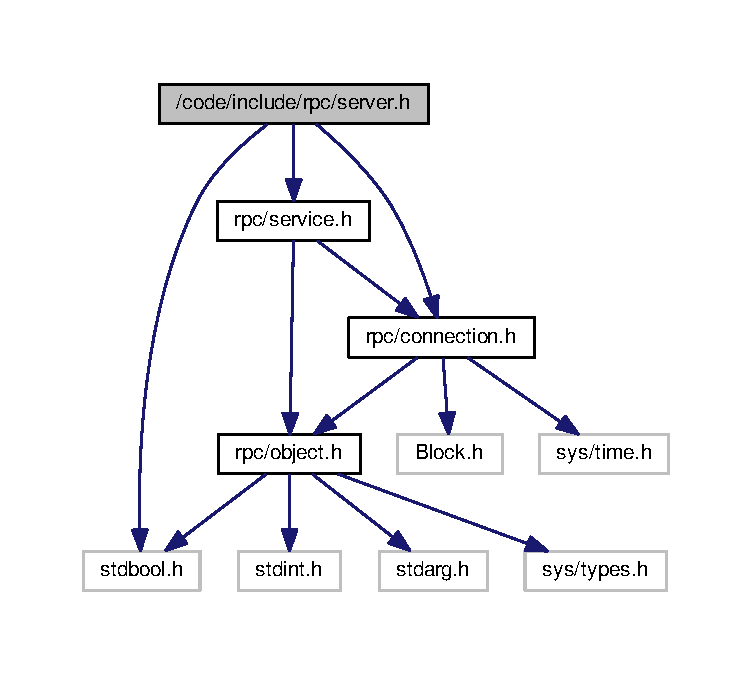
\includegraphics[width=350pt]{server_8h__incl}
\end{center}
\end{figure}
\subsection*{Macros}
\begin{DoxyCompactItemize}
\item 
\#define \hyperlink{server_8h_a34749fc2472ddb06c6d36006e2a948c3}{R\+P\+C\+\_\+\+S\+E\+R\+V\+E\+R\+\_\+\+H\+A\+N\+D\+L\+ER}(\+\_\+fn,  \+\_\+arg)
\end{DoxyCompactItemize}
\subsection*{Typedefs}
\begin{DoxyCompactItemize}
\item 
typedef struct rpc\+\_\+server $\ast$ \hyperlink{server_8h_a46fd27cbcf75a54103df9d51d90a7fca}{rpc\+\_\+server\+\_\+t}
\item 
typedef void($^\wedge$ \hyperlink{server_8h_a2d9a540637c63449db9ac5882cb5f7ab}{rpc\+\_\+server\+\_\+event\+\_\+handler\+\_\+t}) (\+\_\+\+Nonnull \hyperlink{connection_8h_a70838cb106c3464db299522c5fe2782d}{rpc\+\_\+connection\+\_\+t} source, const char $\ast$\+\_\+\+Nonnull name, \+\_\+\+Nonnull \hyperlink{object_8h_ab365f726b4975c0c8376b808d111d01b}{rpc\+\_\+object\+\_\+t} args)
\end{DoxyCompactItemize}
\subsection*{Functions}
\begin{DoxyCompactItemize}
\item 
\+\_\+\+Nullable \hyperlink{server_8h_a46fd27cbcf75a54103df9d51d90a7fca}{rpc\+\_\+server\+\_\+t} \hyperlink{server_8h_a74af7bf809de8e773b35038107db1221}{rpc\+\_\+server\+\_\+find} (const char $\ast$\+\_\+\+Nonnull uri, \+\_\+\+Nonnull \hyperlink{service_8h_a55087f28cb63ff45b6c798a5dabaedd7}{rpc\+\_\+context\+\_\+t} context)
\item 
\+\_\+\+Nullable \hyperlink{server_8h_a46fd27cbcf75a54103df9d51d90a7fca}{rpc\+\_\+server\+\_\+t} \hyperlink{server_8h_a2d524c3d5822d34b46f1d8552bf7ede0}{rpc\+\_\+server\+\_\+create} (const char $\ast$\+\_\+\+Nonnull uri, \+\_\+\+Nonnull \hyperlink{service_8h_a55087f28cb63ff45b6c798a5dabaedd7}{rpc\+\_\+context\+\_\+t} context)
\item 
void \hyperlink{server_8h_a7692f4863bf4db19759d95c132e03e61}{rpc\+\_\+server\+\_\+pause} (\+\_\+\+Nonnull \hyperlink{server_8h_a46fd27cbcf75a54103df9d51d90a7fca}{rpc\+\_\+server\+\_\+t} server)
\item 
void \hyperlink{server_8h_a52667e1f1ad29521541c60aae34dcf02}{rpc\+\_\+server\+\_\+resume} (\+\_\+\+Nonnull \hyperlink{server_8h_a46fd27cbcf75a54103df9d51d90a7fca}{rpc\+\_\+server\+\_\+t} server)
\item 
void \hyperlink{server_8h_a28eeff2b8ec73f31f1af9feff11cb698}{rpc\+\_\+server\+\_\+broadcast\+\_\+event} (\+\_\+\+Nonnull \hyperlink{server_8h_a46fd27cbcf75a54103df9d51d90a7fca}{rpc\+\_\+server\+\_\+t} server, const char $\ast$\+\_\+\+Nullable path, const char $\ast$\+\_\+\+Nullable interface, const char $\ast$\+\_\+\+Nonnull name, \+\_\+\+Nullable \hyperlink{object_8h_ab365f726b4975c0c8376b808d111d01b}{rpc\+\_\+object\+\_\+t} args)
\item 
void \hyperlink{server_8h_ac6bfcd59fe8ec8386b1e3d312705e786}{rpc\+\_\+server\+\_\+set\+\_\+event\+\_\+handler} (\+\_\+\+Nullable \hyperlink{server_8h_a2d9a540637c63449db9ac5882cb5f7ab}{rpc\+\_\+server\+\_\+event\+\_\+handler\+\_\+t} handler)
\item 
int \hyperlink{server_8h_a1bf6070b1bb3b31d394f3862405eaf8c}{rpc\+\_\+server\+\_\+close} (\+\_\+\+Nonnull \hyperlink{server_8h_a46fd27cbcf75a54103df9d51d90a7fca}{rpc\+\_\+server\+\_\+t} server)
\end{DoxyCompactItemize}


\subsection{Detailed Description}
R\+PC server A\+PI. 

\subsection{Macro Definition Documentation}
\mbox{\Hypertarget{server_8h_a34749fc2472ddb06c6d36006e2a948c3}\label{server_8h_a34749fc2472ddb06c6d36006e2a948c3}} 
\index{server.\+h@{server.\+h}!R\+P\+C\+\_\+\+S\+E\+R\+V\+E\+R\+\_\+\+H\+A\+N\+D\+L\+ER@{R\+P\+C\+\_\+\+S\+E\+R\+V\+E\+R\+\_\+\+H\+A\+N\+D\+L\+ER}}
\index{R\+P\+C\+\_\+\+S\+E\+R\+V\+E\+R\+\_\+\+H\+A\+N\+D\+L\+ER@{R\+P\+C\+\_\+\+S\+E\+R\+V\+E\+R\+\_\+\+H\+A\+N\+D\+L\+ER}!server.\+h@{server.\+h}}
\subsubsection{\texorpdfstring{R\+P\+C\+\_\+\+S\+E\+R\+V\+E\+R\+\_\+\+H\+A\+N\+D\+L\+ER}{RPC\_SERVER\_HANDLER}}
{\footnotesize\ttfamily \#define R\+P\+C\+\_\+\+S\+E\+R\+V\+E\+R\+\_\+\+H\+A\+N\+D\+L\+ER(\begin{DoxyParamCaption}\item[{}]{\+\_\+fn,  }\item[{}]{\+\_\+arg }\end{DoxyParamCaption})}

{\bfseries Value\+:}
\begin{DoxyCode}
^(\hyperlink{connection_8h_a70838cb106c3464db299522c5fe2782d}{rpc\_connection\_t} \_source, \textcolor{keyword}{const} \textcolor{keywordtype}{char} *\_name, \hyperlink{object_8h_ab365f726b4975c0c8376b808d111d01b}{rpc\_object\_t} \_args) \{    \(\backslash\)
        \_fn(\_arg, \_source, \_name, \_args);               \(\backslash\)
    \}
\end{DoxyCode}
Converts function pointer to a \hyperlink{server_8h_a2d9a540637c63449db9ac5882cb5f7ab}{rpc\+\_\+server\+\_\+event\+\_\+handler\+\_\+t} block type. 

Definition at line 64 of file server.\+h.



\subsection{Typedef Documentation}
\mbox{\Hypertarget{server_8h_a2d9a540637c63449db9ac5882cb5f7ab}\label{server_8h_a2d9a540637c63449db9ac5882cb5f7ab}} 
\index{server.\+h@{server.\+h}!rpc\+\_\+server\+\_\+event\+\_\+handler\+\_\+t@{rpc\+\_\+server\+\_\+event\+\_\+handler\+\_\+t}}
\index{rpc\+\_\+server\+\_\+event\+\_\+handler\+\_\+t@{rpc\+\_\+server\+\_\+event\+\_\+handler\+\_\+t}!server.\+h@{server.\+h}}
\subsubsection{\texorpdfstring{rpc\+\_\+server\+\_\+event\+\_\+handler\+\_\+t}{rpc\_server\_event\_handler\_t}}
{\footnotesize\ttfamily typedef void($^\wedge$ rpc\+\_\+server\+\_\+event\+\_\+handler\+\_\+t) (\+\_\+\+Nonnull \hyperlink{connection_8h_a70838cb106c3464db299522c5fe2782d}{rpc\+\_\+connection\+\_\+t} source, const char $\ast$\+\_\+\+Nonnull name, \+\_\+\+Nonnull \hyperlink{object_8h_ab365f726b4975c0c8376b808d111d01b}{rpc\+\_\+object\+\_\+t} args)}

Definition of R\+PC server event handler block type. 

Definition at line 58 of file server.\+h.

\mbox{\Hypertarget{server_8h_a46fd27cbcf75a54103df9d51d90a7fca}\label{server_8h_a46fd27cbcf75a54103df9d51d90a7fca}} 
\index{server.\+h@{server.\+h}!rpc\+\_\+server\+\_\+t@{rpc\+\_\+server\+\_\+t}}
\index{rpc\+\_\+server\+\_\+t@{rpc\+\_\+server\+\_\+t}!server.\+h@{server.\+h}}
\subsubsection{\texorpdfstring{rpc\+\_\+server\+\_\+t}{rpc\_server\_t}}
{\footnotesize\ttfamily typedef struct rpc\+\_\+server$\ast$ \hyperlink{server_8h_a46fd27cbcf75a54103df9d51d90a7fca}{rpc\+\_\+server\+\_\+t}}

R\+PC server pointer structure definition. 

Definition at line 53 of file server.\+h.



\subsection{Function Documentation}
\mbox{\Hypertarget{server_8h_a28eeff2b8ec73f31f1af9feff11cb698}\label{server_8h_a28eeff2b8ec73f31f1af9feff11cb698}} 
\index{server.\+h@{server.\+h}!rpc\+\_\+server\+\_\+broadcast\+\_\+event@{rpc\+\_\+server\+\_\+broadcast\+\_\+event}}
\index{rpc\+\_\+server\+\_\+broadcast\+\_\+event@{rpc\+\_\+server\+\_\+broadcast\+\_\+event}!server.\+h@{server.\+h}}
\subsubsection{\texorpdfstring{rpc\+\_\+server\+\_\+broadcast\+\_\+event()}{rpc\_server\_broadcast\_event()}}
{\footnotesize\ttfamily void rpc\+\_\+server\+\_\+broadcast\+\_\+event (\begin{DoxyParamCaption}\item[{\+\_\+\+Nonnull \hyperlink{server_8h_a46fd27cbcf75a54103df9d51d90a7fca}{rpc\+\_\+server\+\_\+t}}]{server,  }\item[{const char $\ast$\+\_\+\+Nullable}]{path,  }\item[{const char $\ast$\+\_\+\+Nullable}]{interface,  }\item[{const char $\ast$\+\_\+\+Nonnull}]{name,  }\item[{\+\_\+\+Nullable \hyperlink{object_8h_ab365f726b4975c0c8376b808d111d01b}{rpc\+\_\+object\+\_\+t}}]{args }\end{DoxyParamCaption})}

Broadcasts an event of a given name among its subscribers.


\begin{DoxyParams}{Parameters}
{\em server} & Server handle \\
\hline
{\em name} & Name of an event to be broadcasted \\
\hline
{\em args} & Event arguments \\
\hline
\end{DoxyParams}
\mbox{\Hypertarget{server_8h_a1bf6070b1bb3b31d394f3862405eaf8c}\label{server_8h_a1bf6070b1bb3b31d394f3862405eaf8c}} 
\index{server.\+h@{server.\+h}!rpc\+\_\+server\+\_\+close@{rpc\+\_\+server\+\_\+close}}
\index{rpc\+\_\+server\+\_\+close@{rpc\+\_\+server\+\_\+close}!server.\+h@{server.\+h}}
\subsubsection{\texorpdfstring{rpc\+\_\+server\+\_\+close()}{rpc\_server\_close()}}
{\footnotesize\ttfamily int rpc\+\_\+server\+\_\+close (\begin{DoxyParamCaption}\item[{\+\_\+\+Nonnull \hyperlink{server_8h_a46fd27cbcf75a54103df9d51d90a7fca}{rpc\+\_\+server\+\_\+t}}]{server }\end{DoxyParamCaption})}

Closes a given R\+PC server.


\begin{DoxyParams}{Parameters}
{\em server} & Server handle to be closed \\
\hline
\end{DoxyParams}
\begin{DoxyReturn}{Returns}
0 on successful teardown 
\end{DoxyReturn}
\mbox{\Hypertarget{server_8h_a2d524c3d5822d34b46f1d8552bf7ede0}\label{server_8h_a2d524c3d5822d34b46f1d8552bf7ede0}} 
\index{server.\+h@{server.\+h}!rpc\+\_\+server\+\_\+create@{rpc\+\_\+server\+\_\+create}}
\index{rpc\+\_\+server\+\_\+create@{rpc\+\_\+server\+\_\+create}!server.\+h@{server.\+h}}
\subsubsection{\texorpdfstring{rpc\+\_\+server\+\_\+create()}{rpc\_server\_create()}}
{\footnotesize\ttfamily \+\_\+\+Nullable \hyperlink{server_8h_a46fd27cbcf75a54103df9d51d90a7fca}{rpc\+\_\+server\+\_\+t} rpc\+\_\+server\+\_\+create (\begin{DoxyParamCaption}\item[{const char $\ast$\+\_\+\+Nonnull}]{uri,  }\item[{\+\_\+\+Nonnull \hyperlink{service_8h_a55087f28cb63ff45b6c798a5dabaedd7}{rpc\+\_\+context\+\_\+t}}]{context }\end{DoxyParamCaption})}

Creates a server instance listening on a given U\+RI.


\begin{DoxyParams}{Parameters}
{\em uri} & U\+RI to listen on \\
\hline
{\em context} & R\+PC context for a server instance \\
\hline
\end{DoxyParams}
\begin{DoxyReturn}{Returns}
Server handle 
\end{DoxyReturn}
\mbox{\Hypertarget{server_8h_a74af7bf809de8e773b35038107db1221}\label{server_8h_a74af7bf809de8e773b35038107db1221}} 
\index{server.\+h@{server.\+h}!rpc\+\_\+server\+\_\+find@{rpc\+\_\+server\+\_\+find}}
\index{rpc\+\_\+server\+\_\+find@{rpc\+\_\+server\+\_\+find}!server.\+h@{server.\+h}}
\subsubsection{\texorpdfstring{rpc\+\_\+server\+\_\+find()}{rpc\_server\_find()}}
{\footnotesize\ttfamily \+\_\+\+Nullable \hyperlink{server_8h_a46fd27cbcf75a54103df9d51d90a7fca}{rpc\+\_\+server\+\_\+t} rpc\+\_\+server\+\_\+find (\begin{DoxyParamCaption}\item[{const char $\ast$\+\_\+\+Nonnull}]{uri,  }\item[{\+\_\+\+Nonnull \hyperlink{service_8h_a55087f28cb63ff45b6c798a5dabaedd7}{rpc\+\_\+context\+\_\+t}}]{context }\end{DoxyParamCaption})}

Returns the server handle of the supplied U\+RI if such a server exists on the context.


\begin{DoxyParams}{Parameters}
{\em uri} & U\+RI for the context search \\
\hline
{\em context} & R\+PC context for a server instance \\
\hline
\end{DoxyParams}
\begin{DoxyReturn}{Returns}
the handle if a server with the U\+RI exists, else N\+U\+LL 
\end{DoxyReturn}
\mbox{\Hypertarget{server_8h_a7692f4863bf4db19759d95c132e03e61}\label{server_8h_a7692f4863bf4db19759d95c132e03e61}} 
\index{server.\+h@{server.\+h}!rpc\+\_\+server\+\_\+pause@{rpc\+\_\+server\+\_\+pause}}
\index{rpc\+\_\+server\+\_\+pause@{rpc\+\_\+server\+\_\+pause}!server.\+h@{server.\+h}}
\subsubsection{\texorpdfstring{rpc\+\_\+server\+\_\+pause()}{rpc\_server\_pause()}}
{\footnotesize\ttfamily void rpc\+\_\+server\+\_\+pause (\begin{DoxyParamCaption}\item[{\+\_\+\+Nonnull \hyperlink{server_8h_a46fd27cbcf75a54103df9d51d90a7fca}{rpc\+\_\+server\+\_\+t}}]{server }\end{DoxyParamCaption})}

Stops accepting requests for the server.

Server instance keeps all the incoming requests queued and on hold until \hyperlink{server_8h_a52667e1f1ad29521541c60aae34dcf02}{rpc\+\_\+server\+\_\+resume} is called.


\begin{DoxyParams}{Parameters}
{\em server} & Server handle \\
\hline
\end{DoxyParams}
\mbox{\Hypertarget{server_8h_a52667e1f1ad29521541c60aae34dcf02}\label{server_8h_a52667e1f1ad29521541c60aae34dcf02}} 
\index{server.\+h@{server.\+h}!rpc\+\_\+server\+\_\+resume@{rpc\+\_\+server\+\_\+resume}}
\index{rpc\+\_\+server\+\_\+resume@{rpc\+\_\+server\+\_\+resume}!server.\+h@{server.\+h}}
\subsubsection{\texorpdfstring{rpc\+\_\+server\+\_\+resume()}{rpc\_server\_resume()}}
{\footnotesize\ttfamily void rpc\+\_\+server\+\_\+resume (\begin{DoxyParamCaption}\item[{\+\_\+\+Nonnull \hyperlink{server_8h_a46fd27cbcf75a54103df9d51d90a7fca}{rpc\+\_\+server\+\_\+t}}]{server }\end{DoxyParamCaption})}

Starts accepting requests by the server.

Server instance keeps all the incoming requests queued and on hold until this function is called.


\begin{DoxyParams}{Parameters}
{\em server} & Server handle \\
\hline
\end{DoxyParams}
\mbox{\Hypertarget{server_8h_ac6bfcd59fe8ec8386b1e3d312705e786}\label{server_8h_ac6bfcd59fe8ec8386b1e3d312705e786}} 
\index{server.\+h@{server.\+h}!rpc\+\_\+server\+\_\+set\+\_\+event\+\_\+handler@{rpc\+\_\+server\+\_\+set\+\_\+event\+\_\+handler}}
\index{rpc\+\_\+server\+\_\+set\+\_\+event\+\_\+handler@{rpc\+\_\+server\+\_\+set\+\_\+event\+\_\+handler}!server.\+h@{server.\+h}}
\subsubsection{\texorpdfstring{rpc\+\_\+server\+\_\+set\+\_\+event\+\_\+handler()}{rpc\_server\_set\_event\_handler()}}
{\footnotesize\ttfamily void rpc\+\_\+server\+\_\+set\+\_\+event\+\_\+handler (\begin{DoxyParamCaption}\item[{\+\_\+\+Nullable \hyperlink{server_8h_a2d9a540637c63449db9ac5882cb5f7ab}{rpc\+\_\+server\+\_\+event\+\_\+handler\+\_\+t}}]{handler }\end{DoxyParamCaption})}

Creates an event handler internal to a server for an event of a given name.


\begin{DoxyParams}{Parameters}
{\em handler} & \\
\hline
\end{DoxyParams}

\hypertarget{service_8h}{}\section{/code/include/rpc/service.h File Reference}
\label{service_8h}\index{/code/include/rpc/service.\+h@{/code/include/rpc/service.\+h}}
{\ttfamily \#include $<$rpc/object.\+h$>$}\\*
{\ttfamily \#include $<$rpc/connection.\+h$>$}\\*
Include dependency graph for service.\+h\+:
\nopagebreak
\begin{figure}[H]
\begin{center}
\leavevmode
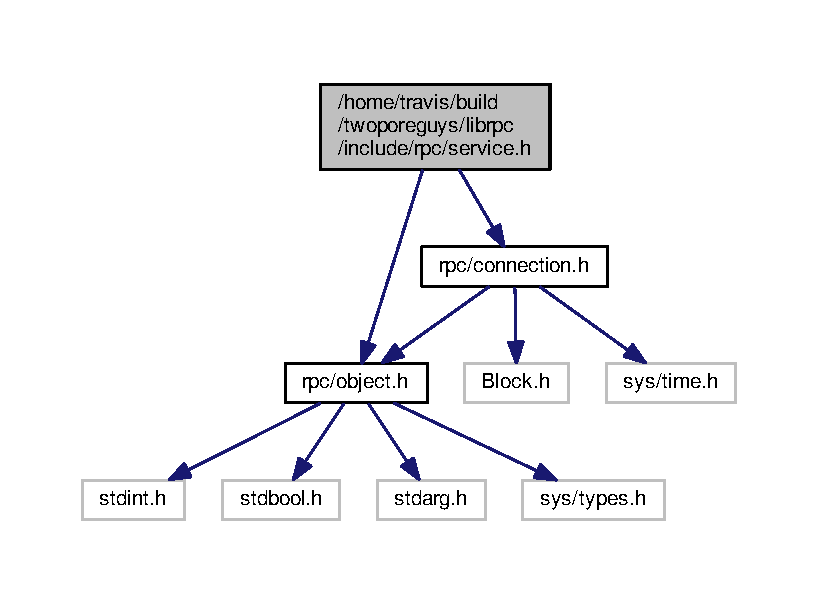
\includegraphics[width=350pt]{service_8h__incl}
\end{center}
\end{figure}
This graph shows which files directly or indirectly include this file\+:
\nopagebreak
\begin{figure}[H]
\begin{center}
\leavevmode
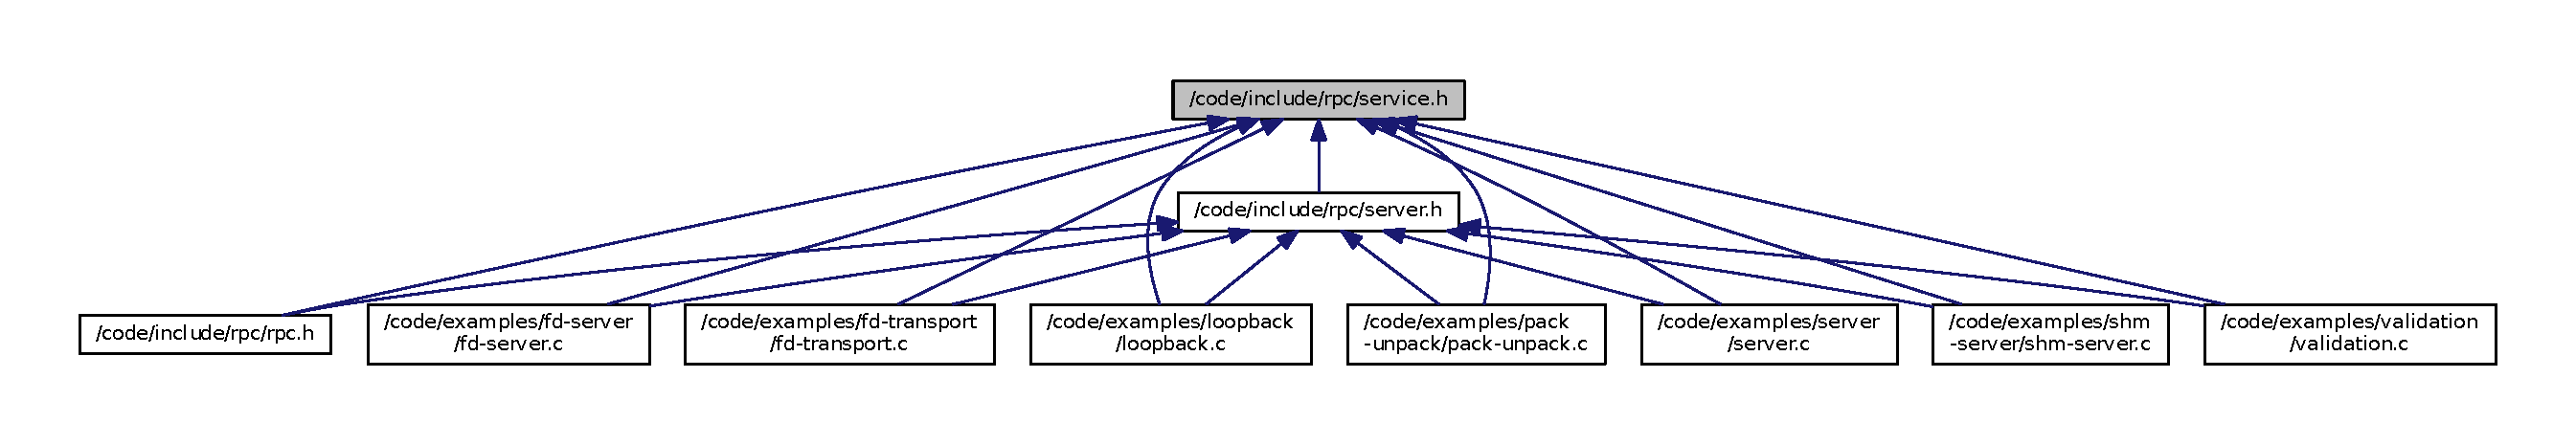
\includegraphics[width=350pt]{service_8h__dep__incl}
\end{center}
\end{figure}
\subsection*{Classes}
\begin{DoxyCompactItemize}
\item 
struct \hyperlink{structrpc__method}{rpc\+\_\+method}
\end{DoxyCompactItemize}
\subsection*{Macros}
\begin{DoxyCompactItemize}
\item 
\#define {\bfseries R\+P\+C\+\_\+\+F\+U\+N\+C\+T\+I\+O\+N\+\_\+\+S\+T\+I\+L\+L\+\_\+\+R\+U\+N\+N\+I\+NG}~((\hyperlink{object_8h_ab365f726b4975c0c8376b808d111d01b}{rpc\+\_\+object\+\_\+t})1)\hypertarget{service_8h_a4c7094875a0bd8cc87e7c1d24a4481a6}{}\label{service_8h_a4c7094875a0bd8cc87e7c1d24a4481a6}

\end{DoxyCompactItemize}
\subsection*{Typedefs}
\begin{DoxyCompactItemize}
\item 
typedef struct rpc\+\_\+context $\ast$ \hyperlink{service_8h_a55087f28cb63ff45b6c798a5dabaedd7}{rpc\+\_\+context\+\_\+t}
\item 
typedef struct rpc\+\_\+instance $\ast$ {\bfseries rpc\+\_\+instance\+\_\+t}\hypertarget{service_8h_afd1294bd7ea02592ecc002e1576ef290}{}\label{service_8h_afd1294bd7ea02592ecc002e1576ef290}

\item 
typedef \hyperlink{object_8h_ab365f726b4975c0c8376b808d111d01b}{rpc\+\_\+object\+\_\+t}($^\wedge$ \hyperlink{service_8h_a02d3dbd723de9bd5140887c9935ff05a}{rpc\+\_\+function\+\_\+t}) (void $\ast$cookie, \hyperlink{object_8h_ab365f726b4975c0c8376b808d111d01b}{rpc\+\_\+object\+\_\+t} args)
\item 
typedef \hyperlink{object_8h_ab365f726b4975c0c8376b808d111d01b}{rpc\+\_\+object\+\_\+t}($\ast$ \hyperlink{service_8h_a1f67d69a108ffc8087346616d82eacf7}{rpc\+\_\+function\+\_\+f}) (void $\ast$cookie, \hyperlink{object_8h_ab365f726b4975c0c8376b808d111d01b}{rpc\+\_\+object\+\_\+t} args)
\end{DoxyCompactItemize}
\subsection*{Functions}
\begin{DoxyCompactItemize}
\item 
\hyperlink{service_8h_a55087f28cb63ff45b6c798a5dabaedd7}{rpc\+\_\+context\+\_\+t} \hyperlink{service_8h_a2f099d270db1d46696878337c20d1bdd}{rpc\+\_\+context\+\_\+create} (void)
\item 
void \hyperlink{service_8h_ae62c27a53aea99a9c87e5b12b3d3cbbc}{rpc\+\_\+context\+\_\+free} (\hyperlink{service_8h_a55087f28cb63ff45b6c798a5dabaedd7}{rpc\+\_\+context\+\_\+t} context)
\item 
rpc\+\_\+instance\+\_\+t \hyperlink{service_8h_a20f26ce7e4fd8d1a81f8bb616939dec7}{rpc\+\_\+context\+\_\+find\+\_\+instance} (\hyperlink{service_8h_a55087f28cb63ff45b6c798a5dabaedd7}{rpc\+\_\+context\+\_\+t} context, const char $\ast$path)
\item 
rpc\+\_\+instance\+\_\+t \hyperlink{service_8h_a9b55b5c3cd7c1f3de1755f8b287ee6db}{rpc\+\_\+context\+\_\+get\+\_\+root} (\hyperlink{service_8h_a55087f28cb63ff45b6c798a5dabaedd7}{rpc\+\_\+context\+\_\+t} context)
\item 
int \hyperlink{service_8h_a8357a5f08304aadf30fbc05fd625ea86}{rpc\+\_\+context\+\_\+register\+\_\+instance} (\hyperlink{service_8h_a55087f28cb63ff45b6c798a5dabaedd7}{rpc\+\_\+context\+\_\+t} context, const char $\ast$path, rpc\+\_\+instance\+\_\+t instance)
\item 
int \hyperlink{service_8h_abd3ce744fe6091cf188b1f44b31548da}{rpc\+\_\+context\+\_\+register\+\_\+method} (\hyperlink{service_8h_a55087f28cb63ff45b6c798a5dabaedd7}{rpc\+\_\+context\+\_\+t} context, struct \hyperlink{structrpc__method}{rpc\+\_\+method} $\ast$m)
\item 
int \hyperlink{service_8h_af83b298b11aec4f97c0db5d4391b0be7}{rpc\+\_\+context\+\_\+register\+\_\+block} (\hyperlink{service_8h_a55087f28cb63ff45b6c798a5dabaedd7}{rpc\+\_\+context\+\_\+t} context, const char $\ast$name, const char $\ast$descr, void $\ast$arg, \hyperlink{service_8h_a02d3dbd723de9bd5140887c9935ff05a}{rpc\+\_\+function\+\_\+t} func)
\item 
int \hyperlink{service_8h_a6de78771a848fe3b2001e08a7cf0a88c}{rpc\+\_\+context\+\_\+register\+\_\+func} (\hyperlink{service_8h_a55087f28cb63ff45b6c798a5dabaedd7}{rpc\+\_\+context\+\_\+t} context, const char $\ast$name, const char $\ast$descr, void $\ast$arg, \hyperlink{service_8h_a1f67d69a108ffc8087346616d82eacf7}{rpc\+\_\+function\+\_\+f} func)
\item 
int \hyperlink{service_8h_a8c96adc49c6ecf3c0ad7ae1ad7c82411}{rpc\+\_\+context\+\_\+unregister\+\_\+method} (\hyperlink{service_8h_a55087f28cb63ff45b6c798a5dabaedd7}{rpc\+\_\+context\+\_\+t} context, const char $\ast$interface, const char $\ast$name)
\item 
void \hyperlink{service_8h_ad1c0c9c7897adf4ad5e7ee9c40e545b8}{rpc\+\_\+context\+\_\+set\+\_\+pre\+\_\+call\+\_\+hook} (\hyperlink{service_8h_a55087f28cb63ff45b6c798a5dabaedd7}{rpc\+\_\+context\+\_\+t} context, \hyperlink{service_8h_a02d3dbd723de9bd5140887c9935ff05a}{rpc\+\_\+function\+\_\+t} fn)
\item 
void \hyperlink{service_8h_a36c5dae2cc75f5d4a740c5db25e25d7a}{rpc\+\_\+context\+\_\+set\+\_\+post\+\_\+call\+\_\+hook} (\hyperlink{service_8h_a55087f28cb63ff45b6c798a5dabaedd7}{rpc\+\_\+context\+\_\+t} context, \hyperlink{service_8h_a02d3dbd723de9bd5140887c9935ff05a}{rpc\+\_\+function\+\_\+t} fn)
\item 
\hyperlink{connection_8h_aeb6f25e395cc04930537960ef6b50106}{rpc\+\_\+call\+\_\+t} \hyperlink{service_8h_a206fab24804db208f9b4d44f4c303596}{rpc\+\_\+context\+\_\+dispatch\+\_\+call} (\hyperlink{service_8h_a55087f28cb63ff45b6c798a5dabaedd7}{rpc\+\_\+context\+\_\+t} context, const char $\ast$name, \hyperlink{object_8h_ab365f726b4975c0c8376b808d111d01b}{rpc\+\_\+object\+\_\+t} args)
\item 
void $\ast$ \hyperlink{service_8h_a62e71e6c0208e7ed1e23e2f9f3cd78f2}{rpc\+\_\+function\+\_\+get\+\_\+arg} (void $\ast$cookie)
\item 
\hyperlink{service_8h_a55087f28cb63ff45b6c798a5dabaedd7}{rpc\+\_\+context\+\_\+t} \hyperlink{service_8h_a51694182976cc6191bdd45205f027ca1}{rpc\+\_\+function\+\_\+get\+\_\+context} (void $\ast$cookie)
\item 
const char $\ast$ \hyperlink{service_8h_a0d57a21163cd2d8bd06add360270809c}{rpc\+\_\+function\+\_\+get\+\_\+name} (void $\ast$cookie)
\item 
const char $\ast$ \hyperlink{service_8h_a6617fa9bcafd942255e9ec3bd9ecbf1e}{rpc\+\_\+function\+\_\+get\+\_\+path} (void $\ast$cookie)
\item 
const char $\ast$ \hyperlink{service_8h_a51e6cad2e4f70b1a073e54a323064420}{rpc\+\_\+function\+\_\+get\+\_\+interface} (void $\ast$cookie)
\item 
void \hyperlink{service_8h_a1b73c8714198994d5055bf5cfe3012a4}{rpc\+\_\+function\+\_\+respond} (void $\ast$cookie, \hyperlink{object_8h_ab365f726b4975c0c8376b808d111d01b}{rpc\+\_\+object\+\_\+t} object)
\item 
void \hyperlink{service_8h_ad7d639f2063a65279f159175a473b881}{rpc\+\_\+function\+\_\+error} (void $\ast$cookie, int code, const char $\ast$message,...)
\item 
void \hyperlink{service_8h_acfe4732dbbfa89a8b2972e80b6d65de1}{rpc\+\_\+function\+\_\+error\+\_\+ex} (void $\ast$cookie, \hyperlink{object_8h_ab365f726b4975c0c8376b808d111d01b}{rpc\+\_\+object\+\_\+t} exception)
\item 
int \hyperlink{service_8h_a36b4ff5a09f3a8139f1d5b59ab930139}{rpc\+\_\+function\+\_\+yield} (void $\ast$cookie, \hyperlink{object_8h_ab365f726b4975c0c8376b808d111d01b}{rpc\+\_\+object\+\_\+t} fragment)
\item 
void \hyperlink{service_8h_a7e912e42af9c3899e74e1ef539ca7e50}{rpc\+\_\+function\+\_\+end} (void $\ast$cookie)
\item 
bool \hyperlink{service_8h_a23fb9149cf7ad5bfdec4bc24fd805617}{rpc\+\_\+function\+\_\+should\+\_\+abort} (void $\ast$cookie)
\item 
rpc\+\_\+instance\+\_\+t \hyperlink{service_8h_a3ec7513dc05be23e71fe2fbdf134b478}{rpc\+\_\+instance\+\_\+new} (const char $\ast$path, void $\ast$arg)
\item 
void $\ast$ \hyperlink{service_8h_a6f4eb6df2553bf05ce15f74950f6415e}{rpc\+\_\+instance\+\_\+get\+\_\+arg} (rpc\+\_\+instance\+\_\+t instance)
\item 
const char $\ast$ \hyperlink{service_8h_a68b61823da7220e591aa5b815fe5cc5e}{rpc\+\_\+instance\+\_\+get\+\_\+path} (rpc\+\_\+instance\+\_\+t instance)
\item 
int \hyperlink{service_8h_a1903baa0815e6ed639178888cd81b2b3}{rpc\+\_\+instance\+\_\+register\+\_\+method} (rpc\+\_\+instance\+\_\+t instance, struct \hyperlink{structrpc__method}{rpc\+\_\+method} $\ast$m)
\item 
int \hyperlink{service_8h_afa0f59ae87c130966ba378bc6c2ee12b}{rpc\+\_\+instance\+\_\+register\+\_\+block} (rpc\+\_\+instance\+\_\+t instance, const char $\ast$interface, const char $\ast$name, void $\ast$arg, \hyperlink{service_8h_a02d3dbd723de9bd5140887c9935ff05a}{rpc\+\_\+function\+\_\+t} fn)
\item 
int \hyperlink{service_8h_ad5db3e98c350f755011b6d470ba21373}{rpc\+\_\+instance\+\_\+register\+\_\+func} (rpc\+\_\+instance\+\_\+t instance, const char $\ast$interface, const char $\ast$name, void $\ast$arg, \hyperlink{service_8h_a1f67d69a108ffc8087346616d82eacf7}{rpc\+\_\+function\+\_\+f} fn)
\item 
int \hyperlink{service_8h_a76cbc7eebe61d4fedf608d4f411cacba}{rpc\+\_\+instance\+\_\+unregister\+\_\+method} (rpc\+\_\+instance\+\_\+t instance, const char $\ast$interface, const char $\ast$name)
\item 
struct \hyperlink{structrpc__method}{rpc\+\_\+method} $\ast$ \hyperlink{service_8h_a73d9c76529ba51d29880464c415db845}{rpc\+\_\+instance\+\_\+find\+\_\+method} (rpc\+\_\+instance\+\_\+t instance, const char $\ast$interface, const char $\ast$name)
\item 
void \hyperlink{service_8h_ae95d9adc6b892e610116469623589727}{rpc\+\_\+instance\+\_\+emit\+\_\+event} (rpc\+\_\+instance\+\_\+t instance, const char $\ast$interface, const char $\ast$name)
\item 
void \hyperlink{service_8h_a5ff30bf1b1536f88fe0946c5df4359bd}{rpc\+\_\+instance\+\_\+free} (rpc\+\_\+instance\+\_\+t instance)
\item 
int \hyperlink{service_8h_a2d3e19a87010024c5c49a6620cf280bf}{rpc\+\_\+instance\+\_\+register} (\hyperlink{service_8h_a55087f28cb63ff45b6c798a5dabaedd7}{rpc\+\_\+context\+\_\+t} context, rpc\+\_\+instance\+\_\+t instance)
\item 
int \hyperlink{service_8h_a3dbca2ed6c2f7479b286b62677cfa9d1}{rpc\+\_\+instance\+\_\+unregister} (const char $\ast$path)
\end{DoxyCompactItemize}


\subsection{Detailed Description}
R\+PC service A\+PI. 

\subsection{Typedef Documentation}
\index{service.\+h@{service.\+h}!rpc\+\_\+context\+\_\+t@{rpc\+\_\+context\+\_\+t}}
\index{rpc\+\_\+context\+\_\+t@{rpc\+\_\+context\+\_\+t}!service.\+h@{service.\+h}}
\subsubsection[{\texorpdfstring{rpc\+\_\+context\+\_\+t}{rpc_context_t}}]{\setlength{\rightskip}{0pt plus 5cm}typedef struct rpc\+\_\+context$\ast$ {\bf rpc\+\_\+context\+\_\+t}}\hypertarget{service_8h_a55087f28cb63ff45b6c798a5dabaedd7}{}\label{service_8h_a55087f28cb63ff45b6c798a5dabaedd7}
R\+PC context structure pointer definition. 

Definition at line 55 of file service.\+h.

\index{service.\+h@{service.\+h}!rpc\+\_\+function\+\_\+f@{rpc\+\_\+function\+\_\+f}}
\index{rpc\+\_\+function\+\_\+f@{rpc\+\_\+function\+\_\+f}!service.\+h@{service.\+h}}
\subsubsection[{\texorpdfstring{rpc\+\_\+function\+\_\+f}{rpc_function_f}}]{\setlength{\rightskip}{0pt plus 5cm}typedef {\bf rpc\+\_\+object\+\_\+t}($\ast$ rpc\+\_\+function\+\_\+f) (void $\ast$cookie, {\bf rpc\+\_\+object\+\_\+t} args)}\hypertarget{service_8h_a1f67d69a108ffc8087346616d82eacf7}{}\label{service_8h_a1f67d69a108ffc8087346616d82eacf7}
Definition of R\+PC method function type. 

Definition at line 68 of file service.\+h.

\index{service.\+h@{service.\+h}!rpc\+\_\+function\+\_\+t@{rpc\+\_\+function\+\_\+t}}
\index{rpc\+\_\+function\+\_\+t@{rpc\+\_\+function\+\_\+t}!service.\+h@{service.\+h}}
\subsubsection[{\texorpdfstring{rpc\+\_\+function\+\_\+t}{rpc_function_t}}]{\setlength{\rightskip}{0pt plus 5cm}typedef {\bf rpc\+\_\+object\+\_\+t}($^\wedge$ rpc\+\_\+function\+\_\+t) (void $\ast$cookie, {\bf rpc\+\_\+object\+\_\+t} args)}\hypertarget{service_8h_a02d3dbd723de9bd5140887c9935ff05a}{}\label{service_8h_a02d3dbd723de9bd5140887c9935ff05a}
Definition of R\+PC method block type. 

Definition at line 63 of file service.\+h.



\subsection{Function Documentation}
\index{service.\+h@{service.\+h}!rpc\+\_\+context\+\_\+create@{rpc\+\_\+context\+\_\+create}}
\index{rpc\+\_\+context\+\_\+create@{rpc\+\_\+context\+\_\+create}!service.\+h@{service.\+h}}
\subsubsection[{\texorpdfstring{rpc\+\_\+context\+\_\+create(void)}{rpc_context_create(void)}}]{\setlength{\rightskip}{0pt plus 5cm}{\bf rpc\+\_\+context\+\_\+t} rpc\+\_\+context\+\_\+create (
\begin{DoxyParamCaption}
\item[{void}]{}
\end{DoxyParamCaption}
)}\hypertarget{service_8h_a2f099d270db1d46696878337c20d1bdd}{}\label{service_8h_a2f099d270db1d46696878337c20d1bdd}
Creates a new R\+PC context.

\begin{DoxyReturn}{Returns}
Newly created R\+PC context object. 
\end{DoxyReturn}
\index{service.\+h@{service.\+h}!rpc\+\_\+context\+\_\+dispatch\+\_\+call@{rpc\+\_\+context\+\_\+dispatch\+\_\+call}}
\index{rpc\+\_\+context\+\_\+dispatch\+\_\+call@{rpc\+\_\+context\+\_\+dispatch\+\_\+call}!service.\+h@{service.\+h}}
\subsubsection[{\texorpdfstring{rpc\+\_\+context\+\_\+dispatch\+\_\+call(rpc\+\_\+context\+\_\+t context, const char $\ast$name, rpc\+\_\+object\+\_\+t args)}{rpc_context_dispatch_call(rpc_context_t context, const char *name, rpc_object_t args)}}]{\setlength{\rightskip}{0pt plus 5cm}{\bf rpc\+\_\+call\+\_\+t} rpc\+\_\+context\+\_\+dispatch\+\_\+call (
\begin{DoxyParamCaption}
\item[{{\bf rpc\+\_\+context\+\_\+t}}]{context, }
\item[{const char $\ast$}]{name, }
\item[{{\bf rpc\+\_\+object\+\_\+t}}]{args}
\end{DoxyParamCaption}
)}\hypertarget{service_8h_a206fab24804db208f9b4d44f4c303596}{}\label{service_8h_a206fab24804db208f9b4d44f4c303596}

\begin{DoxyParams}{Parameters}
{\em context} & \\
\hline
{\em name} & \\
\hline
{\em args} & \\
\hline
\end{DoxyParams}
\begin{DoxyReturn}{Returns}

\end{DoxyReturn}
\index{service.\+h@{service.\+h}!rpc\+\_\+context\+\_\+find\+\_\+instance@{rpc\+\_\+context\+\_\+find\+\_\+instance}}
\index{rpc\+\_\+context\+\_\+find\+\_\+instance@{rpc\+\_\+context\+\_\+find\+\_\+instance}!service.\+h@{service.\+h}}
\subsubsection[{\texorpdfstring{rpc\+\_\+context\+\_\+find\+\_\+instance(rpc\+\_\+context\+\_\+t context, const char $\ast$path)}{rpc_context_find_instance(rpc_context_t context, const char *path)}}]{\setlength{\rightskip}{0pt plus 5cm}rpc\+\_\+instance\+\_\+t rpc\+\_\+context\+\_\+find\+\_\+instance (
\begin{DoxyParamCaption}
\item[{{\bf rpc\+\_\+context\+\_\+t}}]{context, }
\item[{const char $\ast$}]{path}
\end{DoxyParamCaption}
)}\hypertarget{service_8h_a20f26ce7e4fd8d1a81f8bb616939dec7}{}\label{service_8h_a20f26ce7e4fd8d1a81f8bb616939dec7}

\begin{DoxyParams}{Parameters}
{\em context} & \\
\hline
{\em path} & \\
\hline
\end{DoxyParams}
\begin{DoxyReturn}{Returns}

\end{DoxyReturn}
\index{service.\+h@{service.\+h}!rpc\+\_\+context\+\_\+free@{rpc\+\_\+context\+\_\+free}}
\index{rpc\+\_\+context\+\_\+free@{rpc\+\_\+context\+\_\+free}!service.\+h@{service.\+h}}
\subsubsection[{\texorpdfstring{rpc\+\_\+context\+\_\+free(rpc\+\_\+context\+\_\+t context)}{rpc_context_free(rpc_context_t context)}}]{\setlength{\rightskip}{0pt plus 5cm}void rpc\+\_\+context\+\_\+free (
\begin{DoxyParamCaption}
\item[{{\bf rpc\+\_\+context\+\_\+t}}]{context}
\end{DoxyParamCaption}
)}\hypertarget{service_8h_ae62c27a53aea99a9c87e5b12b3d3cbbc}{}\label{service_8h_ae62c27a53aea99a9c87e5b12b3d3cbbc}
Disposes existing R\+PC context and frees all associated resources.


\begin{DoxyParams}{Parameters}
{\em context} & Context to dispose \\
\hline
\end{DoxyParams}
\index{service.\+h@{service.\+h}!rpc\+\_\+context\+\_\+get\+\_\+root@{rpc\+\_\+context\+\_\+get\+\_\+root}}
\index{rpc\+\_\+context\+\_\+get\+\_\+root@{rpc\+\_\+context\+\_\+get\+\_\+root}!service.\+h@{service.\+h}}
\subsubsection[{\texorpdfstring{rpc\+\_\+context\+\_\+get\+\_\+root(rpc\+\_\+context\+\_\+t context)}{rpc_context_get_root(rpc_context_t context)}}]{\setlength{\rightskip}{0pt plus 5cm}rpc\+\_\+instance\+\_\+t rpc\+\_\+context\+\_\+get\+\_\+root (
\begin{DoxyParamCaption}
\item[{{\bf rpc\+\_\+context\+\_\+t}}]{context}
\end{DoxyParamCaption}
)}\hypertarget{service_8h_a9b55b5c3cd7c1f3de1755f8b287ee6db}{}\label{service_8h_a9b55b5c3cd7c1f3de1755f8b287ee6db}

\begin{DoxyParams}{Parameters}
{\em context} & \\
\hline
\end{DoxyParams}
\begin{DoxyReturn}{Returns}

\end{DoxyReturn}
\index{service.\+h@{service.\+h}!rpc\+\_\+context\+\_\+register\+\_\+block@{rpc\+\_\+context\+\_\+register\+\_\+block}}
\index{rpc\+\_\+context\+\_\+register\+\_\+block@{rpc\+\_\+context\+\_\+register\+\_\+block}!service.\+h@{service.\+h}}
\subsubsection[{\texorpdfstring{rpc\+\_\+context\+\_\+register\+\_\+block(rpc\+\_\+context\+\_\+t context, const char $\ast$name, const char $\ast$descr, void $\ast$arg, rpc\+\_\+function\+\_\+t func)}{rpc_context_register_block(rpc_context_t context, const char *name, const char *descr, void *arg, rpc_function_t func)}}]{\setlength{\rightskip}{0pt plus 5cm}int rpc\+\_\+context\+\_\+register\+\_\+block (
\begin{DoxyParamCaption}
\item[{{\bf rpc\+\_\+context\+\_\+t}}]{context, }
\item[{const char $\ast$}]{name, }
\item[{const char $\ast$}]{descr, }
\item[{void $\ast$}]{arg, }
\item[{{\bf rpc\+\_\+function\+\_\+t}}]{func}
\end{DoxyParamCaption}
)}\hypertarget{service_8h_af83b298b11aec4f97c0db5d4391b0be7}{}\label{service_8h_af83b298b11aec4f97c0db5d4391b0be7}
Registers a given block as a R\+PC method for a given context.


\begin{DoxyParams}{Parameters}
{\em context} & Target context. \\
\hline
{\em name} & Method name. \\
\hline
{\em descr} & Method description. \\
\hline
{\em arg} & Method context. \\
\hline
{\em func} & R\+PC method block. \\
\hline
\end{DoxyParams}
\begin{DoxyReturn}{Returns}
Status. 
\end{DoxyReturn}
\index{service.\+h@{service.\+h}!rpc\+\_\+context\+\_\+register\+\_\+func@{rpc\+\_\+context\+\_\+register\+\_\+func}}
\index{rpc\+\_\+context\+\_\+register\+\_\+func@{rpc\+\_\+context\+\_\+register\+\_\+func}!service.\+h@{service.\+h}}
\subsubsection[{\texorpdfstring{rpc\+\_\+context\+\_\+register\+\_\+func(rpc\+\_\+context\+\_\+t context, const char $\ast$name, const char $\ast$descr, void $\ast$arg, rpc\+\_\+function\+\_\+f func)}{rpc_context_register_func(rpc_context_t context, const char *name, const char *descr, void *arg, rpc_function_f func)}}]{\setlength{\rightskip}{0pt plus 5cm}int rpc\+\_\+context\+\_\+register\+\_\+func (
\begin{DoxyParamCaption}
\item[{{\bf rpc\+\_\+context\+\_\+t}}]{context, }
\item[{const char $\ast$}]{name, }
\item[{const char $\ast$}]{descr, }
\item[{void $\ast$}]{arg, }
\item[{{\bf rpc\+\_\+function\+\_\+f}}]{func}
\end{DoxyParamCaption}
)}\hypertarget{service_8h_a6de78771a848fe3b2001e08a7cf0a88c}{}\label{service_8h_a6de78771a848fe3b2001e08a7cf0a88c}
Registers a given function as a R\+PC method for a given context.


\begin{DoxyParams}{Parameters}
{\em context} & Target context. \\
\hline
{\em name} & Method name. \\
\hline
{\em descr} & Method description. \\
\hline
{\em arg} & Method context. \\
\hline
{\em func} & R\+PC method function \\
\hline
\end{DoxyParams}
\begin{DoxyReturn}{Returns}
Status. 
\end{DoxyReturn}
\index{service.\+h@{service.\+h}!rpc\+\_\+context\+\_\+register\+\_\+instance@{rpc\+\_\+context\+\_\+register\+\_\+instance}}
\index{rpc\+\_\+context\+\_\+register\+\_\+instance@{rpc\+\_\+context\+\_\+register\+\_\+instance}!service.\+h@{service.\+h}}
\subsubsection[{\texorpdfstring{rpc\+\_\+context\+\_\+register\+\_\+instance(rpc\+\_\+context\+\_\+t context, const char $\ast$path, rpc\+\_\+instance\+\_\+t instance)}{rpc_context_register_instance(rpc_context_t context, const char *path, rpc_instance_t instance)}}]{\setlength{\rightskip}{0pt plus 5cm}int rpc\+\_\+context\+\_\+register\+\_\+instance (
\begin{DoxyParamCaption}
\item[{{\bf rpc\+\_\+context\+\_\+t}}]{context, }
\item[{const char $\ast$}]{path, }
\item[{rpc\+\_\+instance\+\_\+t}]{instance}
\end{DoxyParamCaption}
)}\hypertarget{service_8h_a8357a5f08304aadf30fbc05fd625ea86}{}\label{service_8h_a8357a5f08304aadf30fbc05fd625ea86}
Registers a new object under context\textquotesingle{}s object tree.


\begin{DoxyParams}{Parameters}
{\em context} & \\
\hline
{\em path} & \\
\hline
{\em instance} & \\
\hline
\end{DoxyParams}
\begin{DoxyReturn}{Returns}

\end{DoxyReturn}
\index{service.\+h@{service.\+h}!rpc\+\_\+context\+\_\+register\+\_\+method@{rpc\+\_\+context\+\_\+register\+\_\+method}}
\index{rpc\+\_\+context\+\_\+register\+\_\+method@{rpc\+\_\+context\+\_\+register\+\_\+method}!service.\+h@{service.\+h}}
\subsubsection[{\texorpdfstring{rpc\+\_\+context\+\_\+register\+\_\+method(rpc\+\_\+context\+\_\+t context, struct rpc\+\_\+method $\ast$m)}{rpc_context_register_method(rpc_context_t context, struct rpc_method *m)}}]{\setlength{\rightskip}{0pt plus 5cm}int rpc\+\_\+context\+\_\+register\+\_\+method (
\begin{DoxyParamCaption}
\item[{{\bf rpc\+\_\+context\+\_\+t}}]{context, }
\item[{struct {\bf rpc\+\_\+method} $\ast$}]{m}
\end{DoxyParamCaption}
)}\hypertarget{service_8h_abd3ce744fe6091cf188b1f44b31548da}{}\label{service_8h_abd3ce744fe6091cf188b1f44b31548da}
Registers a given \hyperlink{structrpc__method}{rpc\+\_\+method} structure as an R\+PC method in a given context.


\begin{DoxyParams}{Parameters}
{\em context} & Target context. \\
\hline
{\em m} & R\+PC method structure. \\
\hline
\end{DoxyParams}
\begin{DoxyReturn}{Returns}
Status. 
\end{DoxyReturn}
\index{service.\+h@{service.\+h}!rpc\+\_\+context\+\_\+set\+\_\+post\+\_\+call\+\_\+hook@{rpc\+\_\+context\+\_\+set\+\_\+post\+\_\+call\+\_\+hook}}
\index{rpc\+\_\+context\+\_\+set\+\_\+post\+\_\+call\+\_\+hook@{rpc\+\_\+context\+\_\+set\+\_\+post\+\_\+call\+\_\+hook}!service.\+h@{service.\+h}}
\subsubsection[{\texorpdfstring{rpc\+\_\+context\+\_\+set\+\_\+post\+\_\+call\+\_\+hook(rpc\+\_\+context\+\_\+t context, rpc\+\_\+function\+\_\+t fn)}{rpc_context_set_post_call_hook(rpc_context_t context, rpc_function_t fn)}}]{\setlength{\rightskip}{0pt plus 5cm}void rpc\+\_\+context\+\_\+set\+\_\+post\+\_\+call\+\_\+hook (
\begin{DoxyParamCaption}
\item[{{\bf rpc\+\_\+context\+\_\+t}}]{context, }
\item[{{\bf rpc\+\_\+function\+\_\+t}}]{fn}
\end{DoxyParamCaption}
)}\hypertarget{service_8h_a36c5dae2cc75f5d4a740c5db25e25d7a}{}\label{service_8h_a36c5dae2cc75f5d4a740c5db25e25d7a}
Installs a hook for every R\+PC function called.

The hook will be called after an actual implementation of R\+PC function is called.


\begin{DoxyParams}{Parameters}
{\em context} & Target context \\
\hline
{\em fn} & Hook function \\
\hline
\end{DoxyParams}
\index{service.\+h@{service.\+h}!rpc\+\_\+context\+\_\+set\+\_\+pre\+\_\+call\+\_\+hook@{rpc\+\_\+context\+\_\+set\+\_\+pre\+\_\+call\+\_\+hook}}
\index{rpc\+\_\+context\+\_\+set\+\_\+pre\+\_\+call\+\_\+hook@{rpc\+\_\+context\+\_\+set\+\_\+pre\+\_\+call\+\_\+hook}!service.\+h@{service.\+h}}
\subsubsection[{\texorpdfstring{rpc\+\_\+context\+\_\+set\+\_\+pre\+\_\+call\+\_\+hook(rpc\+\_\+context\+\_\+t context, rpc\+\_\+function\+\_\+t fn)}{rpc_context_set_pre_call_hook(rpc_context_t context, rpc_function_t fn)}}]{\setlength{\rightskip}{0pt plus 5cm}void rpc\+\_\+context\+\_\+set\+\_\+pre\+\_\+call\+\_\+hook (
\begin{DoxyParamCaption}
\item[{{\bf rpc\+\_\+context\+\_\+t}}]{context, }
\item[{{\bf rpc\+\_\+function\+\_\+t}}]{fn}
\end{DoxyParamCaption}
)}\hypertarget{service_8h_ad1c0c9c7897adf4ad5e7ee9c40e545b8}{}\label{service_8h_ad1c0c9c7897adf4ad5e7ee9c40e545b8}
Installs a hook for every R\+PC function called.

The hook will be called before an actual implementation of R\+PC function gets called.


\begin{DoxyParams}{Parameters}
{\em context} & Target context \\
\hline
{\em fn} & Hook function \\
\hline
\end{DoxyParams}
\index{service.\+h@{service.\+h}!rpc\+\_\+context\+\_\+unregister\+\_\+method@{rpc\+\_\+context\+\_\+unregister\+\_\+method}}
\index{rpc\+\_\+context\+\_\+unregister\+\_\+method@{rpc\+\_\+context\+\_\+unregister\+\_\+method}!service.\+h@{service.\+h}}
\subsubsection[{\texorpdfstring{rpc\+\_\+context\+\_\+unregister\+\_\+method(rpc\+\_\+context\+\_\+t context, const char $\ast$interface, const char $\ast$name)}{rpc_context_unregister_method(rpc_context_t context, const char *interface, const char *name)}}]{\setlength{\rightskip}{0pt plus 5cm}int rpc\+\_\+context\+\_\+unregister\+\_\+method (
\begin{DoxyParamCaption}
\item[{{\bf rpc\+\_\+context\+\_\+t}}]{context, }
\item[{const char $\ast$}]{interface, }
\item[{const char $\ast$}]{name}
\end{DoxyParamCaption}
)}\hypertarget{service_8h_a8c96adc49c6ecf3c0ad7ae1ad7c82411}{}\label{service_8h_a8c96adc49c6ecf3c0ad7ae1ad7c82411}
Unregisters a given R\+PC method.


\begin{DoxyParams}{Parameters}
{\em context} & Target context. \\
\hline
{\em name} & Method name. \\
\hline
\end{DoxyParams}
\begin{DoxyReturn}{Returns}
Status. 
\end{DoxyReturn}
\index{service.\+h@{service.\+h}!rpc\+\_\+function\+\_\+end@{rpc\+\_\+function\+\_\+end}}
\index{rpc\+\_\+function\+\_\+end@{rpc\+\_\+function\+\_\+end}!service.\+h@{service.\+h}}
\subsubsection[{\texorpdfstring{rpc\+\_\+function\+\_\+end(void $\ast$cookie)}{rpc_function_end(void *cookie)}}]{\setlength{\rightskip}{0pt plus 5cm}void rpc\+\_\+function\+\_\+end (
\begin{DoxyParamCaption}
\item[{void $\ast$}]{cookie}
\end{DoxyParamCaption}
)}\hypertarget{service_8h_a7e912e42af9c3899e74e1ef539ca7e50}{}\label{service_8h_a7e912e42af9c3899e74e1ef539ca7e50}
Ends a streaming response.

When that function is called, sending further responses (either singular, streaming or error responses) is not allowed. Return value of a method functions is ignored.


\begin{DoxyParams}{Parameters}
{\em cookie} & Running call identifier. \\
\hline
\end{DoxyParams}
\index{service.\+h@{service.\+h}!rpc\+\_\+function\+\_\+error@{rpc\+\_\+function\+\_\+error}}
\index{rpc\+\_\+function\+\_\+error@{rpc\+\_\+function\+\_\+error}!service.\+h@{service.\+h}}
\subsubsection[{\texorpdfstring{rpc\+\_\+function\+\_\+error(void $\ast$cookie, int code, const char $\ast$message,...)}{rpc_function_error(void *cookie, int code, const char *message,...)}}]{\setlength{\rightskip}{0pt plus 5cm}void rpc\+\_\+function\+\_\+error (
\begin{DoxyParamCaption}
\item[{void $\ast$}]{cookie, }
\item[{int}]{code, }
\item[{const char $\ast$}]{message, }
\item[{}]{...}
\end{DoxyParamCaption}
)}\hypertarget{service_8h_ad7d639f2063a65279f159175a473b881}{}\label{service_8h_ad7d639f2063a65279f159175a473b881}
Sends an error response to a call.

This function may be called only once during the lifetime of a single call (for a given cookie). When called, return value of a method is silently ignored (it is preferred to return N\+U\+LL).

When called in a streaming function, implicitly ends streaming response.


\begin{DoxyParams}{Parameters}
{\em cookie} & Running call identifier. \\
\hline
{\em code} & Error (errno) code. \\
\hline
{\em message} & Error message format. \\
\hline
{\em ...} & Format arguments. \\
\hline
\end{DoxyParams}
\index{service.\+h@{service.\+h}!rpc\+\_\+function\+\_\+error\+\_\+ex@{rpc\+\_\+function\+\_\+error\+\_\+ex}}
\index{rpc\+\_\+function\+\_\+error\+\_\+ex@{rpc\+\_\+function\+\_\+error\+\_\+ex}!service.\+h@{service.\+h}}
\subsubsection[{\texorpdfstring{rpc\+\_\+function\+\_\+error\+\_\+ex(void $\ast$cookie, rpc\+\_\+object\+\_\+t exception)}{rpc_function_error_ex(void *cookie, rpc_object_t exception)}}]{\setlength{\rightskip}{0pt plus 5cm}void rpc\+\_\+function\+\_\+error\+\_\+ex (
\begin{DoxyParamCaption}
\item[{void $\ast$}]{cookie, }
\item[{{\bf rpc\+\_\+object\+\_\+t}}]{exception}
\end{DoxyParamCaption}
)}\hypertarget{service_8h_acfe4732dbbfa89a8b2972e80b6d65de1}{}\label{service_8h_acfe4732dbbfa89a8b2972e80b6d65de1}
Reports an exception for a given ongoing call identifier.


\begin{DoxyParams}{Parameters}
{\em cookie} & Running call identifier. \\
\hline
{\em exception} & Exception data. \\
\hline
\end{DoxyParams}
\index{service.\+h@{service.\+h}!rpc\+\_\+function\+\_\+get\+\_\+arg@{rpc\+\_\+function\+\_\+get\+\_\+arg}}
\index{rpc\+\_\+function\+\_\+get\+\_\+arg@{rpc\+\_\+function\+\_\+get\+\_\+arg}!service.\+h@{service.\+h}}
\subsubsection[{\texorpdfstring{rpc\+\_\+function\+\_\+get\+\_\+arg(void $\ast$cookie)}{rpc_function_get_arg(void *cookie)}}]{\setlength{\rightskip}{0pt plus 5cm}void$\ast$ rpc\+\_\+function\+\_\+get\+\_\+arg (
\begin{DoxyParamCaption}
\item[{void $\ast$}]{cookie}
\end{DoxyParamCaption}
)}\hypertarget{service_8h_a62e71e6c0208e7ed1e23e2f9f3cd78f2}{}\label{service_8h_a62e71e6c0208e7ed1e23e2f9f3cd78f2}
Returns the argument associated with method.


\begin{DoxyParams}{Parameters}
{\em cookie} & Running call identifier. \\
\hline
\end{DoxyParams}
\index{service.\+h@{service.\+h}!rpc\+\_\+function\+\_\+get\+\_\+context@{rpc\+\_\+function\+\_\+get\+\_\+context}}
\index{rpc\+\_\+function\+\_\+get\+\_\+context@{rpc\+\_\+function\+\_\+get\+\_\+context}!service.\+h@{service.\+h}}
\subsubsection[{\texorpdfstring{rpc\+\_\+function\+\_\+get\+\_\+context(void $\ast$cookie)}{rpc_function_get_context(void *cookie)}}]{\setlength{\rightskip}{0pt plus 5cm}{\bf rpc\+\_\+context\+\_\+t} rpc\+\_\+function\+\_\+get\+\_\+context (
\begin{DoxyParamCaption}
\item[{void $\ast$}]{cookie}
\end{DoxyParamCaption}
)}\hypertarget{service_8h_a51694182976cc6191bdd45205f027ca1}{}\label{service_8h_a51694182976cc6191bdd45205f027ca1}

\begin{DoxyParams}{Parameters}
{\em cookie} & \\
\hline
\end{DoxyParams}
\begin{DoxyReturn}{Returns}

\end{DoxyReturn}
\index{service.\+h@{service.\+h}!rpc\+\_\+function\+\_\+get\+\_\+interface@{rpc\+\_\+function\+\_\+get\+\_\+interface}}
\index{rpc\+\_\+function\+\_\+get\+\_\+interface@{rpc\+\_\+function\+\_\+get\+\_\+interface}!service.\+h@{service.\+h}}
\subsubsection[{\texorpdfstring{rpc\+\_\+function\+\_\+get\+\_\+interface(void $\ast$cookie)}{rpc_function_get_interface(void *cookie)}}]{\setlength{\rightskip}{0pt plus 5cm}const char$\ast$ rpc\+\_\+function\+\_\+get\+\_\+interface (
\begin{DoxyParamCaption}
\item[{void $\ast$}]{cookie}
\end{DoxyParamCaption}
)}\hypertarget{service_8h_a51e6cad2e4f70b1a073e54a323064420}{}\label{service_8h_a51e6cad2e4f70b1a073e54a323064420}
Returns the called interface name or N\+U\+LL.


\begin{DoxyParams}{Parameters}
{\em cookie} & Running call identifier. \\
\hline
\end{DoxyParams}
\index{service.\+h@{service.\+h}!rpc\+\_\+function\+\_\+get\+\_\+name@{rpc\+\_\+function\+\_\+get\+\_\+name}}
\index{rpc\+\_\+function\+\_\+get\+\_\+name@{rpc\+\_\+function\+\_\+get\+\_\+name}!service.\+h@{service.\+h}}
\subsubsection[{\texorpdfstring{rpc\+\_\+function\+\_\+get\+\_\+name(void $\ast$cookie)}{rpc_function_get_name(void *cookie)}}]{\setlength{\rightskip}{0pt plus 5cm}const char$\ast$ rpc\+\_\+function\+\_\+get\+\_\+name (
\begin{DoxyParamCaption}
\item[{void $\ast$}]{cookie}
\end{DoxyParamCaption}
)}\hypertarget{service_8h_a0d57a21163cd2d8bd06add360270809c}{}\label{service_8h_a0d57a21163cd2d8bd06add360270809c}
Returns the called method name.


\begin{DoxyParams}{Parameters}
{\em cookie} & Running call identifier. \\
\hline
\end{DoxyParams}
\index{service.\+h@{service.\+h}!rpc\+\_\+function\+\_\+get\+\_\+path@{rpc\+\_\+function\+\_\+get\+\_\+path}}
\index{rpc\+\_\+function\+\_\+get\+\_\+path@{rpc\+\_\+function\+\_\+get\+\_\+path}!service.\+h@{service.\+h}}
\subsubsection[{\texorpdfstring{rpc\+\_\+function\+\_\+get\+\_\+path(void $\ast$cookie)}{rpc_function_get_path(void *cookie)}}]{\setlength{\rightskip}{0pt plus 5cm}const char$\ast$ rpc\+\_\+function\+\_\+get\+\_\+path (
\begin{DoxyParamCaption}
\item[{void $\ast$}]{cookie}
\end{DoxyParamCaption}
)}\hypertarget{service_8h_a6617fa9bcafd942255e9ec3bd9ecbf1e}{}\label{service_8h_a6617fa9bcafd942255e9ec3bd9ecbf1e}
Returns the path method was called on or N\+U\+LL.


\begin{DoxyParams}{Parameters}
{\em cookie} & Running call identifier. \\
\hline
\end{DoxyParams}
\index{service.\+h@{service.\+h}!rpc\+\_\+function\+\_\+respond@{rpc\+\_\+function\+\_\+respond}}
\index{rpc\+\_\+function\+\_\+respond@{rpc\+\_\+function\+\_\+respond}!service.\+h@{service.\+h}}
\subsubsection[{\texorpdfstring{rpc\+\_\+function\+\_\+respond(void $\ast$cookie, rpc\+\_\+object\+\_\+t object)}{rpc_function_respond(void *cookie, rpc_object_t object)}}]{\setlength{\rightskip}{0pt plus 5cm}void rpc\+\_\+function\+\_\+respond (
\begin{DoxyParamCaption}
\item[{void $\ast$}]{cookie, }
\item[{{\bf rpc\+\_\+object\+\_\+t}}]{object}
\end{DoxyParamCaption}
)}\hypertarget{service_8h_a1b73c8714198994d5055bf5cfe3012a4}{}\label{service_8h_a1b73c8714198994d5055bf5cfe3012a4}
Sends a response to a call.

This function may be called only once during the lifetime of a single call (for a given cookie). When called, return value of a method is silently ignored (it is preferred to return N\+U\+LL).


\begin{DoxyParams}{Parameters}
{\em cookie} & Running call identifier. \\
\hline
{\em object} & Response. \\
\hline
\end{DoxyParams}
\index{service.\+h@{service.\+h}!rpc\+\_\+function\+\_\+should\+\_\+abort@{rpc\+\_\+function\+\_\+should\+\_\+abort}}
\index{rpc\+\_\+function\+\_\+should\+\_\+abort@{rpc\+\_\+function\+\_\+should\+\_\+abort}!service.\+h@{service.\+h}}
\subsubsection[{\texorpdfstring{rpc\+\_\+function\+\_\+should\+\_\+abort(void $\ast$cookie)}{rpc_function_should_abort(void *cookie)}}]{\setlength{\rightskip}{0pt plus 5cm}bool rpc\+\_\+function\+\_\+should\+\_\+abort (
\begin{DoxyParamCaption}
\item[{void $\ast$}]{cookie}
\end{DoxyParamCaption}
)}\hypertarget{service_8h_a23fb9149cf7ad5bfdec4bc24fd805617}{}\label{service_8h_a23fb9149cf7ad5bfdec4bc24fd805617}
Returns the value of a flag saying whether or not a method should immediately stop because it was aborted on the client side.


\begin{DoxyParams}{Parameters}
{\em cookie} & Running call identifier. \\
\hline
\end{DoxyParams}
\begin{DoxyReturn}{Returns}
Whether or not function should abort. 
\end{DoxyReturn}
\index{service.\+h@{service.\+h}!rpc\+\_\+function\+\_\+yield@{rpc\+\_\+function\+\_\+yield}}
\index{rpc\+\_\+function\+\_\+yield@{rpc\+\_\+function\+\_\+yield}!service.\+h@{service.\+h}}
\subsubsection[{\texorpdfstring{rpc\+\_\+function\+\_\+yield(void $\ast$cookie, rpc\+\_\+object\+\_\+t fragment)}{rpc_function_yield(void *cookie, rpc_object_t fragment)}}]{\setlength{\rightskip}{0pt plus 5cm}int rpc\+\_\+function\+\_\+yield (
\begin{DoxyParamCaption}
\item[{void $\ast$}]{cookie, }
\item[{{\bf rpc\+\_\+object\+\_\+t}}]{fragment}
\end{DoxyParamCaption}
)}\hypertarget{service_8h_a36b4ff5a09f3a8139f1d5b59ab930139}{}\label{service_8h_a36b4ff5a09f3a8139f1d5b59ab930139}
Generates a new value in a streaming response.


\begin{DoxyParams}{Parameters}
{\em cookie} & Running call identifier. \\
\hline
{\em fragment} & Next data fragment. \\
\hline
\end{DoxyParams}
\begin{DoxyReturn}{Returns}
Status. Success is reported by returning 0. 
\end{DoxyReturn}
\index{service.\+h@{service.\+h}!rpc\+\_\+instance\+\_\+emit\+\_\+event@{rpc\+\_\+instance\+\_\+emit\+\_\+event}}
\index{rpc\+\_\+instance\+\_\+emit\+\_\+event@{rpc\+\_\+instance\+\_\+emit\+\_\+event}!service.\+h@{service.\+h}}
\subsubsection[{\texorpdfstring{rpc\+\_\+instance\+\_\+emit\+\_\+event(rpc\+\_\+instance\+\_\+t instance, const char $\ast$interface, const char $\ast$name)}{rpc_instance_emit_event(rpc_instance_t instance, const char *interface, const char *name)}}]{\setlength{\rightskip}{0pt plus 5cm}void rpc\+\_\+instance\+\_\+emit\+\_\+event (
\begin{DoxyParamCaption}
\item[{rpc\+\_\+instance\+\_\+t}]{instance, }
\item[{const char $\ast$}]{interface, }
\item[{const char $\ast$}]{name}
\end{DoxyParamCaption}
)}\hypertarget{service_8h_ae95d9adc6b892e610116469623589727}{}\label{service_8h_ae95d9adc6b892e610116469623589727}

\begin{DoxyParams}{Parameters}
{\em instance} & \\
\hline
{\em interface} & \\
\hline
{\em name} & \\
\hline
\end{DoxyParams}
\index{service.\+h@{service.\+h}!rpc\+\_\+instance\+\_\+find\+\_\+method@{rpc\+\_\+instance\+\_\+find\+\_\+method}}
\index{rpc\+\_\+instance\+\_\+find\+\_\+method@{rpc\+\_\+instance\+\_\+find\+\_\+method}!service.\+h@{service.\+h}}
\subsubsection[{\texorpdfstring{rpc\+\_\+instance\+\_\+find\+\_\+method(rpc\+\_\+instance\+\_\+t instance, const char $\ast$interface, const char $\ast$name)}{rpc_instance_find_method(rpc_instance_t instance, const char *interface, const char *name)}}]{\setlength{\rightskip}{0pt plus 5cm}struct {\bf rpc\+\_\+method}$\ast$ rpc\+\_\+instance\+\_\+find\+\_\+method (
\begin{DoxyParamCaption}
\item[{rpc\+\_\+instance\+\_\+t}]{instance, }
\item[{const char $\ast$}]{interface, }
\item[{const char $\ast$}]{name}
\end{DoxyParamCaption}
)}\hypertarget{service_8h_a73d9c76529ba51d29880464c415db845}{}\label{service_8h_a73d9c76529ba51d29880464c415db845}
Finds a given method belonging to a given interface in instance.


\begin{DoxyParams}{Parameters}
{\em instance} & \\
\hline
{\em interface} & \\
\hline
{\em name} & \\
\hline
\end{DoxyParams}
\begin{DoxyReturn}{Returns}

\end{DoxyReturn}
\index{service.\+h@{service.\+h}!rpc\+\_\+instance\+\_\+free@{rpc\+\_\+instance\+\_\+free}}
\index{rpc\+\_\+instance\+\_\+free@{rpc\+\_\+instance\+\_\+free}!service.\+h@{service.\+h}}
\subsubsection[{\texorpdfstring{rpc\+\_\+instance\+\_\+free(rpc\+\_\+instance\+\_\+t instance)}{rpc_instance_free(rpc_instance_t instance)}}]{\setlength{\rightskip}{0pt plus 5cm}void rpc\+\_\+instance\+\_\+free (
\begin{DoxyParamCaption}
\item[{rpc\+\_\+instance\+\_\+t}]{instance}
\end{DoxyParamCaption}
)}\hypertarget{service_8h_a5ff30bf1b1536f88fe0946c5df4359bd}{}\label{service_8h_a5ff30bf1b1536f88fe0946c5df4359bd}

\begin{DoxyParams}{Parameters}
{\em instance} & \\
\hline
\end{DoxyParams}
\index{service.\+h@{service.\+h}!rpc\+\_\+instance\+\_\+get\+\_\+arg@{rpc\+\_\+instance\+\_\+get\+\_\+arg}}
\index{rpc\+\_\+instance\+\_\+get\+\_\+arg@{rpc\+\_\+instance\+\_\+get\+\_\+arg}!service.\+h@{service.\+h}}
\subsubsection[{\texorpdfstring{rpc\+\_\+instance\+\_\+get\+\_\+arg(rpc\+\_\+instance\+\_\+t instance)}{rpc_instance_get_arg(rpc_instance_t instance)}}]{\setlength{\rightskip}{0pt plus 5cm}void$\ast$ rpc\+\_\+instance\+\_\+get\+\_\+arg (
\begin{DoxyParamCaption}
\item[{rpc\+\_\+instance\+\_\+t}]{instance}
\end{DoxyParamCaption}
)}\hypertarget{service_8h_a6f4eb6df2553bf05ce15f74950f6415e}{}\label{service_8h_a6f4eb6df2553bf05ce15f74950f6415e}

\begin{DoxyParams}{Parameters}
{\em instance} & \\
\hline
\end{DoxyParams}
\begin{DoxyReturn}{Returns}

\end{DoxyReturn}
\index{service.\+h@{service.\+h}!rpc\+\_\+instance\+\_\+get\+\_\+path@{rpc\+\_\+instance\+\_\+get\+\_\+path}}
\index{rpc\+\_\+instance\+\_\+get\+\_\+path@{rpc\+\_\+instance\+\_\+get\+\_\+path}!service.\+h@{service.\+h}}
\subsubsection[{\texorpdfstring{rpc\+\_\+instance\+\_\+get\+\_\+path(rpc\+\_\+instance\+\_\+t instance)}{rpc_instance_get_path(rpc_instance_t instance)}}]{\setlength{\rightskip}{0pt plus 5cm}const char$\ast$ rpc\+\_\+instance\+\_\+get\+\_\+path (
\begin{DoxyParamCaption}
\item[{rpc\+\_\+instance\+\_\+t}]{instance}
\end{DoxyParamCaption}
)}\hypertarget{service_8h_a68b61823da7220e591aa5b815fe5cc5e}{}\label{service_8h_a68b61823da7220e591aa5b815fe5cc5e}

\begin{DoxyParams}{Parameters}
{\em instance} & \\
\hline
\end{DoxyParams}
\begin{DoxyReturn}{Returns}

\end{DoxyReturn}
\index{service.\+h@{service.\+h}!rpc\+\_\+instance\+\_\+new@{rpc\+\_\+instance\+\_\+new}}
\index{rpc\+\_\+instance\+\_\+new@{rpc\+\_\+instance\+\_\+new}!service.\+h@{service.\+h}}
\subsubsection[{\texorpdfstring{rpc\+\_\+instance\+\_\+new(const char $\ast$path, void $\ast$arg)}{rpc_instance_new(const char *path, void *arg)}}]{\setlength{\rightskip}{0pt plus 5cm}rpc\+\_\+instance\+\_\+t rpc\+\_\+instance\+\_\+new (
\begin{DoxyParamCaption}
\item[{const char $\ast$}]{path, }
\item[{void $\ast$}]{arg}
\end{DoxyParamCaption}
)}\hypertarget{service_8h_a3ec7513dc05be23e71fe2fbdf134b478}{}\label{service_8h_a3ec7513dc05be23e71fe2fbdf134b478}

\begin{DoxyParams}{Parameters}
{\em path} & \\
\hline
{\em arg} & \\
\hline
\end{DoxyParams}
\begin{DoxyReturn}{Returns}

\end{DoxyReturn}
\index{service.\+h@{service.\+h}!rpc\+\_\+instance\+\_\+register@{rpc\+\_\+instance\+\_\+register}}
\index{rpc\+\_\+instance\+\_\+register@{rpc\+\_\+instance\+\_\+register}!service.\+h@{service.\+h}}
\subsubsection[{\texorpdfstring{rpc\+\_\+instance\+\_\+register(rpc\+\_\+context\+\_\+t context, rpc\+\_\+instance\+\_\+t instance)}{rpc_instance_register(rpc_context_t context, rpc_instance_t instance)}}]{\setlength{\rightskip}{0pt plus 5cm}int rpc\+\_\+instance\+\_\+register (
\begin{DoxyParamCaption}
\item[{{\bf rpc\+\_\+context\+\_\+t}}]{context, }
\item[{rpc\+\_\+instance\+\_\+t}]{instance}
\end{DoxyParamCaption}
)}\hypertarget{service_8h_a2d3e19a87010024c5c49a6620cf280bf}{}\label{service_8h_a2d3e19a87010024c5c49a6620cf280bf}

\begin{DoxyParams}{Parameters}
{\em context} & \\
\hline
{\em instance} & \\
\hline
\end{DoxyParams}
\begin{DoxyReturn}{Returns}

\end{DoxyReturn}
\index{service.\+h@{service.\+h}!rpc\+\_\+instance\+\_\+register\+\_\+block@{rpc\+\_\+instance\+\_\+register\+\_\+block}}
\index{rpc\+\_\+instance\+\_\+register\+\_\+block@{rpc\+\_\+instance\+\_\+register\+\_\+block}!service.\+h@{service.\+h}}
\subsubsection[{\texorpdfstring{rpc\+\_\+instance\+\_\+register\+\_\+block(rpc\+\_\+instance\+\_\+t instance, const char $\ast$interface, const char $\ast$name, void $\ast$arg, rpc\+\_\+function\+\_\+t fn)}{rpc_instance_register_block(rpc_instance_t instance, const char *interface, const char *name, void *arg, rpc_function_t fn)}}]{\setlength{\rightskip}{0pt plus 5cm}int rpc\+\_\+instance\+\_\+register\+\_\+block (
\begin{DoxyParamCaption}
\item[{rpc\+\_\+instance\+\_\+t}]{instance, }
\item[{const char $\ast$}]{interface, }
\item[{const char $\ast$}]{name, }
\item[{void $\ast$}]{arg, }
\item[{{\bf rpc\+\_\+function\+\_\+t}}]{fn}
\end{DoxyParamCaption}
)}\hypertarget{service_8h_afa0f59ae87c130966ba378bc6c2ee12b}{}\label{service_8h_afa0f59ae87c130966ba378bc6c2ee12b}

\begin{DoxyParams}{Parameters}
{\em instance} & \\
\hline
{\em interface} & \\
\hline
{\em name} & \\
\hline
{\em arg} & \\
\hline
{\em fn} & \\
\hline
\end{DoxyParams}
\index{service.\+h@{service.\+h}!rpc\+\_\+instance\+\_\+register\+\_\+func@{rpc\+\_\+instance\+\_\+register\+\_\+func}}
\index{rpc\+\_\+instance\+\_\+register\+\_\+func@{rpc\+\_\+instance\+\_\+register\+\_\+func}!service.\+h@{service.\+h}}
\subsubsection[{\texorpdfstring{rpc\+\_\+instance\+\_\+register\+\_\+func(rpc\+\_\+instance\+\_\+t instance, const char $\ast$interface, const char $\ast$name, void $\ast$arg, rpc\+\_\+function\+\_\+f fn)}{rpc_instance_register_func(rpc_instance_t instance, const char *interface, const char *name, void *arg, rpc_function_f fn)}}]{\setlength{\rightskip}{0pt plus 5cm}int rpc\+\_\+instance\+\_\+register\+\_\+func (
\begin{DoxyParamCaption}
\item[{rpc\+\_\+instance\+\_\+t}]{instance, }
\item[{const char $\ast$}]{interface, }
\item[{const char $\ast$}]{name, }
\item[{void $\ast$}]{arg, }
\item[{{\bf rpc\+\_\+function\+\_\+f}}]{fn}
\end{DoxyParamCaption}
)}\hypertarget{service_8h_ad5db3e98c350f755011b6d470ba21373}{}\label{service_8h_ad5db3e98c350f755011b6d470ba21373}

\begin{DoxyParams}{Parameters}
{\em instance} & \\
\hline
{\em interface} & \\
\hline
{\em name} & \\
\hline
{\em fn} & \\
\hline
\end{DoxyParams}
\index{service.\+h@{service.\+h}!rpc\+\_\+instance\+\_\+register\+\_\+method@{rpc\+\_\+instance\+\_\+register\+\_\+method}}
\index{rpc\+\_\+instance\+\_\+register\+\_\+method@{rpc\+\_\+instance\+\_\+register\+\_\+method}!service.\+h@{service.\+h}}
\subsubsection[{\texorpdfstring{rpc\+\_\+instance\+\_\+register\+\_\+method(rpc\+\_\+instance\+\_\+t instance, struct rpc\+\_\+method $\ast$m)}{rpc_instance_register_method(rpc_instance_t instance, struct rpc_method *m)}}]{\setlength{\rightskip}{0pt plus 5cm}int rpc\+\_\+instance\+\_\+register\+\_\+method (
\begin{DoxyParamCaption}
\item[{rpc\+\_\+instance\+\_\+t}]{instance, }
\item[{struct {\bf rpc\+\_\+method} $\ast$}]{m}
\end{DoxyParamCaption}
)}\hypertarget{service_8h_a1903baa0815e6ed639178888cd81b2b3}{}\label{service_8h_a1903baa0815e6ed639178888cd81b2b3}

\begin{DoxyParams}{Parameters}
{\em instance} & \\
\hline
{\em interface} & \\
\hline
{\em name} & \\
\hline
{\em fn} & \\
\hline
\end{DoxyParams}
\index{service.\+h@{service.\+h}!rpc\+\_\+instance\+\_\+unregister@{rpc\+\_\+instance\+\_\+unregister}}
\index{rpc\+\_\+instance\+\_\+unregister@{rpc\+\_\+instance\+\_\+unregister}!service.\+h@{service.\+h}}
\subsubsection[{\texorpdfstring{rpc\+\_\+instance\+\_\+unregister(const char $\ast$path)}{rpc_instance_unregister(const char *path)}}]{\setlength{\rightskip}{0pt plus 5cm}int rpc\+\_\+instance\+\_\+unregister (
\begin{DoxyParamCaption}
\item[{const char $\ast$}]{path}
\end{DoxyParamCaption}
)}\hypertarget{service_8h_a3dbca2ed6c2f7479b286b62677cfa9d1}{}\label{service_8h_a3dbca2ed6c2f7479b286b62677cfa9d1}

\begin{DoxyParams}{Parameters}
{\em path} & \\
\hline
\end{DoxyParams}
\begin{DoxyReturn}{Returns}

\end{DoxyReturn}
\index{service.\+h@{service.\+h}!rpc\+\_\+instance\+\_\+unregister\+\_\+method@{rpc\+\_\+instance\+\_\+unregister\+\_\+method}}
\index{rpc\+\_\+instance\+\_\+unregister\+\_\+method@{rpc\+\_\+instance\+\_\+unregister\+\_\+method}!service.\+h@{service.\+h}}
\subsubsection[{\texorpdfstring{rpc\+\_\+instance\+\_\+unregister\+\_\+method(rpc\+\_\+instance\+\_\+t instance, const char $\ast$interface, const char $\ast$name)}{rpc_instance_unregister_method(rpc_instance_t instance, const char *interface, const char *name)}}]{\setlength{\rightskip}{0pt plus 5cm}int rpc\+\_\+instance\+\_\+unregister\+\_\+method (
\begin{DoxyParamCaption}
\item[{rpc\+\_\+instance\+\_\+t}]{instance, }
\item[{const char $\ast$}]{interface, }
\item[{const char $\ast$}]{name}
\end{DoxyParamCaption}
)}\hypertarget{service_8h_a76cbc7eebe61d4fedf608d4f411cacba}{}\label{service_8h_a76cbc7eebe61d4fedf608d4f411cacba}

\begin{DoxyParams}{Parameters}
{\em instance} & \\
\hline
{\em interface} & \\
\hline
{\em name} & \\
\hline
\end{DoxyParams}
\begin{DoxyReturn}{Returns}

\end{DoxyReturn}

%--- End generated contents ---

% Index
\newpage
\phantomsection
\addcontentsline{toc}{chapter}{Index}
\printindex

\end{document}
